% counters de propiedades, 
\newcounter{propiedad}
%
\newcounter{PropPermutacion}
\newcounter{PropBiyeccion}
\newcounter{PropCotamaxima}
\newcounter{PropConcavidad}
\newcounter{PropSchurConcavidad}
\newcounter{PropRecursividad}
\newcounter{PropCadena}
\newcounter{PropIndependenciaCondicional}
%
%
% propiedades generales
\newenvironment{propiedades}
{\begin{enumerate}[label={[P\arabic*]}]\setcounter{enumi}{\value{propiedad}}}
{\setcounter{propiedad}{\value{enumi}}\end{enumerate}}
%
% propiedades cambiadas en el caso continuo
\newenvironment{propiedadesC}
{\begin{enumerate}[label={[P'\arabic*]}]}
{\end{enumerate}}
%
% propiedades cambiadas en el caso de (h,phi)-entropias
\newenvironment{propiedadesPhi}
{\begin{enumerate}[label={[P$_\phi$\arabic*]}]}
{\end{enumerate}}


% Ber74 => ensemble de papiers clés sur la theorie du codage

%%%%%%%%%%%%%%%%%%%%%%%%%%%%%%%%%%%%%%%%%%%%%%%%%%%%%%%%%%%%%%%%%%%%%%%%%%%%%%%

\capitulo{Nociones de teor\'ia de la informaci\'on}{}
%Steeve Zozor}
\label{Cap:SZ:Informacion}

% Epigrafe de capitulo
\begin{epigrafe}
  ``Deber\'ias llamarla `entrop\'ia', por dos motivos.\\
  En  primer  lugar  su funci\'on  de  incerteza\\
  ha  sido  usada en  la  mec\'anica  estad\'istica\\
  bajo ese nombre, y por ello, ya tiene un nombre.\\
  En segundo lugar,  y lo que  es m\'as importante,\\
  nadie sabe  lo que es realmenta la entrop\'ia,\\
  por ello, en un debate, siempre llevar\'a la ventaja.
%  ``You should call it entropy, for two reasons.\\
%  In the first place your  uncertainty function\\
%  has been used  in statistical mechanics\\
%  under that  name, so it already  has a name.\\
%  In the  second place, and more  important,\\
%  no one knows what entropy really is,\\
%  so in a  debate you will always have  the advantage''
  %
  \autortituloepigrafe{von Neumann to Shannon~\cite{TriMcI71}}
\end{epigrafe}

\minitoc


% =============================== Introduccion =============================== %

\seccion{Introducci\'on}
\label{Sec:SZ:Introduccion}

La  noci\'on  de informaci\'on  encuentra  su origen  con  el  desarrollo de  la
comunicaci\'on  moderna, por  ejemplo a  trav\'es del  tel\'egrafo  siguiendo la
patente de Morse en  1840. La idea de asignar un c\'odigo  (punto o barra, m\'as
espacio entre letras  y entre palabras) a las letras del  alfabeto es la semilla
de  la  codificaci\'on  entr\'opica,  la  que  se  basa  precisamente  sobre  la
asignaci\'on  de un  c\'odigo  a  s\'imbolos de  una  fuente (codificaci\'on  de
fuente)  seg\'un  las  frecuencias  (o  probabilidad  de  aparici\'on)  de  cada
s\'imbolo  en una  cadena.  De  hecho, el  principio de  codificar un  mensaje y
mandar  la versi\'on codificada  por un  canal de  transmisi\'on es  mucho m\'as
antiguo,  a pesar  de que  no  hab\'ia ninguna  formalizaci\'on matem\'atica  ni
siquiera expl\'icitamente una noci\'on  de informaci\'on.  Entre otros, se puede
mencionar  el tel\'egrafo  \'optico de  Claude Chappe  (1794),  experimentos con
luces  por Guillaume  Amontons (en  los  a\~nos 1690  en Paris),  o a\'un  m\'as
antiguamente la transmisi\'on de mensaje con antorchas en la Grecia antigua, con
humo   por    los   indios   o   chiflando    en   la   prehistoria~\cite{Mon08}
o~\cite[Cap.~3]{Arn01}.  Cada  forma es una instancia pr\'actica  del esquema de
comunicaci\'on de Shannon~\cite{Sha48, ShaWea64},  es decir la codificaci\'on de
la informaci\'on, potencialmente de la manera m\'as econ\'omica que se puede, su
transmisi\'on   a   un   ``receptor''    (por   un   canal   ruidoso)   que   la
interpreta/lee/decodifica.  Impl\'icitamente, la noci\'on de informaci\'on es al
menos tan antigua como la humanidad.

A  pesar  de  que  la  idea  de codificar  y  transmitir  ``informaci\'on''  sea
tremendamente  antigua,  la  formalizaci\'on  matem\'atica  de  la  noci\'on  de
incerteza o  falta de  informaci\'on, \'intimamente vinculada  a la  noci\'on de
informaci\'on, naci\'o bajo  el impulso de Claude Shannon  y la publicaci\'on de
su   papel   seminal,   ``A    mathematical   theory   of   communication''   en
1948~\cite{Sha48},  o   un  a\~no  despu\'es  en  su   libro  re-titulado  ``The
mathematical  theory  of communication''  reemplazando  el  ``A''  (Una) por  un
``The''  (La). Desde  estos a\~nos,  las herramientas  de dicha  teor\'ia  de la
informaci\'on   dieron   lugar    a   muchas   aplicaciones   especialmente   en
comunicaci\'on~\cite[y  ref.]{CovTho06, Ver98, Gal01},  pero tambi\'en  en otros
campos  muy diversos  tal  como la  estimaci\'on  o la  discriminaci\'on~\cite[y
ref.]{CovTho06,      Kay93,       Bos07,      LehCas98},      la      inferencia
estad\'istica~\cite{Rob07,   Par06},   el   procesamiento   de  se\~nal   o   de
datos~\cite[y   Ref.]{PhiRou92,   EbeMol00,    Bas13},   en   ciencias   de   la
ingeneria~\cite{Arn01, Kap89, KapKes92, PhiRou92}, f\'isica~\cite[y Ref.]{Arn01,
OhyPet93,  Mer18}  entre muchas  otras  (ver  por  ejemplo el  esquema  pagina~2
de~\cite{CovTho06}).

La meta de este  cap\'itulo es describir las ideas y los  pasos dando lugar a la
definici\'on  de  la   entrop\'ia,  como  medida  de  incerteza   o  (falta  de)
informaci\'on.  En  este cap\'itulo, se  empieza con la  descripci\'on intuitiva
que  subyace  a  la  noci\'on  de  informaci\'on  contenida  en  una  cadena  de
s\'imbolos,  lo  que   condujo  a  la  definici\'on  de   la  entrop\'ia.   Esta
definici\'on  puede  ser  deducida  tambi\'en  de  un  conjunto  de  propiedades
``razonables''  que   deber\'ia  cumplir   una  medida  de   incerteza  (enfoque
axiom\'atico).   Se  continuar\'a  con  la  descripci\'on  de  tal  noci\'on  de
entrop\'ia, pasando del mundo discreto (s\'imbolos, alfabeto) al mundo continuo,
lo  que no es  trivial ni  siquiera intuitivo.   Se adelantar\'a  presentando el
concepto  de entrop\'ia condicional,  lo que  va a  dar lugar  a la  noci\'on de
informaci\'on  compartida entre  dos sistemas  o variables  aleatorias, concepto
fundamental en  el marco de la  transmisi\'on de informaci\'on o  de mensajes. A
continuaci\'on,  se  presentar\'a  la  noci\'on  de entrop\'ia  relativa  a  una
distribuci\'on de probabilidad de referencia, as\'i que el concepto de distancia
estad\'istica  o   divergencia  de  una   distribuci\'on  con  respecto   a  una
referencia. En  este cap\'itulo veremos  como estas medidas  informacionales son
entrelazadas  a trav\'es varias  identidades y  desigualdades, as\'i  que varias
relaciones  con medidas  del  mundo de  la  estimaci\'on. Al  final, se  dar\'an
ejemplos  y aplicaciones,  as\'i que  varias generalizaciones  de  las medidades
informacionales.


% ================================= Entropia ================================= %

\seccion{Entrop\'ia como medida de incerteza}
\label{Sec:SZ:Entropia}

% ================================= Axiomas

\subseccion{Entrop\'ia de Shannon, propiedades}
\label{Ssec:SZ:DefinicionShannon}

Uno de los primeros trabajos tratando de formalizar la noci\'on de informaci\'on
de  una cadena  de s\'imbolos  es debido  a Ralph  Hartley~\cite{Har28}.   En su
papel,  Hartley  defini\'o  la   informaci\'on  de  una  secuencia  como  siendo
proporcional a su longitud.  M\'as  precisamente, para s\'imbolos de un alfabeto
de cardinal $\alpha$,  existen $\alpha^n$ cadenas distintas de  longitud $n$. Se
defini\'o la informaci\'on  de tales cadenas como siendo  $K n$ ($K$ dependiente
de  $\alpha$).    Para  ser  consistente,  dos  conjuntos   del  mismo  tama\~no
$\alpha_1^{n_1} =  \alpha_2^{n_2}$ deben llegar a la  misma informaci\'on, as\'i
que  la informaci\'on  de  Hartley es  definida  como $H  = \log\left(  \alpha^n
\right)$  donde la  base del  logaritmo es  arbitraria.  Dicho  de  otra manera,
tomando  un logaritmo  de  base 2,  esta  informaci\'on es  nada  m\'as que  los
n\'umeros de bits (0-1) necesarios  para codificar todas las cadenas de longitud
$n$  de s\'imbolos de  un alfabeto  de cardinal  $\alpha$.  La  informaci\'on de
Hartley  es  el equivalente  de  la entrop\'ia  de  Boltzmann  de la  mec\'anica
estad\'istica, la famosa  f\'ormula $S = k_B \log  W$~\cite{Bol96, Bol98, Jay65,
  Mer10, Mer18}.

Una debilidad del enfoque de Hartley es que considera impl\'icitamente que en un
mensaje, cada cadena de longitud dada  puede aparecer con la misma frecuencia, o
probabilidad   $1/\alpha^n$   (en   Boltzmann,   misma  probabilidad   de   cada
configuraci\'on),  siendo   la  informaci\'on   menos  el  logaritmo   de  estas
probabilidades.  Al  contrario, parece m\'as l\'ogico  considerar que secuencias
muy frecuentes  no llevan mucha  informaci\'on (se sabe que  aparecen), mientras
que las que  aparecen raramente llevan m\'as informaci\'on  (hay m\'as sorpresa,
m\'as incerteza  en observarlas).  Volviendo  a los s\'imbolos  elementales $x$,
vistos  como aleatorios  (o  valores, o  estados  que puede  tomar una  variable
aleatoria), la  (falta de)  informaci\'on o incerteza  va a  estar \'intimamente
vinculada a la probabilidad de aparici\'on de estos s\'imbolos $x$. Siguiendo la
idea de Hartley,  la informaci\'on elemental asociada al estado $x$  va a ser $-
\log p(x)$ donde $p(x)$ es la  probabilidad de aparici\'on de $x$.  Se define la
incerteza asociada a la variable  aleatoria como el promedio estad\'istico sobre
todos  los  estados posibles  $x$~\cite{Sha48,  ShaWea64}~\footnote{En la  misma
  \'epoca que Shannon, independientemente, medidades informacionales aparecieron
  en  c\'alculos de  capacidad  de canal  en  varios trabajos  como  los de  los
  ingenieros     franceses     Andr\'e     Clavier~\cite{Cla48}    o     Jacques
  Laplume~\cite{Lap48},   o    en   el   libro    del   estadounidense   Norbert
  Wiener~\cite[Cap.~III]{Wie48}  entre  varios  otros (ver~\cite[y  Ref.]{Ver98,
    Lun02, RioMag14, FlaRio16, RioFla17, Che17}).}.
%
\begin{definicion}[Entrop\'ia de Shannon]\label{Def:SZ:Shannon}
  Sea  $X$  una  variable  aleatoria  definida  sobre  un  alfabeto  discreto  \
  $X(\Omega) = \X = \{ x_1 , \ldots  , x_\alpha \}$ \ de cardinal $\alpha = |\X|
  < + \infty$ finito. Sea $p_X$  la distribuci\'on de probabilidad de $X$, \ie $
  \forall \, x \in \X, \quad p_X(x) = P(X = x)$.  La entrop\'ia de Shannon de la
  variable $X$ est\'a definida por
  %
  \[
    H(p_X) = H(X) = - \sum_{x \in \X} p_X(x) \, \log p_X(x),
  \]
  %
  con la  convenci\'on \ $0 \log  0 = 0$ \  ($\displaystyle \lim_{t \to  0} \, t
  \log t = 0$).
\end{definicion}
%
\noindent La  base del logaritmo es  arbitraria; si es $\log_2$  el logaritmo de
base  2, $H$  est\'a en  unidades  binarias o  bits (se  encuentra tamb\'ien  la
denominaci\'on Shannons),  si se usa el  logaritmo natural $\ln$,  $H$ est\'a en
unidades naturales o nats, si es el de base 10, $H$ se da en d\'igitos decimales
o dits (se encuentra tamb\'ien la denominaci\'on bans o Hartleys).  {\it En este
  cap\'itulo,  se usar\'a  $H$ sin  especificar la  base del  logaritmo.   Si es
  necesario  que  tenga   una  base  $a$  dada,  se   denotar\'a  la  entrop\'ia
  correspondiente  $H_a$ y se  especificar\'a la  base del  logaritmo $\log_a$}.
Notar que $\log_a x = \frac{\log x}{\log a}$, dando
%
\[
H_a(X)  =  H_b(X)  \log_a b.
\]
%
En  lo  que  sigue, a\'un  que,  rigurosamente,  $H$  sea  una funci\'on  de  la
distribuci\'on  de  probabilidad $p_X$  y  no de  la  variable  $X$, se  usar\'a
indistintamente  tanto  la notaci\'on  $H(p_X)$  como  $H(X)$  seg\'un lo  m\'as
conveniente.  Adem\'as, $p_X$  podr\'a denotar indistintamente la distribuci\'on
de  probabilidad,  o  el  vector  de probabilidad  $p_X  \equiv  \begin{bmatrix}
  p_X(x_1) & \cdots & p_X(x_\alpha) \end{bmatrix}^t$.  En lo que sigue, de vez a
cuando, usaremos $p_i \equiv p_X(x_i)$ por simplificaci\'on de escritura.

$H$ es el equivalente de la entrop\'ia de Gibbs en mec\'anica estad\'istica.  La
letra  $H$  viene del  teorema-H  debido  a\ldots Ludwig  Boltzmann~\cite{Jay65,
  Mer10, Mer18}.

$H$ tiene propiedades notables que corresponden  a las que se puede exigir a una
medida de incerteza~\cite{Sha48, ShaWea64, CovTho06, Rio07, DemCov91, Joh04}.
%
\begin{propiedades}
\item\label{Prop:SZ:continuidad} {\it Continuidad:}  vista como una funci\'on de
  \ $\alpha$ \ variables  \ $p_i = p_X(x_i)$, \ $H$ \  es continua con respeto a
  los $p_i$.
%
\setcounter{PropPermutacion}{\value{enumi}}
\item\label{Prop:SZ:permutacion}   {\it  Invariance  bajo   una  permutaci\'on:}
  obviamente,  la  entrop\'ia  es  invariante  bajo  una  permutaci\'on  de  las
  probabilidades, \ie
  %
  \[
  \mbox{para   cualquiera   permutaci\'on   }   \sigma:   \X   \to   \X,   \quad
  H(p_{\sigma(X)})   =  H(p_X)   \quad  \mbox{con}   \quad   p_{\sigma(X)}(x)  =
  p_X(\sigma(x)),
  \]
  %
  lo que se  escribe tambi\'en $H(\sigma(X)) = H(X)$.   En particular, denotando
  $p_X^\downarrow$  el vector  de  probabilidades obtenido  a  partir de  $p_X$,
  clasificando  las  probabilidades en  orden  decreciente, $p_1^\downarrow  \ge
  p_2^\downarrow \ge  \cdots \ge p_\alpha^\downarrow$  donde $p_i^\downarrow$ es
  la $i$-\'esima componente de $p_X^\downarrow$,
  %
  \[
  H(p_X^\downarrow) = H(p_X).
  \]
%
\setcounter{PropBiyeccion}{\value{enumi}}
\item\label{Prop:SZ:biyeccion}   {\it  Invariance   bajo   una  transformaci\'on
    biyectiva:}  la entrop\'ia  es invariante  bajo  cualquiera transformaci\'on
  biyectiva, \ie
  %
  \[
  \mbox{para cualquiera  funci\'on biyectiva } g:  \X \to g(\X),  \quad H(g(X)) =
  H(X).
  \]
  %
  A  trav\'es  tal transformaci\'on  los  estados  cambian,  pero no  cambia  la
  distribuci\'on de probabilidad vinculada al alfabeto transformado.  Tomando el
  ejemplo de  un dado, la  incerteza vinculada al  dado no debe depender  de los
  s\'imbolos escritos sobre las caras, sean enteras o cualesquiera letras.
%
\item\label{Prop:SZ:positividad} {\it Positividad:} la entrop\'ia es acotada por
  debajo,
  %
  \[
  H(X) \ge 0,
  \]
  %
  con igualdad si y solamente si existe un $x_j \in \X$ tal que $p_X(x_j) = 1$ \
  y \ $p_X(x) = 0$ \ para \ $x \ne x_j$, \ie $p_X = \un_j$,
  %
  \[
  H(X)  =  0 \quad  \mbox{ssi}  \quad X  \mbox{  es  determinista.}
  \]
  %
  En  otras  palabras, cuando  $X$  no  es aleatoria,  \ie  $X  =  x_j$, no  hay
  incerteza, o  la observaci\'on  no lleva  informaci\'on (se sabe  lo que  va a
  salir, sin duda): $H = 0$.   La positividad es consecuencia de $p_X(x) \le 1$,
  dando $- p_X(x) \log p_X(x) \ge 0$.  Adem\'as, la suma de t\'erminos positivos
  vale cero  si y  solamente si  cada t\'ermino de  la suma  vale cero,  dando \
  $p_X(x) = 0$ \  o \ $p_X(x) = 1$. Se concluye  $p_X$ siendo una distribuci\'on
  de probabilidad, sumando a 1.
%
\setcounter{PropCotamaxima}{\value{enumi}}
\item\label{Prop:SZ:cotamaxima} {\it Maximalidad:}  la entrop\'ia es acotada por
  arriba,
  %
  \[
  H(X) \le \log \alpha,
  \]
  %
  con igualdad si y solamente si existe $X$ es uniforme sobre $\X$, \ie
  %
  \[
  H(X) =  \log \alpha \quad \mbox{ssi}  \quad \forall \,  x \in \X, \:  p_X(x) =
  \frac{1}{\alpha}.
  \]
  %
  En otras palabras, la incerteza  es m\'axima cuando cualquier estado $x$ puede
  aparecer con la misma probabilidad; cada observaci\'on lleva una informaci\'on
  importante sobre el  sistema que genera $X$.  La cota  m\'axima resuelta de la
  maximizaci\'on de $H$ sujeto a $\sum_x p_X(x) = 1$, es decir, con la t\'ecnica
  del  Lagrangiano para  tomar  en cuenta  el v\'inculo~\cite{Mil00,  CamMar09},
  notando $p_i = p_X(x_i)$, hay que minimizar  $\sum_i (- p_i \log p_i + \eta \,
  p_i)$ donde el factor de Lagrange  \ $\eta$ \ se determinar\'a para satisfacer
  el  v\'inculo.  Se  obtiene sencillamente  que $\log  p_i =  -\eta$,  dando la
  distribuci\'on  uniforma.\newline La  figura Fig.~\ref{Fig:SZ:EntropiaBinaria}
  representa la entrop\'ia de un sistema a dos estados, de probabilidades \ $p_X
  = \begin{bmatrix}  r & 1-r \end{bmatrix}^t$  \ (ley de  Bernoulli de parametro
  $r$), entrop\'ia a veces dicha  {\it entrop\'ia binaria}, en funci\'on de $r$.
  Esta figura  ilustra ambas cotas  ($r = 1$  o 1, $r  = \frac12$) as\'i  que la
  invariancia bajo una permutaci\'on ($h(r) = H(r,1-r) = H(1-r,r) = h(1-r)$).
  %
  \begin{figure}[h!]
  %
  \begin{center}\begin{tikzpicture}
\shorthandoff{>}
%
% Entropia binaria
\begin{scope}[xscale=3.5,yscale=2.5]
%
\draw[>=stealth,->] (-.05,0)--(1.15,0) node[right]{\small $r$};
\draw[>=stealth,->] (0,-.05)--(0,1.1) node[above]{\small $h(r)$};
\draw[thick,domain=.01:.99,samples=200] (0,0)-- plot (\x,{-\x*log2(\x)-(1-\x)*log2(1-\x)}) --(1,0);
\draw (0,0)--(0,-.02) node[below]{\small $0$};
\draw (1,0)--(1,-.02) node[below]{\small $1$};
\draw (0,1)--(-.02,1) node[left]{\small $\log 2$};
\end{scope}
\end{tikzpicture}\end{center}
  %
  \leyenda{Entrop\'ia binaria  (de una variable de Bernoulli)  $h(r) = H(r,1-r)$
    en funci\'on de $r \in [0 , 1]$.}
  %
  \label{Fig:SZ:EntropiaBinaria}
  \end{figure}
%
\item\label{Prop:SZ:expansabilidad} {\it Expansibilidad:}  A\~nadir un estado de
  probabilidad 0 no cambia la entrop\'ia, \ie sean \ $X$ \ definido sobre \ $\X$
  \ y \ $\widetilde{X}$ \ sobre \ $\widetilde{X}$,
  %
  \[
  \widetilde{\X}  =  \X  \cup  \{  \widetilde{x}_0  \}  \quad  \mbox{con}  \quad
  p_{\widetilde{X}}(x)  =   p_X(x)  \quad  \mbox{si}  \quad  x   \in  \X,  \quad
  p_{\widetilde{X}}(\widetilde{x}_0)   =   0,   \qquad   \mbox{entonces}   \quad
  H(p_{\widetilde{X}}) = H(p_X).
  \]
  %
  Esta propiedad  es obvia, consecuencia de  $\displaystyle \lim_{t \to  0} \, t
  \log t = 0$.
%
\setcounter{PropRecursividad}{\value{enumi}}
\item\label{Prop:SZ:recursividad} {\it Recursividad:} Juntar dos estados baja la
  entrop\'ia de  una cantidad igual a  la entrop\'ia interna de  los dos estados
  por  la   probabilidad  de   ocurrencia  de  este   conjunto  de   estados,  y
  vice-versa. De la  invarianza de la entrop\'ia por  permutaci\'on, sin perdida
  de generalidad se  puede considerar que los estados que se  juntan son los dos
  \'ultimos, \ie sean \ $X$ \ definido  sobre \ $\X$ \ y \ $\breve{X}$ \ sobre
  \ $\breve{\X}$ \ tales que,
  %
  \[
  \left\{  \begin{array}{l}\breve{\X}  = \{  x_1  ,  \ldots  , x_{\alpha-2}  ,
      \breve{x}_{\alpha-1}\} \quad \mbox{con el estado interno} \quad
      \breve{x}_{\alpha-1}   =  \{   x_{\alpha-1}  ,   x_\alpha  \},\\[2.5mm]
      p_{\breve{X}}(x_i) = p_X(x_i), \quad 1 \le i \le \alpha-1 \quad \mbox{y}
      \quad p_{\breve{X}}(\breve{x}_{\alpha-1}) = p_X(x_{\alpha-1}) +
      p(x_\alpha)  \quad  \mbox{distribuci\'on  sobre  }  \breve{\X}\\[2.5mm]
      \displaystyle   \breve{q}(x_j)  =   \frac{p_X(x_j)}{p_X(x_{\alpha-1})  +
        p_X(x_\alpha)},  \quad j =  \alpha-1, \alpha  \quad \mbox{distribuci\'on
        del estado interno}\end{array}\right.
  \]
  %
  entonces,
  %
  \[
  H(p_X)  =   H(p_{\breve{X}})  +  p_{\breve{X}}(\breve{x}_{\alpha-1})  \,
  H(\breve{q}),
  \]
  %
  lo que se escribe tambi\'en
  %
  \[
  H(p_1,\ldots,p_\alpha)  =  H(p_1,\ldots,p_{\alpha-2},p_{\alpha-1}+p_\alpha)  +
  \left(             p_{\alpha-1}+p_\alpha            \right)            H\left(
    \frac{p_{\alpha-1}}{p_{\alpha-1}+p_\alpha}                                  ,
    \frac{p_\alpha}{p_{\alpha-1}+p_\alpha}\right).
  \]
  %
  Esta relaci\'on  viene de $a \log  a + b  \log b = (a+b)  \left( \frac{a}{a+b}
    \log\left(  \frac{a}{a+b} \right)  + \frac{b}{a+b}  \log\left( \frac{a}{a+b}
    \right)   -   \log(  a   +   b  )\right)$   es   ilustrada   en  la   figura
  Fig.~\ref{Fig:SZ:Recursividad}.\newline
  %
  \begin{figure}[h!]
  %
  \begin{center} %\hskip 2.5cm
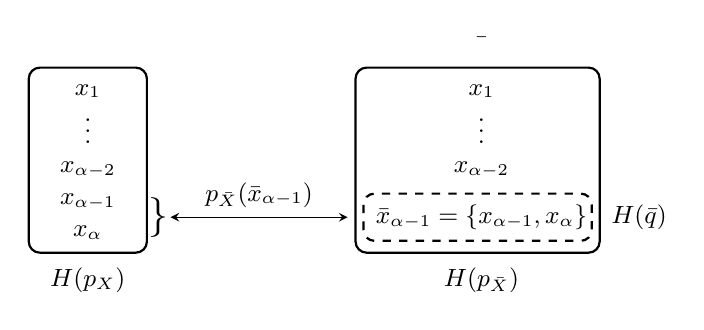
\begin{tikzpicture}
\shorthandoff{>}
%
% Ensemble \X
\draw(0,3) node{\small $\X$};
\draw(0,2.4) node{\small $x_1$};
\draw(0,2) node{\small $\vdots$};
\draw(0,1.4) node{\small $x_{\alpha-2}$};
\draw(0,1) node{\small $x_{\alpha-1}$};
\draw(0,.6) node{\small $x_{\alpha}$};
\draw(0,0) node{\small $H(p_X)$};
\draw[thick,rounded corners] (-.75,.35) rectangle (.75,2.7);
%
% Ensemble \bar{\X}
%
\draw(5,3) node{\small $\bar{\X}$};
\draw(5,2.4) node{\small $x_1$};
\draw(5,2) node{\small $\vdots$};
\draw(5,1.4) node{\small $x_{\alpha-2}$};
\draw(5,.8) node{\small $\bar{x}_{\alpha-1} = \{ x_{\alpha-1} , x_\alpha\}$};
\draw(5,0) node{\small $H(p_{\bar{X}})$};
\draw(7,.8) node{\small $H(\bar{q})$};
\draw[dashed,thick,rounded corners] (3.5,.5) rectangle (6.4,1.1);
\draw[thick,rounded corners] (3.4,.35) rectangle (6.5,2.7);
%
% juntando 2 estados VER PROBLEMA CON LA FLECHA
\draw(.9,.8) node{\Large $\}$};
\draw[>=stealth,<->] (1.05,.8)--(3.3,.8);
\draw (2.175,.8) node[above]{\small $p_{\bar{X}}(\bar{x}_{\alpha-1})$};
\end{tikzpicture} \end{center}
  %
  \leyenda{Ilustraci\'on de  la propiedad  de recursividad, que  cuantifica como
    decrece  la  entrop\'ia  en  un  conjunto  cuando  se  juntan  dos  estados,
    relacionando   la  entrop\'ia   total,  la   entrop\'ia  despu\'es   del  la
    agrupaci\'on y la entrop\'ia interna a los dos estados juntados.}
  %
  \label{Fig:SZ:Recursividad}
  \end{figure}
  %
%
\setcounter{PropConcavidad}{\value{enumi}}
\item\label{Prop:SZ:concavidad}  {\it Concavidad:}  la  entrop\'ia es  c\'oncava
  ($-H$         es         convexa,        ver         Def.~\ref{Def:MP:convexa}
  pagina~\pageref{Def:MP:convexa}), en  el sentido de  que la entrop\'ia  de una
  combinaci\'on convexa de distribuciones  (mezcla) de probabilidades es siempre
  mayor o igual a la combinaci\'on convexa de entrop\'ias:
  %
  \[
  \forall \:  \{ \pi_i \}_{i=1}^n, \quad  0 \le \pi_i \le  1, \quad \sum_{i=1}^n
  \pi_i  = 1  \quad \mbox{and  cualquier  conjunto de  distribuciones} \quad  \{
  p_{(i)} \}_{i=1}^n,
  \]
  %
  \[
  H\left( \sum_{i=1}^n \pi_i \, p_{(i)} \right) \ge \sum_{i=1}^n \pi_i H(p_{(i)}).
  \]
  %
  Esta relaci\'on es conocida tambi\'en como desigualdad de Jensen~\cite{Jen06}.
  Es una consecuencia directa de la  convexidad de la funci\'on $\phi: t \mapsto
  t \log  t$, como ilustrado en la  figura Fig.~\ref{Fig:SZ:Concavidad}-(a).  La
  figura  Fig.~\ref{Fig:SZ:Concavidad}-(b)  ilustra como  se  puede obtener  una
  mezcla  de distribuciones  de dos  probabilidad $p_{(1)}$  (dado  izquierda) y
  $p_{(2)}$ (dado  derecho) haciendo  una elecci\'on aleatoria  a partir  de una
  moneda en  este ejemplo (probabilidad  $\pi_1 = 1  - \pi_2$ de elegir  el dado
  izquierda).\newline
  %
  \begin{figure}[h!]
  %
  \begin{center} \begin{tikzpicture}
\shorthandoff{>}
%
% Concavidad de - u log u
\begin{scope}[xscale=3,yscale=2.5]
\pgfmathsetmacro{\u}{.2};
\pgfmathsetmacro{\v}{1.25};
\pgfmathsetmacro{\l}{.7};
%
\draw[>=stealth,->] (-.5,0)--(1.6,0) node[right]{\small $t$};
\draw[>=stealth,->] (0,-.7)--(0,{1.5*log2(1.5)}) node[above]{\small $\phi(t) = t \log t$};
\draw[thick,domain=.005:1.5,samples=200] (0,0)-- plot (\x,{\x*log2(\x)});
\draw[dashed] (\u,{\u*log2(\u)})--(\v,{\v*log2(\v)});
\draw (\u,0)--(\u,-.05) node[below]{\small $t_1$};
\draw (\v,0)--(\v,-.05) node[below]{\small $t_2$};
%
\draw[dashed] ({\l*\u+(1-\l)*\v},.05) node[above]{\small $\pi_1 t_1 + \pi_2 t_2$}
--({\l*\u+(1-\l)*\v},{(\l*\u+(1-\l)*\v)*log2(\l*\u+(1-\l)*\v)});
%
% l phi(u) + (1-l) phi(v)
\draw[dotted]
({\l*\u+(1-\l)*\v},{\l*\u*log2(\u)+(1-\l)*\v*log2(\v)})--(-.05,{\l*\u*log2(\u)+(1-\l)*\v*log2(\v)})
node[left]{\small $\pi_1 \phi(t_1) + \pi_2 \phi(t_2)$};
%
% phi(l u + (1-l) v)
\draw[dotted]
({\l*\u+(1-\l)*\v},{(\l*\u+(1-\l)*\v)*log2(\l*\u+(1-\l)*\v)})--
(-.05,{(\l*\u+(1-\l)*\v)*log2(\l*\u+(1-\l)*\v)})
node[left]{\small $\phi(\pi_1 t_1 + \pi_2 t_2)$};
\end{scope}
%
%
% Concavidad / mezcla
\begin{scope}[xshift=8.5cm]
\draw(0,1.25) node{\includegraphics[width=3cm]{TIKZ_SZ/DosDados}};
\draw(-.5,2.5) node{\small $p_1$};
\draw(1,2) node{\small $p_2$};
\draw(2.7,1) node{\small $\pi_1 p_1 + \pi_2 p_2$};
\draw(-.25,-1) node{
\includegraphics[width=1cm]{TIKZ_SZ/Moneda}};
\draw[>=stealth,->,thick] (-.3,-.35)--(-.75,.45);
\draw (-.525,0) node[left]{\small $\pi_1$};
\draw[>=stealth,->,thick] (-.2,-.35)--(.3,.45);
\draw (.05,0) node[right]{\small $\pi_2 = 1-\pi_1$};
\end{scope}
%
\draw (1.25,-2.25) node{(a)};
\draw (8.25,-2.25) node{(b)};
\end{tikzpicture} \end{center}
  %
  \leyenda{(a) $\phi(t)  = t \log t$ es  convexa: la curva es  siempre debajo de
    sus cuerdas; entonces, cada promedio de $\phi(t_1)$ y $\phi(t_2)$ estando en
    la cuerda juntando  estos puntos, queda arriba de la  funci\'on tomada en el
    promedio de $t_1$ y $t_2$.  Escribiendo eso para (m\'as de dos puntos) sobre
    los $\sum_i \pi_i \, p_{(i)}(x)$ y sumando sobre los $x$  da la desigualdad de
    Jensen.  (b) Ilustraci\'on de  una distribuci\'on de mezcla, ac\'a mezclando
    $p_{(1)}$ y $p_{(2)}$  a partir de una tercera  variable aleatoria (ac\'a de
    Bernoulli).}
  %
  \label{Fig:SZ:Concavidad}
  \end{figure}
%
\setcounter{PropSchurConcavidad}{\value{enumi}}
\item\label{Prop:SZ:Schurconcavidad}  {\it Schur-concavidad:}  como se  lo puede
  querrer, lo  m\'as ``concentrado'' es  una distribuci\'on de  probabilidad, lo
  menos   hay  incerteza,   y  entonces   lo   m\'as  peque\~no   debe  ser   la
  entrop\'ia.  Esta propiedad intuitiva  se resuma  a partir  de la  noci\'on de
  mayorizaci\'on.
  %
  \begin{definicion}[Mayorizaci\'on]\label{Def:SZ:Mayorizacion}
    Un vector de  probabilidad (distribuci\'on) $p$ mayorizado por  un vector de
    probabilidad (distribuci\'on) $q$, notado $p \prec q$, se define como:
    %
    \[
    p  \prec   q  \qquad  \mbox{ssi}  \qquad   \sum_{i=1}^k  p_i^\downarrow  \le
    \sum_{i=1}^k q_i^\downarrow, \quad  1 \le k < \alpha  \qquad \mbox{y} \qquad
    \sum_{i=1}^\alpha p_i^\downarrow = \sum_{i=1}^\alpha q_i^\downarrow
    \]
    %
    (las \'ultimas sumas siendo igual a 1).  Si los alfabetos de definici\'on de
    \ $p$ \ y  \ $q$ \ son de tama\~nos diferentes, \  $\alpha$ \ es el tama\~no
    lo m\'as  grande y  la distribuci\'on  sobre el alfabeto  lo m\'as  corto es
    completada por  estados de probabilidad 0  (recordar que no va  a cambiar la
    entrop\'ia).
  \end{definicion}
  %
  La  Schur-concavidad  se  traduce  por  la  relaci\'on
  %
  \[
  p \prec  q \quad \Rightarrow  \quad H(p) \ge  H(q).
  \]
  %
  Fijense de  que las cotas  sobre $H$ pueden  ser vistas como  consecuencias de
  esta desigualdad: la  distribuci\'on cierta mayoriza cualquiera distribuci\'on
  y  cualquiera distribuci\'on  mayoriza la  distribuci\'on uniforme~\cite[p.~9,
  (6)-(8)]{MarOlk11}.  Adem\'as, de la Schur-concavidad se obtiene que
  %
  \[
  H\left( \begin{bmatrix}  \frac1\alpha & \cdots  & \frac1\alpha \end{bmatrix}^t
  \right) \quad \mbox{es una funci\'on creciente de } \alpha.
  \]
  %
  La prueba  de la  Schur-concavidad se  apoya sobre la  desigualdad de  Schur o
  Hardy-Littlewood-P\'olya    o     Karamata~\cite{Sch23,    HarLit29,    Kar32,
    HarLit52},~\cite[Cap.~3,                                 Prop.~C.1]{MarOlk11}
  o~\cite[Teorema~II.3.1]{Bha97}: $t \prec t' \: \Rightarrow \: \sum_i \phi(t_i)
  \le  \sum_i  \phi(t'_i)$  para  cualquiera  funci\'on  $\phi$  convexa.  Basta
  considerar $\phi(t) = t \log t$ para concluir.
\end{propiedades}
%
% Ver Schur-Ostrowski f  sym, Scur-convexe ssi (xi - xj)  (df/dx_i - df/dxj) \ge
% 0, 1 \le i \ne j \le alpha


En muchos  casos, uno tiene que  trabajar con varias  variables aleatorias. Para
simplificar las notaciones, consideramos  un par de variables \ $X$ \  y \ $Y$ \
definidas respectivamente sobre los alfabetos \ $\X$  \ y \ $\Y$ \ de cardinal \
$\alpha = |\X|$ \ y \ $\beta = |\Y|$.  Tal par de variables puede ser vista como
una  variable $(X,Y)$  definida sobre  el alfabeto  $\X \times  \Y$  de cardinal
$\alpha \beta$ tal que se  define naturalmente la entrop\'ia para esta variable;
tal entrop\'ia es llamada {\it entrop\'ia conjunta} de $X$ y $Y$:
%
\begin{definicion}[Entrop\'ia conjunta]\label{Def:SZ:EntropiaConjunta}
  Sean \ $X$ \ e \ $Y$  \ dos variables aleatorias definidas sobre los alfabetos
  discretos \  $\X$ \ y \ $\Y$,  de cardinal \ $\alpha  = |\X| < +\infty$  \ y \
  $\beta  =  |\Y|   <  +\infty$  \  respectivamente.   Sea   \  $p_{X,Y}$  \  la
  distribuci\'on de probabilidad conjunta de \ $X$ \ e \ $Y$, \ \ie $ \forall \,
  (x,y) \in \X \times  \Y, \quad p_{X,Y}(x,y) = P( (X = x) \cap  (Y = y) )$.  La
  entrop\'ia conjunta de Shannon de las variables  \ $X$ \ e \ $Y$ \ es definida
  por
  %
  \[
  H(p_{X,Y}) =  H(X,Y) = -  \sum_{(x,y) \in \X  \times \Y} p_{X,Y}(x,y)  \, \log
  p_{X,Y}(x,y),
  \]
  %
  con la convenci\'on \ $0 \log 0 = 0$.
\end{definicion}

A partir de esta definici\'on,  aparecen otras propiedades importantes, sino que
fundamentales, de la entrop\'ia de Shannon.
%
\begin{propiedades}
\item\label{Prop:SZ:aditividad} {\it Aditividad:}  la entrop\'ia conjunta de dos
  variables aleatorias  \ $X$  \ e \  $Y$ \underline{independientes} se  suma, y
  rec\'iprocamente:
  %
  \[
  X \: \mbox{e} \: Y \: \mbox{independientes} \quad \Leftrightarrow \quad H(X,Y)
  =  H(X) +  H(Y).
  \]
  %
  Dicho de otra manera, para dos variables aleatorias, la incerteza global es la
  suma   de  las  incertezas   de  cada   variable  individual.    La  propiedad
  ``$\Rightarrow$'' es consecuencia directa de \ $p_{X,Y}(x,y) = p_X(x) p_Y(y)$.
  Se va  a probar en  la secci\'on siguiente  la rec\'iproca. Esta  propiedad se
  escribe tambi\'en
  %
  \[
  H\left( p_X \otimes p_Y \right) = H\left( p_X \right) + H\left( p_Y \right),
  \]
  %
  donde  $\otimes$ es el  producto de  Kronecker~\footnote{Recuerdense de  que \
    $p_X  \otimes p_Y$ es  un vector  de tama\~no  $\alpha \beta$  de componente
    $(i-1)  \alpha +  j$-\'esima \  $p_X(x_i)  \, p_Y(y_j),  \quad 1  \le i  \le
    \alpha, \: 1 \le  j \le \beta$.  Se lo puedo ver  tambi\'en como un producto
    tensorial  o externo  de \  $p_X$ \  definido sobre  \ $\X$  \ y  \  $p_Y$ \
    definido sobre \  $\Y$, \ el producto tensorial siendo  definido sobre \ $\X
    \times      Y$.       Ver      nota      de      pie~\ref{foot:MP:Kronecker}
    pagina~\pageref{foot:MP:Kronecker}.}.   Se  generaliza  sencillamente  a  un
  conjunto de variables aleatorias $\{ X_i \}_{i=1}^n$ (o, equivalentemente a un
  producto de Kronecker de un conjunto de vectores de probabilidades).
%
\item\label{Prop:SZ:subaditividad} {\it  Sub-aditividad:} la entrop\'ia conjunta
  de dos variables  aleatorias $\{ X_i \}_{i=1}^n$ es siempre  menor que la suma
  de cada entrop\'ia individual:
  %
  \[
  H(X_1,\ldots,X_n)  \,  \le \,  \sum_{i=1}^n  H(X_i)  \qquad \mbox{\ie}  \qquad
  H\left(  p_{X_1,, \ldots  , X_n}  \right) \,  \le \,  H\left(  p_{X_1} \otimes
    \cdots \otimes p_{X_n} \right) = \sum_{i=1}^n H\left( p_{X_i} \right).
  \]
  %
  Dicho de otra manera, las variables aleatorias pueden compartir informaci\'on,
  de  tal  manera que  la  entrop\'ia  global sea  menor  que  la  suma de  cada
  entrop\'ia.  De la  propiedad anterior, se obtiene la  igualdad si y solamente
  si los $X_i$ son independientes.
%
\item\label{Prop:SZ:superaditividad}   {\it  Super-aditividad:}   la  entrop\'ia
  conjunta de dos variables aleatorias  $\{ X_i \}_{i=1}^n$ es siempre mayor que
  cualesquiera de las entrop\'ias individuales
  %
  \[
  H(X_1,\ldots,X_n) \, \ge \, \max_{1 \le i \le n} H(X_i).
  \]
\end{propiedades}

Es  importante notar  que existen  varios enfoques  basados sobre  una  serie de
axiomas, dando lugar a la definici\'on de la entrop\'ia tal como definida. Estos
axiomas   son   conocidos   como   axiomas   de  Shannon-Khinchin   y   son   la
continuidad~\ref{Prop:SZ:continuidad},  la maximalidad~\ref{Prop:SZ:cotamaxima},
la           expansabilidad~\ref{Prop:SZ:expansabilidad}           y          la
aditividad~\ref{Prop:SZ:aditividad}.  Existen varios otros conjuntos de axiomas,
conduciendo  tambi\'en a  la entrop\'ia  de Shannon  (ver~\cite[Sec.~6]{Sha48} o
\cite{ShaWea64, Fad56, Fad58, Khi57, Ren61}, entre otros).

Para  una  serie de  variables  aleatorias,  $X_1,  X_2, \ldots$,  representando
s\'imbolos, se  puede definir una  entrop\'ia por s\'imbolo como  una entrop\'ia
conjunta  divido por el  n\'umero de  s\'imbolos, $\frac{H(X_1,\ldots,x_n)}{n}$,
as\'i que una tasa de entrop\'ia cuando $n$ va al infinito.
%
\begin{definicion}[Tasa de entrop\'ia]\label{Def:SZ:TasaDeEntropia}
  Sea $X \equiv \{ X_i \}_{i  \in \Nset^*}$ una serie de variables aleatorias, o
  proceso estoc\'astico.  La tasa de entrop\'ia del proceso es definida por
  %
  \[
  \H(X) = \lim_{n \to \infty} \frac{H(X_1,\ldots,X_n)}{n}.
  \]
  %
\end{definicion}
%
\noindent Esta  cantidad siempre existe  porque $\displaystyle H(X_1 ,  \ldots ,
X_n) \le \sum_{i=1}^n H(X_i) \le \sum_{i=1}^n  \log \alpha_i \le n \max_{1 \le i
  \le n} \alpha_i$  donde los $\alpha_i$ son los cardinales  de los alfabetos de
definici\'on de los $X_i$.

\

Se termina esta subsecci\'on con el caso de variables discretas definidas sobre
un  alfabeto $\X$ de  cardinal infinito  $|\X| =  + \infty$,  por ejemplo  $\X =
\Nset$.   Por analog\'ia,  se puede  siempre definir  la entrop\'ia  como  en la
definici\'on Def.~\ref{Def:SZ:Shannon}. Esta extensi\'on resuelta delicada dando
de que unas propiedades se perdien.  Por ejemplo, la entrop\'ia no queda acotada
por arriba  como se  lo puede  probar para la  distribuci\'on de  probabilidad \
$\displaystyle p(x)  \propto \frac{1}{(x+2) \left(  \log (x+2) \right)^2},  \: x
\in \Nset$, correctamente  normalizada ($\propto$ significa ``proporcional a''):
\ $\displaystyle \frac{\log \log(x+2)}{(x+2) \left( \log (x+2) \right)^2} \ge 0$
\  y  \ la  serie  \  $\displaystyle \sum_x  \frac{1}{(x+2)  \log  (x+2)}$ \  es
divergente,  as\'i que  la serie  \ $\displaystyle  - \sum_x  p(x) \log  p(x)$ \
diverge.

% ================================= Entropia diferencial

\subseccion{Entrop\'ia diferencial}
\label{Ssec:SZ:Diferencial}

Volviendo  a  la  definici\'on  Def.~\ref{Def:SZ:Shannon} de  la  entrop\'ia  de
Shannon,  usando   el  operador   $\Esp$  promedio  estad\'istico   o  esperanza
matem\'atica,  se  puede  reescribir  la  entrop\'ia de  Shannon  como  $H(X)  =
\Esp\left[ - \log p_X(X) \right]$.  Con este punto de vista, es f\'acil extender
la definici\'on de la  entrop\'ia para variables aleatorias continuas admitiendo
una densidad de  probabilidad.  Eso da lugar  a lo que es conocido  como la {\it
  entrop\'ia diferencial}:

\begin{definicion}[Entrop\'ia diferencial]\label{Def:SZ:EntropiaDiferencial}
  Sea  $X$   una  variable  aleatoria   continua  admitiendo  una   densidad  de
  probabilidad \ $p_X$, definida sobre \ $\Rset^d$  \ y \ $X(\Omega) = \X = \{ x
  \in  \Rset^d:  \:  p_X(x)  >  0  \}  \subseteq \Rset^d$  \  el  soporte  de  \
  $p_X(x)$. La entrop\'ia diferencial de la variable $X$ es definida por
  %
  \[
  H(p_X) = H(X) = - \int_\X p_X(x) \, \log p_X(x) \, dx
  \]
  %
  (con la  convenci\'on $0 \log  0 = 0$,  se puede escribir la  integraci\'on en
  $\Rset^d$).
\end{definicion}
%
Como en el caso discreto, para $X = (X_1,\ldots,X_d)$, esta entrop\'ia de $X$ es
dicha entrop\'ia conjunta de los componentes $X_i$.

Como se lo va a ver, la entrop\'ia diferencial no tiene la misma significaci\'on
de  incerteza,  siendo de  que  depende no  solamente  de  la distribuci\'on  de
probabilidad, sino que  de los estados tambi\'en.  M\'as all\'a,  no se la puede
ver como l\'imite  continua de un caso discreto: a trav\'es  de tal l\'imite, se
va  a ver  que se  llama diferencial,  a causa  del efecto  de  la ``diferencial
$dx$''.  Para ilustrar este hecho, consideramos una variable aleatoria escalar \
$X$ \ y \ $p_X$ \ su densidad de probabilidad de soporte $\Rset$.  Sea \ $\Delta
> 0$  \ y sea el alfabeto  $\X^\Delta = \{ x_k  \}_{k \in \Zset}$ \  donde los \
$x_k$ se definen tal que $\displaystyle p_X(x_k) \Delta = \int_{k \Delta}^{(k+1)
  \Delta}     p_X(x)    \,     dx$,    como     ilustrado    en     la    figura
Fig.~\ref{Fig:SZ:CuantificacionX}.  Se  define la variable  aleatoria discreta \
$X^\Delta =  \sum_k x_k  \un_{(X \in  [k \Delta ,  (k+1) \Delta  ))}$ \  sobre \
$\X^\Delta$  \ tal  que  \ $P(X^\Delta  =  x_k) =  p_{X^\Delta}(x_k) =  p_X(x_k)
\Delta$.  \ Se puede ver \ $X^\Delta$ \ como la versi\'on cuantificada de \ $X$,
\ con \  $X^\Delta = x_k$ \ cuando \  $X \in [k \Delta , (k+1)  \Delta )$.  \ Al
rev\'es,  a\'un  que  sea  delicado,  se  puede interpretar  \  $X$  \  como  el
``l\'imite'' de \ $X^\Delta$  \ cuando \ $\Delta$ \ tiende a  0. Ahora, es claro
de que
%
\begin{eqnarray*}
H(X^\Delta) & = & - \sum_k p_{X^\Delta}(x_k) \log p_{X^\Delta}(x_k)\\[2.5mm]
%
& = & - \log \Delta - \sum_k \Big( p_X(x_k) \log p_X(x_k) \Big) \, \Delta
\end{eqnarray*}
%
lo que se escribe tambi\'en
%
\[
H(X^\Delta)  + \log  \Delta =  - \sum_k  \Big( p_X(x_k)  \log p_X(x_k)  \Big) \,
\Delta.
\]
%
Entonces, de la integraci\'on de Riemann sale que
%
\[
\lim_{\Delta \to 0} \left( H(X^\Delta) + \log \Delta \right) = H(X).
\]
%
Dicho de otra manera,  la entrop\'ia diferencial de $X$ no es  el l\'imite de la
entrop\'ia de su versi\'on cuantificada:  aparece con la entrop\'ia el t\'ermino
``diferencial'' $\log \Delta$.
%
\begin{figure}[h!]
%
\begin{center} 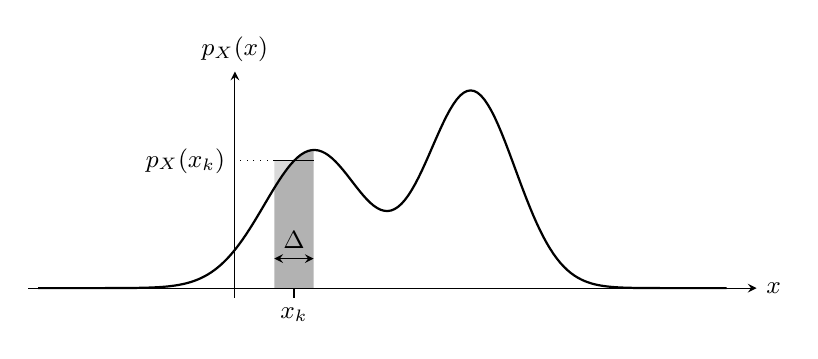
\begin{tikzpicture}
\shorthandoff{>}
%
% Cuantificacion de X
\begin{scope}[xscale=2.5,yscale=2.5]
%
\pgfmathsetmacro{\c}{.4};
\pgfmathsetmacro{\d}{1.2};
\pgfmathsetmacro{\s}{8};
\pgfmathsetmacro{\t}{10};
\pgfmathsetmacro{\a}{.7};
\pgfmathsetmacro{\b}{1};
%
\pgfmathsetmacro{\xk}{.3};
\pgfmathsetmacro{\dx}{.2};
%
% funcion para dibujar una distribucion bimodal (ilustracion de la cuantificacion)
\pgfmathdeclarefunction{bimod}{1}{\pgfmathparse{(\a*exp(-\s*(#1-\c)^2)+\b*exp(-\t*(#1-\d)^2))}}
%
\draw[>=stealth,->] (-1.05,0)--(2.65,0) node[right]{\small $x$};
\draw[>=stealth,->] (0,-.05)--(0,1.1) node[above]{\small $p_X(x)$};
%
% lei de proba
\draw[thick,domain=-1:2.5,samples=200] plot (\x,{bimod(\x)});
%
% dominio alrededor de xk
\fill[domain=\xk-\dx/2:\xk+\dx/2,samples=20,opacity=.3]
({\xk-\dx/2},0)-- plot (\x,{bimod(\x)})--({\xk+\dx/2},0);
%
% xk y Delta
\draw (\xk,0)--(\xk,-.05) node[below]{\small $x_k$};
\draw[>=stealth,<->] ({\xk-\dx/2},.15)--({\xk+\dx/2},.15);
\draw (\xk,.15) node[above]{\small $\Delta$};
%
% recta sobre Delta a altura de p(xk)
\draw ({\xk+\dx/2},{bimod(\xk)})-- ({\xk-\dx/2},{bimod(\xk)});
\draw[dotted] ({\xk-\dx/2},{bimod(\xk)})--(0,{bimod(\xk)})
 node[left]{\small $p_X(x_k)$};
%
% dominio equivalente alrededo de xk
\fill[domain=\xk-\dx/2:\xk,samples=20,opacity=.15]
plot (\x,{bimod(\x)})--({\xk-\dx/2},{bimod(\xk)});
\end{scope}
\end{tikzpicture} \end{center}
%
\leyenda{Densidad  de probabilidad  $p_X$  de $X$,  construcci\'on del  alfabeto
  $\X^\Delta$ donde se define la versi\'on cuantificada $X^\Delta$ de $X$ con su
  distribuci\'on discreta de probabilidad  $p_{X^\Delta}$. La superficie en gris
  oscuro es igual a la superficie definida por el rect\'angulo en gris claro.}
%
\label{Fig:SZ:CuantificacionX}
\end{figure}
%

M\'as  all\'a de esta  notable diferencia  entre la  entrop\'ia y  la entrop\'ia
diferencial, la \'ultima depende de los estados,  es decir que si $Y = g(X)$ con
$g$  biyectiva,  no se  conserva  la  entrop\'ia,  \ie \underline{se  pierde  la
  propiedad~\ref{Prop:SZ:biyeccion}} del caso discreto:
%
\begin{eqnarray*}
H(Y) & = & - \int_{\Rset^d} p_Y(y) \log p_Y(y) \, dy\\[2.5mm]
%
& = &  - \int_{\Rset^d} p_Y(g(x)) \log p_Y(g(x)) \, |\Jac_g(x)| \, dx\\[2.5mm]
%
& = & - \int_{\Rset^d} p_Y(g(x)) \Big( \log \big( p_Y(g(x)) \, |\Jac_g(x)| \big) -
\log |\nabla^t g(x)| \Big) \, |\Jac_g(x)| \, dx
\end{eqnarray*}
%
donde $\Jac_g$ es la matriz Jacobiana
% la  matriz de componentes $\frac{\partial g_i}{\partial x_j}$,
%Jacobiano  
de  la  transformaci\'on  \   $g:  \Rset^d  \mapsto  \Rset^d$  \  
%($g
%\equiv [ g_1(x_1 , \ldots  , x_d) \quad  \cdots \quad g_d(x_1 ,  \ldots ,
%  x_d) ]^t$)
\ y  \ $|\cdot|$  representa el  valor absoluto del  determinante de  la matriz.
Recordando      que     $p_X(x)      =      p_Y(g(x))     |\Jac_g(x)|$      (ver
subsecci\'on~\ref{Ssec:MP:Transformacion},
pagina~\pageref{Ssec:MP:Transformacion}), se obtiene la propiedad siguiente:
%
\begin{propiedadesC}\setcounter{enumi}{\value{PropBiyeccion}}
%
\item\label{Prop:SZ:biyeccionC}
Para  cualquiera biyecci\'on $g:  \Rset^d \mapsto  \Rset^d$
  %
  \[
  H(g(X)) = H(X) + \int_{\Rset^d} p_X(x) \log |\Jac_g(x)| \, dx,
  \]
  %
  donde el \'ultimo t\'ermino, $\Esp\left[  \log |\Jac_g(X)| \right]$ no vale cero
  en general.  En particular, si $H$ es invariante bajo una translaci\'on,
  %
  \[
  H(X+b) = H(X) \quad \forall \: b \in \Rset^d,
  \]
  %
  no  es invariante  por cambio  de escala,
  %
  \[
  H(a X) = H(X) + \log |a| \quad \forall \: a \in \Rset^*.
  \]
\end{propiedadesC}
%
Esta \'ultima  relaci\'on queda v\'alido  para $a$ matriz invertible.   Por esta
\'ultima  relaci\'on, se puede  ver que,  dado $X$,  cuando $a$  tiende a  0, la
entrop\'ia de $a X$ tiende a  $-\infty$.  Es decir que, para $a$ suficientemente
peque\~no,  se  puede  tener $H(a  X)  <  0$,  as\'i que  \underline{se  pierde}
tambi\'en   \underline{la   positividad~\ref{Prop:SZ:positividad}}.   Por   esta
perdida, se quita definitivamente la interpretaci\'on de incerteza/informaci\'on
que hubiera podido tener la entrop\'ia diferencial.

A veces, se usa lo que es llamado potencia entr\'opica:
%
\begin{definicion}[Potencia entr\'opica]
  Sea $X$ una variable aleatoria $d$-dimensional. La potencia entr\'opica de $X$
  es definida por
  %
  \[
  N(X) = \frac{1}{2 \pi \e} \exp\left( \frac2d H(X) \right).
  \]
\end{definicion}
%
\noindent Por construcci\'on, $N(X) \ge 0$.  Adem\'as, en el caso continuo, $N(a
X+b)  =  |a|^2 N(X)$  (queda  v\'alido para  una  matriz  $a$ invertible):  esta
propiedad puede justificar  la idea de ``potencia''; adem\'as  $N(a X+b)$ tiende
naturalmente a  cero cuando $a$  tiende a cero.   Se recupera as\'i  la noci\'on
informacional a trav\'es  de $N$ en este  contexto ($a X + b$  ``tiende'' a $b$,
variable determinista).

Si se pierde la propiedad de invarianza bajo una biyecci\'on, sorprendentemente,
se conserva la entrop\'ia bajo el equivalente continuo del rearreglo.
%
\begin{definicion}[Rearreglo sim\'etrico]\label{Def:SZ:rearreglo}
  Sea $\P \subset \Rset^d$ abierto de  volumen finito $|\P| < +\infty$.  El {\it
    rearreglo sim\'etrico} $\P^\downarrow$  de $\P$ es la bola  centrada en 0 de
  mismo volumen que $\P$, \ie
  %
  \[
  \P^\downarrow  = \left\{  x  \in  \Rset^d \,  :  \: \frac{2  \pi^{\frac{d}{2}}
      |x|^d}{\Gamma\left(\frac{d}{2}\right)} \le |\P| \right\},
  \]
  %
  donde  $|\cdot|$  denota  la   norma  euclideana.   Eso  es  ilustrado  figura
  Fig.~\ref{Fig:SZ:ensemblerearreglado}-a.\newline  Sea  $p_X$  una densidad  de
  probabilidad y sea $\P_t = \{ y \, : \: p_X(y) > t \}$ para cualquier $t > 0$,
  sus conjuntos  de niveles.  La densidad de  probabilidad~\footnote{Se proba de
    que  esta funci\'on,  positiva por  definici\'on, suma  a 1.   Adem\'as, por
    construcci\'on,  depende  \'unicamente  de   $|x|$  y  decrece  con  $|x|$.}
  rearreglada sim\'etrico $p^\downarrow_X$ de $p_X$ es definida por
  %
  \[
  p^\downarrow_X(x)  =  \int_0^{+\infty}  \un_{\P_u^\downarrow}(x) \,  du.
  \]
  %
  (recuerdense de que $\un_A$ es el indicator  del conjunto $A$)
  % , \ie $\un_A(x) = 1$ si $x \in A$ y cero sino.
\end{definicion}
%
Del hecho  de que $\forall \, t  < \tau \: \Leftrightarrow  \: \P_\tau \subseteq
\P_t  \:  \Leftrightarrow \:  \P_\tau^\downarrow  \subseteq \P_t^\downarrow$  es
sencillo   ver   que   si   $x   \in  \P_\tau^\downarrow$,   entonces   $x   \in
\P_t^\downarrow$,  lo que  conduce a  $p_X^\downarrow(x) >  \tau$  y vice-versa.
M\'as  all\'a, sobre  $\P_{\tau+d\tau}  \backslash \P_\tau$  la funci\'on  $p_X$
``vale''   $\tau$   \   y   \   sobre   $\P_{\tau+d\tau}^\downarrow   \backslash
\P_\tau^\downarrow$  la funci\'on $p_X^\downarrow$  ``vale'' tambien  $\tau$, lo
que  da \  $\displaystyle  \int_{\P_\tau^\downarrow} p_X^\downarrow(x)  \, dx  =
\int_{\P_\tau} p_X(x)  \, dx$ \  (ver~\cite{LieLos01, WanMad04} para  une prueba
m\'as  rigurosa).   La representaci\'on  de  la  definici\'on  es conocida  como
representaci\'on  en  capas  de  pastel  (``layer cake''  en  ingles).   Eso  es
ilustrado en la figura Fig.~\ref{Fig:SZ:ensemblerearreglado}-b
  %
  \begin{figure}[h!]
  %
  \begin{center} 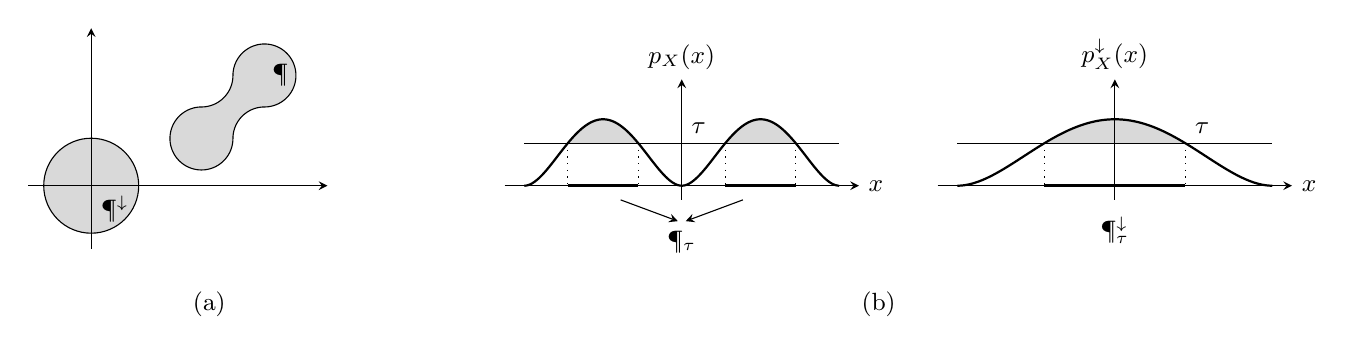
\begin{tikzpicture}
\shorthandoff{>}
%
\begin{scope}[scale=.4]
% Superficia 2*3 pi/4  + 2*2 - 2*pi/4 = 4+pi
\filldraw[draw=black,fill=gray!30]
   plot [domain=0:-270,samples=200] ({cos(\x)+3.5},{sin(\x)+1.5})
-- plot [domain=-90:0,samples=200] ({cos(\x)+3.5},{sin(\x)+3.5})
-- plot [domain=180:-90,samples=200] ({cos(\x)+5.5},{sin(\x)+3.5})
-- plot [domain=90:180,samples=200] ({cos(\x)+5.5},{sin(\x)+1.5})
-- cycle;
\draw (6,3.5) node {\small $\P$};
%
% superficia rearreglada
\filldraw[draw=black,fill=gray!30] (0,0) circle ({sqrt(1+4/pi)});
\draw (.75,-.75) node {\small $\P^\downarrow$};
%
% ejes
\draw[>=stealth,->] (-2,0)--(7.5,0);
\draw[>=stealth,->] (0,-2)--(0,5);
%
\end{scope}
%
%
%----------------------------------------
%
% p_X(x), P_tau...
\begin{scope}[xshift=7.5cm,yscale=1.8]
\pgfmathsetmacro{\t}{.3};
\pgfmathsetmacro{\xt}{sqrt(1-sqrt(32*\t/15))};
\pgfmathsetmacro{\dx}{5.5};% shift para p*(x)
\pgfmathdeclarefunction{studr}{1}{\pgfmathparse{(15/32)*((1-(#1)^2)^2)}}; %Student-r
%
% mezcla de Student-r 15/16 * (1-x^2)^2 (nu = 5) centrados en -1 y 1
% 15/32 (1-(x-a)^2)^2 > t iif (x-a)^2 < 1-sqrt(32*t/15)
% i.e. a-sqrt(1-sqrt(32*t/15)) < x < a+sqrt(1-sqrt(32*t/15))
\fill[domain=-1-\xt:-1+\xt,fill=gray!30] plot(\x,{studr(\x+1)}); % p(x) > tau, x < 0
\fill[domain=1-\xt:1+\xt,fill=gray!30] plot(\x,{studr(\x-1)}); % p(x) > tau, x > 0
\draw[thick,domain=-2:0,samples=100] plot(\x,{studr(\x+1)}); % p(x), x < 0
\draw[thick,domain=0:2,samples=100] plot(\x,{studr(\x-1)}); % p(x), x > 0
\draw (-2,\t)--(2,\t); \draw (0,\t) node[above right]{\small $\tau$}; % y = tau
%
% dominio P_tau
\draw[dotted] ({-1-\xt},{studr(\xt)})--({-1-\xt},0);
\draw[dotted] ({-1+\xt},{studr(\xt)})--({-1+\xt},0);
\draw[very thick] ({-1-\xt},0)--({-1+\xt},0);
\draw[>=stealth,->] ({-1+\xt/2},-.1)--(-.05,-.25);
%
\draw[dotted] ({1-\xt},{studr(\xt)})--({1-\xt},0);
\draw[dotted] ({1+\xt},{studr(\xt)})--({1+\xt},0);
\draw[very thick] ({1-\xt},0)--({1+\xt},0);
\draw[>=stealth,->] ({1-\xt/2},-.1)--(.05,-.25);
%
\draw (0,-.25) node[below]{\small $\P_\tau$};
%
% ejes
\draw[>=stealth,->] (-2.25,0)--(2.25,0) node[right]{\small $x$};
\draw[>=stealth,->] (0,-.1)--(0,.75) node[above]{\small $p_X(x)$};
%
%---------------------------
%
% 15/32 (1-(x-a)^2)^2 > t iif (x-a)^2 < 1-sqrt(32*t/15)
% i.e. a-sqrt(1-sqrt(32*t/15)) < x < a+sqrt(1-sqrt(32*t/15))
% Volumen 2*sqrt(1-sqrt(32*t/15))
% Por simetria, P_t* = [-2*sqrt(1-sqrt(32*t/15)) , 2*sqrt(1-sqrt(32*t/15))]
% da f*(x) = 15/32 (1-x^2/4)^2
\fill[domain=-2*\xt:2*\xt,fill=gray!30] plot({\x+\dx},{studr(.5*\x)}); % p*(x) > tau
\draw[thick,domain=-2:2,samples=200] plot({\x+\dx},{studr(.5*\x)});
\draw ({-2+\dx},\t)--({2+\dx},\t); \draw ({2*\xt+\dx},\t) node[above right]{\small $\tau$}; % y = tau
%
% dominio P_tau*
\draw[dotted] ({-2*\xt+\dx},{studr(\xt)})--({-2*\xt+\dx},0);
\draw[dotted] ({2*\xt+\dx},{studr(\xt)})--({2*\xt+\dx},0);
\draw[very thick] ({-2*\xt+\dx},0)--({2*\xt+\dx},0);
%
\draw (\dx,-.15) node[below]{\small $\P_\tau^\downarrow$};
%
% ejes
\draw[>=stealth,->] ({-2.25+\dx},0)--({2.25+\dx},0) node[right]{\small $x$};
\draw[>=stealth,->] (\dx,-.1)--(\dx,.75) node[above]{\small $p_X^\downarrow(x)$};
\end{scope}
%
\draw (1.5,-1.5) node{\small (a)};
\draw (10,-1.5) node{\small (b)};
\end{tikzpicture} \end{center}
  %
  \leyenda{(a):  Ilustraci\'on del rearreglo  sim\'etrico $\P^\downarrow$  de un
    conjunto  $\P$,  siendo  la  bola  centrada  en 0  de  mismo  volumen.   (b)
    Construcci\'on  del rearreglo  $p_X^\downarrow$:  dado un  $\tau$, se  busca
    $\P_\tau$ y  se deduce $P_\tau^\downarrow$; dado  un $x$, se  busca el mayor
    $t$  tal que  $x  \in  P_t^\downarrow$, este  $t$  m\'aximo siendo  entonces
    $p_X^\downarrow(x)$; adem\'as,  por construcci\'on, las  superficies en gris
    son iguales.}
  %
  \label{Fig:SZ:ensemblerearreglado}
  \end{figure}
% =  \B  \left( 0  , r_\P  \right)$ con  $\frac{2
%    \pi^{d/2} r_\P^d}{\Gamma(d/2)} = |\P|$.

\begin{propiedadesC}\setcounter{enumi}{\value{PropPermutacion}}
\item\label{Prop:SZ:permutacionC} {\it invarianza  bajo un rearreglo:} Sea $p_X$
  densidad de probabilidad sobre un abierto de $\Rset^d$,
  %
  \[
  H\left( p_X^\downarrow \right) = H(p_X).
  \]
\end{propiedadesC}
%
\noindent Esta  propiedad es probada para  funciones convexas de  la densidad de
probabilidad              por             ejemplo             en~\cite{LieLos01}
o~\cite[Lema~7.2]{WanMad04}~\footnote{En~\cite[Sec.~3.3]{LieLos01}  lo  muestran
  para $\phi(p_X)$  donde $\phi$  es la diferencia  de dos  funciones monotonas,
  siendo $\phi(t)  = t  \log t$ un  caso particular.},  y entonces para  el caso
particular $\phi(t) = t \log t$.

Una pregunta natural  es de saber lo que pasa en  t\'ermino de mayorizaci\'on en
el contexto continuo $d$-dimensional. Por  eso, se necesita primero de redefinir
la noci\'on de mayorizaci\'on en este contexto:
%
\begin{definicion}[Mayorizaci\'on en el contexto continuo]\label{Def:SZ:MayorizacionC}
  Una densidad  de probabilidad $p$  es dicha mayorizada por  una distribuci\'on
  $q$ si:
  %
  \[
  p \prec  q \qquad \mbox{ssi}  \qquad \int_{\B(0,r)} p^\downarrow(x) \,  dx \le
  \int_{\B(0,r)} q^\downarrow(x) \, dx \quad \forall  \, r > 0, \quad \mbox{ y }
  \quad \int_{\Rset^d} p^\downarrow(x) \, dx = \int_{\Rset^d} q^\downarrow(x) \,
  dx,
  \]
  %
  donde \ $\B(0,r) = \{ x \in \Rset^d:  \: \|x\| \ge r \}$ \ es la bola centrada
  en \ $0$ \ y de rayo  \ $r$ \ (las \'ultimas integrales son obviamente iguales
  a 1).
\end{definicion}
%
\noindent  La Schur-concavidad~\ref{Prop:SZ:Schurconcavidad}  se conserva  en el
caso  continuo, \ie
%
\[
p \prec  q  \quad \Rightarrow  \quad H(p)  \ge H(q).
\]
%
La desigualdad inversa es probada  para cualquier funci\'on $\phi$ convexa de la
densidad~\cite{Cho74} o~\cite[Prop.~7.3]{WanMad04},  en particular para $\phi(t)
= t \log t$.

Como  se  ha visto,  la  entrop\'ia diferencial  no  es  siempre positiva,  como
consecuencia de la propiedad~\ref{Prop:SZ:biyeccionC}.  Tambi\'en, \underline{la
  propiedad  de cota  superior~\ref{Prop:SZ:cotamaxima} se  pierde}  en general,
\underline{salvo si se ponen v\'inculos}:
%
\begin{propiedadesC}\setcounter{enumi}{\value{PropCotamaxima}}
\item
  \begin{enumerate}
  \item\label{Prop:SZ:cotamaximauniforme} Si $\X$ es de volumen finito $|\X| < +
    \infty$, la entrop\'ia es acotada por arriba,
    %
    \[
    H(X) \le \log |\X|,
    \]
    %
    con igualdad si y solamente si $X$ es \underline{uniforme}.
    %
  \item\label{Prop:SZ:cotamaximagaussiana}  Si  $\X =\Rset^d$  y  $X$ tiene  una
    matriz  de covarianza  dada \  $\Sigma_X =  \Esp\left[ X  X^t \right]  - m_X
    m_X^t$ \ ($m_X = \Esp[X]$), la entrop\'ia es tambi\'en acotada por arriba,
    %
    \[
    H(X) \le \frac{d}{2} \log(2 \pi \e) + \frac12 \log |\Sigma_X|,
    \]
    %
    con igualdad si y solamente si $X$ es \underline{gaussiana}.  En particular,
    la  potencia  entr\'opica de  la  gaussiana  vale  $N(X) =  \left|  \Sigma_X
    \right|^{\frac1d}$, dando de nuevo un  ``sabor'' de potencia a $N$.  Como se
    lo va  a ver en  este cap\'itulo,  la gaussiana juega  un rol central  en la
    teor\'ia de la informaci\'on.
  \end{enumerate}
  En  ambos casos,  estas  desigualdades con  la  distribuci\'on maximizante  se
  obtienen resolviendo el  problema de maximizaci\'on de la  entrop\'ia sujeto a
  v\'inculos.    Se  trata   del   caso  m\'as   general   en  la   subsecci\'on
  Sec.~\ref{Ssec:SZ:MaxEnt}.
\end{propiedadesC}

Al    final,   \underline{se   conservan    obviamente   las    propiedades   de
  concavidad~\ref{Prop:SZ:concavidad},  de aditividad~\ref{Prop:SZ:aditividad} y
  de sub-aditividad~\ref{Prop:SZ:subaditividad}}.   Es interesante notar  que de
la  desigualdad~\ref{Prop:SZ:subaditividad},  puramente  entr\'opica,  se  puede
deducir la  desigualdad de Hadamard,  desigualdad puramente matricial:  $|R| \le
\prod_i R_{i,i}$ para cualquiera  matriz sim\'etrica definida positiva (viene de
la   propiedad~\ref{Prop:SZ:subaditividad}  escrita   para   una  gaussiana   de
covarianza $R$ y tomando una exponencial de la desigualdad).

\

\modif{Como lo hemos  visto, la entrop\'ia y su  versi\'on diferencial no tienen
  ni  las mismas propiedades,  ni completamente  la misma  interpretaci\'on. Sin
  embargo, varias  propiedades se comparten y  se proban de la  misma manera. De
  las  escrituras, con  una suma  o una  integral, a  veces se  encuentra  en la
  literatura la  escritura \'unica \ $\sumint$  \ para significar que  se usa la
  suma  en  el  caso discreto,  y  la  integraci\'on  en  el caso  continuo  con
  densidad~\cite{Rio07}.     Sin    embargo,   volviendo    al    fin   de    la
  subsecci\'on~\ref{Ssec:MP:VAContinua},
  pagina~\pageref{Pagina:MP:DensidadDiscreta}    \   y    a    la   definici\'on
  Def.~\ref{Def:MP:Dirac} de  una medida discreta sobre  \ $\X = \{  x_j \}_j$ \
  dada por \ $\mu_\X = \sum_j \delta_{x_j}$,  vimos de que en el caso discreto \
  $p_X$ \ es la densidad de la  medida de probabilidad con respeto a \ $\mu_\X$.
  Adem\'as,  de la propiedad  $\displaystyle \int_\Rset  f(x) \  d\delta_{x_j} =
  f(x_j)$  se puede ver  una suma  como una  integral con  respeto a  une medida
  discreta.  De estas  observacione,  se puede  escribir  de la  misma forma  la
  entrop\'ia discreta y diferencial:
%
\begin{definicion}[Escritura \'unica de la entrop\'ia]\label{Def:SZ:ShanonMu}
  Sea  \  $X$  \  variable  aleatoria definida  sobre  $\X  \subseteq  \Rset^d$,
  admitiendo una densidad  de probabilidad \ $p_X$ \ con respeto  a una medida \
  $\mu$ \  (ej. $\mu_\X$  \ en el  caso discreto \  $\mu =  \mu_L$ \ en  el caso
  diferencial). La entrop\'ia de $X$  \underline{con respeto a $\mu$} se escribe
  como
  %
  \[
  H(X) \equiv H(p_X) = - \int_\X p_X(x) \, \log(p_X) \, d\mu(x)
  \]
  %
  Insistamos  en  el hecho  de  que se  puede  entender  esta definici\'on  para
  cualquier $\mu$ y densidad con respeto a $\mu$, que sea discreta, de Lebesgue,
  o cualquiera.
\end{definicion}}

% ================================== Mutua =================================== %

\seccion{Entrop\'ia condicional, informaci\'on mutua, entrop\'ia relativa}
\label{Sec:SZ:Mutua}

Tratando de un par de variables aleatorias $X$ e $Y$, una cuesti\'on natural que
ocurre  es de  cuantificar la  incerteza que  queda sobre  una de  las variables
cuando se  observa la otra.   Dicho de otra  manera, si se  mide $Y =  y$, ?`que
informaci\'on lleva sobre  $X$? La respuesta a esta  interogaci\'on se encuentra
en la noci\'on de entrop\'ia condicional.  Si uno mide $Y = y$, la descripci\'on
estad\'istica  de $X$  conociendo este  $Y =  y$ se  resuma a  la distribuci\'on
condicional de probabilidad  $p_{X|Y=y} = \frac{p_{X,Y}(\cdot,y)}{p_Y(y)}$.  Con
esta  restricci\'on, se  puede evaluar  una  incerteza sobre  $X$, sabiendo  que
$Y=y$,
%
\[
H(X|Y=y) = H\left( p_{X|Y=y} \right).
\]
%
Entonces, condicionalmente a la variable aleatoria $Y$, la incerteza va a ser el
promedio  estad\'istico sobre  todos  los estados  $Y$  es decir  $\displaystyle
H(X|Y)  = \int_{\Rset^d}  p_Y(y) H(X|Y=y)  \, d\mu(y)$  \ (con  la  medida $\mu$
adecuada).
%
\begin{definicion}[Entrop\'ia condicional]
\label{Def:SZ:entropiacondicional}
%
  Sean \ $X$ \ e \ $Y$ \ dos variables aleatorias, respectivamente \ $d$ \ y \
  $d'$-dimensionales. La entrop\'ia condicional de  \ $X$, con respecto a \ $Y$,
  es definida por
  %
  \[
  H(X|Y)   =   -  \int_{\Rset^d   \times   \Rset^{d'}}  p_{X,Y}(x,y)   \log
  p_{X|Y=y}(x) \, d\mu(x,y),
  \]
  %
  con \ $\mu$ \ medida adecuada (ej.  discreta en el caso discreto o de Lebesgue
  en el caso diferencial).
\end{definicion}

Si  $X$ e  $Y$ son  independientes,  $p_{X|Y=y}$ se  reduce a  $p_X$, as\'i  que
obviamente,
%
\begin{propiedades}
\item\label{Prop:SZ:independenciacondicional}
  %
  \[
  X \: \mbox{e} \: Y \: \mbox{independientes} \quad \Leftrightarrow \quad H(X|Y)
  = H(X).
  \]
\end{propiedades}
%
Esta  propiedad  se   interpreta  como  el  hecho  que   $Y$  no  lleva  ninguna
informaci\'on sobre  $X$, y entonces ninguna  medici\'on de $Y$ va  a cambiar la
incerteza sobre $X$.

Siendo $H(X|Y=y)$  una entrop\'ia, va a  heredar de todas las  propiedades de la
entrop\'ia  (o  entrop\'ia   diferencial).   Adem\'as,  de  $p_{X,Y}(\cdot,y)  =
p_{X|Y=y} p_Y(y)$ se deduce la propiedad siguiente
%
\begin{propiedades}
\item\label{Prop:SZ:cadena}  {\it Regla de  cadena}
  %
  \[
  H(X,Y) =  H(X|Y) +  H(Y).
  \]
  %
  Esta regla se generaliza sencillamente a
  %
  \[
  H(X_1 , \ldots , X_n) = H(X_1) + \sum_{i=2}^n H(X_i|X_{i-1} , \ldots , X_1).
  \]
  %
  De       esta       regla      de       cadena       se      recupera       la
  propiedad~\ref{Prop:SZ:independenciacondicional}     a     partir    de     la
  propiedad~\ref{Prop:SZ:aditividad}.
\end{propiedades}
%
Siendo  $H(X|Y=y)$  una  entrop\'ia,  en  el  caso  discreto  esta  cantidad  es
positiva. Entonces, en el caso discreto,  $H(X|Y)$ es positiva, lo que prueba la
super-aditividad~\ref{Prop:SZ:superaditividad}.

De la regla de  cadena $H(X,Y) = H(X|Y) + H(Y) = H(Y|X)  + H(X)$ aparece que las
cantidades \ $H(X|Y)-H(X)$, \  $H(Y|X)-H(Y)$ \ y \ $H(X,Y) - H(X)  - H(Y)$ \ son
todas iguales. Estas  cantidades definen lo que se  llama la informaci\'on mutua
entre \ $X$ \ e \ $Y$:

\begin{definicion}[Informaci\'on mutua]
\label{Def:SZ:mutua}
%
  Sean $X$ e $Y$ dos variables  aleatorias, la informaci\'on mutua entre \ $X$ \
  e  \ $Y$ \  es la  cantidad sim\'etrica
  %
  \[
  I(X;Y) = H(X|Y)-H(X) = H(Y|X)-H(Y) = H(X,Y) - H(X) - H(Y);
  \]
  %
  Se expresa
  %
  \[
  I(X;Y)  =  \int_{\Rset^d  \times  \Rset^{d'}}  p_{X,Y}(x,y)  \log  \left(
    \frac{p_{X,Y}(x,y)}{p_X(x) p_Y(y)} \right) \, d\mu(x,y)
  \]
  %
  con \ $\mu$ \  medida adecuada (discreta en el caso discreto  o de Lebesgue en
  el caso diferencial).
\end{definicion}

Las  diferentes  cantidades  pueden  ser  vistas  a  trav\'es  de  una  visi\'on
ensemblista, como descrita en la figura Fig.~\ref{Fig:SZ:Venn}, diagrama de Venn
o de Euler (ver nota de pie~\ref{Foot:MP:Euler}.
% pagina~\pageref{Foot:MP:Euler}.

\begin{figure}[h!]
%
\begin{center} 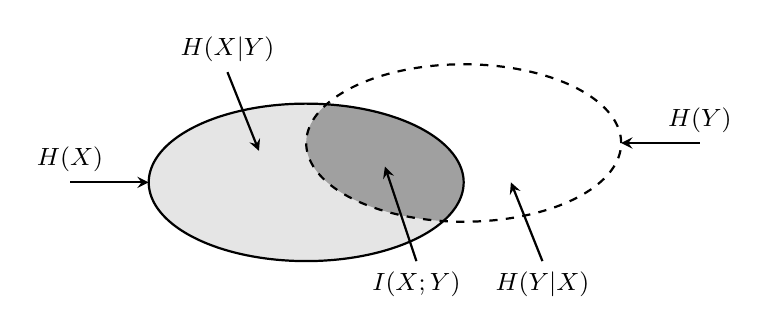
\begin{tikzpicture}[scale=2]
\shorthandoff{>}
% interior H(X) x^2 + 4 y^2 = 1 => y = \pm sqrt(1-x^2)/2
\fill[domain=0:360,samples=200,opacity=.1] plot ({cos(\x)},{.5*sin(\x)});
%
% interior H(Y) (x-1)^2 + 4 (y-1/4)^2 = 1 => y = 1/4 \pm sqrt(1-(x-1)^2)/2
% se cruzan cuando x = 1 \pm sqrt(55)/10 =>
% theta = acos(.5 \pm sqrt(55)/20) para X
% theta = acos(-.5 \pm sqrt(55)/20) para X
\pgfmathsetmacro{\s}{acos(.5-sqrt(55)/20)};
\pgfmathsetmacro{\t}{-acos(.5+sqrt(55)/20)};
\pgfmathsetmacro{\u}{-acos(-.5+sqrt(55)/20)};
\pgfmathsetmacro{\v}{acos(-.5-sqrt(55)/20)-360};
%
% interior I(X;Y)
%\draw[domain=\v:\v] plot ({cos(\x)+1},{.5*sin(\x)+.25}) node{$\bullet$};
\fill[opacity=.3]
   plot [domain=\s:\t,samples=200] ({cos(\x)},{.5*sin(\x)})
-- plot [domain=\u:\v,samples=200] ({cos(\x)+1},{.5*sin(\x)+.25})
-- cycle;
%
% borders H(X) y H(Y)
\draw[domain=0:360,samples=200,thick] plot ({cos(\x)},{.5*sin(\x)});
\draw[dashed,domain=0:360,samples=200,thick] plot ({cos(\x)+1},{.5*sin(\x)+.25});
%
% flechas y flechas condicionales
\draw[thick,>=stealth,<-] (-1,0)--(-1.5,0) node[above]{\small $H(X)$};
\draw[thick,>=stealth,<-] (-.3,.2)--(-.5,.7) node[above]{\small $H(X|Y)$};
%
\draw[thick,>=stealth,<-] (2,.25)--(2.5,.25) node[above]{\small $H(Y)$};
\draw[thick,>=stealth,<-] (1.3,0)--(1.5,-.5) node[below]{\small $H(Y|X)$};
%
\draw[thick,>=stealth,<-] (.5,.1)--(.7,-.5) node[below]{\small $I(X;Y)$};
\end{tikzpicture} \end{center}
%
\leyenda{Diagrama  de Venn: Ilustraci\'on  de la  definici\'on de  la entrop\'ia
  condicional, de la informaci\'on mutua, y de las relaciones entre cada medida.
  La superficia del  elipse en linea llena (parte grise)  representa $H(X)$ y el
  interior de la  en linea discontinua representa $H(Y)$.   La parte grise clara
  representa $H(X|Y)$  superficia del ``conjunto $H(X)$'' quitando  la parte que
  partenece  a  $H(Y)$.  La  parte  blanca  representa  $H(Y|X)$ superficia  del
  ``conjunto $H(Y)$''  quitando la  parte que partenece  a $H(X)$.  La  parte en
  grise oscuro es entonces lo que $X$ e $Y$ comparten, es decir $I(X;Y)$.}
%
\label{Fig:SZ:Venn}
\end{figure}

Como se lo va a probar, $I$ es positiva; representa realmente una informaci\'on,
la compartida  entre \ $X$  \ e  \ $Y$: Si  de la incerteza  de $X$ se  quita la
incerteza  de  $X$   una  vez  que  $Y$  es  medida,  lo   que  queda  tiene  la
significaci\'on de  la informaci\'on que  estas variables tienen en  com\'un. En
particular, de $I(X;X) = H(X)$ se denoma a veces $H(X)$ {\it auto informaci\'on}
de $X$.

Para  probar la  positividad de  $I$, se  introduce de  manera m\'as  general la
noci\'on  de  entrop\'ia  relativa,   conocida  tambi\'en  como  divergencia  de
Kullback-Leibler~\cite{KulLei51,    Kul68,    CovTho06,    Rio07}~\footnote{Esta
  divergencia fue introducida despu\'es de  la secunda guerra, en el contexto de
  la guerra  fr\'ia. Kuulback y Leibler  trabajon para la  NSA en cryptolog\'ia,
  as\'i que esta medida ncontr\'o  inicialmente aplicaciones en este macro, y el
  de la compresi\'on de datos.}:
%
\begin{definicion}[Entrop\'ia relativa]
\label{Def:SZ:entropiarelativa}
%
La entrop\'ia  relativa, o  divergencia de una  medida de probabilidad  $Q$, con
respecto a una medida de probabilidad de referencia $P$ tal que \underline{$Q \ll
  P$}, ambas definidas sobre $\Rset^d$, es definida como
  %
  \[
  \Dkl[Q]{P}  =  \int_{\Rset^d}  \frac{dQ}{dP}(x) \, \log  \left(  \frac{dQ}{dP}(x)
  \right)  \, dP(x)  = \int_{\Rset^d}  \log \left(  \frac{dQ}{dP}(x)  \right) \,
  dQ(x).
  \]
  %
  Si \  $P$ \  y \ $Q$  \ admiten una  densidad con  respecto a una  medida $\mu$
  (basicamente nos interesamos  a $\mu_L$ y $\mu_\X$), se  escribe a trav\'es de
  las  densidades  como~\footnote{En el  caso  discreto,  esta cantidad  depende
    solamente de $p$ y $q$ y no  de los estados. La condici\'on necesaria es que
    $p$ y $q$ tienen los mismos  n\'umeros de componentes (se completa el vector
    lo m\'as corto)  y si la $i$-esima componente de $q$  vale cero, entonces la
    de $p$ vale  cero tambi\'en.  Adem\'as, con $p$ y $q$  de mismo tama\~no, se
    puede poner en biyecci\'on los alfabetos  asociados a $p$ y $q$, sin perdida
    de generalidad.  En el caso  continuo, esta razonamiento no vale m\'as, esta
    cantidad dependiendo en general de los estados\ldots}
  %
 \[
 \Dkl[q]{p}  \equiv \Dkl[Q]{P}  = \int_{\Rset^d}  \log  \left( \frac{q(x)}{p(x)}
 \right) \, q(x) \, d\mu(x).
 \]
  %
\end{definicion}
%
Inicialmente, esta  medida fue  introducida por Kullback  y Leibler en  la misma
linea  que Shannon, interpretando  \ $\log\left(\frac{dQ}{dP}(x)\right)$  \ como
una informaci\'on de discriminaci\'on  entre dos hip\'otesis de distribuciones \
$Q$ \ y \  $P$ \ a partir de la observaci\'on \ $x$,  \ la divergencia siendo la
informaci\'on   de  discriminaci\'on   promedia.   Introdujeron   tambi\'en  una
versi\'on sim\'etrica, que veremos m\'as adelante.  Se notar\'a que, $\Dkl[Q]{P}
=  - \int_{\Rset^d}  q(x)  \, \log(q(x))  \,  d\mu(x) +  \int_{\Rset^d} p(x)  \,
\log(q(x)) \, d\mu(x)$.  El primer termino es nada mas que la entrop\'ia de $q$,
que se puede  ver como distribuci\'on ``presupuesta''. Menos  el secundo termino
se interpreta como el promedio de la incerteza elemental $\log(q)$ con respecto a
la distribuci\'on de referencia (``verdadera''), a veces llamado {\it entrop\'ia
  cruzada}.   Por eso,  esta divergencia  es una  entrop\'ia relativamente  a la
distribuci\'on  $p$.  En  la  misma linea,  se  puede inmediatamente  ver de  la
definici\'on general Def.~\ref{Def:SZ:ShanonMu},
%pagina~\pageref{Def:SZ:ShanonMu}, 
que  $\displaystyle  \Dkl[Q]{P} \equiv  -H\left(  \frac{dQ}{dP}  \right)$ \  con
respecto a la medida $\mu = P$.   Por ejemplo, en el caso discreto finito, si $p$
es  la   distribuci\'on  uniforme  sobre  un  alfabeto   de  cardenal  $\alpha$,
$\Dkl[q]{p} =  \log \alpha  - H(q)$,  lo que representa  una desviaci\'on  de la
entrop\'ia de  su valor  m\'aximo.  La misma  interpretaci\'on queda en  el caso
continuo con  la ley  uniforme ($p$ y  $q$ definidas  sobre el mismo  espacio de
volumen  finito) o  con la  gaussiana ($p$  y $q$  teniendo la  misma  matriz de
covarianza).  {\it Como para la  entrop\'ia, cuando se necesitar\'a un logaritmo
  especificamente de base $a$, se notar\'a la divergencia $D_{\mathrm{kl},a}$.}

\begin{lema}[Positividad de la entrop\'ia relativa]
\label{Lem:SZ:PositividadEntropiaRelativa}
%
  \[
  \Dkl[Q]{P} \ge 0 \quad \mbox{con igualdad ssi} \quad P = Q. %\quad (c.s.)
  \]
  %
\end{lema}
%
\begin{proof}
  Existen varias pruebas, pero la m\'as linda puede ser la usando la desigualdad
  de  Jensen~\footnote{En   el  caso  discreto,  se  puede   usar  tambi\'en  la
    desigualdad \ $\sum t_i \log t_i \ge  \sum t_i \log t'_i$ \ una instancia de
    la desigualdad conocida como  desigualdad log-sum, o conocida tambi\'en como
    desigualdad de  Gibbs (debido a J.  W.   Gibbs mismo)~\cite{Gib02, CovTho06,
      Rio07,         Mer10,        Mer18}.},        teorema~\ref{Teo:MP:Jensen}:
  %pagina~\pageref{Teo:MP:Jensen}:  
  para $\phi$ convexa  e \ $Y$ \ variable  aleatoria escalar, $\Esp[\phi(Y)] \ge
  \phi(\Esp[Y])$ \ con igualdad ssi \  $Y$ \ es determinista (casi siempre) si \
  $\phi$ es estrictamente  convexa.  Sea \ $X$ \ de  medida de probabilidad $P$.
  Se escribe la entrop\'ia  relativa \ $\Dkl[Q]{P} = \Esp\left[ \frac{dQ}{dP}(X)
    \log \left( \frac{dQ}{dP}(X) \right) \right]$.  Sea \ $Y = \frac{dQ}{dP}(X)$
  y  $\phi(u)  =  u  \log  u$,  funci\'on  estrictamente  convexa.   Entonces  \
  $\Dkl[Q]{P}  =  \Esp[\phi(Y)] \ge  \phi(\Esp[Y])$.   \  Pero \  $\displaystyle
  \Esp[Y]    =   \Esp\left[    \frac{dQ}{dP}(X)    \right]   =    \int_{\Rset^d}
  \frac{dQ}{dP}(x)       \,       dP(x)        =       1$       seg\'un       el
  lema~\ref{Lem:RelacionIntegracionDerivadasRadon}.
  %pagina~\pageref{Lem:RelacionIntegracionDerivadasRadon}.  \ 
  Se cierra  la prueba  con el hecho  que \  $\phi(1) = 0$  El caso  de igualdad
  apareciendo  si   y  solamente   si  \  $Y$   \  es  determinista,   es  decir
  $\frac{dP}{dQ}(X)$ \ determinista, es equivalente a \ $\frac{dP}{dQ} = 1 \quad
  (P$-c.s.)    \    (constante,   la   constante   siendo   igual    a   1   del
  lema~\ref{Lem:RelacionIntegracionDerivadasRadon} y  \ $P$ \  y \ $Q$  \ siendo
  medidas de probabilidad).
\end{proof}

Esta propiedad tiene consecuencias fijandose que
%
\[
I(X;Y) = \Dkl[P_{X,Y}]{P_X P_Y},
\]
%
\ie  la  informaci\'on  mutua  es  la  divergencia  de  Kullback-Leibler  de  la
distribuci\'on  conjunta  relativa al  producto  de  las marginales  (obviamente
$P_{X,Y} \ll  P_X P_Y$). Con este  enfoque, no se  necesita que \ $(X,Y)$  \ sea
discreta o continua admitiendo una densidad.
%
\begin{propiedades}
\item\label{Prop:SZ:Ipositive}   {\it   $I$   es   positiva,  como   medida   de
    independencia:}
  %
  \[
  I(X;Y) \ge 0 \quad \mbox{con igualdad ssi $X$ e $Y$ son independientes.}
  \]
%
\item\label{Prop:SZ:condicionar} {\it  Condicionar reduce la  entrop\'ia}
  %
  \[
  H(X|Y) \le H(X) \quad \mbox{con igualdad ssi $X$ e $Y$ son independientes.}
  \]
  %
  Esta    desigualdad,     con    la     regla    de    cadena,     prueba    la
  sub-aditividad~\ref{Prop:SZ:subaditividad}.   Esta  reducci\'on  de  incerteza
  vale en  promedio, pero el conocimiento  de un valor particular  puede ser tal
  que $H(X|Y =  y) > H(X)$, \ie \ !`un conocimiento  particular puede aumentar la
  entrop\'ia!  (ver ejemplos en~\cite[p.~59]{Rio07}).
\end{propiedades}

Fijense  que   si  $\Dkl{}$  es   positiva,  \underline{no  es   sim\'etrica}  y
\underline{tampoco  satisface la  desigualdad triangular}.  Por eso,  no  es una
distancia  y  tiene  el  nombre  de {\it  divergencia}.   La  distribuci\'on  de
referencia $P$ juega un rol fundamental.

Al  final, se mencionar\'a las propiedades adicionales siguientes:
%
\begin{enumerate}
\item $\Dkl[q]{p}$  queda invariante  bajo una misma  transformaci\'on biyectiva
  sobre  ambos $p$ y  $q$. Es  trivial en  el caso  discreto y  si no  se prueba
  sencillamente por un cambio de variables en la forma integral.
%
\item $\Dkl{}$  es convexa con respecto al  par $(P,Q)$ en el  sentido que, para
  $\pi_i \ge 0,  \: \sum_i \pi_i = 1$,  y dos conjuntos $\{ P_{(i)}  \}_i, \: \{
  Q_{(i)} \}_i$ de medidas de probabilidades tales que $Q_{(i)} \ll P_{(i)}$,
  %
  \[
  \Dkl[\sum_i   \pi_i  \ Q_{(i)}]{\sum_i   \pi_i \   P_{(i)}}  \ge   \sum_i   \pi_i
  \Dkl[Q_{(i)}]{P_{(i)}}.
  \]
  %
  La  prueba de  esta desigualdad  es dada  subsecci\'on~\ref{Ssec:SZ:Csiszar}
  %, pagina~\pageref{Ssec:SZ:Csiszar} 
  en un contexto m\'as general.
%
\item Para  $Q$ fijo, $\Dkl[Q]{P}$ es convexa  con respecto a $P$  en el sentido
  que, para $\pi_i \ge 0, \: \sum_i  \pi_i = 1$, y un conjunto $\{ P_{(i)} \}_i$
  de medidas de probabilidades tales que $Q \ll P_{(i)}$,
  %
  \[
  \Dkl[Q]{\sum_i   \pi_i \,   P_{(i)}}  \ge   \sum_i   \pi_i
  \, \Dkl[Q]{P_{(i)}}.
  \]
  %
  Eso  es  la  consecuencia  obvia  de  la concavidad  de  $u  \mapsto  \log  u$
  (escribiendo la divergencia  como densidad con respecto a  una medida dada). Es
  sencillo ver que si $\Dkl{}$ siendo convexa con respecto a $P$ ($Q$ dada) y al
  par $(P,Q)$, no puede ser convexa con respecto a $Q$ (con $P$ dada).
\end{enumerate}


% ============================== Desigualdades =============================== %

\seccion{Unas identidades y desigualdades}
\label{s:SZ:Desigualdades}

% Libro Loss Ruskai [Lieb]

\SZ{Desigualdades de Fano? Rioul p.  78, Cover P.~663, Sanov? Pythagorean? Gene:
  cf Zyc p60}

% ================================= MaxEnt

\subseccion{El principio de entrop\'ia m\'axima}
\label{sec:SZ:MaxEnt}

En  la  termodin\'amica, el  estudio  de  las caracter\'isticas  macrosc\'opicas
(din\'amica de las mol\'eculas) es prohibitivo tan el n\'umero de mol\'eculas es
importante. Por  ejemplo, un litro del  gas que respiramos  contiene $2.7 \times
10^{22}$  mol\'eculas.   De  esta  constataci\'on  se  desaroll\'o  la  f\'isica
estad\'isticas    bajo   el    impulso    de   Boltzmann~\cite{Bol96,    Bol98},
Maxwell~\cite{Max67},  Gibbs~\cite{Gib02}, Planck~\cite{Pla15} entre  otros (ver
tambi\'en~\cite[y   ref.]{Jay65,  Mer10,   Mer18}),   considerando  el   sistema
macrosc\'opico  a  trav\'es de  lo  que  llamaron  ensembles estad\'isticos:  el
sistema  global  (macrosc\'opico)  es  al equilibrio  pero  las  configuraciones
(micro-estados)  son  fluctuantes.  De  una   forma,  se  puede  asociar  a  una
configuraci\'on su  frecuencia de ocurrencia (imaginando tener  une infinidad de
copias del sistema en el  mismo estado macrosc\'opico), es decir su probabilidad
de  occurencia.   En  este  marco,  la  entrop\'ia,  describiendo  la  falta  de
informaci\'on, juega un  rol fundamental.  Un sistema sujeto  a v\'inculos, como
por  ejemplo teniendo  una energ\'ia  dada, debe  estar en  sus estado  lo m\'as
desorganizado dados  los v\'inculos.  En su  marco, se introdujo  la noci\'on de
entrop\'ia  termodin\'amica,  pero la  misma  es  tremendamente  vinculada a  la
entrop\'ia   de   Shannon   (claramente,   identificando   las   frecuencias   a
probabilidades  de ocurrencia)~\footnote{Ver  ep\'igrafe  del cap\'itulo\ldots}.
En otro terminos,  la distribuci\'on describiendo los micro-estados  debe ser de
entrop\'ia m\'axima,  dados los  v\'inculos.  Por ejemplo,  en un  gas perfecto,
donde las part\'iculas no interactuan  (aparte chocandose), la energ\'ia es dada
por las velocidades (suma de las energ\'ias cin\'eticas individuales).  Dada una
energ\'ia  fija, la  distribuci\'on  de  las velocidad  debe  ser de  entrop\'ia
m\'axima  sujeto  a  la  energ\'ia  dada  (nada m\'as  que  la  energ\'ia  va  a
``organizar''  las  configuraciones posibles).   Intuitivamente,  en un  sistema
aislado  de  $N$ part\'iculas,  las  configuraciones  van  a ser  equiprobables,
precisamente la distribuci\'on maximizando  la entrop\'ia.  \SZ{ En la secci\'on
  Sec.~\ref{sec:SZ:GasPerfecto} se va a desarollar un poco m\'as este ejemplo.}

De manera general, el problema se  formaliza como la b\'usqueda de la entrop\'ia
m\'axima  sujeto  a  v\'inculos.    Si  este  principio  naci\'o  en  mec\'anica
estad\'istica  (ver  tambi\'en~\cite{Jay57,   Jay57:2,  Jay65,  Mer10,  Mer18}),
encontr\'o  un  echo en  varios  campos:  en  inferencia bayesiana  para  elegir
distribuciones   del   a  priori~\footnote{A   partir   de  una   distribuci\'on
  parametrizada por un par\'ametro $\theta$.  El enfoque de bayesiano consiste a
  modelizar $\theta$  aleatorio, digamos $\Theta$, tal que  la distribuci\'on de
  observaciones se  escribe entonces $p_{X|\Theta}$.  Inferir  $\theta$ a partir
  de  observaciones $x$  consiste a  determinar la  distribuci\'on dicha  {\it a
    posteriori} $p_{\Theta|X}$.   Por eso,  hace falta darse  una distribuci\'on
  dicha {\it a priori} $p_\Theta$.  Si se conocen momentos por una raz\'on o una
  otra,  se  puede elegir  esta  distribuci\'on  como  la ``menos  informativa''
  posible, \ie de  entrop\'ia m\'axima dados los momentos.\label{foot:SZ:Prior}}
conociendo  unos momentos  de la  ley~\cite{Rob07, Jay68,  Jay82,  Csi91}, hacer
estimaci\'on  espectral o  de procesos  estocasticos autoregresivos~\cite{Bur67,
  Bur75,     Jay82}     o~\cite[cap.~12]{CovTho06},     entre     otros~\cite[\&
ref.]{KapKes92}.

Sea $X$ variable aleatoria viviendo  sobre $\X \subset \Rset^d$ con $K$ momentos
\  $\Esp\left[ M_k(X)  \right]  = m_k$  \ fijos,  con  $M_x: \X  \to \Rset$,  el
problema de  entrop\'ia m\'axima se  formula de la  manera siguiente en  el caso
continuo (es el caso discreto, hay que re-emplazar integrales por sumas): sean \
$M(x) = \begin{bmatrix} 1  & M_1(x) & \cdots & M_K(x) \end{bmatrix}^t$  \ y \ $m
= \begin{bmatrix} 1 & m_1 & \cdots & m_K \end{bmatrix}^t$, \ se busca,
%
\[
p^* = \argmax_p H(p) \qquad \mbox{sujeto a} \qquad p \ge 0, \quad \int_\X M(x)
\, p(x) \, dx = m
%1, \quad \int_X M_k(x) \, p(x) \, dx = m_k, \: k = 1, \ldots , K
\]
%
donde los dos primeros v\'inculos (positividad, normalizaci\'on) aseguran de que
$p^*$ sea una distribuci\'on de probabilidad. En  el ejemplo del gas, $K = 1, \,
M_1(x) = \sum_i x_i^2$ \ (los $x_i$ son las velocidades). Introduciendo factores
de   Lagrange   $\mu   =   \begin{bmatrix}    \mu_0   &   \mu_1   &   \cdots   &
  \mu_K  \end{bmatrix}^t$  para tener  en  cuenta  los  v\'inculos, el  problema
variacional   consiste  a   resolver~\cite{GelFom63,  Bru04,   Mil00,  CamMar09,
  CovTho06}
%
\[
p^* = \argmax_p \int_\X \left( - p(x) \log p(x) + \mu^t M(x) \, p(x) \right) dx
\]
%
donde  $\mu$  ser\'a  determinado  para  satisfacer a  los  v\'inculos.   De  la
ecuaci\'on  de Euler-Lagrange~\cite{GelFom63, Bru04},  esquematicamente anulando
la ``derivada''  del integrande con respeto  a $p$ (sera  realmente un gradiente
con respeto a los componentes de  $p$ en el caso discreto), reparametrizando los
factores de Lagrange, se obtiene
%
\[
p^*(x) = \e^{\mu^t M(x)}
\]
%
con $\mu$  tal que se satisfacen  los v\'inculos de  normalizaci\'on y momentos.
Esta distribuci\'on  cae en la  familia conocida como {\it  familia exponencial}
donde  los $M_k$  son  conocidos  como {\it  estad\'isticas  suficientes} y  los
$\mu_k$ {\it par\'ametros naturales}~\cite{Dar35, Koo36, And70, Kay93, LehCas98,
  Rob07}.

Un problema que  puede aparecer es que  no se puede determinar $\mu$  tal que se
satisfacen  todos los  v\'inculos,  en particular  la  de normalizaci\'on.   Por
ejemplo,  si $\X  = \Rset$  y $K  = 0$,  \ $p$  \ deber\'ia  ser  constante (ley
uniforme) sobre\ldots $\Rset$, lo que no es normalizable. De la misma manera, si
$K  =  3$  \  y  \   $M_k(x)  =  x^k$,  tampoco  es  normalizable  la  funci\'on
obtenida~\footnote{En el  enfoque Bayesiano se puede que  no sea problem\'atico,
  si el  a posteriori es normalizable~\cite{Rob07},  pero va m\'as  all\'a de la
  meta de  esta secci\'on.}.  En  otros terminos, en  este caso, el  problema no
tiene soluci\'on~\footnote{M\'as  precisamente, existen  casos en los  cuales se
  puede acotar la entrop\'ia por arriba  por un $H^{\sup}$, tal que $\sup_p H(p)
  \le H^{\sup}$ pero no  se puede alcanzar esta cota, \ie es  un supremum, no un
  m\'aximo~\cite[sec.~12.3]{CovTho06}.}.

Existe una prueba informacional de este resultado, saliendo de la soluci\'on:
%
\begin{lema}
  Sea \ $\displaystyle \P_m = \left\{ p \ge 0: \: \int_\X M_k(x) \, p^*(x) \, dx
    =  m \right\}$ \  y \  $p^* \in  \P_m$ \  que sea  de la  forma \  $p^*(x) =
  \e^{\mu^t M(x)}$. Entonces
  %
  \[
  \forall \,  p \in \P_m, \quad  H(p) \le H(p^*) \qquad  \mbox{con igualdad ssi}
  \quad p = p^*
  \]
  %
\end{lema}
\begin{proof}
  \begin{eqnarray*}
  H(p) & = & - \int_\X p(x) \, \log p(x) \, dx\\[2.5mm]
  %
  & = & - \int_\X p(x) \, \log\left( \frac{p(x)}{p^*(x)} \right) \, dx - \int_\X
  p(x) \, \log p^*(x) \, dx
  \end{eqnarray*}
  %
  De $\log p^* = \mu^t M$ se obtiene
  %
  \begin{eqnarray*}
  H(p) & = & - \Dkl[p]{p^*} - \int_\X \mu^t M(x) p(x)
  \, dx\\[2.5mm]
  %
  & = & - \Dkl[p]{p^*} - \int_\X \mu^t M(x) \, p^*(x) \, dx\\[2.5mm]
  %
  & = & - \Dkl[p]{p^*} - \int_\X p^*(x) \log p^*(x) \, dx\\[2.5mm]
  %
  & = & - \Dkl[p]{p^*} + H(p^*)
  \end{eqnarray*}
  %
  porque $p,  p^* \in  \P_m$ \ y  \ $\mu^t M  = \log  p^*$. La prueba  se cierra
  notando que $\Dkl[p]{p^*} \ge 0$ con igualdad si y solamente si $p = p^*$.
\end{proof}
%
Este lema prueba que, dados  v\'inculos ``razonables'', la entrop\'ia es acotada
por  arriba, y que  se alcanza  la cota  para una  distribuci\'on de  la familia
exponencial. Por ejemplo,
%
\begin{itemize}
\item Con  $K =  0$ \  y \  $\X$ \ de  volumen finito  \ $|\X|  < +  \infty$, la
  distribuci\'on  de entrop\'ia  m\'axima es  la distribuci\'on  uniforme  de la
  propiedad~\ref{prop:SZ:cotamaximauniforme}      \     de      la     secci\'on
  Sec.~\ref{sec:SZ:Diferencial}      en       el      caso      continuo,      o
  propiedad~\ref{prop:SZ:cotamaxima}        \       de        la       secci\'on
  Sec.~\ref{sec:SZ:DefinicionShannon} en el caso discreto.
%
\item Con  $K =  1$, \ $\X  = \Rset^d$  \ y \  $M(x) = x  x^t$ (visto  con $d^2$
  v\'inculos),  la distribuci\'on  de entrop\'ia  m\'axima es  la distribuci\'on
  gausiana de  la propiedad~\ref{prop:SZ:cotamaximagaussiana} \  de la secci\'on
  Sec.~\ref{sec:SZ:Diferencial}.
\end{itemize}


% ================================= EPI

\subseccion{Desigualdad de la potencia entr\'opica}

Sean  $X$ e  $Y$  dos variables  independientes.   Si se  conoce las  relaciones
vinculando \  $H(X,Y)$, \  $H(X)$, \ $H(Y)$,  una pregunta natural  concierna la
relaci\'on  que podr\'ia  tener \  $X+Y$  \ con  cada variable  en t\'ermino  de
entrop\'ia. La respuesta no es trivial, y el resultado general concierna el caso
de  variables continuas  sobre $\Rset^d$.   Es conocido  como desigualdad  de la
potencia entr\'opica (EPI para entropy power inequality en ingl\'es). No vincula
las entrop\'ias, sino que las potencias entr\'opicas.
%
\begin{teorema}[Desigualdad de la potencia entr\'opica]
  Sean  $X$  e $Y$  dos  variables  $d$-dimensionales continuas  independientes
  Entonces
  %
  \[
  N(X + Y) \ge N(X) + N(Y)
  \]
%
  con igualdad si y  solamente si \ $X$ \ e \ $Y$  \ son gaussianas con matrices
  de covarianza proporcionales, $\Sigma_Y \propto \Sigma_X$
  % (siempre  verdad en  el contexto  escalar).
\end{teorema}
%
\noindent     Existen    varias     formulaciones     alternativas    a     esta
desiguladad~\cite{Sha48, Lie78, CovTho06, DemCov91, Rio07}:
%
\begin{enumerate}
\item\label{EPI:SZ:EquivGauss} Sean  \ $\widetilde{X}$  \ y \  $\widetilde{Y}$ \
  gaussianas independientes  de matrices de covarianza proporcionales  y tal que
  $H(\widetilde{X}) = H(X)$ y $H(\widetilde{Y}) = H(Y)$.  Entonces
  %
  \[
  N(X+Y) \ge N\left( \widetilde{X} + \widetilde{Y} \right)
  \]
  %
  con igualdad si y solamente si \ $X$ \ y \ $Y$ \ son gaussianas.
%
\item\label{EPI:SZ:PresCov}    {\it    Desigualdad    de    preservaci\'on    de
    covarianza:}
  %
  \[
  \forall  \:   0  \le  \mu  \le   1,  \quad  H\left(   \sqrt{\mu}  X  +
    \sqrt{1-\mu} Y \right) \ge \mu H(X) + (1-\mu) H(Y)
  \]
  %
  con igualdad si y solmente si \ $X$ \ e \ $Y$ \ son gaussianas con matrices de
  covarianza proporcionales.
\end{enumerate}
%

La  prueba  de  esta(s)  desigualdad(es)  no es  trivial.   N\'umeras  versiones
existen,  dadas por  ejemplo  en las  referencias~\cite{Bla65, Sta59,  ShaWea64,
  Rio07,  Rio11,  Rio17,  CovTho06,  DemCov91,  Lie78,  VerGuo06}  (ver  tambien
teorema~6 de~\cite{Lie75}).   Como se  lo puede ver,  la gaussiana juega  un rol
particular en esta desigualdad, saturandola.


\SZ{Ver si  es corto probar  la equivalencia entre  las tres formas.  Existe una
  forma, de Madiman, a traver rearreglo}

Una gracia de la desigualdad de la potencia entr\'opica es que puede dar lugar a
pruebas  informacionales  de  desigualdades  matriciales, como  por  ejemplo  la
desigualdad  de Minkowsky  de los  determinentes  \ $|R_1  + R_2|^{\frac1d}  \ge
|R_1|^{\frac1d}  +  |R_2|^{\frac1d}$  \  para cualquieras  matrices  $R_1,  R_2$
sim\'etricas definidas  positivas, con igualdad  si y solamente si  $R_2 \propto
R_1$  (viene de  $X$ e  $Y$ gaussianas  de covarianza  $R_1$ y  $R_2$).  Aparece
tambi\'en  para acotar  la informaci\'on  mutua  entre variables  y calcular  la
capacidad  de   un  canal  de  comunicaci\'on   como  se  lo  va   a  ver  m\'as
adelante~\cite{CovTho06, DemCov91, Rio07, Joh04}.

\SZ{En el caso discreto, no hay un resultado general.  Existen solamente 
  resultados para variables particulares~\cite{toto, titi}.}


% ================================= Data Processing Theorem

\subseccion{Desigualdad de procesamiento de datos}

Esta  desigualdad  traduce  que  procesando  datos,  no  se  puede  aumentar  la
informaci\'on disponible sobre  una variable. Se basa sobre  una desigualdad que
satisface la informaci\'on mutua aplicada a un proceso de Markov.

\begin{definicion}[Proceso de Markov]
  Una secuencia  $X_1 \mapsto X_2 \mapsto  \ldots \mapsto X_n$ es  dicha {\it de
    Markov}   si   para  cualquier \   $i   >   1$,
  %
  \[
  p_{X_{i-1},X_{i+1}|X_i} = p_{X_{i-1}|X_i} \, p_{x_{i+1}|X_i}
  \]
  %
  Dicho de otra manera, condicionalmente a  \ $X_i$, las variables \ $X_{i-1}$ \
  y \ $X_{i+1}$ son independientes.  Eso es equivalente a
  %
  \[
  p_{X_{i+1}|X_i,X_{i-1},\ldots} = p_{X_{i+1}|X_i}
  \]
  %
  Si  $i$ representa  un tiempo,  significa  que la  estad\'istica de  $X_{i+1}$
  conociendo todo el pasado se reduce  a esa conociendo el pasado inmediato (las
  probabilidades   dichas   de   transici\'on   $p_{X_{i+1}|X_i}$   caracterizan
  completamente el  proceso).  Es sencillo  fijarse de que $X_n  \mapsto X_{n-1}
  \mapsto \ldots \mapsto X_1$ es tambien un proceso de Markov.
\end{definicion}

\begin{teorema}[Desigualdad de procesamiento de datos]
  Sea  $X \mapsto  Y \mapsto  Z$ un  proceso de  Markov. Entonces,
  %
  \[
  I(X;Y) \ge I(X;Z)
  \]
  %
  con igualdad si y solamente si $X \mapsto Z \mapsto Y$ es tambi\'en un proceso
  de Markov. En  particular, es sencillo ver que  para cualquiera funci\'on $g$,
  $X \mapsto Y \mapsto g(Y)$ es un proceso de Markov, lo que da
  %
  \[
  \forall \, g, \quad I(X;Y) \ge I(X;g(Y))
  \]
  %
  La  \'ultima  desigualdad  se  escribe  tambi\'en  $H(X|g(Y))  \ge  H(X|Y)$  y
  significa que  procesar $Y$ no aumenta  la informaci\'on que $Y$  da sobre $X$
  (la incerteza condicional es m\'as importante).
\end{teorema}
%
\begin{proof}
  Por definici\'on  de la  informaci\'on mutua, considerando  $X$ y  la variable
  conjunta $(Y,Z)$,
  %
  \begin{eqnarray*}
  I(X ; Y,Z) & = & H(X) - H(X|Y,Z)\\[2.5mm]
  %
  & = & H(X) - H(X|Y) + H(X|Y) - H(X|Y,Z)
  \end{eqnarray*}
  %
  \noindent  Por la  propiedad que  $Z  \mapsto Y  \mapsto X$  sea tambi\'en  un
  proceso de Markov,  es sencillo probar que $H(X|Y,Z)  = H(X|Y)$ (conciendo $Y$
  sufice para caracterizar completamente $X$), lo que da
  %
  \[
  I(X;Y,Z) = I(X;Y)
  \]
  %
  Tambi\'en,
  %
  \begin{eqnarray*}
  I(X ; Y,Z) & = & H(X) - H(X|Z) + H(X|Z) - H(X|Y,Z)\\[2.5mm]
  %
  & = & I(X;Z) + H(X|Z) - H(X|Y,Z)
  \end{eqnarray*}
  %
  \noindent  Adem\'as, escribiendo $\frac{p_{X|Y,Z}}{p_{X|Z}}  = \frac{p_{X|Y,Z}
    \, p_{Y|Z}}{p_{X|Z} p_{Y|Z}} = \frac{p_{X,Y|Z}}{p_{X|Z} p_{Y|Z}}$ se nota de
  que  \ $H(X|Z)  -  H(X|Y,Z)$ \  es  la divergencia  de  Kullback-Leibler de  \
  $p_{X,Y|Z}$ \  relativamente a  \ $p_{X|Z} p_{Y|Z}$,  o informaci\'on  mutua \
  $I(X;Y|Z)$ entre \ $X$ \ e \  $Y$, condicionalmente a \ $Z$.  Entonces, de las
  dos formas de $H(X;Y,Z)$ viene
  %
  \[
  I(X;Y) = I(X;Z) + I(X;Y|Z)
  \]
  %
  La desigualdad del teorema viene de la positividad de $I(X;Y|Z)$. Adem\'as, se
  obtiene la igualdad si  y solamente si \ $I(X;Y|Z) = 0$, es decir  \ $X$ \ e \
  $Y$ \  independientes condicionalmente a \  $Z$, lo que es  la definici\'on de
  que $X \mapsto Z \mapsto Y$ sea un proceso de Markov.
\end{proof}

% ================================= Data Processing Theorem

\subseccion{Segunda ley de la termodin\'amica}

Tratando de procesos  de Markov, aparece el equivalente de la  segunda ley de la
termodin\'amica:  un sistema  aislado evolua  hasta  llegar su  estado lo  m\'as
desorganizado (ver ej.~\cite[y ref.]{CovTho06, Mer10, Mer18}).

\begin{lema}[Versi\'on informacional de la segunda ley de la termodin\'amica]
  Sea $X_1 \mapsto X_2 \mapsto \cdots  \mapsto X_n \mapsto \cdots$ un proceso de
  Markov,  con probabilidades  de transici\'on  $p_{X_{n+1}|X_n}$  dadas.  Estas
  \'ultimas modelizan  el sistema,  independiente de las  condiciones iniciales.
  Sean  dos  distribuciones   (condiciones)  iniciales  diferentes  $p_{(1)}$  y
  $q_{(1)}$,  conduciendo  a  las  distribuciones  $p_{(n)}$  y  $q_{(n)}$  para
  $X_n$. Entonces:
%
\begin{itemize}
\item  Para cualquier  $n \ge  1$,
  %
  \[
  \Dkl[p_{(n+1)}]{q_{(n+1)}} \le \Dkl[p_{(n)}]{q_{(n)}}
  \]
  %
  las  distribuciones   $p_{(n)}$  y  $q_{(n)}$  no  se   ``alejan''  (tiende  a
  acercarse);
%
\item  Si  $p^*$  es  una  distribuci\'on  estacionaria,
  %
  \[
  \Dkl[p_{(n+1)}]{p^*} \le \Dkl[p_{(n)}]{p^*}
  \]
  %
  la distribuci\'on no se aleja de la distribuci\'on estacionaria.
%
\item Adem\'as, si  los $X_n$ tienen $K$ momentos fijos  $m = \Esp[M(X_n)] \quad
  \forall \,  n$ y si $p^*$  es la distribuci\'on de  entrop\'ia m\'axima tiendo
  los mismos momentos como  descrito secci\'on Sec.~\ref{sec:SZ:MaxEnt}, (ej. $K
  = 0$,  $\X$ de cardinal o  volumen finito y ley  uniforme, $K =  2$, $T_k(x) =
  x^k$ y ley gausiana),
  %
  \[
  H(X_{n+1}) \ge H(X_n)
  \]
  %
  el  sistema   tiende  a  desorganizarse (dando los vinculos/momentos).
\end{itemize}
\end{lema}
%
\begin{proof}
  Escribiendo  \ $p_{(n+1),(n)}$  \  y \  $q_{(n+1),(n)}$  \ las  distribuciones
  conjuntas  de  $(X_{n+1},X_n)$  \   para  las  dos  condiciones  iniciales,  \
  $p_{(n+1)|(n)}$ \ y \ $q_{(n+1)|(n)}$  \ las distribuciones condicionales de \
  $X_{n+1}|X_n$  \  as\'i  que  $p_{(n)|(n+1)}$  \ y  \  $q_{(n)|(n+1)}$  \  las
  distribuciones condicionales de \  $X_n|X_{n+1}$, se muestra sencillamente que
  \          $\displaystyle         \Dkl[p_{(n+1),(n)}]{q_{(n+1),(n)}}         =
  \Dkl[p_{(n+1)}]{q_{(n+1)}}                        +                       \int
  \Dkl[p_{(n)|(n+1)}(\cdot,y)]{q_{(n)|(n+1)}(\cdot,y)}            dy           =
  \Dkl[p_{(n)}]{q_{(n)}}                          +                         \int
  \Dkl[p_{(n+1)|(n)}(\cdot,y)]{q_{(n+1)|(n+1)}(\cdot,y)} dy$  \ (y con  una suma
  en  lugar de la  integral en  el caso  discreto).  Adem\'as,  $p_{(n+1)|(n)} =
  p_{X_{n+1}|X_n}         =         q_{(n+1)|(n)}$,        conduciendo         a
  $\Dkl[p_{(n+1)|(n)}(\cdot,y)]{q_{(n+1)|(n)}(\cdot,y)} =  0$ \ con consecuencia
  de que \  $\displaystyle \Dkl[p_{(n)}]{q_{(n)}} = \Dkl[p_{(n+1)}]{q_{(n+1)}} +
  \int      \Dkl[p_{(n)|(n+1)}(\cdot,y)]{q_{(n)|(n+1)}(\cdot,y)}     dy$.      \
  $p_{(n)|(n+1)}$  no  es necesariamente  igual  a  \  $q_{(n)|(n+1)}$, pero  la
  divergencia siendo no negativa, se obtiene la primera desigualdad.  La segunda
  desigualdad se obtiene  tomando \ $q_{(n)} = p^*$.  Adem\'as, si  \ $p^*$ \ es
  le entrop\'ia  m\'axima de mismos momentos  $m = \Esp[M(X_n)]$  que los $X_n$,
  hemos  visto  de  que  \  $p^*(x)  =  \e{\mu^t M(x)}$  \  ley  de  la  familia
  exponencial, dando \  $\Dkl[p_{(n)}]{p^*} = -H(X_n) - \mu^t  m$, conduciendo a
  la \'ultima desigualdad.
\end{proof}


% ================================= Principop de incerteza

\subseccion{\SZ{Principio de incerteza entr\'opico}}

\SZ{Bourret 58, Leipnik 59 entre otros que ya citamos un par de veces}

% ================================= Fisher

\subseccion{Un foco sobre la informaci\'on de Fisher}

Si la  entrop\'ia y las heramientas  relacionadas son naturales  como medidas de
informaci\'on, no se  puede resumir una distribuci\'on a  una medida escalar. En
el marco de la teor\'ia de  la estimaci\'on, R. Fisher introdujo una noci\'on de
informaci\'on intimamente  relacionada al error cuadr\'atico  en la estimaci\'on
de   un  par\'ametro   a  partir   de  una   variable  parametrizado   por  este
par\'ametro~\cite{Fis22, Fis25:07, Kay93, Bos07, CovTho06, Fri04}.

{\it Mencionamos que en esta secci\'on, se usar\'a el logaritmo natural.}
% , a pesar de que sea  necesarion solamente para la desigualdad de Cram\'er-Rao
% que se va a ver en unos parafos.}
%
\begin{definicion}[Matriz informaci\'on de Fisher par\'ametrica]
  Sea   $X$   una   variable   aleatoria  parametrizada   por   un   par\'ametro
  $m$-dimensional, $\theta  \in \Theta \subseteq \Rset^m$,  de distribuci\'on de
  probabilidad  $p_X(\cdot;\theta)$  continua sobre  $\X  \subseteq \Rset^d$  su
  soporte. Suponga que  $p_X$ sea diferenciable en $\theta$  sobre $\Theta$.  La
  matriz de Fisher, de tama\~no $m \times m$, es definida por
  %
  \[
  J_\theta(X)  =  \Esp\left[  \Big(  \nabla_\theta \log  p_X(X;\theta)  \Big)
    \Big( \nabla_\theta \log p_X(X;\theta) \Big)^t \right]
  \]
  %
  donde \  $\nabla_\theta = \left[ \cdots  \: \frac{\partial}{\partial \theta_i}
    \:  \cdots \right]^t$ \  es el  gradiente en  \ $\theta$.   Es la  matriz de
  covarianza  del  {\it  score  param\'etrico}  \  $S(X)  =  \nabla_\theta  \log
  p_X(X;\theta)$ \  (se prueba  de que su  promedio es  igual a cero),  siendo \
  $\log p_X$ \ la {\it  log-verosimilitud}.  Bajo condiciones de regularidad, se
  puede  mostrar~\footnote{Es una  consecuencia del  teorema de  la divergencia,
    suponiendo que los bordes del soporte \ $\X$ \ no dependen de \ $\theta$ \ y
    que la funci\'on  score se cancela en estos bordes.}   que \ $J_\theta(X)$ \
  vale tambi\'en menos  el promedio de la Hessiana~\footnote{Para  \ $f: \Rset^m
    \mapsto  \Rset,  \quad \Hess_\theta  f$  \ es  la  matriz  de componentes  \
    $\frac{\partial^2 f}{\partial \theta_i \partial \theta_j}$.}  $\Hess_\theta$
  \ de  \ $\log  p_X(X;\theta)$.  Nota:  a veces se  define la  informaci\'on de
  Fisher como $\Tr(J)$, traza de la matriz informaci\'on de Fisher.
\end{definicion}
%
Como  para  la  entrop\'ia,  la  matriz  de Fisher  se  escribe  generalmente  \
$J_\theta(X)$, \ a pesar de que no sea  funci\'on de \ $X$ \ pero de la densidad
de  probabilidad.  Se  la  notar\'a  tambi\'en \  $J_\theta(p_X)$  \ seg\'un  la
escritura la m\'as conveniente.

Tomando  el gradiente  en \  $x$ \  en lugar  de \  $\theta$ \  da la  matriz de
informaci\'on de Fisher no param\'etrica,
%
\begin{definicion}[Matriz informaci\'on de Fisher no param\'etrica]
  Sea \ $X$ \ una variable aleatoria de distribuci\'on de probabilidad \ $p_X$ \
  definida sobre \  $\X \subseteq \Rset^d$ \ su soporte.  Suponga  que \ $p_X$ \
  sea diferenciable (en \ $x$).  La matriz de Fisher no param\'etrica, $d \times
  d$, es definida por
  %
  \[
  J(X) =  \Esp\left[ \Big(  \nabla_x \log p_X(X)  \Big) \Big(  \nabla_x \log
      p_X(X) \Big)^t \right]
  \]
  %
  Es  la matriz  de covarianza  de  la {\it  funci\'on score}  \ $\nabla_x  \log
  p_X(X)$ \ (se prueba que su  promedio tambi\'en vale cero) o, bajo condiciones
  de  regularidad,  menos  el  promedio  de  la  Hessiana  en  \  $x$  \  de  la
  log-verosimilitud.
\end{definicion}
%
Es interesante notar que:
%
\begin{itemize}
\item Cuando  \ $\theta$ \ es  un par\'ametro de posici\'on,  \ $p_X(x;\theta) =
  p(x - \theta)$, \ $\nabla_\theta \log p_X  = - \nabla_x \log p_X$ \ tal que la
  informaci\'on param\'etrica se reduce a la informaci\'on no param\'etrica.
%
\item Si \ $X$ \ es gaussiano  de matriz de covarianza \ $\Sigma_X$, entonces se
  muestra sencillamente  de que  \ $J(X)  = \Sigma_X^{-1}$ \  (o, de  una forma,
  inversa de la dispersi\'on o incerteza en t\'ermino de estad\'isticas de orden
  2).
%
\item Es sencillo ver  que, por definici\'on \ $J_\theta(X)$ \ y  \ $J(X)$ \ son
  sim\'etricas  y que  \ $J_\theta(X)  >  0$ \  y \  $J(X)  > 0$  \ donde  estas
  desiguladades  significan  que  las  matrices  son  definidas  positivas  (los
  autovalores son positivos).  Adem\'as,
  %
  \[
  \forall \ a \ne 0, \quad J(aX) = \frac{1}{|a|^2} J(X)
  \]
  %
  (queda v\'alido para $a$ matriz invertible).   Esta relaci\'on da a \ $J(X)$ \
  un sabor  de informaci\'on  en el  sentido de que,  cuando \  $a$ \  tiende al
  infinito, \ $J(aX)$ \ tiende a 0; \  $a X$ \ tiende a ser muy dispersada as\'i
  que no hay informaci\'on sobre su posici\'on.
%
\item $J_\theta$ \  y \ $J$ \ son  convexas en el sentido de  que para cualquier
  conjunto de \ $\pi_k \ge 0, \, \sum_{k=1}^K \pi_k = 1$ \ y \ cualquier
  conjunto de distribuciones \ $p_{(k)}, \ k = 1, \ldots , K$~\cite{Coh68, Fri04},
  %
  \[
  J_\theta\left(  \sum_{k=1}^K  \pi_k  p_{(k)}  \right)  \:  <  \:  \sum_{k=1}^K
  \pi_k  \,  J_\theta\left(  p_{(k)}  \right)  \qquad  \mbox{y}  \qquad  J\left(
    \sum_{k=1}^K \pi_k  p_{(k)} \right) \:  < \: \sum_{k=1}^K  \pi_k J\left(
    p_{(k)} \right)
  \]
  %
  donde $A < B$ significa que $B-A$ es definida positiva.  La prueba es dada por
  Cohen en  el caso  escalar, pero se  extiende sin  costo adicional en  el caso
  multivariado.   Hace falta  probarlo para  \ $K=2$  \ y,  por  recurrencia, se
  extiende para  cualquier \ $K$. En  este caso, observando que  \ $\big( \nabla
  \log p  \big) \big( \nabla \log  p \big)^t \,  p = \frac{\big( \nabla  p \big)
    \big(  \nabla p  \big)^t}{p}$, considerando  el  gradiente con  respeto a  \
  $\theta$ (resp. a \ $x$) tratando de  \ $J_\theta$ (resp. \ $J$), se obtiene \
  $\sum_k  \pi_k   \frac{\big(  \nabla   p_{(k)}  \big)  \big(   \nabla  p_{(k)}
    \big)^t}{p_{(k)}} - \frac{\left( \nabla  \sum_k \pi_k p_{(k)} \right) \left(
      \nabla   \sum_k   \pi_k  p_{(k)}   \right)^t}{\sum_k   \pi_k  p_{(k)}}   =
  \frac{1}{\sum_k   \pi_k    p_{(k)}}   \,   \sum_{k,l}    \pi_k   \pi_l   \Big(
  \frac{p_l}{p_{(k)}} \big( \nabla p_{(k)}  \big) \big( \nabla p_{(k)} \big)^t -
  \big(  \nabla p_{(k)}  \big) \big(  \nabla p_l  \big)^t \Big)$,  lo  que vale,
  tratando  del caso  $K =  2$, \  $ \frac{\pi_1  \pi_2}{p_{(2)}  p_{(2)} (\pi_1
    p_{(1)}  + \pi_2  p_{(2)})} \big(  p_{(2)} \nabla  p_{(1)} -  p_{(1)} \nabla
  p_{(2)} \big)  \big( p_{(2)} \nabla  p_{(1)} - p_{(1)} \nabla  p_{(2)} \big)^t
  \ge 0$.  No puede ser id\'enticamente cero (salvo si \ $\pi_1 \pi_2 = 0$ \ o \
  $p_{(1)} = p_{(2)}$\ldots) as\'i que se obtiene la desigualdad sobre la matriz
  de Fisher integrando esta \'ultima desigualdad.
\end{itemize}


Una  otra  interpretaci\'on  de \  $J$  \  como  informaci\'on  es debido  a  la
desigualdad   de   Cram\'er-Rao   que   la   relaciona  a   la   covarianza   de
estimaci\'on~\footnote{De hecho, pareci\'o esta formula tambi\'en en los papeles
  de  Fr\'echet y  de Darmois~\cite{Fre43,  Dar45}. Como  citado  por Fr\'echet,
  aparece que la primera versi\'on de esta formula es mucho m\'as vieja y debido
  a K.  Pearson  \& L. N.  G Filon~\cite{PeaFil98} en  1898; luego fue extendida
  por          Edgeworth~\cite{Edg08},          Fisher~\cite{Fis25:07}         o
  Doob~\cite{Doo36}.}~\cite{Rao45,  Rao92,  RaoWis47,  Cra46,  Rio07,  CovTho06,
  Fri04, Kay93,  Bos07}.  Sea \  $X$ \ parametrizada  por $\theta$.  La  meta es
estimar \ $\theta$  \ a partir de \  $X$.  Tal estimador va a  ser una funci\'on
\'unicamente de  \ $X$, lo  que se escribe usualmente~\footnote{Por  ejemplo, si
  $\theta$  es  un promedio  com\'un  a los  componentes  de  $X$, un  estimador
  podr\'ia    ser    \     $\widehat{\theta}    =    \frac1d    \sum_i    X_i$.}
$\widehat{\theta}(X)$ \ (la funci\'on  no depende expl\'icitamente de $\theta$).
Las caracter\'isticas de  la calidad de un estimator es  naturalmente su sesgo \
$b(\theta) = \Esp\left[  \widehat{\theta}(X) \right] - \theta$ \  y su matriz de
covarianza  \  $\Sigma_{\widehat{\theta}}$ \  (la  varianza  da la  dispersi\'on
alrededor de su promedio).  La desigualdad de Cram\'er-Rao acota por debajo esta
covarianza.
%
\begin{teorema}[Desigualdad de Cram\'er-Rao]
  Sea  \ $X$  \  parametrizada por  \ $\theta$,  de  densidad de  soporte \  $\X
  \subseteq \Rset^d$ \ indendiente de  \ $\theta$, \ y \ $\widehat{\theta}(X)$ \
  un  estimador   de  \   $\theta$.   Sea   \  $b(\theta)$  \   su  sesgo   y  \
  $\Sigma_{\widehat{\theta}}$ \ su matriz de covarianza.  Sea \ $\Jac_b(\theta)$
  \ la matriz Jacobiana del sesgo \ $b$.  Entonces,
  %
  \[
  \Sigma_{\widehat{\theta}} - \left( I + \Jac_b(\theta) \right) J_\theta(X)^{-1}
  \left( I + \Jac_b(\theta) \right)^t \ge 0
  \]
  %
  En particular, en el  caso \ $\theta$ \ escalar,
  %
  \[
  \sigma_{\widehat{\theta}}^2 \ge \frac{(1+b'(\theta))^2}{J_\theta(X)}
  \]
  %
  donde  \  $b'$ \  es  la  derivada de  \  $b$.\newline  Tomando  \ $\theta$  \
  par\'ametro de posici\'on y \  $\widehat{\theta} = X$, estimador sin sesgo ($b
  =  0$),  da  lo que  es  conocido  como  la  desigualdad no  param\'etrica  de
  Cram\'er-Rao y toma la expresi\'on
  %
  \[
  \Sigma_X - J(X)^{-1} \ge 0
  \]
  %
  o, en el caso escalar,
  %
  \[
  \sigma_X^2 \ge \frac{1}{J(X)}
  \]
  %
  Adem\'as, en el caso no param\'etrico, se  alcanza la cota si y solamente si \
  $X$ \ es un vector gaussiano.
\end{teorema}
%
\noindent Esta desigualdad  acota la varianza de cualquier  estimador, \ie da la
varianza o error m\'inimo(a) que se puede esperar. Esta cota es el inverso de la
informaci\'on de Fisher, \ie \  $J_\theta(X)$ \ caracteriza la informaci\'on que
\ $X$ \ tiene sobre \ $\theta$.
%
\begin{proof}
  Sea  \   $S  =  \nabla_\theta  \log   p_X$  \  y  \   $\theta_0  =  \Esp\left[
    \widehat{\theta}(X)  \right]   =  \theta  +  b(\theta)$.   Fijandose  que  \
  $\nabla_\theta \log p_X \, p_X  = \nabla_\theta p_X$, que \ $\widehat{\theta}$
  \ no  es funci\'on de \ $\theta$,  y que el soporte  \ $\X$ \ no  depende de \
  $\theta$,  se   obtiene~\footnote{Se  supone   que  los  integrandes   sean  \
    $\theta$-localmente  integrables, tal que  se puede  invertir derivada  en \
    $\theta$ \ e integraci\'on.}
  %
  \begin{eqnarray*}
  \Esp\left[ S(X) \left( \widehat{\theta}(X) - \theta_0 \right)^t \right] & = &
  \int_\X \nabla_\theta p_X(x;\theta) \widehat{\theta}(x)^t \, dx - \left(
  \int_\X \nabla_\theta p_X(x;\theta) \, dx \right) \theta_0^t\\[2.5mm]
  %
  & = & \nabla_\theta \int_{\Rset^d} p_X(x;\theta) \widehat{\theta}(x)^t \, dx -
  \left( \nabla_\theta \int_{\Rset^d} p_X(x;\theta) \, dx \right)
  \theta_0^t\\[2.5mm]
  %
  & = & \nabla_\theta \left( \theta + b(\theta) \right)  - 
  \left( \nabla_\theta 1 \right) \theta_0^t\\[2.5mm]
  %
  & = & \left( I + \Jac_b(\theta) \right)^t
  \end{eqnarray*}
  %
  Adem\'as, fijandose  que \  $\Esp\left[ S(X) S(X)^t  \right] =  J_\theta(X)$ y
  $\Esp\left[   \left(    \widehat{\theta}(X)   -   \theta_0    \right)   \left(
      \widehat{\theta}(X)      -      \theta_0      \right)^t     \right]      =
  \Sigma_{\widehat{\theta}}$,            la            desigualdad            de
  Cauchy-Bunyakovsky-Schwarz~\footnote{De  hecho, fue  probada  por Cauchy  para
    sumas en  1821, para integrales por  Bunyakovsky en 1859  y m\'as elegamente
    por Schwarz en 1888~\cite{Ste04}.}  conduce a
  %
  \[
  \left( u^t \left( I + \Jac_b(\theta)  \right)^t v \right)^2 \: = \: \Esp\left[
    u^t S(X) \left( \widehat{\theta}(X) -  \theta_0 \right)^t v \right]^2 \: \le
  \: u^t J_\theta(X) u \: v^t \Sigma_{\widehat{\theta}} \, v
  \]
  %
  La prueba se termina tomando \ $u = J_\theta(X)^{-1} \left( I + \Jac_b(\theta)
  \right)^t \,  v$ \ (recordandose que  \ $J$ \ es  sim\'etrica).\newline Con la
  elecci\'on  de \  $u$,  en la  desigualdad  de Cauchy-Bunyakovsky-Schwarz,  se
  obtiene la igualdad  cuando \ $v^t J(X)^{-1} S(x) \propto v^t  (x - \theta)$ \
  para cualquier \ $v$ \ y \ $x$,  est decir \ $\nabla_x p_X (x) \propto J(X) (x
  -  \theta)  p_X(x)$,  lo  que  es  la  ecuaci\'on  diferencial  que  satisface
  (solamente) la gaussiana: en este caso, se verifica a posteriori que \ $J(X) =
  \Sigma_X^{-1}$,  y  entonces que  se  alcanza la  cota  de  la desigualdad  de
  Cram\'er-Rao no param\'etrica.
\end{proof}
%
\noindent En el caso param\'etrico, no se puede estudiar el caso de igualdad del
hecho de  que \ $\widehat{\theta}$ \ no  es algo dado.  Adem\'as,  a\'un dado un
estimador (expl\'icitamente independiente de $\theta$), no hay garant\'ia de que
existe una  densidad parametrizada por  \ $\theta$ \  que alcanza la cota,  o al
rev\'es, dada  una familia de densidades,  tampoco hay garant\'ia  que existe un
estimador que permite alcanzar la cota~\cite{CovTho06, Kay93}.

Fijense  de  que,  nuevamente,  la  gaussiana  juega un  rol  particular  en  la
desigualdad de Cram\'er-Rao no param\'etrica, permitiendo de alcanzar la cota.

Nota: para  dos matrices \  $A \ge 0$  \ y \  $B \ge 0$,  si \ $A  - B \ge  0$ \
entonces $|A| \ge  |B|$, con igualdad si y solamente si  \ $A = B$~\cite[cap.~1,
teorema~25]{MagNeu99}.   Entonces,  de  las  desigualdades  de  Cram\'er-Rao  se
deducen desigualdades de Cram\'er-Rao escalares
%
\[
\left|   \Sigma_{\widehat{\theta}}  \right|   \,   \ge  \,   \frac{\left|  I   +
    \Jac_b(\theta) \right|^2}{\left| J_\theta(X) \right|} \qquad \mbox{y} \qquad
\left| \Sigma_X \right| \, \ge \, \frac{1}{\left| J(X) \right|}
\]
%
Obviamente, en la segunda,  se alcanza la igualdad si y solamente  si \ $X$ \ es
gaussiano.   Adem\'as, para  una  matriz \  $A  \ge 0$,  existe la  ``relaci\'on
determinente-traza''  \ $|A|^{\frac1d} \le  \frac1d \Tr(A)$,  con igualdad  si y
solamente si  \ $A = I$~\cite[cap.~11, sec.~4]{MagNeu99},  dando otras versiones
escalares de la desigualdad de Cram\'er-Rao, por ejemplo
% \Tr\left(\Sigma_{\widehat{\theta}}  \right)  \,  \ge  \, \frac{d^2  \,  \left(
%     \Tr\left(I   +  \Jac_b(\theta)  \right)   \right)^2}{\Trleft|  J_\theta(X)
% \right|} \qquad \mbox{y} \qquad
%
\[
\left| \Sigma_X  \right|^{\frac1d} \,  \ge \, \frac{d}{\Tr\left(  J(X) \right)},
\qquad   \Tr\left(   \Sigma_X   \right)   \,   \ge   \,   \frac{d}{\left|   J(X)
  \right|^{\frac1d}} \qquad \mbox{o} \qquad \Tr\left( \Sigma_X \right) \, \ge \,
\frac{d^2}{\Tr\left( J(X) \right)}
\]
%
En estos casos,  se obtiene la igualdad si  y solamente si \ $X$  \ es gaussiano
(igualdad  de  la  Cram\'er-Rao  no  param\'etrica)  y  adem\'as  de  covarianza
proporcional a la identidad (igualdad en la relaci\'on determinente-traza).

Se notar\'a que, al imagen de las leyes de entrop\'ia m\'axima, la informaci\'on
de  Fisher  juega tambi\'en  un  rol particular  en  la  inferencia bayesiana  a
trav\'es del prior de Jeffrey~\cite{Jef46, Jef48, LehCas98, Rob07}~\footnote{Ver
  nota de  pie~\ref{foot:SZ:Prior} pagina~\pageref{foot:SZ:Prior}.  A  veces, se
  toma    como   distribuci\'on   a    priori   \    $p_\Theta(\theta)   \propto
  |J_\theta(X)|^\frac12$ \  por su invarianza por reparametrizaci\'on  \ $\eta =
  \eta(\theta)$,  \ie  el prior  de  Jeffrey en  \  $\eta$  \ es  un\'ivocamente
  obtenido con la Fisher  en \ $\eta$ \ o por cambio  de variables saliendo de \
  $p_\Theta$.}.

\

Si  la  desigualdad de  Cram\'er-Rao  da  a la  matriz  de  Fisher  un sabor  de
informaci\'on,  aparece que \  $J$ \  es tambi\'en  relacionada a  la entrop\'ia
relativa~\cite{CovTho06, Fri04}:
%
\begin{teorema}[Fisher como curvatura de la entrop\'ia relativa]
  Sea \  $X$ \  parametrizado por  \ $\theta_0 \in  \Theta$ \  con \  $\Theta$ \
  conteniendo     un     vecinaje     de     \     $\theta_0$.      Siendo     \
  $\Dkl[p_X(\cdot;\theta)]{p_X(\cdot;\theta_0)}$  \ funci\'on  de \  $\theta \in
  \Theta$, aparece que
  %
  \[
  \Dkl[p_X(\cdot;\theta)]{p_X(\cdot;\theta_0)}   =  \frac12   \left(   \theta  -
      \theta_0  \right)^t J_{\theta_0}(X)  \left(  \theta -  \theta_0 \right)  +
    o\left( \| \theta - \theta_0 \|\right)
  \]
  %
  donde \  $o(\cdot)$ \ es un resto  peque\~no con respecto a  su argumento.  En
  otros  t\'erminos,  $J_{\theta_0}(X)$  \  es  la curvatura  de  la  entrop\'ia
  relativa en \ $\theta_0$.
\end{teorema}
%
\begin{proof}
  La relaci\'on  es consecuencia  de un desarrollo  de Taylor  al orden 2  de la
  funci\'on \  $\Dkl[p_X(\cdot;\theta)]{p_X(\cdot;\theta_0)]}$ \ de  \ $\theta$,
  tomada en \  $\theta = \theta_0$. Por propiedad de  \ $\Dkl{}$, la divergencia
  es positiva  y se cancela cuando  \ $\theta = \theta_0$.   Entonces, el primer
  t\'ermino del desarrollo vale cero y el segundo tambi\'en, \ $\Dkl{}$ \ siendo
  m\'inima en \ $\theta = \theta_0$. Adem\'as,
  %
  \begin{eqnarray*}
  \nabla_\theta \Dkl[p_X(\cdot;\theta)]{p_X(\cdot;\theta_0)} & =
  & \nabla_\theta \int_\X p_X(x;\theta) \log \left(
  \frac{p_X(x;\theta)}{p_X(x;\theta_0)} \right) dx\\[2.5mm]
  %
  & = & \int_\X \nabla_\theta p_X(x;\theta) \log \left(
  \frac{p_X(x;\theta)}{p_X(x;\theta_0)} \right) dx + \int_\X \nabla_\theta
  p_X(x;\theta) \, dx\\[2.5mm]
  %
  & = & \int_\X \nabla_\theta p_X(x;\theta) \log \left(
  \frac{p_X(x;\theta)}{p_X(x;\theta_0)} \right) dx + \nabla_\theta \int_\X
  p_X(x;\theta) \, dx\\[2.5mm]
  %
  & = & \int_\X \nabla_\theta p_X(x;\theta) \log \left(
  \frac{p_X(x;\theta)}{p_X(x;\theta_0)} \right) dx
  \end{eqnarray*}
  %
  la \'ultimo ecuaci\'on como consecuencia de que \ $p_X$ \ suma a 1.  Entonces,
  %
  \[
  \Hess_\theta     \Dkl[p_X(\cdot;\theta)]{p_X(\cdot;\theta_0)}     =    \int_\X
  \Hess_\theta  p_X(x;\theta) \log  \left( \frac{p_X(x;\theta)}{p_X(x;\theta_0)}
  \right)  dx  + \int_\X  \frac{\nabla_\theta  p_X(x;\theta) \,  \nabla^t_\theta
    p_X(x;\theta)}{p_X(x;\theta)} \, dx
  \]
  %
  Tomado en \ $\theta = \theta_0$  el primer t\'ermino vale cero.  En el segundo
  se reconoce \ $J_\theta(X)$, lo que termina la prueba.
\end{proof}
%
Este  teorema, ilustrado  en la  figura  Fig.~\ref{fig:SZ:JCurvatura}, relaciona
claramente  dos objectos  viniendo de  la teor\'ia  de la  estimaci\'on y  de la
teor\'ia de la informaci\'on, mundos a  priori diferentes.  Como se lo puede ver
en  la figura,  cuando \  $J_\theta(X)$ \  tiene peque\~nos  autovalores (figura
(a)),  $p_\theta$ \  se \  ``aleja'' \  lentamente de  \ $\theta_0$  \  cuando \
$\theta$  \  se aleja  de  \  $\theta_0$: hay  una  alta  incerteza o  peque\~na
informaci\'on sobre \ $\theta_0$. Y vice-versa (figura (b)).
%
\begin{figure}[h!]
%
\begin{center} 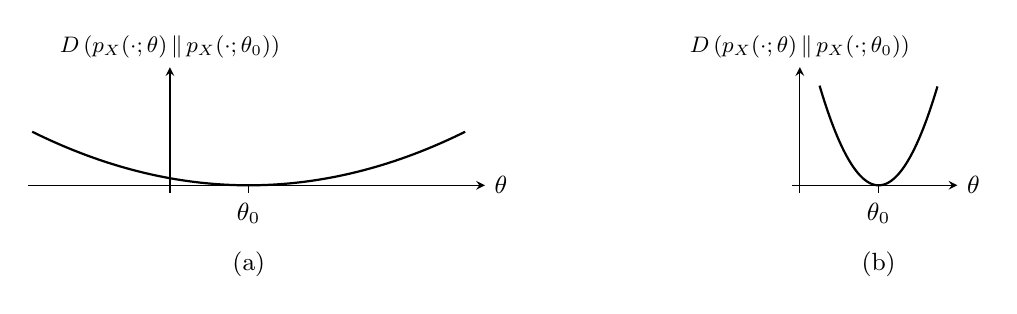
\begin{tikzpicture}
\shorthandoff{>}
%
\pgfmathsetmacro{\t}{1}
\pgfmathsetmacro{\dx}{8}
%
% peque�a curvatura
\draw[>=stealth,->] (-1.8,0)--(4,0) node[right]{\small $\theta$};
\draw[>=stealth,->] (0,-.1)--(0,1.5) node[above,scale=.9]
{\small $D\left( p_X(\cdot;\theta) \, \| \, p_X(\cdot;\theta_0) \right)$};
\draw[thick,domain=-1.75:3.75,samples=200] plot (\x,{.09*abs(\x-\t)^2});
\draw (\t,0)--(\t,-.1) node[below]{\small $\theta_0$};
%
% granda curvatura
\draw[>=stealth,->] ({-.1+\dx},0)--({2+\dx},0) node[right]{\small $\theta$};
\draw[>=stealth,->] (\dx,-.1)--(\dx,1.5) node[above,scale=.9]
{\small $D\left( p_X(\cdot;\theta) \, \| \, p_X(\cdot;\theta_0) \right)$};
\draw[thick,domain=.25:1.75,samples=200] plot ({\x+\dx},{2.25*abs(\x-\t)^2});
\draw ({\t+\dx},0)--({\t+\dx},-.1) node[below]{\small $\theta_0$};
%
\draw (\t,-1) node{\small (a)};
\draw ({\t+\dx},-1) node{\small (b)};
\end{tikzpicture} \end{center}
%
\leyenda{Caso escalar \ $\Theta \subseteq \Rset$ \ (para la representaci\'on) de
  $\Dkl{}$  \ en  funci\'on de  \ $\theta$.   (a) Caso  con  \ $J_{\theta_0}(X)$
  ``peque\~no'' \  y (b) caso con  \ $J_{\theta_0}(X)$ \ ``grande''.  En el caso
  (b),  la determinaci\'on de  \ $\theta$  \ usando  $\Dkl{}$ \  va a  ser m\'as
  ``sencillo'' porque el m\'inimo es m\'as ``picado''.}
%
\label{fig:SZ:JCurvatura}
\end{figure}

\

Un otro  v\'inculo entre el  mundo de la  informaci\'on y el de  la estimaci\'on
aparece a trav\'es de la identidad  de de Bruijn~\footnote{A pesar de que tom\'o
  este nombre, esta identidad en su primera versi\'on fue publicada por Stam. En
  su papel~\cite{Sta59}, menciona que  esta identidad fue comunicada al Profesor
  van  Soest por el  Profesor de  Bruijn.}~\cite{Sta59, CovTho06,  Joh04, Bar84,
  Bar86, PalVer06}.  Esta identidad  caracteriza lo que  es conocido  como canal
gaussiano de la figura Fig~\ref{fig:SZ:deBruijnVerdu}-(a), \ie la salida \ $Y$ \
es una versi\'on ruidosa de la entrada.  La identidad vincula las variaciones de
entrop\'ia  de salida  con respeto  al  nivel de  ruido, y  la informaci\'on  de
Fisher.

\begin{teorema}[Identidad de de Bruijn]
  Sea \ $X$ \  un vector aleatorio continuo sobre un abierto  de \ $\Rset^d$ \ y
  admitiendo una matriz de covarianza, y sea \  $Y = X + T \Gauss$ \ donde \ $T$
  \ es determinista, $d  \times d'$ \ con \ $ d \le d'$,  de rango m\'aximo, y \
  $\Gauss$ \  un vector  gaussiano centrado y  de covarianza  \ $\Sigma_\Gauss$,
  independiente  de \  $X$ \  (ver  figura Fig.~\ref{fig:SZ:deBruijnVerdu}-(a)).
  Entonces, la  entrop\'ia de Shannon  y la informaci\'on  de Fisher de \  $Y$ \
  satisfacen
  %
  \[
  \nabla_T H(Y) = J(Y) \, T \, \Sigma_\Gauss
  \]
  %
  donde \ $\nabla_T \, \cdot$ \ es la matriz de componentes \ $\frac{\partial \,
    \cdot}{\partial T_{i,j}}$.  Si \ $T = T(\theta)$ \ depende de un par\'ametro
  escalar~\footnote{Si el  par\'ametro es  multivariado, hace falta  entender la
    desigualdad a trav\'es de derivas parciales con respeto a los componentes de
    $\theta$.}  $\theta$,
  %
  \[
  \frac{\partial}{\partial \theta}  H(Y) = \Tr\left( J(Y) \,  T \, \Sigma_\Gauss
    \, \frac{\partial T^t}{\partial \theta} \right)
  \]
\end{teorema}
%
\begin{proof}
  La clave de este resultado viene del hecho  de que la densidad \ $p$ \ de \ $T
  \Gauss$ \ satisface una  ecuaci\'on diferencial particular.  La distribuci\'on
  de  \ $T  \Gauss$  \ se  escribe \  $p(x)  = (2  \pi)^{-\frac{d}{2}} \left|  T
    \Sigma_\Gauss  T^t  \right|^{-\frac12} \exp\left(  -  \frac12  x^t \left(  T
      \Sigma_\Gauss T^t \right)^{-1} x \right)$ \  (el rango m\'aximo de \ $T$ \
  asegura  que \  $T  \Sigma_\Gauss T^t$  \  sea invertible).   Para una  matriz
  invertible $R$,  desarollando \ $|R|$  \ con respecto  a su l\'inea \  $i$, se
  obtiene que  \ $\frac{\partial |R|}{\partial R_{i,j}} =  R_{i,j}^*$ \ cofactor
  de \ $R_{i,j}$, dando por la regla de Cram\'er \ $\nabla_R |R| = |R| \, \left(
    R^{-1} \right)^t$ \ (ver tambi\'en~\cite[cap.~1~\&~9]{MagNeu99}), es decir \
  $\nabla_R |R|^{-\frac12}  = -\frac12 |R|^{-\frac12}  \left( R^{-1} \right)^t$.
  De    $\frac{\partial   |R|^{-\frac12}}{\partial    T_{i,j}}    =   \sum_{k,l}
  \frac{\partial      |R|^{-\frac12}}{\partial      R_{k,l}}      \frac{\partial
    R_{k,l}}{\partial  T_{i,j}}  =  -\frac12  |R|^{-\frac12}  \sum_{k,l}  \left(
    R^{-1} \right)_{l,k} \frac{\partial R_{k,l}}{\partial T_{i,j}}$ \ con \ $R =
  T  \Sigma_\Gauss  T^t$  \  (sim\'etrica)  y c\'alculos  b\'asicos  se  obtiene
  finalmente
  %
  \[
  \nabla_T  \left|   T  \Sigma_\Gauss  T^t  \right|^{-\frac12}  =   -  \left|  T
    \Sigma_\Gauss T^t \right|^{-\frac12} \left( T \Sigma_\Gauss T^t \right)^{-1}
  T \Sigma_\Gauss
  \]
  %
  Adem\'as, de \ $\left( T  \Sigma_\Gauss T^t \right) \left( T \Sigma_\Gauss T^t
  \right)^{-1}  =  I$ \  viene  \  $\frac{\partial  \left( T  \Sigma_\Gauss  T^t
    \right)^{-1}}{\partial T_{i,j}} = -  \left( T \Sigma_\Gauss T^t \right)^{-1}
  \frac{\partial \left( T \Sigma_\Gauss  T^t \right)}{\partial T_{i,j}} \left( T
    \Sigma_\Gauss T^t \right)^{-1}$ \  donde \ $e_i$ \ es el vector  con 1 en su
  componente \ $i$ \ y cero si no, dando
  %
  \begin{eqnarray*}
  \frac{\partial \left( x^t \left( T \Sigma_\Gauss T^t \right)^{-1} x
  \right)}{\partial T_{i,j}} & = & - x^t \left( T \Sigma_\Gauss T^t \right)^{-1}
  \left( e_i e_j^t \Sigma_\Gauss T^t + T \Sigma_\Gauss e_j e_i^t \right) \left( T
  \Sigma_\Gauss T^t \right)^{-1} x\\[2.5mm]
  %
  & = & - 2 \, e_i^t \left( T \Sigma_\Gauss T^t \right)^{-1} x x^t \left( T
  \Sigma_\Gauss T^t \right)^{-1} T \Sigma_\Gauss e_j
  \end{eqnarray*}
  %
  usando \ $x^t A e_k e_l^t B x = e_l^t B x x^t A e_k = e_k^t A^t x x^t B^t e_l$
  \  (escalares comutan y  un escalar  es igual  a su  transpuesta) y  usando la
  simetr\'ia de \ $T \Sigma_\Gauss T^t$.  Eso significa que
  %
  \[
  \nabla_T \left( x^t \left( T \Sigma_\Gauss T^t \right)^{-1} x \right) = - 2 \,
  \left(  T \Sigma_\Gauss  T^t \right)^{-1}  x  x^t \left(  T \Sigma_\Gauss  T^t
  \right)^{-1} T \Sigma_\Gauss,
  \]
  %
  dando
  %
  \[
  \nabla_T p(x)  = \left( - \left(  T \Sigma_\Gauss T^t \right)^{-1}  + \left( T
      \Sigma_\Gauss  T^t   \right)^{-1}  x   x^t  \left(  T   \Sigma_\Gauss  T^t
    \right)^{-1} \right) T \Sigma_\Gauss \, p(x)
  \]
  %
  Tomando la Hessiana de \ $p$ \  con respeto a \ $x$ \ se obtiene sencillamente
  que \ $p$ \ satisface la ecuaci\'on diferencial
  %
  \[
  \nabla_T p = \Hess_x p \, T \, \Sigma_\Gauss
  \]
  %
  Suponiende que  se puede intervertir derivadas  y integrales (ver~\cite{Bar84,
    Bar86}  donde  se  dan   condiciones  rigorosas),  $\displaystyle  p_Y(y)  =
  \int_{\Rset^d}  p_X(x)  p(y-x) \,  dx$  \  satisface  tambi\'en la  ecuaci\'on
  diferencial, y adem\'as
  %
  \begin{eqnarray*}
  \nabla_T H(Y) & = & - \int_{\Rset^d} \nabla_T \, p_Y(y) \log p_Y(y)
  \, dy - \int_{\Rset^d} \nabla_T \, p_Y(y) \, dy\\[2.5mm]
  %
  & = & - \left( \int_{\Rset^d} \Hess_y \, p_Y(y) \log p_Y(y) \, dy \right) T \,
  \Sigma_\Gauss - \nabla_T \int_{\Rset^d} p_Y(y) \, dy\\[2.5mm]
  %
  & = & - \left( \int_{\Rset^d} \left( \Hess_y \Big( p_Y(y) \log p_Y(y) \Big) -
  \Hess_y \, p_Y(y) - \frac{\nabla_y \, p_Y(y) \, \nabla_y \, p_Y(y)^t}{p_Y(y)}
  \right) \, dy \right) T \, \Sigma_\Gauss\\[2.5mm]
  %
  & = & - \left( \int_{\Rset^d} \Hess_y \Big( p_Y(y) \log p_Y(y) \Big) \, dy -
  \int_{\Rset^d} \Hess_y p_Y(y) \, dy \right) T \, \Sigma_\Gauss \: + \: J(Y) \, T
  \, \Sigma_\Gauss
  \end{eqnarray*}
  %
  usando la  ecuaci\'on diferencial  en la  segunda l\'inea, el  hecho de  que \
  $p_Y$ \ suma a  1 en la tercera l\'inea (su gradiente  es cero entonces), y la
  definici\'on de la matriz de Fisher  en la \'ultima l\'inea. Usando el teorema
  de la  divergencia (intergraci\'on por partes) aplicada  respectivamente a los
  componentes de \ $\nabla_y p_Y \log  p_Y$ \ y \ $\nabla_y p_Y$, suponiendo que
  estos gradientes se cancelan en el borde del dominio de integraci\'on, los dos
  t\'erminos integrales  valen cero, lo que  cierra la prueba  de la desigualdad
  general.  Adem\'as,  si \ $T =  T(\theta)$, la segunda desigualdad  sigue de \
  $\frac{\partial   \cdot}{\partial    \theta}   =   \sum_{i,j}   \frac{\partial
    \cdot}{\partial   T_{i,j}}   \frac{\partial   T_{i,j}}{\partial  \theta}   =
  \Tr\left( \nabla_T \, \frac{\partial T^t}{\partial \theta} \right)$.
\end{proof}

La versi\'on  inicial de la identidad de  de Bruijn, con \  $\Sigma_\Gauss = I$,
que se escribe
%
\[
\frac{d}{d\theta}     H(X+\sqrt{\theta}    \Gauss)    =     \frac12    \Tr\left(
  J(X+\sqrt{\theta} \Gauss) \right)
\]
%
se recupera  en el caso particular  \ $T =  \sqrt{\theta} I$.  En este  caso, la
ecuac\'ion diferencial satisfecha por la densidad  de probabilidad \ $p$ \ es la
{\it  ecuaci\'on del  calor}.  Esta  desigualdad cuantifica  las  variaciones de
entrop\'ias   bajo  variaciones   de  ``niveles''   del  ruido   del   canal  de
comunicaci\'on. De una  forma, caracteriza la robustez del  canal con respeto al
nivel de ruido gaussiano (la gaussiana juega de nuevo un rol central ac\'a).

\

Existe una  otra forma  muy similar  de esta desigualdad  debido a  Guo, Shamai,
Verd\'u, Palomar~\cite{GuoSha05,  PalVer06}. Esta versi\'on  vincula a\'un m\'as
el  mundo  de  la informaci\'on  y  el  de  la  estimaci\'on.   Del lado  de  la
comunicaci\'on, consiste a caracterizar  la informaci\'on mutua entre la entrada
\ $X$ \ de  un canal ruidoso y su salida, \  $Y = S X + \Gauss$ \  donde \ $S$ \
coresponde  a un  pre-tratamiento antes  de la  salida. Eso  es ilustrado  en la
figura  Fig.~\ref{fig:SZ:deBruijnVerdu}-(b).  Del lado  de la  estimaci\'on, uno
puede querer  estimar \ $X$  \ observando solamente  \ $Y$.  Es conocido  que el
estimador  que minimiza  el error  cuadr\'atico promedio  \  $\Esp\left[ \left\|
    \widehat{X}(Y)  - X  \right\|^2 \right]$  \  es la  esperanza condicional  \
$\widehat{X}(Y) = \Esp[X|Y]$.  \ Una caracter\'istica de un  estimador siendo su
matriz de covarianza,  se notar\'a \ $\E(X|Y) = \Esp\left[  \left( X - \Esp[X|Y]
  \right)   \left(   X  -   \Esp[X|Y]   \right)^2   \right]$   \  esta   matriz.
Sorpredentemente,  existe  tambi\'en  una  identidad  entre \  $I(X;Y)$  \  y  \
$\E(X|Y)$:
%
\begin{teorema}[Identidad de Guo--Shamai--Verd\'u]
  Sea \ $X$ \ un vector aleatorio  continuo sobre un abierto de \ $\Rset^{d'}$ \
  y admitiendo una  matriz de covarianza, y sea \  $Y = S X +  \Gauss$ \ donde \
  $S$  es determinista,  $d  \times d'$,  y  \ $\Gauss$  \  un vector  gaussiano
  centrado  y de covarianza  $\Sigma_\Gauss$, independiente  de $X$  (ver figura
  Fig.~\ref{fig:SZ:deBruijnVerdu}-(b)). Entonces, la informaci\'on mutua entre \
  $X$ \ e \ $Y$ \ y  la matriz de covarianza del estimador de error cuadr\'atico
  m\'inimo satisfacen
  %
  \[
  \nabla_S I(X;Y) = \Sigma_\Gauss^{-1} S \, \E(X|Y)
  \]
  %
  Si \ $S = S(\\sigma)$ \ depende de un par\'ametro escalar $\sigma$,
  %
  \[
  \frac{\partial}{\partial \sigma} I(X;Y) = \Tr\left( \Sigma_\Gauss^{-1} \, S \,
    \E(X|Y) \, \frac{\partial S^t}{\partial \sigma} \right)
  \]
\end{teorema}
%
\begin{proof}
  Notando  que \ $p_{Y|X}  (y,x) =  (2 \pi)^{-\frac{d}{2}}  \left| \Sigma_\Gauss
  \right|^{-\frac12}  \exp\left( -\frac12  (y-S  x)^t \Sigma_\Gauss^{-1}  (y-Sx)
  \right)$ \ viene \ $\nabla_S p_{Y|X}(x,y) = p_{Y|X}(x,y) \, \Sigma_\Gauss^{-1}
  (y - S  x) x^t$ \ (ver unos pasos  de la prueba de la  identidad de de Bruijn)
  as\'i que \ $\nabla_y p_{Y|X}(y,x) = p_{Y|X}(y,x) \, \Sigma_\Gauss^{-1} (y - S
  x)$, dando
  %
  \[
  \nabla_S  p_{Y|X}(y,x)  = \nabla_y  p_{Y|X}(y,x)  x^t  \qquad \mbox{y}  \qquad
  \nabla_S p_{X,Y}(x,y) = \nabla_y p_{X,Y}(x,y) x^t
  \]
  %
  (multiplicando ambos lados por $p_X$). Ahora, \ $I(X;Y) = H(Y) - H(Y|X) = H(Y)
  - H(\Gauss)$ \ (de la independencia, cuando \ $X  = x$, \ $Y = S x + \Gauss$ \
  gaussiana de misma convarianza que \ $\Gauss$  \ y de promedio \ $S x$), as\'i
  que
  %
  \begin{eqnarray*}
  \nabla_S I(X;Y) & = & \nabla_S H(Y)\\[2.5mm]
  %
  & = & - \int_{\Rset^d \times \Rset^{d'}} \nabla_S \Big( p_{X,Y}(x,y) \, \log
  p_Y(y) \Big) \, dx \, dy\\[2.5mm]
  %
  & = & - \int_{\Rset^d \times \Rset^{d'}} \nabla_S \, p_{X,Y}(x,y) \, \log p_Y(y) \,
  dx \, dy - \int_{\Rset \times \Rset} p_{X|Y}(x,y) \, \nabla_S \, p_Y(y) \, dx \,
  dy\\[2.5mm]
  %
  & = & \int_{\Rset^d \times \Rset^{d'}} \nabla_y p_{X,Y}(x,y) \, x^t \log p_Y(y)
  \, dx \, dy - \int_{\Rset^d} \nabla_S p_Y(y) \, dy\\[2.5mm]
  %
  & = & - \int_{\Rset^d \times \Rset^{d'}} \nabla_y p_Y(y) x^t p_{X|Y}(x,y) \, dx
  \, dy\\[2.5mm]
  %
  & = & - \int_{\Rset^d} \nabla_y p_Y(y) \, \Esp\left[X^t | Y = y \right] \, dy
  \end{eqnarray*}
  %
  La  segunda l\'inea  viene  de la  escritura  de \  $H(Y)$  usando $p_Y$  como
  marginale de $p_{X,Y}$ en $x$ y intercambiando gradiente e integral (ver pasos
  de la  prueba de la  desigualdad de de  Bruijn); la tercera de  $p_{X,Y}/p_Y =
  p_{X|Y}$;  en  la cuarta  se  usa  la  ecuaci\'on diferencial  satisfecha  por
  $p_{X,Y}$ en la  primera integral y integrando en $x$  en la segunda integral;
  la  quinta   l\'inea  se   obtiene  usando  el   teorema  de   la  divergencia
  (intergraci\'on por partes) en la integraci\'on en $y$ de la primera integral,
  e intercambiando  gradiente e integral  el la segunda  ($p_Y$ sumando a  1, el
  t\'ermino se cancela). Adem\'as,
  %
  \begin{eqnarray*}
  \nabla_y p_Y(y) & = & \int_{\Rset^{d'}} \nabla_Y p_{Y|X}(y,x) \, p_X(x) \,
  dx\\[2.5mm]
  %
  & = & - \Sigma_\Gauss^{-1} \int_{\Rset^{d'}} (y - S x) \, p_{Y|X}(y,x) \, p_X(x) \,
  dx\\[2.5mm]
  %
  & = & - \Sigma_\Gauss^{-1} \left( y - S \int_{\Rset^{d'}} x \, p_{X|Y}(x,y) \,dx
  \right) p_Y(y)\\[2.5mm]
  %
  & = & - \Sigma_\Gauss^{-1} \Big( y - S \Esp\left[X | Y=y \right] \Big) \, p_Y(y)
  \end{eqnarray*}
  %
  escribiendo $p_{Y|X}(y,x)  \, p_X(x) =  p_{X|Y}(x,y) \, p_Y(y)$ en  la tercera
  l\'inea. Esta ecuaci\'on permite escribir
  %
  \begin{eqnarray*}
  \nabla_S I(X;Y) & = & \Sigma_\Gauss^{-1} \int_{\Rset^d} \Big( y - S \Esp\left[X |
  Y=y \right] \Big) \Esp\left[X^t | Y=y \right] \, p_Y(y) \, dy\\[2.5mm]
  %
  & = & \Sigma_\Gauss^{-1} \left( \Esp\left[ Y \Esp\left[ X^t|Y \right] \right] - S
  \Esp\left[ \Esp\left[X | Y \right] \Esp\left[X | Y \right]^t \right]
  \right)\\[2.5mm]
  %
  & = & \Sigma_\Gauss^{-1} \left( \Esp\left[ Y X^t \right] - S \Esp\left[
  \Esp\left[X | Y \right] \Esp\left[X | Y \right]^t \right] \right)\\[2.5mm]
  %
  & = & \Sigma_\Gauss^{-1} S \left( \Esp\left[ X X^t \right] - \Esp\left[
  \Esp\left[X | Y \right] \Esp\left[X | Y \right]^t \right] \right)
  \end{eqnarray*}
  %
  la \'ultima l\'inea viniendo de $Y  = S X + \Gauss$ con $\Gauss$ independiente
  de  $X$ y  de  promedio 0.   La prueba  se  cierra notando  que \  $\Esp\left[
    \Esp[X|Y]  \right] = \Esp[X]$  \ y  por la  formula de  K\"onig-Huyggens. La
  segunda  identidad  viene  de  \  $\frac{\partial  \cdot}{\partial  \sigma}  =
  \Tr\left(  \nabla_S \,  \frac{\partial S^t}{\partial  \sigma} \right)$  \ (ver
  prueba de la identidad de de Bruijn).
\end{proof}
%
\noindent  La  primera versi\'on  de  esta  identidad se  recupera  con  \ $S  =
\sqrt{s}$, \ $\Sigma_\Gauss =  I$ \ y \ $X$ \ de  covarianza la identidad; $s$ \
es conocido como relaci\'on se\~nale/ruido en este caso.

Existen versiones a\'un m\'as completas  (con gradientes con respeto a la matriz
\  $\Sigma_\Gauss$  \  por  ejemplo)  que se  pueden  consultar  en~\cite{Joh04,
  PalVer06, PayPal09}.

\begin{figure}[h!]
%
\begin{center} 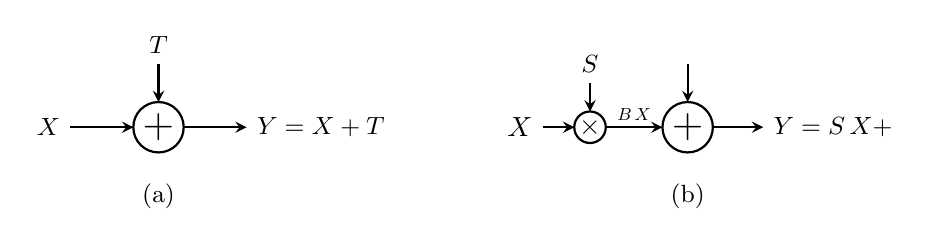
\begin{tikzpicture}[scale=.8]
\shorthandoff{>}
%
\begin{scope}
\draw[>=stealth,->,thick] (0,0) node[left]{\small $X$} --(1,0);
\draw[thick] (1.4,0) circle (.4);
\draw[>=stealth,->,thick] (1.4,1) node[above]{\small $T \N$} --(1.4,.4);
\node[align=center,scale=1.25] at (1.4,0){\large +};
\draw[>=stealth,->,thick] (1.8,0)--(2.8,0) node[right]{\small $Y = X + T \N$};
%
\end{scope}
%
\begin{scope}[xshift=7.5cm]
\draw[>=stealth,->,thick] (0,0) node[left]{$X$} --(.5,0);
\draw[thick] (.75,0) circle (.25);
\node[thick,align=center] at (.75,0){$\times$};
\draw[>=stealth,->,thick] (.75,.7) node[above]{\small $S$} --(.75,.25);
\draw[>=stealth,->,thick] (1,0)--(1.9,0);
\node[thick,align=center,scale=.7,above] at (1.45,0){\small $B \, X$};
\draw[thick] (2.3,0) circle (.4);
\draw[>=stealth,->,thick] (2.3,1) node[above]{\small $\N$} --(2.3,.4);
\node[align=center,scale=1.25] at (2.3,0){\large +};
\draw[>=stealth,->,thick] (2.7,0)--(3.5,0) node[right]{\small $Y = S \, X + \N$};
%
\end{scope}
\node at (1.4,-1.1){\small (a)};
\node at (9.8,-1.1){\small (b)};
\end{tikzpicture}
 \end{center}
%
\leyenda{Canal  de  comunicaci\'on  gaussiano  de  entrada  \  $X$.   (a)  Canal
  gaussiano usual, donde \ $T$ \ maneja los par\'ametros (nivel) del ruido.  (b)
  canal gaussiano con un preprocesamiento \ $S$ \ de la entrada.}
%
\label{fig:SZ:deBruijnVerdu}
\end{figure}
\

De la  desigualdad de  la potencia entr\'opica  y de  la identidad de  de Bruijn
surge  una otra  desigualdad implicando  la potencia  entr\'opica \  $N$ \  y la
informaci\'on de Fisher \ $J$.  Esta desigualdad es conocida como desigualdad de
Stam~\footnote{Como para  la identidad  de de Bruijn,  Stam mencion\'o  que esta
  desigualdad fue  comunicada al  Profesor van Soest  por el Profesor  de Bruijn
  quien  da una  prueba variacional  de la  desigualdad.}~\cite{CovTho06, Rio07,
  Sta59},     o    a    veces     ``desigualdad    isoperimetrica     para    la
entrop\'ia''~\cite{WanMad04}.
%
\begin{teorema}[Desigualdad de Stam]
  Sea  \  $X$   \  una  variable  aleatoria  continua   sobre  \  $\X  \subseteq
  \Rset^d$. Entonces,
  %
  \[
  N(X) \Tr\left( J(X) \right) \, \ge \, d
  \]
  %
  con igualdad si y solamente si \ $X$ \ es gaussiano de covarianza proporcional
  a la identidad.
\end{teorema}
%
\begin{proof}
  De la desigualdad de la potencia entr\'opica se obtiene \ $N(X + \sqrt{\theta}
  \Gauss)  \ge N(X)  + \theta  \left| \Sigma_\Gauss  \right|^{\frac1d}$. Tomando
  $\Sigma_\Gauss =  I$, se  obtiene \ $\forall  \, \theta  > 0,$ \  $\frac{N(X +
    \sqrt{\theta} \Gauss) - N(X)}{\theta}  \ge $.  Entonces, tomando el l\'imite
  \ $\theta \to 0$, aparece  que \ $\left. \frac{d}{d\theta} N(X + \sqrt{\theta}
    \Gauss)   \right|_{\theta  =   0}  \ge   1$.   La   prueba  se   cierra  con
  $\frac{d}{d\theta}  N(X   +  \sqrt{\theta}   \Gauss)  =  \frac{1}{2   \pi  \e}
  \frac{d}{d\theta}  \exp\left( \frac2d  H(X +  \sqrt{\theta} \Gauss)  \right) =
  \frac2d  N(X +  \sqrt{\theta}  \Gauss) \frac{d}{d\theta}  H(X +  \sqrt{\theta}
  \Gauss) = d N(X +  \sqrt{\theta} \Gauss) \Tr\left( J(X + \sqrt{\theta} \Gauss)
  \right)$ \ (por la identidad de  de Bruijn).  Adem\'as, la igualdad se obtiene
  cuando se  alcanza la cota  de la desigualdad  de la potencia  entr\'opica, es
  decir cuando \ $X$ \ es gaussiano de varianza proporcional a la del ruido, que
  es la identidad en este caso.
\end{proof}
%
Se  puede  ver  de  nuevo  el  rol  central  que  juega  la  gaussiana  en  esta
desigualdad. Adem\'as, de la desigualdad  de Stam se puede deducir tamb\'ien las
versiones escalares de  la desigualdad de Cram\'er-Rao. Viene  del hecho de que,
dada una matriz de covarianza, la entrop\'ia \ $H(X)$ \ es m\'axima cuando \ $X$
\ es gaussiano.  Entonces, para cualquier  \ $X$ \ de covarianza \ $\Sigma_X$, \
$N(X) \le \left| \Sigma_X \right|^{\frac1d}$,  dando de la desiguldad de Stam, \
$\left| \Sigma_X \right|^{\frac1d} \Tr\left( J(X)  \right) \ge d$ \ (y las otras
versiones  escalares de  la relaci\'on  determinente-traza).  Como  se  lo puede
esperar, se  obtiene la igualdad si y  solamente \ $X$ \  es gaussiano (potencia
entr\'opica alcanzando su  cota superior) y de matriz  la identidad (desiguladad
de Stam se saturando).

Varias   otras  pruebas   de  la   desigualdad  de   Stam  pueden   provenir  de
generalizaciones, por ejemplo debido a Lutwak o Bercher~\cite{Lut, Ber}.  \SZ{La
  secci\'on ZZZ lo va a rapidamente evocar. Ver caso discreto Kagan~\cite{Kag01}.}

\

\SZ{(1) Existe un data  proc ineq con Fisher, cf Rioul 07  ou Stam 59 ou Frieden
  04 o Kagan~\cite{KagYu08}; cf  aussi si $I_\theta(g(X)) \le  I_\theta(X)$ used in  Kagan-Smith 1999 ;
  (2) ver MinFisher Frieden p. 235, Berchet Vignat 2009, Ernst 2017; cf. travaux
  rederivant MQ de Frieden-Plastino-Soffer  (1999, 2002), Reginato 98, Bickel 81
}

% ========================= Ejemplos & Aplicaciones ========================== %

\seccion{Unos ejemplos y aplicaciones}
\label{Sec:SZ:Ejemplos}


% ================================= canal

\subseccion{Canal de transmisi\'on y su capacidad}
\label{Ssec:SZ:CanalCapacidad}

Siguiendo el  esquema de comunicaci\'on de  Shannon, un mensaje  que se modeliza
como  un vector  aleatorio~\footnote{De  punto  de vista  de  un receptor,  este
  mensaje es  desconocido. Adem\'as, se lo  puede ver como una  instancia de una
  clase  importante   de  posibles  mensajes,   justificando  la  modelizaci\'on
  aleatoria.} $X$  pasa por un  canal de comunicaci\'on  y se recibe  un mensaje
$Y$, vector  aleatorio. En el trabajo de  Shannon, el canal es  supuesto a ruido
aditivo,  es decir  que se  a\~nade un  ruido a  $X$.  De  manera  general, para
conocer la informaci\'on de $X$ que se recibe, se calcula la informaci\'on mutua
$I(X;Y)$, es  decir la cantidad de  informaci\'on que comparten la  entrada y la
salida  del  canal.  Lo  m\'as  $I$  es grande,  lo  m\'as  de informaci\'on  se
transmite.  Dado el canal, se puede arreglar $X$ (su distribuci\'on) de manera a
maximizar $I(X;Y)$,  es decir  la cantidad m\'axima  que se puede  transmitir en
este    canal.    Es    lo     que    es    conocido    como    capacidad    del
canal~\cite[part.~II~\&~III]{Sha48} (ver  tambi\'en~\cite{CovTho06, Rio07} entre
otros):
%
\begin{definicion}[Capacidad de canal]
\label{Def:SZ:CapacidadCanal}
%
  Sea un canal de transmisi\'on, $X$  su entrada e $Y$ su salida, como ilustrado
  figura  Fig.~\ref{Fig:SZ:CanalComunicacion}.  Sea  $p_X$ la  distribuci\'on de
  probabilidad de $X$. La capacidad $C$ del canal es definida por
  %
  \[
  C = \max_{p_X} \, I(X;Y).
  \]
\end{definicion}

\begin{figure}[h!]
%
\begin{center} 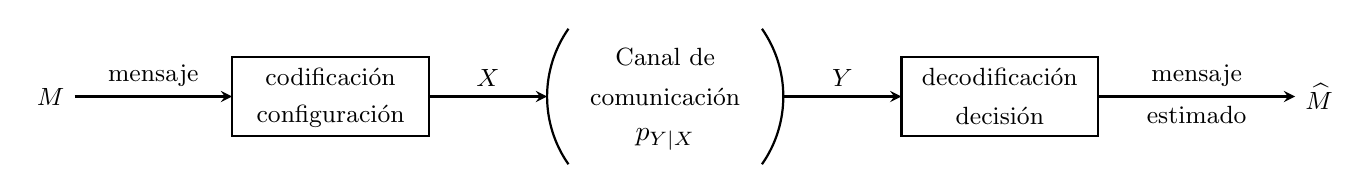
\begin{tikzpicture}
\shorthandoff{>}
%
% Mensaje
\draw[>=stealth,->,thick] (0,0) node[left]{\small $M$} --(2,0);
\draw (1,0) node[above]{\small mensaje};
%
% codificacion
\draw[thick] (2,-.5) rectangle (4.5,.5);
\draw (3.25,.25) node{\small codificaci\'on};
\draw (3.25,-.25) node{\small configuraci\'on};
%
% entrada del canal
\draw[>=stealth,->,thick] (4.5,0)--(6,0);
\draw (5.25,0) node[above]{\small $X$};
%
% Canal de com
\pgfmathsetmacro{\t}{35};
\pgfmathsetmacro{\r}{1.5};
\draw[thick] ({6+\r*(1+cos(180-\t))},{\r*sin(\t)}) arc (180-\t:180+\t:\r);
\draw[thick] ({6+\r*(1+cos(\t))},{-\r*sin(\t)}) arc (-\t:\t:\r);
\draw ({6+\r},.5) node{\small Canal de};
\draw ({6+\r},0) node{\small comunicaci\'on};
\draw ({6+\r},-.55) node{$p_{Y|X}$};
%
% salida
\draw[>=stealth,->,thick] ({6+2*\r},0)--({7.5+2*\r},0);
\draw ({6.75+2*\r},0) node[above]{\small $Y$};
%
% decodificacion/decision
\draw[thick] ({7.5+2*\r},-.5) rectangle ({10+2*\r},.5);
\draw ({8.75+2*\r},.25) node{\small decodificaci\'on};
\draw ({8.75+2*\r},-.25) node{\small decisi\'on};
%
% Mensaje estimado
\draw[>=stealth,->,thick] ({10+2*\r},0)--({12.5+2*\r},0) node[right]{\small $\widehat{M}$};
\draw ({11.25+2*\r},0) node[above]{\small mensaje};
\draw ({11.25+2*\r},0) node[below]{\small estimado};
\end{tikzpicture}
 \end{center}
%
\leyenda{Esquema de comunicaci\'on de Shannon.  En una primera etapa, un mensaje
  $M$ a  transmitir es  c\'odificado (ej.  c\'odigo  binario) o puesto  en forma
  (ej.  s\'imbolos  modulando una  funci\'on para que  sea anal\'ogica y  en una
  banda  de frecuencias  dada).  Sea  $X$ este  mensaje codificado  o  puesto en
  forma.  A la  recepci\'on, se mide $Y$ (ej.  versi\'on  ruidosa de $X$), antes
  de ser decodificado o usado para tomar una decisi\'on, $\widehat{M}$ siendo la
  estimaci\'on de  $M$ (ej.  s\'imbolos estimados  a partir de  $Y$).  Una etapa
  importante es el v\'inculo entre la entrada  $X$ y la salida $Y$ del canal, es
  decir la  cantidad de informaci\'on que  tienen en com\'un.   La capacidad del
  canal es la informaci\'on $I(X;Y)$ m\'axima con respeto a su entrada.}
\label{Fig:SZ:CanalComunicacion}
\end{figure}


% ================================= canal binario

\subsubseccion{Canal binario}
\label{Sssec:SZ:CanalBinario}

Suponiendo  que el  mensaje mandado  en un  canal es  una cadena  de s\'imbolos,
variables   aleatorias  independientes,   se  puede   concentrarse   sobre  cada
s\'imbolo. En este marco, un canal de comunicaci\'on lo m\'as simple es conocido
como  {\it canal  binario}~\cite[Sec.~15]{Sha48}: $X$  es una  variable definida
sobre $\X =  \{ 0 \, , \, 1  \}$; tal tipo de entrada es  natural, pensando a la
codificaci\'on  binaria.  La  salida $Y$  es tambi\'en  definida sobre  $\X$; se
puede imaginar medir y tomar una decisi\'on binaria usando la medida.  Tal canal
es  definido por  sus  probabilidaded de  transici\'on  $p_{Y|X=x}(y)$, \ie  las
probabilidades que un 0 (resp. un 1) se transmite correctamente o cambia en un 1
(resp. 0), \ie
%
\[
\varepsilon = P(Y  = 1 | X =  0) = 1 - P(Y  = 0 | X = 0)  \qquad \mbox{y} \qquad
\vartheta = P(Y = 0 | X = 1) = 1 - P(Y = 1 | X = 1).
\]
%
$\varepsilon$ y $\vartheta$ representan errores de comunicaci\'on.  Tal canal es
descrito      figura     Fig.~\ref{Fig:SZ:CanalBinario}-(a).       La     figura
Fig.~\ref{Fig:SZ:CanalBinario}-(b) da un esquema ``pr\'actico'' que podr\'ia ser
al origen  de un  tal canal.  Cuando  \ $\varepsilon  = \vartheta$, el  canal es
conocido como {\it canal binario sim\'etrico}.  Cuando \ $\varepsilon = 0$ \ y \
$\vartheta \in (0 \; 1)$, el canal es conocido como {\it canal binario en Z}.

\begin{figure}[h!]
\begin{center} 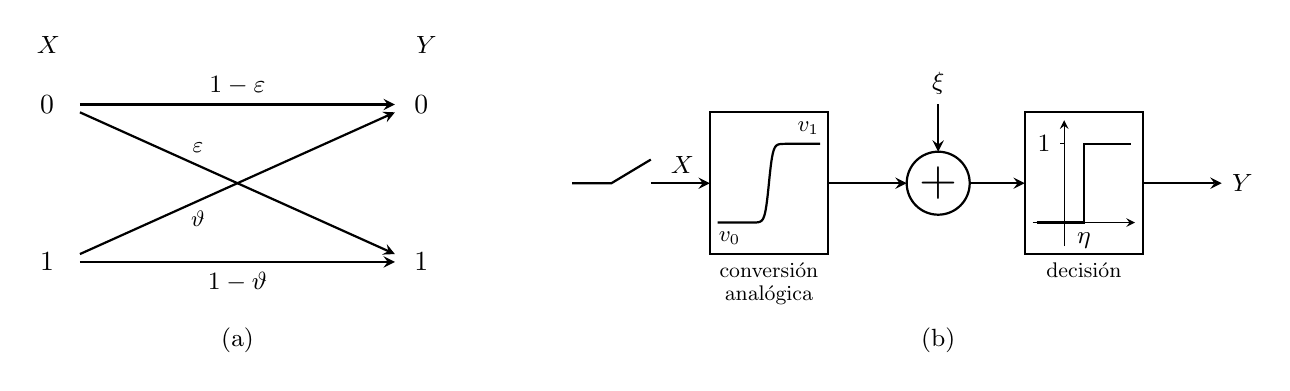
\begin{tikzpicture}
\shorthandoff{>}
%
\begin{scope}
\draw (-.4,1.75) node {\small $X$}; \draw (4.4,1.75) node {\small $Y$};
%
\draw[>=stealth,->,thick] (-.2,1) node[left]{0} (0,1) -- (4,1) node[right]{\ 0};
\draw (2,1) node[above]{\small $1-\varepsilon$};
%
\draw[>=stealth,->,thick] (-.2,-1) node[left]{1} (0,-1) -- (4,-1) node[right]{\ 1};
\draw (2,-1) node[below]{\small $1-\vartheta$};
%
\draw[>=stealth,->,thick] (0,.9)--(4,-.9);
\draw (1.5,.45) node[scale=.9]{\small $\varepsilon$};
%
\draw[>=stealth,->,thick] (0,-.9)--(4,.9);
\draw (1.5,-.45) node[scale=.9]{\small $\vartheta$};
%
\end{scope}
%
\begin{scope}[xshift=7cm]
%
% entrada
\draw[thick] (-.75,0)--(-.25,0)--(.25,.3);
\draw[>=stealth,->,thick] (.25,0)--(1,0);
%\draw[>=stealth,->,thick] (.25,-.5) node[below]{\small $X$} --(.25,.1);
\draw (.65,0) node[above]{\small $X$};
%
% puesta en niveles
\draw[thick] (1,-.9) rectangle (2.5,.9);
\draw (1.25,-.7) node[scale=.9]{\small $v_0$};
\draw (2.25,.7) node[scale=.9]{\small $v_1$};
\draw[thick,domain=-4.5:4.5,samples=100] (1.1,-.5) -- plot ({\x/10+1.75},{.5*tanh(2*\x)}) --(2.4,.5);
\draw (1.75,-.9) node[below,scale=.85]{\small conversi\'on};
\draw (1.75,-1.2) node[below,scale=.85]{\small anal\'ogica};
%
% adicion del ruido
\draw[>=stealth,->,thick] (2.5,0)--(3.5,0);
\draw[thick] (3.9,0) circle (.4);
\draw[>=stealth,->,thick] (3.9,1) node[above]{\small $\xi$} --(3.9,.4);
\draw (3.9,0) node[align=center,scale=1.5]{\large +};
%
% decision
\draw[>=stealth,->,thick] (4.3,0)--(5,0);
\draw[thick] (5,-.9) rectangle (6.5,.9);
\draw[>=stealth,->] (5.1,-.5)--(6.4,-.5);
\draw[>=stealth,->] (5.5,-.8)--(5.5,.8);
\draw[thick] (5.15,-.5)--(5.75,-.5)--(5.75,.5)--(6.35,.5);
\draw (5.75,-.5) node[below]{\small $\eta$};
\draw (5.5,.5)--(5.45,.5) node[left]{\small 1};
\draw (5.75,-.9) node[below,scale=.85]{\small decisi\'on};
%
% salida
\draw[>=stealth,->,thick] (6.5,0)--(7.5,0) node[right]{\small $Y$};
\end{scope}
\draw (2,-2) node {\small (a)};
\draw (10.9,-2) node {\small (b)};
\end{tikzpicture}
 \end{center}
%
\leyenda{(a): Canal binario.  La entrada $X$ definida  sobre $\X = \{ 0  \, , \,
  1\}$ pasa  por este canal  e $Y$  definida sobre $\Y  = \X$ es  recibido. Este
  canal es caracterizado por  las probabilidades de transici\'on $p_{Y|X=x}(y)$.
  (b): Esquema  que puede conducir al  canal binario; una variable  puede ser la
  salida de una puerta l\'ogica, con niveles $v_0$ (nivel bajo, codificando 0) y
  $v_1$  (nivel alto, codificando  1).  Se  puede imaginar  que este  voltaje es
  transmitido por un  canal a\~nandiendo un ruido $\xi$.   En la recepci\'on, se
  toma una  decisi\'on, por ejemplo  0 (resp.  1)  si la medida es  mayor (resp.
  menor)  que  $\eta  =   \frac{v_0  +  v_1}{2}+\Esp[\xi]$.   En  este  ejemplo,
  $\varepsilon$ \ y  \ $\vartheta$ \ van a  ser caracterizados completamente por
  la distribuci\'on  del ruido (y  de los dos  niveles posibles de  la entrada),
  pero no de la distribuci\'on $p_X$.}
\label{Fig:SZ:CanalBinario}
\end{figure}

En este caso, trabajando con bits, aparece leg\'itimo usar el logaritmo de base
2. Luego, sean
%
\[
r = P(X = 0),
\]
%
dando la distribuci\'on  de la entrada. La distribuci\'on de la  salida va a ser
dada a partir de $s = P(Y = 0) = P(Y = 0 | X = 0) P(X = 0) + P(Y = 0 | X
= 1) P(X = 1)$ es decir
%
\[
s = P(Y  = 0) = \vartheta +  r (1-\varepsilon-\vartheta).
\]
%
La informaci\'on  mutua se escribe  \ $I_2(X;Y) =  H_2(Y) - H_2(Y|X) =  H_2(Y) -
H_2(Y|X=0) P(X = 0) + H_2(Y|X=1) P(X = 1)$, lo que toma la expresi\'on
%
\[
I_2(X;Y) = h_2(s) - r h_2(\varepsilon) - (1-r) h_2(\vartheta),
\]
%
donde $h_2(u) = -  u \log_2 u - (1-u) \log_2 (1-u)$  es la entrop\'ia binaria en
bits.  Para calcular la capacidad $C_2$  en bits, hace falta maximizar $I_2$ con
respeto   a   $r$.    Diferenciando    $I_2$   en   $r$,   \ie   $\frac{\partial
  I_2(X;Y)}{\partial  r}  =  \frac{\partial h_2(s)}{\partial  s}  \frac{\partial
  s}{\partial r} - h_2(\varepsilon) + h_2(\vartheta)$, es decir
%
\[
\frac{\partial I_2(X;Y)}{\partial  r} = (1-\varepsilon-\vartheta)  \log_2 \left(
  \frac{1-s}{s} \right) - h_2(\varepsilon) + h_2(\vartheta).
\]
%
\begin{itemize}
\item Claramente,
  %
  \[
  \vartheta = 1-\varepsilon \quad \Rightarrow \quad C_2 = 0.
  \]
  %
  Viene del hecho  que para $\vartheta = 1-\varepsilon$,  de $h_2(\varepsilon) =
  h_2(1-\varepsilon)$ se deduce que $I_2(X;Y)  = 0$ constante. De hecho, en este
  caso, un 0 en la salida puede venir  de un 0 o 1 con probabilidades iguales, y
  lo mismo para  un 1 en la  salida; en otros t\'erminos, la  salida aparece ser
  independiente de la entrada.  Eso se verifica formalmente con $s = \vartheta$,
  dando $p_{Y|X=x}  = p_Y$, dando una  informaci\'on mutua nula,  y entonces una
  capacidad nula.
%
\item Si $\vartheta  \ne 1-\varepsilon$, la derivada de $I_2$  con respeto a $r$
  se anula para $s = s^\opt$ ($r = r^\opt$),
  %
  \[
  s^\opt = \frac{1}{1 +  2^{\frac{h(\varepsilon) - h(\vartheta)}{1 - \varepsilon
        -  \vartheta}}}  \qquad \mbox{siendo}  \qquad  r^\opt  = \frac{s^\opt  -
    \vartheta}{1 - \varepsilon - \vartheta},
  \]
  %
  y  dando   un  extremo   para  $I_2$.   A   continuaci\'on,  $\frac{\partial^2
    I_2}{\partial  r^2} = \frac{(1-\varepsilon-\vartheta)^2}{s  (1-s)} >  0$ (en
  particular para el $s$ ``\'optimo''),  probando que el extremo es un m\'aximo.
  Poniendo  la expresi\'on de  $r^\opt$ en  la formula  de $I_2(X;Y)$,  luego de
  muchos c\'alculos (b\'asicos), se obtiene
  %
  \[
  C_2  =  \log_2\left(  1  +  2^{\frac{h_2(\varepsilon)  -  h_2(\vartheta)}{1  -
        \varepsilon   -  \vartheta}}   \right)  -   \frac{(1  -   \vartheta)  \,
    h_2(\varepsilon)  -   \varepsilon  \,  h_2(\vartheta)}{1   -  \varepsilon  -
    \vartheta}.
  \]
  %
  Cuando  $\vartheta   \to  1-\varepsilon$,  notando   que  $h_2(\varepsilon)  =
  h_2(1-\varepsilon)$ y  tomando el  l\'imite de esta  formula, se  recupera que
  $C_2 \to 0$.
  %
  % ---
  %
  % \newline{\color{red}\bf �Interpretacion?  no hay combinacion convexa
  %   $\frac{\varepsilon}{1-\varepsilon-\vartheta}$ siendo del mismo signo que
  %   $\frac{1-\vartheta}{1-\varepsilon-\vartheta}$; nota: $C
  %   = \log_2\left( 1 + 2^{-
  %       \frac{h(1-\vartheta)-h(\varepsilon)}{(1-\vartheta)-\varepsilon}}
  %   \right) + \frac{1}{\varepsilon
  %     (1-\vartheta)} \frac{(1-\vartheta) h(1-\vartheta) - \varepsilon
  %     h(\varepsilon)}{\vartheta - (1-\varepsilon)}$}
\end{itemize}
%
\noindent De  \ $I_2(X;Y) = H_2(Y)  - H_2(Y|X) \le H_2(Y)  \le 1$ bit  \ ($Y$ es
binario, de entrop\'ia m\'axima en el caso uniforme), aparece sin c\'alculos que
%
\[
C_2 \le 1 \: \mbox{bit},
\]
%
\ie  la capacidad  es menor  que 1  bit: para  transmitir informaci\'on  en este
canal, hace falta introducir redundancia en  el mensaje.  Se alcanza \ $C_2 = 1$
bit si, (i) por  un lado $H_2(Y|X) = 0$, es decir  \ $r h_2(\varepsilon) + (1-r)
h_2(\vartheta) = 0$ \ y adem\'as (ii) \ $h_2(s) = 1$.  Estudiando cada caso (ej.
con \ $r = 0$ \ y \ $\vartheta =  0$ \ se satisface (i) pero no (ii) porque \ $s
= 0$), se obtiene que
%
\[
C_2  =  1  \qquad  \Leftrightarrow  \qquad  r =  \frac12  \quad  \mbox{y}  \quad
\varepsilon = \vartheta = \frac{1 \pm 1}{2}.
\]
%
Para  $\varepsilon =  \vartheta =  0$ el  canal es  perfecto, mientras  que para
$\varepsilon =  \vartheta =  1$ el  canal es llamado  {\it canal  volteando}; en
ambos casos, se recupera la entrada (o directamente, o tomando el opuesto) ``sin
perdida''.

La  figura  Fig.~\ref{Fig:SZ:ICanalBinario}  representa la  informaci\'on  mutua
$I(X;Y)$ para unos  canales ($\varepsilon$ y $\vartheta$ dados)  en funci\'on de
$r$.  Se nota que la curva es c\'oncava y tiene un m\'aximo \'unico~\footnote{De
  manera general, de la escritura de $I$ con entrop\'ias condicionales, para $X$
  definido sobre $\X$ e  $Y$ sobre $\Y$, da \ $0 \le C \le  \min( \log |\X| \, ,
  \, \log |\Y|  )$.  \ Adem\'as, $p_{Y|X=x}$  depende solo del canal y  no de la
  entrada, as\'i que  para \ $p_X =  \pi_1 p_{(1)} + \pi_2 p_{(2)}$  \ ($\pi_2 =
  1-\pi_1$) se obtiene \ $p_Y = \pi_1 q_{(1)} + \pi_2 q_{(2)}$ \ con \ $q_{(i)}$
  \ distribuci\'on de la salida corespondiente a una entrada de distribuci\'on \
  $p_{(i)}$.   Ahora, de  $I(X;Y) =  H(Y)-H(Y|X)$, el  segundo  t\'ermino siendo
  dependiente solamente del canal, de la concavidad de $H$ se obtiene de que $I$
  es c\'oncava con respeto a  $p_X$.  A continuaci\'on, $p_X$ parteneciendo a un
  convexo,  $I$ tiene un  m\'aximo que  es \'unico.},  capacidad del  canal.  La
figura  Fig.~\ref{Fig:SZ:CCanalBinario}  representa la  capacidad  del canal  en
funci\'on  de  \   $\varepsilon$  \  y  \  $\vartheta$   as\'i  que  unos  casos
particulares/cortes.

En  el caso  particular  $\varepsilon  = \vartheta$,  conocido  como {\it  canal
  sim\'etico}, la capacidad es
%
\[
C_2 = 1 - h_2(\varepsilon)
\]
%
(alcanzada  con  una entrada  uniforme).   Como visto  en  el  caso general,  la
capacidad vale 1  bit si y solamente si  \ $h_2(\varepsilon) = 0$, \  es decir \
$\varepsilon = 0$ \ o \ $\varepsilon = 1$.  Al rev\'es, la capacidad es m\'inima
cuando $H_2$ est m\'aximo, es decir  para \ $\varepsilon = \vartheta = \frac12$,
\ y  \ $C_2 = 0$  \ (instancia particular  de \ $\vartheta =  1-\varepsilon$). \
$h_2(\varepsilon)$  \  es la  perdida  en bit  para  cada  bit transmitido.   La
capacidad  \  $C_2$   \  en  funci\'on  de  \   $\varepsilon$\  es  dada  figura
Fig.~\ref{Fig:SZ:CCanalBinario}-(b).

En el  caso particular  $\varepsilon = 0$,  conocido como  {\it canal en  Z}, la
capacidad es
%
\[
C_2 = \log_2\left( 1 +  2^{- \frac{h_2(\vartheta)}{1-\vartheta}} \right).
\]
%
Se nota  en este caso tambi\'en  que la capacidad  alcanza 1, su m\'aximo,  si y
solamente  si \  $\vartheta  = 0$  \  (canal perfecto).   Al  rev\'es, cuando  \
$\vartheta  \to 1$,  \  $C \to  0$, \  instancia  particular de  \ $\vartheta  =
1-\varepsilon$.   La capacidad \  $C_2$ \  en funci\'on  de $\vartheta$  es dada
figura Fig.~\ref{Fig:SZ:CCanalBinario}-(c).

%{\bf\color{red} C parecido a la de Shannon caso continuo. Interpretacion?}

\begin{figure}[h!]
%
\begin{center} \begin{tikzpicture}[scale=2]
\shorthandoff{>}
%
%
% ----- Canal general
%
\begin{scope}
\pgfmathsetmacro{\p}{.4};% varepsilon
\pgfmathsetmacro{\q}{.01};% vartheta
%
\pgfmathsetmacro{\dpr}{1-\p-\q};
\pgfmathsetmacro{\hp}{-\p*log2(\p)-(1-\p)*log2(1-\p)};% h(varepsilon)
\pgfmathsetmacro{\hq}{-\q*log2(\q)-(1-\q)*log2(1-\q)};% h(vartheta)
\pgfmathsetmacro{\dh}{\hp-\hq};
%
\pgfmathsetmacro{\bopt}{1/(1+(2^((\hp-\hq)/\dpr)))};% s opt
\pgfmathsetmacro{\aopt}{(\bopt-\q)/\dpr};% r opt
\pgfmathsetmacro{\Capa}{-log2(\bopt)-((1-\q)*\hp-\p*\hq)/\dpr};
%
\draw[>=stealth,->] (-.2,0)--(1.2,0) node[right]{\small $r$};
\draw[>=stealth,->] (0,-.2)--(0,1.2) node[above]{\small $I_2(X;Y)$};
%
\draw[thick,domain=0:1,samples=100] (0,0)-- plot (\x,
{-(\q+\dpr*\x)*log2(\q+\dpr*\x)-(1-\q-\dpr*\x)*log2(1-\q-\dpr*\x)-\x*\hp-(1-\x)*\hq)})
--(1,0);
%
\draw (\aopt,0)--(\aopt,-.05) node[below]{\small $r^\opt$};
\draw (1,0)--(1,-.05) node[below]{\small 1};
\draw (0,\Capa)--(-.05,\Capa) node[left]{\small $C_2$};
\draw (0,1)--(-.05,1) node[left]{\small 1};
\end{scope}
%
%
% ----- Canal simetrico
%
\begin{scope}[xshift=2.5cm]
\pgfmathsetmacro{\p}{.05};
%
\pgfmathsetmacro{\dpr}{1-2*\p};
\pgfmathsetmacro{\hp}{-\p*log2(\p)-(1-\p)*log2(1-\p)};
%
\pgfmathsetmacro{\Capa}{1-\hp};
%
\draw[>=stealth,->] (-.2,0)--(1.2,0) node[right]{\small $r$};
\draw[>=stealth,->] (0,-.2)--(0,1.2) node[above]{\small $I_2(X;Y)$};
%
\draw[thick,domain=0:1,samples=100] (0,0)-- plot (\x,
{-(\p+\dpr*\x)*log2(\p+\dpr*\x)-(1-\p-\dpr*\x)*log2(1-\p-\dpr*\x)-\hp)})
--(1,0);
%
\draw (.5,0)--(.5,-.05) node[below]{\small $r^\opt$};
\draw (1,0)--(1,-.05) node[below]{\small 1};
\draw (0,\Capa)--(-.05,\Capa) node[left]{\small $C_2$};
\draw (0,1)--(-.05,1) node[left]{\small 1};
\end{scope}
%
%
% ----- Canal en Z
%
\begin{scope}[xshift=5cm]
\pgfmathsetmacro{\q}{.3};
%
\pgfmathsetmacro{\dpr}{1-\q};
\pgfmathsetmacro{\hq}{-\q*log2(\q)-(1-\q)*log2(1-\q)};
%
\pgfmathsetmacro{\bopt}{1/(1+(2^(-\hq/\dpr)))};
\pgfmathsetmacro{\aopt}{(\bopt-\q)/\dpr};
\pgfmathsetmacro{\Capa}{-log2(\bopt)};
%
\draw[>=stealth,->] (-.2,0)--(1.2,0) node[right]{\small $r$};
\draw[>=stealth,->] (0,-.2)--(0,1.2) node[above]{\small $I_2(X;Y)$};
%
\draw[thick,domain=0:1,samples=100] (0,0)-- plot (\x,
{-(\q+\dpr*\x)*log2(\q+\dpr*\x)-(1-\q-\dpr*\x)*log2(1-\q-\dpr*\x)-(1-\x)*\hq)})
-- (1,0);
%
\draw (\aopt,0)--(\aopt,-.05) node[below]{\small $r^\opt$};
\draw (1,0)--(1,-.05) node[below]{\small 1};
\draw (0,\Capa)--(-.05,\Capa) node[left]{\small $C_2$};
\draw (0,1)--(-.05,1) node[left]{\small 1};
\end{scope}
\node at  (.5,-.6){\small (a)};
\node at  (3,-.6){\small (b)};
\node at  (5.5,-.6){\small (c)};
\end{tikzpicture}
 \end{center}
%
\leyenda{Informaci\'on mutua  (en bits) entrada-salida \ $I_2(X;Y)$  \ del canal
  binario en funci\'on de \ $r = P(X  = 0)$.  \ (a): \ $\varepsilon = 0.4$ \ y
  \  $\vartheta = 0.01$;  \ (b):  \ $\varepsilon  = \vartheta  = 0.05$  \ (canal
  sim\'etico); \ (c): \  $\varepsilon = 0$ \ y \ $\vartheta  = 0.05$ \ (canal en
  Z).}
%
\label{Fig:SZ:ICanalBinario}
\end{figure}

\

\begin{figure}[h!]
%
\begin{center} \begin{tikzpicture}[scale=2]
\shorthandoff{>}
%
%
% ----- Canal general
%
\begin{scope}
% C(\varepsilon,\vartheta)
%\begin{axis}[colorbar,domain=.01:.99, domain y=.01:.99, samples=10,  samples y=10,
%view={0}{90},  colormap/blackwhite,
%xlabel={\small $\varepsilon$}, ylabel={\small $\vartheta$}, xscale=.27, yscale=.27]
%\addplot3[surf,patch to triangles,shader=interp]
%%{5*sin(deg(2*pi*x))*exp(-4*pi*pi*y)};
%{log2(1+2^((-\x*log2(\x)-(1-\x)*log2(1-\x)+\y*log2(\y)+(1-\y)*log2(1-\y))/(1-\x-\y)))
%+((1-\y)*(\x*log2(\x)+(1-\x)*log2(1-\x))-\x*(\y*log2(\y)+(1-\y)*log2(\y)))/(1-\x-\y)};
%\end{axis}
%\draw(0,0) node{\color{red}\bf A faire};
\draw(1,.75) node{
\includegraphics[width=4cm]{TIKZ_SZ/CapacidadBinaria}};
\draw[>=stealth,->] (-.1,0)--(1.7,0) node[below]{\small $\varepsilon$};
\draw[>=stealth,->] (0,-.1)--(0,1.7) node[left]{\small $\vartheta$};
\draw (1.5,0)--(1.5,-.05) node[below,scale=.8]{\small 1};
\draw (0,1.5)--(-.05,1.5) node[left,scale=.8]{\small 1};
%
\draw (2.075,.02) node[scale=.8]{\small 0};
\draw (2.075,1.48) node[scale=.8]{\small 1};
\end{scope}
%
%
% ----- Canal simetrico
%
\begin{scope}[xshift=3.2cm,scale=1.3]
%
\draw[>=stealth,->] (-.1,0)--(1.2,0) node[right]{\small $\varepsilon$};
\draw[>=stealth,->] (0,-.1)--(0,1.2) node[above]{\small $C_2$};
%
\draw[thick,domain=.01:.99,samples=100] (0,1)-- plot (\x,
{1+\x*log2(\x)+(1-\x)*log2(1-\x)})
--(1,1);
%
\draw (.5,.75) node[scale=.8]{\small $(\vartheta = \varepsilon)$};
\draw (1,0)--(1,-.05) node[below,scale=.8]{\small 1};
\draw (0,1)--(-.05,1) node[left,scale=.8]{\small 1};
\end{scope}
%
%
% ----- Canal en Z
%
\begin{scope}[xshift=6cm,scale=1.3]
%
\draw[>=stealth,->] (-.2,0)--(1.2,0) node[right]{\small $\vartheta$};
\draw[>=stealth,->] (0,-.2)--(0,1.2) node[above]{\small $C_2$};
%
\draw[thick,domain=.01:.99,samples=100] (0,1)-- plot (\x,
{log2(1+2^(log2(1-\x)+(\x/(1-\x))*log2(1-\x)))})
-- (1,0);
%
\draw (.75,.75) node[scale=.8]{\small $(\varepsilon = 0)$};
\draw (1,0)--(1,-.05) node[below,scale=.8]{\small 1};
\draw (0,1)--(-.05,1) node[left,scale=.8]{\small 1};
\end{scope}
\draw (.8,-.4) node {\small (a)};
\draw (3.85,-.4) node {\small (b)};
\draw (6.75,-.4) node {\small (c)};
\end{tikzpicture}
 \end{center}
%
\leyenda{Capacidad  \ $C_2$ \  del canal  binario. \  (a): \  en funci\'on  de \
  $\varepsilon$ \  y \ $\vartheta$. \ (b):  \ en funci\'on de  \ $\varepsilon$ \
  para el canal sim\'etico ($\varepsilon = \vartheta$); \ (c): \ en funci\'on de
  \ $\vartheta$ \ para \ $\varepsilon = 0$ \ (canal en Z).}
%
\label{Fig:SZ:CCanalBinario}
\end{figure}

En~\cite{CovTho06,  Rio07}  entre  otros,  se estudian  diversos  otros  canales
discretos, binarios  o con m\'as estados.   Unos son representados  en la figura
Fig.~\ref{Fig:SZ:CanalesDiscretos}     (ver     tambi\'en~\cite{Sha48,    Eli57}
o~\cite{Ari72} para el c\'alculo num\'erico de la capacidad en el caso general).


\begin{figure}[h!]
%
\begin{center} 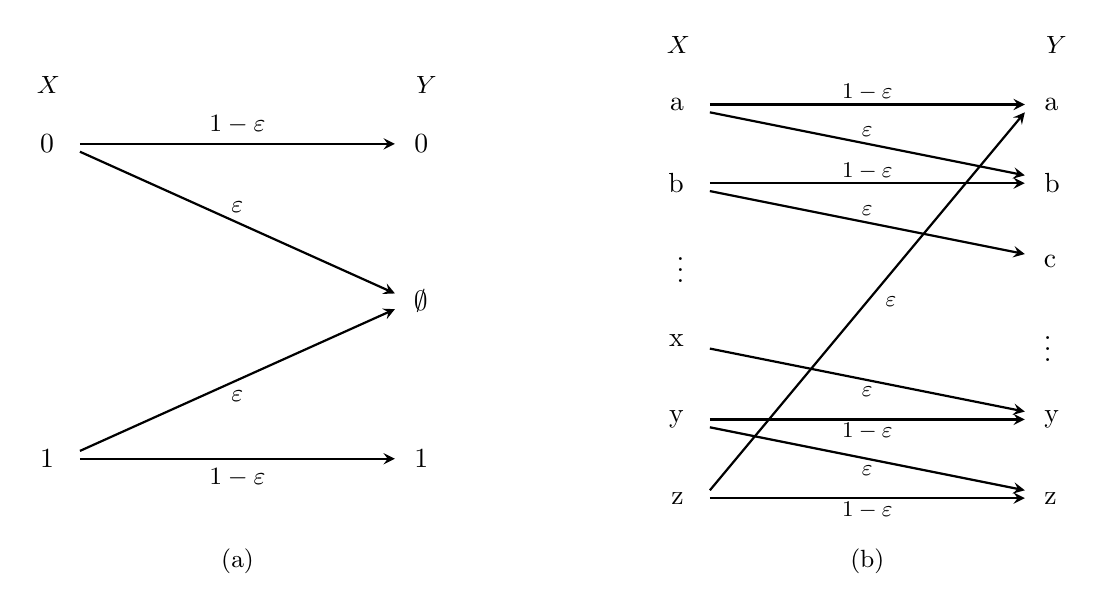
\begin{tikzpicture}
\shorthandoff{>}
%
% Canal borrador
\begin{scope}
\draw (-.4,2.75) node {\small $X$}; \draw (4.4,2.75) node {\small $Y$};
%
\draw[>=stealth,->,thick] (-.2,2) node[left]{0} (0,2) -- (4,2) node[right]{\ 0};
\draw (2,2) node[above]{\small $1-\varepsilon$};
%
\draw[>=stealth,->,thick] (-.2,-2) node[left]{1} (0,-2) -- (4,-2) node[right]{\ 1};
\draw (2,-2) node[below]{\small $1-\varepsilon$};
%
\draw[>=stealth,->,thick] (0,1.9)--(4,.1);
\draw (2,1.2) node{\small $\varepsilon$};
\draw[>=stealth,->,thick] (0,-1.9)--(4,-.1);
\draw (2,-1.2) node{\small $\varepsilon$};
\draw (4,0) node[right]{\ $\emptyset$};
%
\end{scope}
%
% Canal typewriter
\begin{scope}[xshift = 8cm]
\draw (-.4,3.25) node {\small $X$}; \draw (4.4,3.25) node {\small $Y$};
%
% lineas sin error
\draw[>=stealth,->,thick] (-.2,2.5) node[left]{a} (0,2.5) -- (4,2.5) node[right]{\ a};
\draw (2,2.65) node[scale=.9]{\small $1-\varepsilon$};
\draw[>=stealth,->,thick] (-.2,1.5) node[left]{b} (0,1.5) -- (4,1.5) node[right]{\ b};
\draw (2,1.65) node[scale=.9]{\small $1-\varepsilon$};
\draw (-.2,.5) node[left]{$\vdots$}; \draw (4,-.5) node[right]{\ $\vdots$};
\draw[>=stealth,->,thick] (-.2,-1.5) node[left]{y} (0,-1.5) -- (4,-1.5) node[right]{\ y};
\draw (2,-1.65) node[scale=.9]{\small $1-\varepsilon$};
\draw[>=stealth,->,thick] (-.2,-2.5) node[left]{z} (0,-2.5) -- (4,-2.5) node[right]{\ z};
\draw (2,-2.65) node[scale=.9]{\small $1-\varepsilon$};
%
% lineas con el error
\draw[>=stealth,->,thick] (0,2.4) -- (4,1.6);
\draw (2,2.15) node[scale=.9]{\small $\varepsilon$};
\draw[>=stealth,->,thick] (0,1.4) -- (4,.6); \draw (4,.5) node[right]{\ c};
\draw (2,1.15) node[scale=.9]{\small $\varepsilon$};
\draw[>=stealth,->,thick]  (-.2,-.5) node[left]{x} (0,-.6) -- (4,-1.4);
\draw (2,-1.15) node[scale=.9]{\small $\varepsilon$};
\draw[>=stealth,->,thick] (0,-1.6) -- (4,-2.4);
\draw (2,-2.15) node[scale=.9]{\small $\varepsilon$};
\draw[>=stealth,->,thick] (0,-2.4) -- (4,2.4);
\draw (2.3,0) node[scale=.9]{\small $\varepsilon$};
%
\end{scope}
\draw (2,-3.3) node{\small (a)};
\draw (10,-3.3) node{\small (b)};
\end{tikzpicture}
 \end{center}
%
\leyenda{Ejemplos de canales discretos usuales.  (a): canal borrador, donde un 0
  (de probabilidad de ocurrencia $r$) o 1 (de probabilidad de occurrencia $1-r$)
  puede  transmitirse correctamente or  ser borado/perdido  (estado $\emptyset$)
  con una  probabilidad $\varepsilon$.   Se calcula $I_2(X;Y)  = (1-\varepsilon)
  h_2(r)$, dando la capacidad $C_2  = 1-\varepsilon$, alcanzada para una entrada
  uniforme.   (b): canal tipo  machina de  escribir~\protect\footnotemark, donde
  cada letra  de un ensemble  de $n$  letras (ac\'a con  $n = 26$)  se transmite
  correctamente con una probabilidad $1-\varepsilon$  o a la letra siguiente (de
  manera c\'iclica) con una probabilidad $\varepsilon$.  De $I_n(X;Y) = H_n(Y) -
  H_n(Y|X) = H_n(Y)  - h_n(\varepsilon)$ se deduce que $I_n$  es m\'axima si $Y$
  es  uniforme,  lo que  es  posible  si  $X$ es  uniforma,  dando  $C_n =  1  -
  h_n(\varepsilon)$.}
\label{Fig:SZ:CanalesDiscretos}
\end{figure}
%
\footnotetext{Se mencionar\'a de  que en toda esta subsecci\'on,  no se necesita
  de que  $X$ y/o  $Y$ sean  variables aleatorias reales,  \ie pueden  tomar sus
  valores sobre cualquier espacio discreto (por ejemplo de letras).}


% ================================= canal gaussiano

\subseccion{Canal de transmisi\'on continuo gaussiano y su capacidad}
\label{Ssec:SZ:Canalgaussiano}

Un canal de  comunicaci\'on continuo relativamente simple es  conocido como {\it
  canal  gaussiano}~\cite[Sec.~25]{Sha48},~\cite{CovTho06,  Rio07}:  $X$ es  una
variable continua definida  sobre $\X \subseteq \Rset^d$ y la  salida $Y$ es una
versi\'on ruidosa de $X$, \ie $Y =  X + \xi$ con el ruido $\xi$ independiente de
$X$. En  el canal gaussiano, $\xi  \equiv \N$ es un  vector gaussiano.  Este
canal es tambi\'en definido por  su densidad de probabilidad ``de transici\'on''
$p_{Y|X=x}(y)$,  \ie por  la distribuci\'on  del ruido.   Tal canal  es descrito
figura  Fig.~\ref{Fig:SZ:CanalGaussiano}.   Se  supone  conocida  la  matriz  de
covarianza $\Sigma_\N$ del ruido, y se  nota $\Sigma_X$ la de la entrada. En
pr\'actica, no se puede mandar un mensaje a una potencia tan alta que se quiere,
lo que se traduce por una limitaci\'on
%
\[
\Tr\left(  \Sigma_X  \right) \le  \P,
\]
%
potencia l\'imite permitida por sampleo.

\begin{figure}[h!]
%
\begin{center} 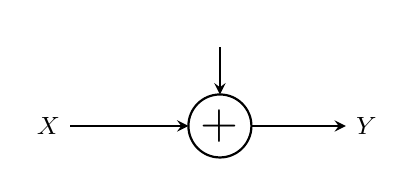
\begin{tikzpicture}
\shorthandoff{>}
%
%
% entrada
\draw[>=stealth,->,thick] (0,0) node[left]{\small $X$} --(1.5,0);
%
% adicion del ruido
\draw[thick] (1.9,0) circle (.4);
\draw[>=stealth,->,thick] (1.9,1) node[above]{\small $\N$} --(1.9,.4);
\draw (1.9,0) node[align=center,scale=1.5]{\large +};
%
% salida
\draw[>=stealth,->,thick] (2.3,0)--(3.5,0) node[right]{\small $Y$};
\end{tikzpicture}
 \end{center}
%
\leyenda{Canal gaussiano. La entrada $X$, modelizada por un vector aleatorio, es
  corrupta aditivamente por un ruido gaussiano $\N$ independiente de $X$. La
  salida es entonces $Y = X + \N$ y el canal es completamente descrito por \
  $p_{Y|X=x}(y)   =   p_\N(y-x)$  \   (obviamente   independiente  de   la
  distribuci\'on de la entrada).}
%
\label{Fig:SZ:CanalGaussiano}
\end{figure}


Por  definici\'on, la informaci\'on  mutua $I(X;Y)$  entrada-salida es  dada por
$I(X;Y) = H(Y) - H(Y|X) = H(Y) - H(\N)$. Maximizar $I(X;Y)$ es equivalente a
maximizar  $H(Y) =  H(X  + \N)$  sujeto  a $\Tr\left(  \Sigma_X \right)  \le
\P$. Fijando  un $\Sigma_X$, la  propiedad~\ref{Prop:SZ:cotamaximagaussiana} \ de
la entrop\'ia diferencial implica que $H(Y)$  sea m\'axima si y solamente si $Y$
es gaussiana,  es decir  si y solamente  si $X$  est gaussiana, dando  $I(X;Y) =
\frac12  \log \left|  \Sigma_X +  \Sigma_\N  \right| -  \frac12 \log  \left|
  \Sigma_\N \right|$. Tomando en cuenta  el l\'imite de potencia, hace falta
maximizar $\left| \Sigma_X  + \Sigma_\N \right|$ sujeto a  $\Tr \Sigma_X \le
\P$ \  y \ $\Sigma_X  \ge 0$ sim\'etica  lo que no  es trivial.  Se  encuentra el
enfoque  permitiendo solucionar  el problema  en~\cite[Sec.~9.4]{CovTho06}.  Sea
$U$, matriz  ortogonal ($U U^t =  U^t U = I$)  de los autovectores  de la matriz
$\Sigma_\N  \ge 0$  sim\'etica~\footnote{Se  recordar\'a de  que  $A \ge  0$
  significa que $A$  es definida no negativa.}, de  columnas $u_i$ ordenadas tal
que los autovalores corespondientes  $\lambda^\N_i$ sean en orden creciente,
\ie
%
\[
\Sigma_\N  =  U  \Diag\left(  \begin{bmatrix} \lambda^\N_1  &  \cdots  &
    \lambda^\N_d \end{bmatrix}^t \right) U^t  \qquad \mbox{con} \qquad 0 \le
\lambda^\N_1 \le \cdots \le \lambda^\N_d,
\]
%
donde $\Diag$ es la matriz diagonal teniendo los $\lambda_i$ en su diagonal (ver
notaciones).   Sea \ $R_X  = U^t  \Sigma_X U$.   Es sencillo  ver que  \ $\left|
  \Sigma_X + \Sigma_\N \right| = \left| R_X + \Lambda_\N \right|$ \ (de $|A B| =
|A| \,  |B|$) \ y  que \ $\Tr \Sigma_X  = \Tr R_X$  (de $\Tr(A B) =  \Tr(B A)$).
Entonces, el problema se reduce a  maximizar \ $\left| R_X + \Lambda_\N \right|$
\ sujeto a \  $\Tr R_X \le \P$ \ y \ $R_X \ge  0$ sim\'etica.  La desigualdad de
Hadamard ya evocada da \ $\left| R_X + \Lambda_\N \right| \le \prod_i \left( R_X
  +  \Lambda_\N  \right)_{i,i}  =  \prod_i  \left( \left(  R_X  \right)_{i,i}  +
  \lambda^\N_i   \right)$   \  donde   $(\cdot)_{i,i}$   denota  el   componente
$(i,i)$-\'esima  de la  matriz, con  igualdad si  y solamente  si \  $R_X$  \ es
diagonal: para maximizar \ $\left| R_X + \Lambda_\N \right|$, \ $R_X$ \ debe ser
entonces  diagonal (dada  una  diagonal, se  alcanza  el m\'aximo  si los  otros
t\'erminos son  nulos).  Es decir  que la base  que diagonaliza \  $\Sigma_\N$ \
debe  diagonalizar  tambi\'en $\Sigma_X$.   Sean  ahora  \  $\lambda^X_i$ \  los
t\'erminos  diagonales   de  $R_X$:  queda  que  maximizar   \  $\prod_i  \left(
  \lambda^X_i + \lambda^\N_i \right)$ \ sujeto a $\sum_i \lambda^X_i \le \P$ \ y
\ $\lambda^X_i \ge 0$.  Este problema de optimizaci\'on sujeto a una desigualdad
se  resuelva  con el  enfoque  de  Karush-Kuhn-Tucker~\footnote{Se introduce  el
  factor de Lagrange y se  maximiza \ $\prod_i \left( \lambda^X_i + \lambda^\N_i
  \right) +  \eta \sum_i \lambda^X_i$.  Eso  da \ $\lambda^X_i  + \lambda^\N_i =
  \lambda$ \  constante si $\lambda$ es  tal que se satisfaga  la positividad de
  $\lambda^X_i$, y $\lambda^X_i = 0$  sino.  En otras palabras, \ $\lambda^X_i =
  \left( \lambda -  \lambda^\N_i \right)_+$ con $\lambda$ el  factor de Lagrande
  despu\'es  de una  reescritura.  Queda  que maximizar  los  $\lambda^X_i$ para
  maximizar $\left| R_X + \Lambda_\N \right|$, es decir tomar $\lambda$ lo m\'as
  grande  que se  puede, pero  satisfaciendo  $\sum_i \lambda^X_i  \le \P$,  \ie
  alcanzando  la   igualdad.\label{Foot:SZ:KKT}}  (KKT)~\cite{Mil00,  CamMar09},
dando  \  $\lambda^X_i  = \left(  \lambda  -  \lambda^\N_i  \right)_+$ \  con  \
$(\cdot)_+ = \max(\cdot,0)$ \ y \ $\lambda$ \ tal que \ $\sum_i \left( \lambda -
  \lambda^\N_i \right)_+ = \P$.  En conclusi\'on, la capacidad es dada por
%
\begin{eqnarray*}
C =  \frac12 \log \left(  \frac{\left| \Sigma_\N +  \Sigma_X \right|}{\left|
      \Sigma_\N  \right|}  \right)  & \quad \mbox{con} \quad &  \Sigma_X  =  U
\Diag\left( \begin{bmatrix} \left(\lambda - \lambda^\N_1\right)_+ & \cdots & \left(\lambda -
    \lambda^\N_d \right)_+ \end{bmatrix}^t \right) U^t,\\[2.5mm]
%
& &  \lambda \ \mbox{ tal que } \:
\sum_i \left(\lambda - \lambda^\N_i \right)_+ = \P
\end{eqnarray*}
%
alcanzada por $X$ gaussiano de matriz de covarianza $\Sigma_X$ as\'i construida.

La  \'ultima condici\'on  se resuelva  a  trav\'es de  lo que  es conocido  como
``llenado   de   agua''   (water-filling   en   ingl\'es),   illustrado   figura
Fig.~\ref{Fig:SZ:WaterFilling}.   El  principio  es  parecido  a  tener  niveles
$\lambda^\N_i$  representando  las  potencias  del  ruido (en  la  base  que
diagonaliza la  matriz de covarianza), y  de ``llenar con agua''  hasta un nivel
$\lambda$ tal que el ``volumen''  a\~nadido vale $\P$; en cada $\lambda^\N_i$
se ha a\~nadido el $\lambda^X_i$~\cite[Sec.~9.4]{CovTho06}.

\begin{figure}[h!]
%
\begin{center} \begin{tikzpicture}
\shorthandoff{>}
%
% Filling
\filldraw[fill=gray!30] (3,2)--(3,1.5)--(2,1.5)--(2,1)--(1,1)--(1,.75)--(0,.75)--(0,2);
%
%Axes
\draw[>=stealth,->] (-.1,0)--(6,0);% node[right]{\small $i$};
\draw[>=stealth,->] (0,-.1)--(0,3);
\draw (0,.85) node[left]{\rotatebox{90}{\footnotesize Potencias}};
%
% neveles de ruido
\draw[thick] (0,.75)--(1,.75)--(1,0); \draw(.5,.375) node{\small $\lambda^\N_1$};
\draw[thick] (1,.75)--(1,1)--(2,1)--(2,0); \draw(1.5,.5) node{\small $\lambda^\N_2$};
\draw[thick] (2,1)--(2,1.5)--(3,1.5)--(3,0); \draw(2.5,.75) node{\small $\lambda^\N_3$};
\draw[thick] (3,1.5)--(3,2.25)--(4,2.25)--(4,0); \draw(3.5,1.125) node{\small $\lambda^\N_4$};
\draw[thick] (4,2.25)--(4,2.75)--(5,2.75)--(5,0); \draw(4.5,1.375) node{\small $\lambda^\N_5$};
\draw[thick] (5.5,1.25) node{\bf $\cdots$};
%
% nivel lambda y potencias de los X
\draw[thick] (0,2) node[left]{\small $\lambda$}--(3,2);
\draw (1,.75)--(1,2); \draw (.5,1.375) node{\small $\lambda^X_1$};
\draw (2,1)--(2,2); \draw (1.5,1.5) node{\small $\lambda^X_2$};
\draw (3,1.5)--(3,2); \draw (2.5,1.75) node{\small $\lambda^X_3$};
\end{tikzpicture}
 \end{center}
%
\leyenda{Principio   del  ``water-filling''   para  obtener   los  $\lambda^X_i$
  satisfaciendo  el v\'inculo de  potencia l\'imite  y permitiendo  de construir
  $\Sigma_X$ a partir  de la matriz diagonal de los $\lambda^X_i$  y la base que
  diagonaliza  la  covarianza  $\Sigma_\N$  del  ruido.  La  zona  en  grise
  representa esquem\'aticamente $\P$.}
%
\label{Fig:SZ:WaterFilling}
\end{figure}

En   el   caso   escalar,   se   obtiene
%
\[
C = \frac12 \log\left( 1 + \frac{\P}{\sigma_\N^2} \right),
\]
%
donde     $\frac{\P}{\sigma_\N^2}$     es     conocido    como     relaci\'on
se\~nale-ruido~\footnote{Esta formula es muy  parecida a la de Shannon, Laplume,
  o Clavier~\cite{Sha48,  Lap48, Cla48} (ver tambi\'en~\cite[Sec.~9.3]{CovTho06}
  o~\cite[Sec.~11.2]{Rio07}).   De hecho,  si se  considera  s\'imbolos mandados
  durante  $T$ segundos  cada  uno (s\'imbolos  puestos  en forma  para dar  una
  se\~nal anal\'ogica) usando una banda  de transmisi\'on $B$, por el teorema de
  Nyquist $B = \frac{1}{2 T}$ (caso l\'imite). Si el ruido es blanco en la banda
  $B$, de densidad espectral de potencia por unidad de frecuencia igual a $N_0$,
  para  un  s\'imbolo  la  relaci\'on  se\~nal-ruido  se  escribe  $\frac{\P}{N_0
    B}$. Adem\'as,  se calcula en general  la capacidad por unidad  de tiempo es
  decir la capacidad  por s\'imbolo divido por  $T = \frac{1}{2 B}$, \ie  $C = B
  \log\left( 1 +  \frac{\P}{N_0 B} \right)$ por segundos,  lo que es precisamente
  la capacidad calculdada por Shannon.  Esta es a veces conocida como formula de
  Shannon-Hartley.}

En~\cite{CovTho06,  Rio07}  por ejemplo,  se  dan  otros  ejemplos de  canal  de
comunicaci\'on   en   el   contexto   continuo   (entrada   $X_t$   siendo   una
se\~nal/proceso, canal filtrando, canal con retroacci\'on (o feedback), etc.).

% ================================= codificacion

\subseccion{Codificaci\'on entr\'opica sin perdida}
\label{Ssec:SZ:Codificacion}

El  problema  de  codificaci\'on  de  fuente  puede  presentarse  de  la  manera
siguiente~\cite[cap.~5]{CovTho06}  o   \cite[cap.~13]{Rio07}.   Sea  un  proceso
aleatorio $\left\{  X_t \right\}_{t \in \Zset}$,  supuesto estacionario, llamado
{\it  fuente}, donde  los $X_t$  toman sus  valores sobre  un  alfabeto discreto
finito no necesariamente real ($X$ puede tomar cualquier etiqueta)
%
\[
\X = \{ x_1 \, , \, \ldots \, , \, x_\alpha \} \qquad \mbox{alfabeto fuente},
\]
%
de  distribuci\'on  $p_X$.   A  cada posible  secuencia~\footnote{Por  abuso  de
  escritura una  cadena de  $n$ s\'imbolos puede  ser vista como  un $n$-uplet.}
$s_1  \cdots s_n \in  \X^n$ de  letras de  $\X$, se  quiere asignar  un c\'odigo
$c(s_1 \cdots s_n)$ de letras de un alfabeto discreto finito,
%
\[
\C = \{ \cod_1 \, , \, \ldots \, , \, \cod_d \} \qquad \mbox{ alfabeto c\'odigo}.
\]
%
El c\'odigo es dicho {\it $d$-ario}.   Por ejemplo, se puede asignar un c\'odigo
$c(x_i)  = \cod_{i,1}  \cdots  \cod_{i,l_i} \in  \C^{l_i}$  a cada  s\'imbolo $x_i$,
c\'odigo llamado  {\it palabras c\'odigos}, y  a secuencias $s_1  \cdots s_n$ la
concatenaci\'on de las palabras  c\'odigos correspondiente a cada s\'imbolo, \ie
el  c\'odigo $c(s_1) \cdots  c(s_n)$.  En  el sistema  Moorse por  ejemplo, $\C$
consiste en  un punto,  una barra,  una espacio entre  letras, un  espacio entre
palabras.  En una computadora en general todo  se codifica en bits $\C = \{ 0 \,
, \, 1\}$.  M\'as formalmente, sean
%
\[
\F_\X   =   \bigcup_{k=0}^{\infty}  \X^k   \qquad   \mbox{y}   \qquad  \F_\C   =
\bigcup_{k=0}^{\infty} \C^k,
\]
%
uni\'on  de  secuencias de  $k$  letras de  $\X$  y  $\C$ respectivamente.   Una
codificaci\'on de  fuente consiste  en una  funci\'on de \  $\F_\X$ \  dentro de
$\F_\C$. En lo  que sigue, nos concentramos en  c\'odigos definidos para bloques
de s\'imbolos de tama\~no $m \ge 1$:
%
\[
\begin{array}{lccl}
c_m: & \X^m & \rightarrow & F_\C\\[.5mm]
%
& x & \mapsto & c_m(x) \in \C^{l_{c_m}(x)}
\end{array},
\]
%
donde $l_{c_m}(x) \in \Nset^*$ es el  {\it largo} de la palabra c\'odigo $c_m(x)$,
y
%
\[
\forall \,  n \ge 1,  \quad \forall  \, s_1 \cdots  s_n \in \big(  \X^m \big)^n,
\quad c_m(s_1 \cdots s_n) \equiv c_m(s_1) \cdots c_m(s_n),
\]
%
lo  que  es  llamado {\it  extensi\'on  del  c\'odigo}.   En  lo que  sigue,  se
escribir\'a $c \equiv c_1$.

Una manera ingenua de codificar consiste a apoyarse sobre la descomposici\'on de
base \ $d$  \ de un entero, \ie para  $1 \le i \le \alpha$  se puede escribir de
manera \'unica \ $i-1 = (i_0-1) + (i_1-1) d + \cdots + (i_K-1) d^K$ \ donde \ $K
= \Big\lceil \log_d |\X| \Big\rceil$ \ y \ $1 \le i_k \le \alpha$.  Entonces, se
puede asignar la palabra c\'odigo \ $c(x_i) = \cod_{i_0} \cdots \cod_{i_k}$ \ al
s\'imbolo  $x_i$.  Haciendo  eso, cada  palabra c\'odigo  tieno el  mismo largo.
Pero, es m\'as  econ\'omico hacer una codificaci\'on dicha  de largos variables,
teniendo   en  cuenta  las   probabilidades  de   aparici\'on  de   cada  $x_i$.
Implicitamente, es la idea del c\'odigo  de Moorse, que asigna un punto o series
de puntos o  c\'odigo peque\~no a las letras muy frecuentes  (ej.  un punto para
el `e',  dos puntos para el  `i', etc.), y  barras o combinaciones largas  a las
letras que son raras (ej. bara-bara-punto-bara para el `q' o cinco baras para el
`0').  Dicho de  otra manera, el c\'odigo ingenuo  ser\'ia ``eficaz'' para $x_i$
apareciendo con las mismas frecuencias/probabilidades.

En los c\'odigos de largos variables (incluyendo el c\'odigo ingenuo), volviendo
a  $c_m$, existen  varios tipos  de  c\'odigos.  Un  c\'odigo es  dicho {\it  no
  singular} si $c_m$  es inyectiva: a cada $x \in  \X^m$ corresponde una palabra
c\'odigo \'unica. Esta propiedad es un requisito que parece obvio querer para un
c\'odigo.  Pero  no es suficiente  para poder decodificar un  mensaje, compuesta
por una  secuencia de palabras  c\'odigo.  Lo importante  en este caso  es poder
decodificar  la   secuencia  sin  ambig\"uedad:  un  c\'odigo   est  dicho  {\it
  descifrable} o {\it  a decodificaci\'on \'unica} (o sin  perdida) si todas las
extensiones son no singulares.
%
\begin{ejemplo}[C\'odigo no singular, pero no decifrable]
\label{Ej:SZ:CodigoNoSingularDecifrable}
%
Sean \ $\X = \{ \aleph \, , \, \beth \, , \, \gimel \, , \, \daleth \}$, \ $\C =
\{0 \, , \, 1  \}$ \ y \ $c(\aleph) = 0, \: c(\beth) =  00, \: c(\gimel) = 1, \:
c(\daleth) =  01$ ($m = 1$).  El  c\'odigo es no singular,  pero no descifrable.
La  secuencia  $0010$  puede  provenir  de $\aleph\aleph\gimel\aleph$,  \  de  \
$\aleph\daleth\aleph$ \ o de \ $\beth\gimel\aleph$.
\end{ejemplo}
%
Obviamente,  se  requiere  en  general  de  un  c\'odigo  que  sea  descifrable.
Frecuentemente,  se requiere tambi\'en  poder decodificar  sobre la  marcha, sin
esperar de medir toda la secuencia  codificada: es lo que se llama {\it c\'odigo
  instantaneo}.
%
\begin{ejemplo}[C\'odigo decifrable, pero no instantaneo]
\label{Ej:SZ:CodigoDcifrableNoInstantaneo}
%
  Sea el  c\'odigo $c(\aleph)  = 00,  \: c(\beth) =  10, \:  c(\gimel) =  11, \:
  c(\daleth)  =  110$.  Este  c\'odigo  es  descifrable,  pero  no  instantaneo.
  Considera la secuencia  $0011011$ y marcha sobre ella.  $0$  no es una palabra
  c\'odigo; $00$  es y sin  ambig\"uedad proviene de  un $\aleph$ (no  hay otras
  palabras  empezando por $00$);  luego $1$  no es  una palabra,  y $11$  es una
  palabra  c\'odigo,  pero se  necesita  adelantar para  saber  si  viene de  un
  $\gimel$ o de un $\daleth$; la  letra siguiente siendo un $0$, todav\'ia no se
  puede concluir si $110$ vino de  $\gimel$ y alg\'o o $\daleth$.  Al final, con
  $1101$, se  sabe que se tuvimos  un $\daleth$ porque  ninguna palabra c\'odigo
  empieza por $01$.   Al final, sin ambig\"uedad el  antecedente de la secuencia
  binaria era  $\aleph\daleth\gimel$.  Pero se necesit\'o marchar  sobre toda la
  secuencia antes de decodificar.
\end{ejemplo}
%
Obviamente,  un c\'odigo  instantaneo es  tal  que ninguna  palabra c\'odigo  es
prefijo de una otra, \ie si $c_m(x)$ es una palabra c\'odigo, las otras palabras
c\'odigo no  pueden empezar  con $c_m(x)$; el  c\'odigo es tambi\'en  dicho {\it
  libre  de  prefijo}.   Estas   distinciones  estan  ilustradas  en  la  figura
Fig.~\ref{Fig:SZ:ClasesCodigos} (ver~\cite[cap.~5]{CovTho06}).

\begin{figure}[h!]
%
\begin{center} 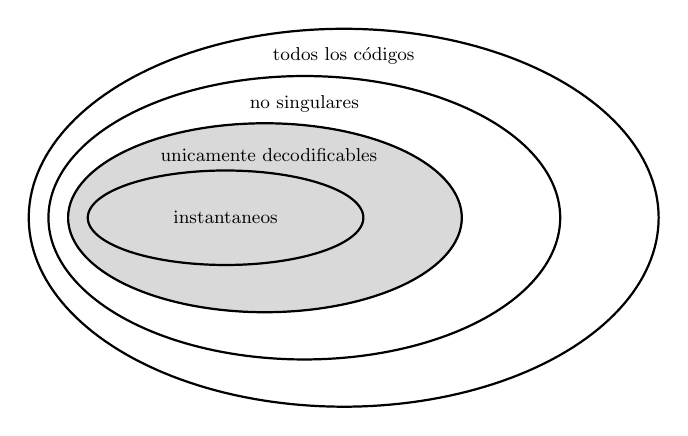
\begin{tikzpicture}
\shorthandoff{>}
\filldraw[fill=gray!30,domain=0:360, samples=200] plot ({2.5*cos(\x)+.5},{1.2*sin(\x)});
%%%%
\draw[thick,domain=0:360, samples=200] plot ({1.75*cos(\x)},{.6*sin(\x)});
\node[scale=.75] at (0,0){\small instantaneos};
%
\draw[thick,domain=0:360, samples=200] plot ({2.5*cos(\x)+.5},{1.2*sin(\x)});
\node[scale=.75] at (.55,.8){\small  unicamente decodificables};
%
\draw[thick,domain=0:360, samples=200] plot ({3.25*cos(\x)+1},{1.8*sin(\x)});
\node[scale=.75] at (1,1.45){\small no singulares};
%
\draw[thick,domain=0:360, samples=200] plot ({4*cos(\x)+1.5},{2.4*sin(\x)});
\node[scale=.75] at (1.5,2.05){\small todos los c\'odigos};
\end{tikzpicture}
 \end{center}
%
\leyenda{Clases  de c\'odigos.   Los  c\'odigos  contienen la  clase  de los  no
  singulares.  La misma  contiene la clase de los  c\'odigos descifrables.  Ella
  contiene los  c\'odigos instantaneos.  En  grise se representan las  clases de
  c\'odigos sin perdida a lo cuales se dedica esta secci\'on.}
%
\label{Fig:SZ:ClasesCodigos}
\end{figure}

Adem\'as  de   la  decodificaci\'on  sin   ambig\"uedad,  una  caracterizaci\'on
importante del  c\'odigo es la  taza de codificaci\'on~\footnote{En~\cite{Rio07}
  por  ejemplo, se  define esta  taza suponiendo  que cada  secuencia  fuente es
  codificada por el  mismo n\'umero de bits. La taza es  entonces el n\'umero de
  bits por s\'imbolo.}
%
\[
R_{c_m} = \frac{\log_d \left( \sum_{x \in \X^m} l(x) P(X = x) \right)}{m},
\]
%
donde $X$  representa una  secuencia de $m$  variables $X_t$.  El  argumento del
logaritmo (de base adecuada al cardenal  de $\C$) es el {\it largo promedio} del
c\'odigo. Por ejemplo,  para $d = 2$, $R_{c_m}$ es el  n\'umero de bits promedio
del c\'odigo por s\'imbolo.

En general,  se quiere minimizar $R_{c_m}$  (compresar el mensaje  a mandar), lo
que puede  ser contradictorio con la  necesidad de a\~nadir  redundancia para no
perder  informaci\'on   durante  una  transmisi\'on.   En  lo   que  sigue,  nos
concentramos en  el problema  de compresi\'on,  sin tener en  cuenta el  paso de
transmisi\'on  de  mensajes codificados  en  un  canal.   Minimizar la  taza  es
equivalente a minimizar el largo  promedio. Adem\'as, se puede focalisarse en $m
= 1$; todo se extiende sencillamente a $m > 1$.

La meta de  la compresi\'on es entonces construir  un c\'odigo $c$, descifrable,
que minimizar el largo promedio
%
\[
L(c) = \sum_{x \in \X} p_X(x) \, l(x).
\]
%
Antes de ir  m\'as adelante, hace falta traducir en  ecuaci\'on el v\'inculo que
$c$    sea    descifrable.    Eso    es    dado    por    la   desigualdad    de
Kraft-McMillan~~\cite{Kra49,   McM56,   Kar61}~\footnote{Esta  desigualdad   fue
  probabada  por  L.  G.   Kraft  para c\'odigos  instantaneos  en  su tesis  de
  maestria~\cite{Kra49}.  Luego, fue extendida  a los c\'odigos descifrables por
  B.  McMillan~\cite{McM56} (en  una nota de pie de pagina  de su papel, atribua
  esta  observaci\'on a J.   L.  Doob  hecha oralemente  durante una  escuela de
  verano en Ann Arbor, MI en agosto 1955).}
%
\begin{teorema}[Desigualdad de Kraft-McMillan]
\label{Teo:SZ:KraftMcMillan}
%
  Los largos  $l_c(x)$ de las palabras  c\'odigo de un  c\'odigo $c$ descifrable
  deben satisfacer la desigualdad
  %
  \[
  \sum_{x \in \X} d^{-l_c(x)} \le 1.
  \]
  %
  Rec\'iprocamente,  para cada  conjunto de  enteros $\{  \ell_x \}_{x  \in \X}$
  satisfaciendo  esta   desigualdad,  es   posible  de  construir   un  c\'odigo
  descifrable con $l_c(x) = \ell_x$.
\end{teorema}
%
\begin{proof}
  Para cualquier $k \ge 1$ y cualquiera  cadena $s = s_1 \cdots s_k \in \X^k$, la
  extensi\'on  del  c\'odigo,  $c_k(s_1  \cdots  s_k) =  c(s_1)  \cdots  c(s_k)$
  satisface $l_{c_k}(s) = \sum_{i=1}^k l_c(s_i)$. Entonces
  %
  \[
  \left(  \sum_{x  \in \X}  d^{-l_c(x)}  \right)^k \:  =  \:  \sum_{\bar{x} \in  \X^k}
  d^{-l_{c_k}(\bar{x})} \: = \: \sum_{m=1}^{k \, l_c^{\max}} \#(m) \, d^{-m},
  \]
  %
  re-escribiendo  la segunda  suma, agrupando  los t\'erminos  de  mismo largos,
  donde $\#(m)$  es el n\'umero de c\'odicos  de $\X^k$ teniendo el  largo $m$ y
  $l_c^{\max}  =  \max_{x  \in  \X}  l_c(x)$  es el  largo  mayor.   $c$  siendo
  descifrable,  $c_k$ debe  ser inyectiva,  imponiendo $\#(m)  \le d^m$  (no hay
  m\'as palabras de  largo $m$ que el cardenal  de $\C^m$), dando inmediatemente
  que necesariamente
  %
  \[
  \forall \,  k \in \Nset^*, \quad \sum_{x  \in \X} d^{-l_c(x)} \le  \left( k \,
    l_c^{\max}  \right)^{\frac1k} \quad  \Leftrightarrow \quad  \sum_{x  \in \X}
  d^{-l_c(x)} \le \min_{k \in \Nset^*} \left( k \, l_c^{\max} \right)^{\frac1k}.
  \]
  %
  Un estudio r\'apido de \  $u \mapsto \left( u \, l_c^{\max} \right)^{\frac1u}$
  \ para \  $u \ge 1$ \ y  teniendo en cuenta de que $l_c^{\max}  \le 1$ permite
  concluir  que el  m\'inimo  es igual  a  1, terminando  la  parte directa  del
  teorema.

  Rec\'iprocamente, sea  \ $\{ \ell_x  \}_{x \in \X}$  \ un conjunto  de enteros
  satisfaciendo la  desigualdad de Kraft-McMillan.  Se puede  agrupar los largos
  iguales y  clasificarlos. Sea \ $n_\ell$ \  los n\'umeros de largos  igual a \
  $\ell =  1 , \ldots  , \ell^{\max} \le  \alpha$.  Consideramos ahora  un arbol
  empezando con una ra\'iz, correspondiente a un largo $0$, que se divide en $d$
  ramas, correspondiente a los largos iguales  a $1$; a cada nudo se asocian las
  letras \  $\cod_1, \ldots , \cod_d$. Esto  nudos se dividen cada  uno en $d$
  otras  ramas, y  los nudos  de ``padre''  \ $\cod_i$  \ se  va a  asociar las
  palabras c\'odigos \ $\cod_i \cod_1 , \ldots , \cod_i \cod_\alpha$, \ etc.
  Este  arbol,  conocido  como  arbol  de  Kraft,  es  ilustrado  en  la  figura
  Fig.~\ref{Fig:SZ:ArbolKraft}  para \  $d =  2$  \ y  \ $\C  =  \{0 \,  , \,  1
  \}$. Claramente, \ $n_1 \le d$ \ si no \ $n_1 \, d^{-1} > 1$ \ y los largos no
  podr\'ian  satisfacer  la  desigualdad  de Kraft-McMillan.   El  principio  es
  entonce de asociar a los \ $n_1$ \ (posiblemente igual a 0) largos iguales a \
  $1$ \ unos nudos con las palabras c\'odigo asociadas de largo \ $1$ \ (primera
  profundez  de  ramas)  y de  prohibir  todos  las  ramas  de padre  los  nudos
  seleccionados        (lineas        punteadas        en       la        figura
  Fig.~\ref{Fig:SZ:ArbolKraft}). Estos  nudos son  llamados {\em hojas}  (no hay
  ramas).  En  la capa de ``hijos'' de  profundez/largos \ $2$, quedan  \ $d^2 -
  n_1 \, d$ \ nudos (accessibles)  que se pueden dividir en ramas.  Nuevamente, \
  $n_2 \le d^2 - n_1 \, d$ \  sino tendr\'iamos \ $n_1 \, d^{-1} + n_2 \, d^{-2}
  > 1$, \ incompatible con la  desigualdad de Kraft-McMillan. Se puede asociar a
  los \ $n_2$  \ largos iguales a \  $2$ \ unos nudos con  las palabras c\'odigo
  asociadas de  largo \ $2$  \ (segunda profundez),  y de prohibir que  salen de
  estos nudos  nuevas ramas (son entonces  hojas en la  segunda profundez), etc.
  Haciendo as\'i, se asocia un c\'odigo \  $c$ \ de largos \ $l_c(x) = \ell_x$ \
  que aparece libre  de prefijo, es decir instantaneo.   Entonces, este c\'odigo
  es tambi\'en descifrable.
\end{proof}

A este punto, se menciona los hechos siguientes
%
\begin{itemize}
\item  Los  largos de  un  c\'odigo  descifrable  satisfacen la  desigualdad  de
  Kraft-McMillan,  pero con  el  conjunto de  largos  correspondientes se  puede
  siempre  construir un c\'odigo  instantaneo.  Claramente,  se puede  buscar un
  c\'odigo de largo promedio m\'inimo  en los c\'odigos instantaneo, sin perdida
  de optimalidad (buscar en la clase  m\'as amplia de los descifrable no permite
  bajar el largo promedio).
%
\item En  los c\'odigos  libres de prefijo,  si se  fija el n\'umero  de hojas
  (\'ultima   profundez)  borradas   contruyendo  un   c\'odigo,  este   vale  \
  $\sum_{i=1}^{\ell^{\max}}  n_i  \,  d^{\ell^{\max}  -  i} =  \sum_{x  \in  \X}
  d^{\ell^{\max} -  l_c(x)}$.  \ Es  necesariamente menor que el  n\'umero total
  $d^{\ell^{\max}}$  de hojas,  lo  que  prueba el  teorema  para los  c\'odigos
  instantaneos~\cite{Kra49, Kar61}.
%
\item El teorema  se generaliza obviamente para codificar  una fuente (discreta)
  con un n\'umero infinito de estados, tomando el l\'imite $\alpha \to \infty$.
%
\item Si se conocen los largos  \'optimos, es suficiente para poder construir un
  c\'odigo libre de prefijo.
\end{itemize}

\begin{figure}[h!]
%
\begin{center} 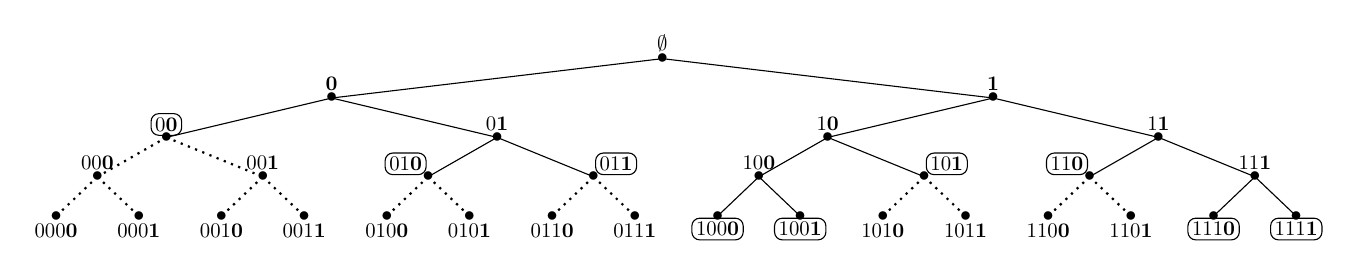
\begin{tikzpicture}[xscale=1.4]
\shorthandoff{>}
%
% nivel 2^4
%%%%%%%%%%%%
\draw[thick,dotted] (.375,.5)--(0,0) node[scale=.8]{$\bullet$} node[below,scale=.75]{000\textbf{0}};
\draw[thick,dotted] (.375,.5)--(.75,0) node[scale=.8]{$\bullet$} node[below,scale=.75]{000\textbf{1}};
\draw[thick,dotted] (1.875,.5)--(1.5,0) node[scale=.8]{$\bullet$} node[below,scale=.75]{001\textbf{0}};
\draw[thick,dotted] (1.875,.5)--(2.25,0) node[scale=.8]{$\bullet$} node[below,scale=.75]{001\textbf{1}};
\draw[thick,dotted] (3.375,.5)--(3,0) node[scale=.8]{$\bullet$} node[below,scale=.75]{010\textbf{0}};
\draw[thick,dotted] (3.375,.5)--(3.75,0) node[scale=.8]{$\bullet$} node[below,scale=.75]{010\textbf{1}};
\draw[thick,dotted] (4.875,.5)--(4.5,0) node[scale=.8]{$\bullet$} node[below,scale=.75]{011\textbf{0}};
\draw[thick,dotted] (4.875,.5)--(5.25,0) node[scale=.8]{$\bullet$} node[below,scale=.75]{011\textbf{1}};
%
\draw (6.375,.5)--(6,0) node[scale=.8]{$\bullet$}
node[inner sep=2pt,outer sep=1pt,draw=black,below,scale=.75,rounded corners=1mm]{100\textbf{0}};
%
\draw (6.375,.5)--(6.75,0) node[scale=.8]{$\bullet$}
node[inner sep=2pt,outer sep=1pt,draw=black,below,scale=.75,rounded corners=1mm]{100\textbf{1}};
%
\draw[thick,dotted] (7.875,.5)--(7.5,0) node[scale=.8]{$\bullet$} node[below,scale=.75]{101\textbf{0}};
\draw[thick,dotted] (7.875,.5)--(8.25,0) node[scale=.8]{$\bullet$} node[below,scale=.75]{101\textbf{1}};
\draw[thick,dotted] (9.375,.5)--(9,0) node[scale=.8]{$\bullet$} node[below,scale=.75]{110\textbf{0}};
\draw[thick,dotted] (9.375,.5)--(9.75,0) node[scale=.8]{$\bullet$} node[below,scale=.75]{110\textbf{1}};
%
\draw (10.875,.5)--(10.5,0) node[scale=.8]{$\bullet$}
node[inner sep=2pt,outer sep=1pt,draw=black,below,scale=.75,rounded corners=1mm]{111\textbf{0}};
%
\draw (10.875,.5)--(11.25,0) node[scale=.8]{$\bullet$}
node[inner sep=2pt,outer sep=1pt,draw=black,below,scale=.75,rounded corners=1mm]{111\textbf{1}};
%
%----------
%
% nivel 2^3
%%%%%%%%%%%%
\draw[thick,dotted] (1,1)--(.375,.5) node[scale=.8]{$\bullet$} node[above,scale=.75]{00\textbf{0}};
\draw[thick,dotted] (1,1)--(1.875,.5) node[scale=.8]{$\bullet$} node[above,scale=.75]{00\textbf{1}};
%
\draw (4,1)--(3.375,.5) node[scale=.8]{$\bullet$}
node[inner sep=2pt,outer sep=1pt,draw=black,above left,scale=.75,rounded corners=1mm]{01\textbf{0}};
%
\draw (4,1)--(4.875,.5) node[scale=.8]{$\bullet$}
node[inner sep=2pt,outer sep=1pt,draw=black,above right,scale=.75,rounded corners=1mm]{01\textbf{1}};
%
\draw (7,1)--(6.375,.5) node[scale=.8]{$\bullet$} node[above,scale=.75]{10\textbf{0}};
%
\draw (7,1)--(7.875,.5) node[scale=.8]{$\bullet$}
node[inner sep=2pt,outer sep=1pt,draw=black,above right,scale=.75,rounded corners=1mm]{10\textbf{1}};
%
\draw (10,1)--(9.375,.5) node[scale=.8]{$\bullet$}
node[inner sep=2pt,outer sep=1pt,draw=black,above left,scale=.75,rounded corners=1mm]{11\textbf{0}};
%
\draw (10,1)--(10.875,.5) node[scale=.8]{$\bullet$} node[above,scale=.75]{11\textbf{1}};
%
%----------
%
% nivel 2^2
%%%%%%%%%%%%
\draw (2.5,1.5)--(1,1) node[scale=.8]{$\bullet$}
node[inner sep=2pt,outer sep=1pt,draw=black,above,scale=.75,rounded corners=1mm]{0\textbf{0}};
%
\draw (2.5,1.5)--(4,1) node[scale=.8]{$\bullet$} node[above,scale=.75]{0\textbf{1}};
\draw (8.5,1.5)--(7,1) node[scale=.8]{$\bullet$} node[above,scale=.75]{1\textbf{0}};
\draw (8.5,1.5)--(10,1) node[scale=.8]{$\bullet$} node[above,scale=.75]{1\textbf{1}};
%
%----------
%
% nivel 2^1
%%%%%%%%%%%%
\draw (5.5,2)--(2.5,1.5) node[scale=.8]{$\bullet$} node[above,scale=.75]{\textbf{0}};
\draw (5.5,2)--(8.5,1.5) node[scale=.8]{$\bullet$} node[above,scale=.75]{\textbf{1}};
%
%----------
%
% nivel 2^0
%%%%%%%%%%%%
\draw (5.5,2) node[scale=.8]{$\bullet$} node[above,scale=.75]{$\emptyset$};

\end{tikzpicture} \end{center}
%
\leyenda{Arbol de  Kraft en el  caso binario ($d  = 2$). La ra\'iz,  de c\'odigo
  $\emptyset$ de largo 0, se divide en dos ramas, de c\'odigos respectivamente \
  $0$ \ y  \ $1$ \ (profundez \  $1$). Cada nudo de esta profundez  se divide en
  dos ramas (profundez dos), dando cuatros nuevos nudos con los c\'odigos \ $00$
  \ y $01$ de padre \ $0$, y \ $10$ \ y $11$ de padre \ $1$.  Etc.  En cada nudo
  de esta figura,  en el c\'odigo, se marca en  negrita la letra correspondiente
  al bit a\~nadido al c\'odigo padre.   Para hacer un c\'odigo libre de prefijo,
  una vez que un nudo es  seleccionado para ser una palabra c\'odigo (encuadrado
  en la  figura), no  puede tener nudos  ``hijos'' siendo tambi\'en  una palabra
  c\'odigo:  se boran  las ramas  saliendo  de un  nudo-palabra c\'odigo  (ramas
  punteadas).}
%
\label{Fig:SZ:ArbolKraft}
\end{figure}

El formalismo dado,  se va a ver ahora reaparecer la  entrop\'ia de Shannon como
cota de la codificaci\'on de fuente sin perdida:

\begin{teorema}[Cota inferior de c\'odigos descifrables]
\label{Teo:SZ:CotaInferiorCodigosDescifrables}
%
  Para  cualquier c\'odigo  \  $c$ \  descifrable  de la  fuente  $X$, su  largo
  promedio es  acotado por debajo  por la entrop\'ia  de Shannon de base  $d$ de
  $X$,
  %
  \[
  L(c) = \sum_{x \in \X} p_X(x) \, l_c(x) \: \ge \: H_d(X).
  \]
\end{teorema}
%
\begin{proof}
  Sea \ $q(x)  = \frac{d^{-l_c(x)}}{\sum_{x \in \X} d^{-l_c(x)}}$,  \ siendo una
  distribuci\'on de  probabilidad por  construcci\'on.  Escribiendo \  $l_c(x) =
  \log_d d^{-l_c(x)}$, \ se puede expresar el largo promedio de la forma
  %
  \[
  L(c) =  - \sum_{x  \in \X}  p_X(x) \, \log_d  d^{-l_c(x)} =  - \sum_{x  \in \X}
  p_X(x) \, \log_d q(x) - \log_d \sum_{x \in \X} d^{-l_c(x)}.
  \]
  %
  Notando que \ $- \log_d q  = \log_d \left( \frac{p_X}{q} \right) - \log_d p_X$
  \ se obtiene
  %
  \[
  L(c)  = H_d(X)  + D_{\mathrm{kl},d}\left(  \left.   p_X \right\|  q \right)  -
  \log_d \sum_{x \in \X} d^{-l_c(x)}.
  \]
  %
  El resultado proviene de la  positividad de la divergencia de Kullback-Leibler
  y de la desigualdad de Kraft-McMillan (el argumento del logaritmo siende menor
  que $1$).
\end{proof}
%
\noindent Este  resultado significa que la  taza de compresi\'on  sin perdida no
puede  ser m\'as  bajo que  el  contenido informacional  de la  fuente. En  este
sentido, $H$ tiene realmente un sabor de informaci\'on sobre la fuente $X$.

La entrop\'ia aparece tambi\'en en la cota superior del c\'odigo \'optimo:
%
\begin{teorema}[Cota superior del c\'odigo descifrable \'optimo]
\label{Teo:SZ:CotaSuperiorCodigoDescifrableOptimo}
%
  El largo promedio \ $L^\opt$ \ del c\'odigo \ $c^\opt$ \ descifrable, de largo
  promedio m\'inimo es  acotado por arriba por la entrop\'ia  de Shannon de base
  $d$ de $X$ m\'as un {\it dit} (1 s\'imbolo de $\C$),
  %
  \[
  L^\opt \: < \: H_d(X) + 1.
  \]
\end{teorema}
%
\begin{proof}
  Por  eso,  empezamos  por  buscar  los  largos  \'optimos,  soluci\'on  de  la
  optimizaci\'on
  %
  \[
  \min \sum_{x \in \X} p_X(x) \,  l(x) \qquad \mbox{sujeto a} \qquad \sum_{x \in
    \X} d^{-l(x)} \, \le \, 1.
  \]
  %
  %Sea \ $q(x)  = \frac{d^{-l_c(x)}}{\sum_{x \in \X} d^{-l_c(x)}}$,  \ siendo una
  %distribuci\'on de  probabilidad por  construcci\'on.  
  Escribiendo  \ $l_c(x) =  \log_d d^{-l_c(x)}$,  \ se  puede expresar  el largo
  promedio de la forma
  %
  \[
  L(c) =  - \sum_{x  \in \X}  p_X(x) \, \log_d  d^{-l_c(x)} =  - \sum_{x  \in \X}
  p_X(x) \, \log_d q(x) - \log_d \sum_{x \in \X} d^{-l_c(x)}.
  \]
  %
  Olvidando que los  \ $l_i \equiv l_c(x_i)$ \ son enteros,  $L(c)$ es convexa con
  respecto  a los $l_i$  as\'i que  el v\'inculo,  garantizando que  el m\'inimo
  existe y es \'unico.  El problema se resuelva con el enfoque KKT (Ver
    nota de pie~\ref{Foot:SZ:KKT}),
  % pagina~\pageref{Foot:SZ:KKT}.}, 
    optimizaci\'on  con  v\'inculos  tipo desigualdades~\cite{Mil00,  CamMar09},
    conduciendo a los ``largos''
  %
  \[
  \widetilde{l}(x) = - \log_d p_X(x).
  \]
  %
  $\widetilde{l}(x)$ no es necesariamente entero, as\'i que una posibilidad para
  volver  a largos  enteros  puede ser  de  tomar la  parte  entera superior  de
  $\widetilde{l}(x)$,
  %
  \[
  l(x) = \Big\lceil\! - \log_d p_X(x) \Big\rceil.
  \]
  %
  Obviamente el  conjunto de largos satisface la  desigualdad de Kraft-McMillan,
  as\'i que  se puede construir un  c\'odigo \ $c^\sh$ \  descrifrable con estos
  largos. De \ $l(x) < - \log_d p_X(x) + 1$ se obtiene
  %
  \[
   L^\opt \le L\left( c^\sh \right) < H_d(X) + 1.
  \]
  %
\end{proof}
%
De \[  H_d(X) \le  L^\opt < H_d(X)  + 1 \]  se revela  el rol fundamental  de la
entrop\'ia en la  codificaci\'on de fuente sin perdida.   La codificaci\'on es a
veces  dicha {\it  codificaci\'on  entr\'opica} y  da  un rol  operacional a  la
entrop\'ia  de  Shannon.   Se   notar\'a  tambi\'en  que  de  la  demostraci\'on
precediente  de   que  aparece  un   c\'odigo  particular  a  trav\'es   de  los
$\Big\lceil\!  - \log_d p_X(x) \Big\rceil$:
%
\begin{definicion}[C\'odigo de Shannon]
\label{Def:SZ:ShannonCode}
%
  Un  c\'odigo  \  $c^\sh$  \  de  una  fuente $X$,  de  largos  \  $l^\sh(x)  =
  \Big\lceil\!   - \log_d  p_X(x) \Big\rceil$,  \ libre  de  prefijo (construido
  sobre el arbol de Kraft) es llamado {\it c\'odigo de Shannon}.
\end{definicion}
%
Obviamente, tambi\'en
%
\[
H_d(X) \le L\left( c^\sh  \right) < H_d(X) +  1.
\]
%
Al lo contrario de primer vista, un  c\'odigo de Shannon no es \'optimo, como se
lo puede ver con el ejemplo siguiente.
%
\begin{ejemplo}
\label{Ej:SZ:CodigoShannonNoOpt}
%
  Sea \ $\X  = \C = \{ 0 \,  , \, 1 \}$ \  y una fuente $X$ tal que  \ $p_X(0) =
  0.999 = 1 - p_X(1)$.   Los largos de Shannon van a ser \ $l^\sh(0)  = 1$ \ y \
  $l^\sh(1) = 10$,  y el largo promedio vale \ $L\left(  c^\sh \right) = 1.009$.
  Obviamente, un c\'odigo \'optimo es \ $c(x) =  x$ \ de largos \ $l_c(x) = 1$ \
  dando \ $L^\opt = 1$ bit.
\end{ejemplo}
%
De hecho, volviendo al problema  con largos virtualmente no enteros, el m\'inimo
se alcanza para  $\widetilde{l}(x) = - \log_d p_X(x)$, es  decir que, los largos
siendo enteros, se alcanza la cota m\'inima del c\'odigo \'optimo si y solamente
si $- \log_d p_X(x)$.  Una distribuci\'on satifaciendo esta condici\'on es dicha
$d$-\'adica.   Sin embargo,  el c\'odigo  de  Shannon es  ``competitivo'' en  el
sentido de que:
%
\begin{teorema}[Competitividad del c\'odigo de Shannon]
\label{Teo:SZ:CompetitividadCodigoShannon}
%
Sea  $X$ \ fuente  sobre \  $\X$, de  distribuci\'on \  $p_X$ \  y \  $c^\sh$ el
c\'odigo de Shannon asociado  sobre el alfabeto c\'odigo \ $\C =  \{ \cod_1 \, ,
\,  \ldots \, ,  \, \cod_d  \}$, de  largos $l^\sh(x)  = \Big\lceil\!   - \log_d
p_X(x) \Big\rceil$.  Para cualquier c\'odigo  \ $c$ \ descifrable y cualquier $k
\ge 1$,
  %
  \[
  P\Big( l^\sh(X) \ge l_c(X) + k \Big) \le \frac{1}{d^{k-1}}.
  \]
\end{teorema}
%
\begin{proof}
  Por definici\'on de la parte entera superior, $a + 1 > \lceil a \rceil$, as\'i
  que $\lceil a \rceil \ge b \: \Rightarrow \: a > b-1$. A continuaci\'on, de la
  implicaci\'on de eventos $(Y  \ge a) \subset (Y \ge b-1)$ \  dando $P(A \ge a)
  \le P(Y \ge b-1)$ \ y de la definici\'on de un c\'odigo de Shannon se obtiene
  %
  \begin{eqnarray*}
  P\Big( l^\sh(X)  \ge l_c(X) + k  \Big) & \le & P\Big(  - \log_d p_X(X)
  \ge  l_c(X) + k  - 1  \Big)\\[2.5mm]
  %
  & = &  P\Big( p_X(X)  \le d^{-l_c(X)  - k  + 1} \Big)\\[2.5mm]
  %
  & = &  \sum_{x \in \X : p_X(x) \le d^{-l_c(x)  - k  + 1}} p_X(x)
  \end{eqnarray*}
  %
  Pero, sumando sobre  lo $x$ tal que $p_X(x) \le d^{-l_c(x)  - k + 1}$,
  se obtiene
  %
  \[
  P\Big( l^\sh(X)  \ge l_c(X) + k  \Big) \le \frac{1}{d^{k-1}} \sum_{x  \in \X :
    p_X(x) \le d^{-l_c(x) - k + 1}} d^{-l_c(x)}
  \le \frac{1}{d^{k-1}} \sum_{x \in \X} d^{-l_c(x)}
  \]
  %
  (a\~nadiendo t\'erminos positivos en la suma). La prueba se cierra notando que
  $c$ siendo descifrable, $l_c$ satisface la desigualdad de Kraft-McMillan.
\end{proof}
%
Este  teorema traduce  el hecho  que a  pesar de  que $c^\sh$  no  sea \'optimo,
tomando  cualquier otro c\'odigo,  incluyendo el  \'optimo, la  probabilidad que
$c^\sh(X)$ tenga un largo m\'as grande que $c(X)+k$ decrece exponencialmente con
$k$.
%
\begin{ejemplo}
\label{Ej:SZ:CompetitividadCodigoShannon}
%
  De manera general, con $d = 2$ y para $k = 9$, $P\Big( l^\sh(X) \ge l_c(X) + 9
  \Big)      \le       0.391      \%$.      En       particular,      en      el
  ejemplo~\ref{Ej:SZ:CodigoShannonNoOpt},    notando    que    s\'olo   en    la
  codificaci\'on de $x=1$ se puede tener $l^\sh(x) \ge l_c(x) + 9$, si no se usa
  1 bit, este resultado significa que la probabilidad de usar m\'as de 1 bit con
  el c\'odigo de Shannon es menor que $0.391 \%$. De hecho, una palabra c\'odigo
  de largo $10$ aparece con una probabilidad $0.1\%$\ldots
\end{ejemplo}

En el problema  de minimizaci\'on, el hecho que los largos  deben ser enteros no
permite solucionar explicitamente el problema de busqueda del c\'odigo \'optimo.
N\'umeros investigadores  contruyeron c\'odigos,  intentando probar de  que eran
\'optimos (ver  ej.~\cite{Sha48, ShaWea64,  Fan49} por los  primeros, y~\cite[\&
ref.]{CovTho06}).  El c\'odigo conocido  como {\it c\'odigo de Fano}~\footnote{A
  pesar  de que  sea  diferente del  de Shannon  y  que cada  uno fueron  hechos
  independientemente, a veces  es conocido como c\'odigo de  Fano-Shannon, o aun
  Shannon-Fano-Elias~\cite{CovTho06, KraLiu15}.}  \ $c^\fa$  \ se basa  sobre el
hecho de que se alcanza la cota m\'inima para una distribuci\'on $d$-\'adica.
%
\begin{definicion}[C\'odigo de Fano]
\label{Def:SZ:FanoCode}
%
  El  principio  es  de  clasificar   los  estados  de  $\X$  para  obtener  las
  probabilidades clasificadas en  orden decreciences ($p_X^\downarrow$).  Luego,
  se divide $\X$ en $d$ ensembles a  lo m\'as equiprobables que se puede (\ie de
  probabilidad a lo  m\'as cerca de $d^{-1}$) y de  asignar $\cod_i$ al conjunto
  $i$.   Luego,   se  repite  el   proceso  a  cada  sub-conjunto   (para  tener
  sub-conjuntos de probabilidades a lo m\'as cerca de $d^{-2}$) y al subconjunto
  $j$ del conjunto $i$ se va a asignar le c\'odigo $\cod_i \cod_j$, etc.  Eso es
  ilustrado en la figura Fig.~\ref{Fig:SZ:FanoHuffmanCodes}-(a).
\end{definicion}
%
\SZ{Probar/mencionar  que  tambi\'en  \[   H(X)  \le  L\left(  c^\fa  \right)  <
  H(X)+1. \]}
%  \qquad \mbox{con}  \qquad L^\fa  =  L_{c^\fa}$$}

Fijense de que no hay un \'unico c\'odigo  de Fano o de Shannon (tal como no hay
un \'optimo  \'unico).  Por exemple, hacer  una permutacion de  los $\cod_i$ da
los mismos  largos y  el mismo largo  promedio sin  cambiar el aspecto  libre de
prefijo. De la  misma manera, en el  arbol de Kraft, en cada  profundez se puede
permutar los s\'imbolos  asociados a las hojas de esta  profundez sin cambiar el
aspecto libre de  prefijo y sin que cambien los largos  $l(x_i)$ (y entonces con
el mismo largo promedio).

Una soluci\'on para construir un  c\'odigo \'optima fue propuesta por Huffman en
1951-1952~\cite{Huf52,  Pig03}~\footnote{De hecho,  Huffman  fue estudiantes  de
  maestria  de Fano,  trabajando  en el  MIT.  Su  tesis  era de  probar que  el
  c\'odigo de Fano  era \'optimo: Huffman propus\'o su  propio c\'odigo, andando
  al rev\'es del enfoque de Fano, y demostr\'o que era \'optimo~\cite{Sti91}.}
%
\begin{definicion}[C\'odigo de Huffman]
\label{Def:SZ:HuffmanCode}
%
  Suponemos que  existe un $\beta \in  \Nset$ tal que~\footnote{Si  no, se puede
    elegir $\beta =  \left\lceil \frac{\alpha-d}{d-1} \right\rceil$, y completar
    $\X$  con  $d  +  \beta  (d-1)  -  \alpha$  s\'imbolos  fuente  fictivos  de
    probabilidades ceros, lo  que no va a cambiar ni la  entrop\'ia, ni el largo
    promedio del  c\'odico aferente.}   $\alpha =  |\X| = d  + \beta  (d-1)$. El
  algoritmo de Huffman consiste a construir un arbol donde cada nudo es asociado
  a un conjunto de s\'imbolos fuente y una letra de $\C$ de la manera siguiente:
  %
  \begin{enumerate}
  \item\label{Huffman:clasificar}   Clasificar  las   probabilidades   en  orden
    decrecientes: por cambio de escritura, llamamos \ $p_i$ \ las probabilidades
    rearregladas, y \ $x_i$ \ los s\'imbolo fuente correspondientes.
  %
  \item\label{Huffman:codigolocal}  A  cada \  $x_i,  \:  \alpha-d+1  \le i  \le
    \alpha$ ($d$  probabilidades m\'as debiles), \  associar un nudo  y la letra
    ``hijo'' \ $\cod_i$.
  %
  \item\label{Huffman:padre} Crear \ $d$ \ ramas saliendo de un nudo padre hasta
    los $d$ nudos $x_i, \: \alpha-d+1 \le i \le \alpha$.
  %
  \item\label{Huffman:reconfiguracion}  Crear un  nuevo  conjunto de  s\'imbolos
    fuente  \  $\widetilde{x}_i   =  x_i,  \:  1  \le  i   \le  \alpha-d$  \  de
    probabilidades   respectivas    \   $\widetilde{p}_i   =   p_i$    \   y   \
    $\widetilde{x}_{\alpha-d+1} = \{  x_j, \: \alpha-d+1 \le j  \le \alpha \}$ \
    de probabilidad  \ $\widetilde{p}_{\alpha-d+1}  = p_{\alpha-d+1} +  \ldots +
    p_\alpha$.  El \'ultimo ``super-s\'imbolo'' fuente es asociado al nudo padre
    de la etapa~\ref{Huffman:padre}.
  %
  \item  Si   quedan  m\'as  de   un  (super-)s\'imbolo  fuente,  volver   a  la
    etapa~\ref{Huffman:clasificar}  con \  $p  \equiv \widetilde{p}$  \  y \  $x
    \equiv \widetilde{x}$.
  \end{enumerate}
  %
  Como descrito tratando del c\'odigo usando  el arbol de Kraft, se construye el
  arbol saliendo de las hojas, y  luego, el c\'odigo \ $c^\huf(x_i)$ \ se deduce
  saliendo de  la ra\'iz  del arbol as\'i  construido, agregando las  letras del
  camino que  llega hasta  la hoja  \ $x_i$.  \  Eso es  ilustrado en  la figura
  Fig.~\ref{Fig:SZ:FanoHuffmanCodes}-(b) en el caso binario.
\end{definicion}
%
Se mencionar\'a que  a cada etapa, el nuevo  conjunto de super-s\'imbolos fuente
contiene   exactamente   \  $d-1$   \   s\'imbolos   menos   que  a   la   etapa
precediente.  As\'i, con  \ $\alpha  = d  + \beta  (d-1)$ \  el  algoritmo tiene
exactamente \ $\beta+1$ \ bucles y  en cada profundez no hay ning\'un nudo vacio
en  el sentido  que  o  es una  hoja,  o es  un  nudo padre/prefijo  (quedar\'an
exactamente $d$ nudos a agregar a la ra\'iz en la \'ultima etapa).  Por exemplo,
con \ $d = 3$ \ si tuvieramos \ $\alpha = 4$, en la segunda etapa tendriamos $2$
estados  a juntar,  dando un  c\'odigo de  largos $2,  2, 2,  1$.   Empezando la
primera etapa  con la asociaciaci\'on de  $2$ estados, es decir  $3$ teniendo en
cuenta un estado fictivo  ($\alpha = 5$, $\beta = 1$) van  a quedar 3 estados en
la segunda etapa,  dando un c\'odigo de largos  $2, 2, 1, 1$, es  decir de largo
promedio m\'as peque\~no.

\begin{teorema}[\'Optimalidad del c\'odigo de Huffman]
\label{Teo:SZ:OptimalidadHuffman}
%
  El algoritmo de Huffman da un c\'odigo \ $c^\huf$ \ de largo promedio m\'inimo
  en  la  clase de  los  c\'odigos  descrifrables y  los  libre  de prefijo  (se
  recordar\'a que  con los  largos de c\'odigos  descifrables, siempre  se puede
  construir un c\'odigo  libre de prefijo), es decir \  $L^\opt = L\left( c^\huf
  \right)$.
\end{teorema}
%
\begin{proof}
  Una  prueba  es  dada  por  ejemplo en~\cite[Sec.~5.8]{CovTho06}  en  el  caso
  binario, pero la  extensi\'on para $d >  2$ es un poco m\'as  sutil. La prueba
  m\'as general  es dada  por Huffman~\cite{Huf52} y  se consigue  tambi\'en por
  parte en~\cite{Pig03}.   Suponemos que  $\beta \ge 1$  (sino, el  resultado es
  obvio). Las etapas son
  %
  \begin{itemize}
  \item Sean $j,  k$ dos indices. Si \  $c^\opt$ \ es un c\'odigo  \'optimo, y \
    $c$ \ un c\'odigo tal que \ $l(x_i) = l^\opt_i, \quad i \ne j , k, \quad l_j
    = l^\opt_k  \quad \& \quad  l_k = l^\opt_j$,  \ se obtiene  \ $0 \le  L(c) -
    L^\opt  = \sum_i p_i  \left( l_i  - l^\opt_i  \right) =  (p_j -  p_k) \left(
      l^\opt_k  - l^\opt_j  \right)$.   \  Entonces $p_j  >  p_k \:  \Rightarrow
    l^\opt_j \le l^\opt_k$.
  %
  \item Sea  $\eta$ el n\'umero  de s\'imbolos fuente  con un c\'odigo  de largo
    m\'aximo \ $l_{\max}$ \ y \ $\eta' = \min(\eta,d)$.  Del punto anterior, los
    $\eta$  s\'imbolos  con  palabra  c\'odigo  de largo  m\'aximo  son  los  de
    probabilidades m\'as peque\~nas.
  %
  \item  Como descrito  antes, se  puede permutar  las letras  c\'odigos  de una
    profundez del arbol de Kraft sin  cambiar ni el aspecto libre de prefijo, ni
    el largo promedio. Se puede entonces considerar el c\'odigo \'optimo tal que
    los  $\eta'$ s\'imbolos  de probabilidades  las m\'as  peque\~nas  tienen el
    mismo  nudo padre,  \ie solamente  la \'ultima  letra c\'odigo  cambia entre
    ellos.
  %
  \item  Suponemos que  \ $\eta'  = \eta  < d$.   \ Sea  una  ``super-fuente'' \
    $\X^{(2)}  =  \left\{  x^{(2)}_i  \right\}_{i=1}^{\alpha-\eta'+1}$ \  con  \
    $x^{(2)}_i  = x_i,  \quad  1 \le  i  \le \alpha-\eta'$  \ de  probabilidades
    respectivas  \  $p(x_i)$  \  y  \ $x^{(2)}_{\alpha-\eta'+1}  \equiv  \{  x_i
    \}_{i=\alpha-\eta'+1}^\alpha$  \  de  probabilidad \  $p_{\alpha-\eta'+1}  +
    \cdots   +  p_\alpha$   \   (se   ``plegan''  las   $\eta'$   hojas  en   un
    super-s\'imbolo).    La   c\'odificaci\'on    \'optima   es   entonces   una
    codificaci\'on libre de prefijo de $\X^{(2)}$, ``arbol ra\'iz'' del c\'odigo
    \'optimo, a la cual se a\~nade  una letra c\'odigo $\cod_j$ diferente a cada
    s\'imbolo  del  super-s\'imbolo  $x^{(2)}_{\alpha-\eta'+1}$.   La  profundez
    m\'axima del  c\'odigo arbol  es \ $l_{\max}-1$  \ y  debe ser llena,  en el
    sentido de que no debe tener un nudo que sea ni una hoja, ni un prefijo.  En
    el    caso   contrario,    se   podr\'ia    desplazar   un    s\'imbolo   de
    $x^{(2)}_{\alpha-\eta'+1}$ al  nudo ``vacio'' de  la profundez $l_{\max}-1$,
    sin cambiar  el aspecto  libre de prefijo,  pero ganando una  letra c\'odigo
    sobre un  s\'imbolo, \ie  hacer un  c\'odigo libre de  prefijo con  un largo
    promedio  menor.  Ser\'ia  contradictorio  con la  optimalidad del  c\'odigo
    inicial.
  % 
  \item  Para   c\'odificar  $\X^{(2)}$,  se  necesita  por   lo  menos  $\lceil
    \log_d(\alpha-\eta'+1)  \rceil$  profundez  en  el arbol  ra\'iz.   En  esta
    profundez   (m\'axima   en   el    caso   optimista),   hay   \   $d^{\lceil
      \log_d(\alpha-\eta'+1) \rceil} \ge \alpha-\eta'+1$ \ nudos. En la \'ultima
    profundez  pueden  ser  todos  ocupados  si  y  solamente  si  \  $d^{\lceil
      \log_d(\alpha-\eta'+1) \rceil}  = \alpha-\eta'+1$.  En  otras palabras, es
    posible si  y solamente si  existe un entero  $k$ tal que  $\alpha-\eta'+1 =
    d^k$, es decir, con \ $\alpha = d + \beta (d-1)$, \ que teniamos el entero \
    $\beta = \frac{d^k-d}{d-1} +  \frac{\eta'-1}{d-1}$.  \ La primera fracci\'on
    \ $\frac{d^k-d}{d-1}  = d^{k-1} +  \cdots + 1$  \ siendo entera,  $\beta$ no
    puede ser entero  con \ $\eta' < d$.  \  En otros t\'erminos, necesariamente
    $\eta' = d$, \ie los $d$  s\'imbolos de probabilidad m\'as debiles son el la
    \'ultima profundez y se puede elegir que comparten el mismo nudo padre.
  %
  \item Sea \ $c^{\opt,(1)}$ \ el c\'odigo \'optimo correspondiente a \ $\X$ \ y
    \ $c^{(2)}$  \ el  c\'odigo ``padre'' sobre  \ $\X^{(2)}$  \ ($c^{\opt,(1)}$
    quitando la \'ultimo  letra c\'odigo de los s\'imbolos  juntados, \ie con la
    ra\'iz  com\'un de  estos).  De  la misma  manera, sea  \  $c^{\opt,(2)}$ un
    c\'odigo  \'optimo sobre  $\X^{(2)}$ \  y \  $c^{(1)}$ \  el que  se obtiene
    deplegando el super-s\'imbolo \ $x^{(2)}_{\alpha-d+1}$ \ en $d$ hojas.  De \
    $L^{\opt,(1)}  =  L\left(  c^{(2)}  \right)  +  p_{\alpha-d+1}  +  \cdots  +
    p_\alpha$ \ (pasar de $\X^{(2)}$ a  $\X$ se a\~nade solo una letra palabra a
    los  s\'imbolos  del super-s\'imbolo)  \  y  \  $L\left( c^{(1)}  \right)  =
    L^{\opt,(2)}  + p_{\alpha-d+1} +  \cdots +  p_\alpha$ \  se obiene  \ $\Big(
    L^{\opt,(1)} - L\left( c^{(1)} \right)  \Big) + \Big( L^{\opt,(2)} - L\left(
      c^{(2)}  \right) \Big)  \: =  \: 0$.   \ Cada  t\'ermino  entre parentesis
    siendo positivo, valen necesariamente  cero (la suma de t\'erminos positivos
    vale cero si y solamente si  todos son nulos).  En conclusi\'on, \ $c^{(2)}$
    \  padre   de  \  $c^{\opt,(1)}$   \  queda  \'optimo,  \   $c^{(2)}  \equiv
    c^{\opt,(2)}$ \ (y \ $c^{(1)} \equiv c^{\opt,(1)}$).
  %
  \item Notando que \ $|\X^{(2)}| = \alpha - (\beta-1) (d-1)$, \ el razonamiento
    se   propaga  por   inducci\'on,  pasando   de  \   $c^{\opt,(k)}$  \   a  \
    $c^{\opt,(k+1)}$ \ juntando los $d$ super-s\'imbolos de probabilidades m\'as
    debiles,  hasta tener  un  super-s\'imbolo tendiendo  todos los  s\'imbolos,
    $\left| \X^{(K)} \right| = 1$, ra\'iz del arbol.
\end{itemize}
\end{proof}
%
De esta  prueba, se puede ver que
%
\begin{itemize}
\item  Cada  profundez siendo  llena,  los largos  obtenidos  van  a saturar  la
  desigualdad de Kraft-McMillan.
%
\item Si \ $\frac{\alpha  - d}{d-1}$ \ no es entero, en  lugar de completar $\X$
  con s\'imbolos fictivos se puede  empezar el algoritmo de Huffman juntando los
  \ $\alpha - d - \left\lfloor \frac{\alpha - d}{d-1} \right\rfloor (d-1) + 1$ \
  s\'imbolos fuentes  de probabilidades m\'as  debiles en un  super-s\'imbolo, y
  luego hacer el bucle descrito (juntando por super-s\'imbolos de $d$ s\'imbolos
  en  cada  bucle);  en  este  caso,  no  se  satura  m\'as  la  desigualdad  de
  Kraft-McMillan, pero  no es contradictorio  con el punto anterior  que contaba
  los largos de estados fictivos (que no codificamos en realidad).
%
\item Obviamente, en el caso binario $d = 2$, no es necesario completar $\X$ por
  estados fuentes, o  empezar con menos de $d$  s\'imbolos juntados ($\alpha$ es
  necesariamente de la forma $\alpha = d + \beta (d-1) = 2 + \beta$).
%
\item  El algoritmo  no  permite conocer  los  largos de  manera anal\'itica  en
  funci\'on  de $p_i$,  y  tampoco el  largo  promedio.  Se  los pueden  deducir
  solamente  implementando   el  algoritmo  (una   vez  que  es   construido  el
  c\'odigo). Era el caso tambi\'en con el enfoque de Fano.
\end{itemize}

Volviendo al c\'odigo  ingenuo, ser\'ia \'optimo (y equivalente a  los de Fano y
de Shannon) para una distribuci\'on uniforme. En este contexto, la entrop\'ia es
$H_d(X) = \log_d |\X|$, precisamente la incerteza del enfoque de Hartley
que   corresponde  a   los   n\'umeros  de   dits   necesarios  para   codificar
(ingenuosamente) la fuente.

\begin{figure}[h!]
\begin{center} 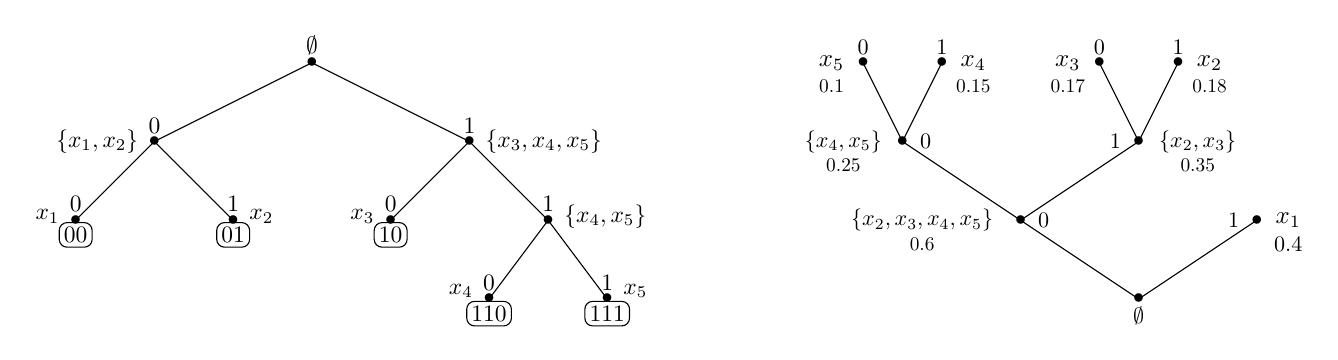
\begin{tikzpicture}%[xscale=3.5,yscale=3]
\shorthandoff{>}
%
% Codigo de Fano
\begin{scope}
\draw(0,0) node[scale=.8]{$\bullet$} node[above,scale=.85]{$\emptyset$};
%
% -----
%
\draw (0,0) -- (-2,-1) node[scale=.8]{$\bullet$} node[above,scale=.85]{$0$};
\draw (-2.1,-1) node[left,scale=.85]{$\{ x_1,x_2\}$};
%
\draw (0,0) -- (2,-1) node[scale=.8]{$\bullet$} node[above,scale=.85]{$1$};
\draw(2.1,-1) node[right,scale=.85]{$\{ x_3,x_4,x_5\}$};
%
% -----
%
\draw (-2,-1) -- (-3,-2) node[scale=.8]{$\bullet$} node[above,scale=.85]{$0$}
node[inner sep=2pt,outer sep=1pt,draw=black,below,scale=.85,rounded corners=1mm]{$00$};
\draw (-3.1,-1.95) node[left,scale=.85]{$\boldsymbol{x_1}$};
%
\draw (-2,-1) -- (-1,-2) node[scale=.8]{$\bullet$} node[above,scale=.85]{$1$}
node[inner sep=2pt,outer sep=1pt,draw=black,below,scale=.85,rounded corners=1mm]{$01$};
\draw (-.9,-1.95) node[right,scale=.85]{$\boldsymbol{x_2}$};
%
\draw (2,-1)-- (1,-2) node[scale=.8]{$\bullet$} node[above,scale=.85]{$0$}
node[inner sep=2pt,outer sep=1pt,draw=black,below,scale=.85,rounded corners=1mm]{$10$};
\draw (.9,-1.95) node[left,scale=.85]{$\boldsymbol{x_3}$};
%
\draw (2,-1)-- (3,-2) node[scale=.8]{$\bullet$} node[above,scale=.85]{$1$};
\draw (3.1,-1.95) node[right,scale=.85]{$\{ x_4 , x_5 \}$};
%
% -----
%
\draw (3,-2)-- (2.25,-3) node[scale=.8]{$\bullet$} node[above,scale=.85]{$0$}
node[inner sep=2pt,outer sep=1pt,draw=black,below,scale=.85,rounded corners=1mm]{$110$};
\draw (2.15,-2.9) node[left,scale=.85]{$\boldsymbol{x_4}$};
%
\draw (3,-2)-- (3.75,-3) node[scale=.8]{$\bullet$} node[above,scale=.85]{$1$}
node[inner sep=2pt,outer sep=1pt,draw=black,below,scale=.85,rounded corners=1mm]{$111$};
\draw (3.85,-2.9) node[right,scale=.85]{$\boldsymbol{x_5}$};
\end{scope}
%
%
% Codigo de Huffman
\begin{scope}[xshift=12cm]
\draw (-5,0) node[scale=.8]{$\bullet$} node[above,scale=.8]{$0$}
-- (-4.5,-1) node[scale=.8]{$\bullet$} node[right,scale=.8]{$\:\: 0$}
-- (-4,0) node[scale=.8]{$\bullet$} node[above,scale=.8]{$1$};
\draw(-5.4,0) node[scale=.9]{$\boldsymbol{x_5}$};
\draw(-5.4,-.3) node[scale=.7]{$0.1$};
\draw(-3.6,0) node[scale=.9]{$\boldsymbol{x_4}$};
\draw(-3.6,-.3) node[scale=.7]{$0.15$};
\draw(-5.25,-1) node[scale=.8]{$\{x_4,x_5\}$};
\draw(-5.25,-1.3) node[scale=.7]{$0.25$};
%
% -----
%
\draw (-2,0) node[scale=.8]{$\bullet$} node[above,scale=.8]{$0$}
-- (-1.5,-1) node[scale=.8]{$\bullet$} node[left,scale=.8]{$1\:\: $}
-- (-1,0) node[scale=.8]{$\bullet$} node[above,scale=.8]{$1$};
\draw(-2.4,0) node[scale=.9]{$\boldsymbol{x_3}$};
\draw(-2.4,-.3) node[scale=.7]{$0.17$};
\draw(-.6,0) node[scale=.9]{$\boldsymbol{x_2}$};
\draw(-.6,-.3) node[scale=.7]{$0.18$};
\draw(-.75,-1) node[scale=.8]{$\{x_2,x_3\}$};
\draw(-.75,-1.3) node[scale=.7]{$0.35$};
%
% -----
%
\draw (-4.5,-1) -- (-3,-2) node[scale=.8]{$\bullet$} node[right,scale=.8]{$\:\: 0$} -- (-1.5,-1);
\draw(-4.25,-2) node[scale=.8]{$\{x_2,x_3,x_4,x_5\}$};
\draw(-4.25,-2.3) node[scale=.7]{$0.6$};
%
% -----
%
\draw (-3,-2) -- (-1.5,-3) node[scale=.8]{$\bullet$} node[below,scale=.8]{$\emptyset$}
-- (0,-2) node[scale=.8]{$\bullet$} node[left,scale=.8]{$1\:\:$};
\draw(.4,-2) node[scale=.9]{$\boldsymbol{x_1}$};
\draw(.4,-2.3) node[scale=.8]{$0.4$};
\end{scope}
\end{tikzpicture} \end{center}
%
\leyenda{Construcci\'on de  un c\'odigo binario  sobre $\C =  \{0 \, , \,  1 \}$
  asociado al vector de probabilidad $p_X = \protect\begin{bmatrix} 0.4 & 0.18 &
    0.17 & 0.15 & 0.1 \protect\end{bmatrix}^t$ sobre el arbol de Kraft.  En este
  caso, $H_2(X)  \approx 2.1514$\ (a): Enfoque  de Fano, saliendo  de la ra\'iz.
  En cada nudo, se menciona el conjunto de s\'imbolos que va a tener el c\'odigo
  correspondiente  (en negro  cuando  es un  solo  s\'imbolo).  Se  pasa de  una
  profundez  a la  otra  dividiendo los  conjunto  en sub-conjuntos  a lo  m\'as
  equiprobables.   Esta construcci\'on  da el  c\'odigo \  $c^\fa(x_1) =  00, \:
  c^\fa(x_2) = 01, \: c^\fa(x_3) = 10, \: c^\fa(x_4) = 110, \: c^\fa(x_5) = 111$
  \ de  largo promedio \ $L\left(  c^\fa \right) =  2.25$.  \ \ (b):  Enfoque de
  Huffman, saliendo de las hojas.   En cada nudo, se menciona el correspondiente
  (i) conjunto de s\'imbolos,  (ii) $\cod_i$ de esta profundez/posici\'on, (iii)
  la probabilidad  asociada al  conjunto.  Se  pasa de una  profundez a  la otra
  juntando  los conjuntos  menos  probables en  sobre-conjuntos.   En negro  son
  indicados los s\'imbolos simples: van a tener el c\'odigo agregando los de los
  nudos yendo de la ra\'iz hasta  las hojas.  Esta construcci\'on da el c\'odigo
  \ $c^\huf(x_1) = 1, \: c^\huf(x_2) = 011, \: c^\huf(x_3) = 010, \: c^\huf(x_4)
  = 001, \: c^\huf(x_5) = 000$ \ de largo promedio \ $L^\opt = 2.2$.}
%
\label{Fig:SZ:FanoHuffmanCodes}
\end{figure}


Se notar\'a  de que, tratando  de una fuente  \ $\{ X_t  \}_{t \in \Zset}$  \ de
variables independientes,  se puede  codificar la fuente  con un  largo promedio
arbitrariamente cerca  de $H_d(X)$.   El principio es  de considerar  vectores \
$\begin{bmatrix} X_1 & \cdots &  X_n \end{bmatrix}^t$ \ viviendo sobre \ $\X^n$,
llamado {\it extensi\'on de orden $n$ de la fuente}, con un c\'odigo descifrable
(o libre de  prefijo) de esta extensi\'on; es llamado  {\it codificaci\'on de la
  extensi\'on  de  la  fuente}  pero  no  es  necesariamente  una  extension  de
$c$. As\'i, \ $H_d(X_1 , \ldots ,  X_n) \le L^{\opt,n} < H_d(X_1 , \ldots , X_n)
+ 1$, es decir, de la independencia,
%
\[
H_d(X)  \:  \le \:  \frac{L^{\opt,n}}{n}  \: <  \:  H_d(X)  + \frac{1}{n}  \quad
\mbox{por s\'imbolo}
\]
%
(ver  tambi\'en~\cite[cap. 13,  teorema de  Shannon]{Rio07}). Fijense  que  si \
$\displaystyle   \lim_{n   \to  \infty}   \frac{L^{\opt,n}}{n}   \to  H(X)$,   \
$\frac{L^{\opt,n}}{n}$ \ no  es necesariamente decreciente con respeto  a \ $n$.
Eso  es descrito  figura Fig.~\ref{Fig:SZ:CodigosExtensiones}.   Lo  mismo puede
ocurir  con el c\'odigo  de Shannon  y lo  de Fano.   Adem\'as, el  cardenal del
alfabeto  extendido $\X^n$  crece exponencialmente  con $n$,  lo que  no permite
elegir un $n$ muy grande.

\begin{figure}[h!]
%
\begin{center} \begin{tikzpicture}
\shorthandoff{>}
%
%Axes
%\pgfmathsetmacro{\Hd}{-.34*log2(.34)-.66*log2(.66)}; % entropia para p = [.34 .66]
%
\draw[>=stealth,->] (.9,0)--(15.5,0) node[right]{\small $n$};
\draw[>=stealth,->] (1,-.1)--(1,2.5)
node[above,scale=.65]{$\displaystyle \frac{L^{\opt,n}}{n} - H_d(X)$};
\foreach \k in {1,...,15} {\draw (\k,0)--(\k,-.1) node[below,scale=.7]{\k};}
\draw (1,2)--(.9,2) node[left,scale=.7]{$1-H_d(X)$};
%
\draw[thin,color=gray!70] plot[mark=*,mark size=1.25, mark options={black}]
file {Data_SZ/Loptn_p033_libro.txt};
%\draw[thin,dashed] (-.1,\dec) node[left]{\small $H_d(X)$} --(12,\dec);
%\draw[thin,dashed] plot [domain=2:13,samples=100] (\x,{50/\x});
% ATTENTION, trace de (L-Hd) normalise puis double pour une question de lisibilite
\end{tikzpicture}
 \end{center}
%
\leyenda{$\frac{L^{\opt,n}}{n}-H_d(X)$  (puntos),   diferencia  entre  el  largo
  promedio \'optimo por s\'imbolo de las  extensiones \ $\X^n$ \ de orden $n$ de
  la fuente $\X$ y la cota inferior en funci\'on de $n$. La linea llena en grise
  sirve como gu\'ia. En esta ilustraci\'on se usa el ejemplo lo m\'as simple con
  \   $d   =   2$  \   y   \   $p   =   \protect\begin{bmatrix}  0.33   &   0.67
    \protect\end{bmatrix}^t$.}
%
\label{Fig:SZ:CodigosExtensiones}
\end{figure}

\

Para  codificar una  fuente, que  se haga  el c\'odigo  \'optimo de  Fano,  o de
Shannon,  hace  falta  usar  la  distribuci\'on de  probabilidad  de  la  fuente
$X$. Pr\'acticamente, es usual que no se la tiene. Frecuentemente, es estimada a
partir de datos,  o, dicho de otra manera, se  c\'odifica con una distribuci\'on
que no es la distribuci\'on verdadera de la fuenta. Una pregunta que surge es de
conocer lo que se pierde usando una distribuci\'on no adaptada (o ``falsa''). La
respuesta general  no es obvia, pero  tratando del c\'odigo de  Shannon se puede
contestar:

\begin{teorema}[C\'odigo falso de Shannon]
\label{Teo:SZ:CodigoFalsoShannon}
%
Sea $c^\sh(p)$  el c\'odigo  de Shannon sobre  el alfabeto  c\'odigo \ $\C  = \{
\cod_1 \, , \, \ldots \, ,  \, \cod_d \}$ asociado a la distribuci\'on $p$.  Sea
$X$  \  fuente  sobre  \  $\X$,  de  distribuci\'on  \  $p_X$  \  y  \  $q$  una
distribuci\'on cualquiera (ej.   estimada de $p_X$ presupuesta\ldots).  Entonces
el largo promedio  \ $L_{c^\sh(q)}$ \ del c\'odigo \ $c^\sh(q)$  \ aplicado a la
fuente \ $X$ \ satisface las desigualdades siguientes
  %
  \[
  H_d(p_X) +  D_{\mathrm{kl},d}\left( \left.  p_X \right\| q  \right) \:  \le \:
  L_{c^\sh(q)} \: < \: H_d(p_X)  + D_{\mathrm{kl},d}\left( \left. p_X \right\| q
  \right) + 1.
  \]
\end{teorema}
%
\begin{proof}
  Por definici\'on,
  \[
  L_{c^\sh}(q) = \sum_{x \in X} p_X(x) \, \Big\lceil\! -\log_d q(x) \Big\rceil.
  \]
  %
  La desigualdad viene de  \ $a \le \lceil a \rceil < a +  1$ \ y escribiendo $-
  p_X \log_d q = - p_X \log_d p_X + p_X \log \left( \frac{p_X}{q} \right)$.
\end{proof}
%
Olvidando el  posible extra dit (pensar  a la c\'odification  por bloques), este
teorema  da  una  interpretaci\'on  operacional  a  la  entrop\'ia  relativa,  o
divergencia  de  Kullback-Leibler.   Esta  cantidad  cuantifica  la  perdida  en
t\'ermino de largo  promedio codificando con una distribuci\'on  falsa. Dicho de
otra manera,  usando $q$  en lugar de  $p_X$, se  usa la informaci\'on  de $p_X$
porque se  c\'odifica la fuente $X$,  pero suponiendo la  distribuc\'ion $q$, se
piedre lo  que representa la  informaci\'on relativa de  $p_X$ con respeto  a la
referencia (distribuci\'on supuesta) $q$.

\

Existen varios otros  modos de codificar s\'imbolos. En  particular, con la meta
de transmitir los s\'imbolos codificados  en un canal de comunicaci\'on, a veces
no  es oportuno  de compresar  drasticamente  el mensaje.   Existen por  ejemplo
codificaciones que permiten una correcci\'on  de error en la recepci\'on. Pueden
tomar  en  cuenta  las  caracter\'isticas  del canal  de  transmisi\'on.   Estas
consideraciones  van m\'as  all\'a de  la ilustraci\'on  de esta  secci\'on.  El
lector puede referirse a~\cite{Ber74, Gal78, Say03, CovTho06, Rio07} entre otros
para tener m\'as detalles sobre varios esquemas de codificaci\'on/compresi\'on.

% R.  M.  Fano.  Class  notes  for Transmission  of  Information,  course  6.574
% (Technical Report). MIT, Cambridge, MA, 1952

%\SZ{Dire  un mot  sur  le codage  canal.   Cf avec  la  distribucion optimale  /
%  capacite cf. Elias 1954 - error free coding, Elias 1955 - error noisy channel,
%  Elias 57  - list  for decoding noisy  channels, Berlekamp (serie  papiers cles
%  dans les premiers).}

% ================================= Gaz perfecto

\subseccion{Gas perfecto}
\label{Ssec:SZ:GasPerfecto}

En el marco del gas perfecto

\SZ{Va donner un lien avec Boltzmann}


\

\SZ{Feder  Merhav  IT'94  et  lien  avec  discrimination;  Vacisek  en  test  de
  Gaussianite et cf plus loin avec generalises Gok75 etc}


% ============================== Generalizadas================================ %

\seccion{Entrop\'ias y divergencias generalizadas}
\label{Sec:SZ:Generalizadas}

\SZ{Partout, voir convexite stricte, en 1,  idem pour h monotone, etc. vis a vis
  des cas d'egalite avec les divergences.}

A pesar de  que la entrop\'ia de Shannon y  sus cantidades asociadas demostraron
sus  potencias  tan  de un  punto  de  vista  descriptivo  que en  t\'ermino  de
aplicaciones en la  transmisi\'on de la informaci\'on y  la compresi\'on, varias
nociones  informacionales, tipo entrop\'ias  o divergencias,  aparecieron luego.
En  esta  secci\'on  no  se  desarollar\'a  todos  los  enfoques  ni  todas  las
aplicaciones  tan  la literatura  es  importante. La  meta  es  dar los  caminos
conduciendo a las generalizaciones de la entrop\'ia de Shannon por un lado, y de
la divergencia de Kullback-Leibler por  el otro lado. No son siempre vinculados,
a pesar  de que sea  deseable que a  cada entrop\'ia sean asociados  nociones de
entrop\'ias condicionales y relativas.

% ================================= Salicru

\subseccion{Entrop\'ias y propiedades}
\label{Ssec:SZ:Salicru}

% ----- Entropias generalizadas particulares
%\paragraph{Unas  primeras  generalizaciones particulares}  
Si  la entrop\'ia  de Shannon  fue el  punto de  salida fundamental  en  todo el
desarollo  de la  teor\'ia de  la  informaci\'on, un  poco m\'as  de una  decada
despu\'es  de  su  papel  clave  y  muy completo,  R\'enyi  propuso  una  medida
generalizada~\cite{Ren61}.   Su  punto  de  vista  fue  m\'as  matem\'atico  que
f\'isico o ingeniero.  Retom\'o los axiomas de Fadeev~\cite{Fad56, Fad58, Khi57}
% Feinstein, cf ref  de R��nyi
%
para  probabilidades  incompletas~\footnote{En  esta  secci\'on, los  $p_i$  son
  componentes  del  vector  $p$   no  necesariamente  asociado  a  una  variable
  aleatoria; Hay  que entender de  que $p_i =  p_X(x_i)$ si son asociados  a una
  variable aleatoria $X$.}  $p = \begin{bmatrix} p_1 & \cdots & p_n
\end{bmatrix}^t,  \quad p_i  \ge  0,  \quad w_p  =  \sum_i p_i  \le  1$: (i)  la
invarianza de  $H(p)$ por permutaci\'on de  os $p_i$, (ii) la  continuidad de la
incerteza elemental  $H(p_i)$ ($p_i$ visto como  probabilidad incompleta), (iii)
$H\left( \frac12 \right) = 1 $,  (iv) la aditividad $H(p \otimes q) = H(p)+H(q)$
donde $p \otimes  q$ es el producto de  Kronecker o tensorial~\footnote{Ver nota
  de   pie~\ref{Foot:MP:Kronecker}   pagina~\pageref{Foot:MP:Kronecker}.},   \ie
probabilidad conjunta de dos variables independientes, y consider\'o en lugar de
la recursividad  un axioma  dicho de  valor promedio, axioma  muy parecido  a la
recursividad. Para $p$ \ y \ $q$ probabilidades incompletas tales que $p \, \cup
\, q = \begin{bmatrix} p_1 & \cdots  & p_n & q_1 & \cdots & q_m \end{bmatrix}^t$
sea incompleta  ($w_p +  w_q \le  1$), el  axioma (v) es  $H(p \,  \cup \,  q) =
\frac{w_p \, H(p) +  w_q \, H(q)}{w_p + w_q}$.  Demostr\'o que  con (v) en lugar
de la recursividad,  el conjunto de axiomas conduce de nuevo  a la entrop\'ia de
Shannon.  La generalizaci\'on propuesta por R\'enyi era de generalizar el axioma
(v) reemplazando la media aritm\'etica por una media generalizada (v') $H^\ren(p
\, \cup  \, q)  = g^{-1}  \left( \frac{w_p \,  g\big( H^\ren(p)  \big) +  w_q \,
    g\big( H^\ren(q) \big)}{w_p +  w_q}\right)$ con $g$ estrictamente mon\'otona
y  continua,  llamado  media  {\it  cuasi-aritm\'etica,  o  cuasi-lineal,  o  de
  Kolmogorov-Nagumo}.       De     las      propiedades     de      la     media
cuasi-aritm\'etica~\cite{Nag30,  Kol30, Kol91, HarLit52},  eso es  equivalente a
buscar una entrop\'ia elemental $H^\ren(p_i)$ y reemplazar la media aritm\'etica
\ $\sum_i  p_i H^\ren(p_i)$ por  una media de Kolmogorov-Nagumo,  $g^{-1} \left(
  \sum_i p_i g\big( H^\ren(p_i)  \big) \right)$.  R\'enyi propus\'o la funci\'on
de  Kolmogorov-Nagumo \  $g_\lambda(x) =  2^{(\lambda-1) x},  \quad  \lambda >0,
\quad \lambda  \ne 1$, probando  de que los axiomas  (i)-(ii)-(iii)-(iv)-(v') se
cumplen, conduciendo  a la  entrop\'ia de R\'enyi  de un vector  de probabilidad
$p$,
%
\[
H_\lambda^\ren(p) =  \frac{1}{1-\lambda} \log_2 \left(  \sum_{i=1}^n p_i^\lambda
\right).
\]
%
\noindent  Relaxando   el  axioma  (iii),   se  puede  elegir   $g_\lambda(x)  =
a^{(\lambda-1) x}, \quad a  > 0, \quad a \ne 1$; el  logaritmo ser\'a de la base
$a$ cualquiera. En  lo que sigue, usaremos $\log$ sin  precisar la elecci\'on de
base.   R\'enyi nombr\'o  esta  medida  de incerteza  {\it  entrop\'ia de  orden
  $\lambda$}. Notablemente,
%
\[
H_1^\ren(p)  \equiv   \lim_{\lambda  \to  1}  H_\lambda^\ren(p)   =  H(p)  \quad
\mbox{entrop\'ia de Shannon.}
\]
%
\noindent En otros t\'erminos, la clase de R\'enyi contiene como caso particular
la  entrop\'ia de  Shannon.   En su  papel,  R\'enyi introdujo  una ganancia  de
informaci\'on,  parecida  a una  entrop\'ia  relativa,  probando  que las  solas
entrop\'ias admisibles son  la de Shannon y la que  introdujo.  Volveremos en la
secci\'on siguiente  sobre esta entrop\'ia  relativa, o divergencia  de R\'enyi.
Por          axiomas,          las         propiedades~\ref{Prop:SZ:continuidad}
(continuidad),~\ref{Prop:SZ:permutacion}    (invarianza    por    permutaci\'on)
y~\ref{Prop:SZ:aditividad}  (additividad)   de  la  entrop\'ia   de  Shannon  se
conservan entonces en el marco de R\'enyi y se pierde~\ref{Prop:SZ:recursividad}
(recursividad), todav\'ia por axiomas. Veremos luego la otras que se conservan o
modifican en un marco m\'as general.

Unos a\~nos  despu\'es de R\'enyi, de  la famosa escuela  matem\'atica checa, J.
Havrda   \&    F.    Charv\'at   en~\cite{HavCha67}    (ver   tambi\'en~\cite[en
checo]{Vaj68}) volvieron a los axiomas de Khintchin, para extender la entopia de
Shannon,  \ie  considerando  (i)   la  invarianza  por  permutaci\'on,  (ii)  la
continuidad, (iii) la expansividad, (iv) $H^\hc(1) = 0$ y $H^\hc\left( \frac12 ,
  \frac12   \right)  =   1$,  pero   generalizando  la   recursividad   por  (v)
$H^\hc(p_1,\ldots,p_n)   =   H^\hc(p_1,\ldots,p_{n-2},p_{n-1}+p_n)   +   \lambda
(p_{n-1}+p_n)^\lambda         H^\hc\left(        \frac{p_{n-1}}{p_{n-1}        +
    p_p},\frac{p_n}{p_{n-1} + p_p} \right),  \quad \lambda > 0$~\footnote{En sus
  papel, lo imponen  para cualquier par $(p_i, p_j)$  sin imponer la invarianza
  por permutaci\'on, pero es equivalente  a la exposici\'on de este p\'arrafo.}.
Con $\lambda = 1$ se recupera la recursividad estandar, pero con $\lambda \ne 1$
eso permite dar un  peso diferente a la incerteza del estado  interno, \ie a las
probabilidades  que  se juntan  (la  describen  como clasificaci\'on  refinada).
Estos axiomas conducen necesariamente a la entrop\'ia (teorema~1 del papel)
%
\[
H_\lambda^\hc(p) = \frac{1}{1-2^{1-\lambda}} \left( 1 - \sum_i p_i^\lambda \right)
\]
%
que  nombraron {\it  $\lambda$-entrop\'ia structural}.   De nuevo,  relaxando el
axioma  (iv),   se  puede  reemplazar  en  el   coeficient  $2^{1-\lambda}$  por
$a^{1-\lambda}, \quad a > 0, \quad a \ne 1$. De nuevo, aparece que la entrop\'ia
de Shannon es un caso particular,
%
\[
H_1^\hc(p)  \equiv   \lim_{\lambda  \to   1}  H_\lambda^\hc(p)   =   H(p)  \quad
\mbox{entrop\'ia de Shannon.}
\]
%
Por axioma, se conservan las propiedades~\ref{Prop:SZ:continuidad} (continuidad)
y~\ref{Prop:SZ:expansabilidad}  (expansabilidad) de  Shannon en  este  marco. Se
prob\'o tambi\'en que se conserva la  propiedad de concavidad con respecto a los
$p_i$~\ref{Prop:SZ:concavidad},   la   de   maximalidad~\ref{Prop:SZ:cotamaxima}
alcanzada para una distribuci\'on uniforma (teorema~2). Aun que no aparece as\'i
en        el        papel,        satisface        la        propiedad        de
Schur-concavidad~\ref{Prop:SZ:Schurconcavidad}  (teorema~3).   A  pesar  de  que
mencionan que $H_\lambda^\hc$ sea diferente de $H_\lambda^\ren$, es sencillo ver
que hay un mapa uno-uno entre las dos entrop\'ias.  Se mencionar\'an en un marco
m\'as general otras propiedades de esta entrop\'ia.

Independiente de Havrda  \& Charv\'at, de la escuela h\'ugara  de la teor\'ia de
la informaci\'on,  Z.  Dar\'oczy en~\cite{Dar70} defin\'o la  entrop\'ia $H^f$ a
partir de una {\it funci\'on  informaci\'on} $f$ satifaciendo (i) $f(0) = f(1)$,
(ii) $f\left(\frac12\right) = 1$ \ y  la ecuaci\'on funcional (ii) $f(x) + (1-x)
f\left(  \frac{y}{1-x} \right)  = f(y)  + (1-y)  f\left(  \frac{x}{1-y} \right)$
sobre  $\{  (x,y)  \in [0  \;  1)^2,  \quad  x+y  \le  1 \}$,  siendo  $H^f(p)  =
\sum_{i=2}^n s_i  f\left( \frac{p_i}{s_i} \right), \quad  s_i = \sum_{j=1}^{i-1}
p_j$.   Dar\'oczy mostr\'o  que  si $f$  es medible,  o  continua en  $0$, o  no
negativa  y  acotada, necesariamente  $f(x)  =  h_2(x) =  -x  \log_2  x -  (1-x)
\log_2(1-x)$,   conduciendo  a   la  entrop\'ia   de  Shannon   (teorema~1;  ver
tambi\'en~\cite{Lee64, Tve58,  Ken64}).  En otros  t\'erminos, su axioma  (v) es
alternativa a la recursividad.  Para  extender la entrop\'ia de Shannon, propuso
extender  este   axioma  (v)  por   la  ecuaci\'on  funcional   $f_\lambda(x)  +
(1-x)^\lambda   f_\lambda\left(   \frac{y}{1-x}   \right)   =   f_\lambda(y)   +
(1-y)^\lambda   f_\lambda\left(   \frac{x}{1-y}   \right)$,   lo   que   condujo
necesariamente a la entrop\'ia (teoremas~2 y~3)
%
\[
H_\lambda^\dar(p) = \frac{1}{1-2^{1-\lambda}} \left( 1 - \sum_i p_i^\lambda \right),
\]
%
\noindent  es decir  nada  m\'as que  la  entrop\'ia introducida  por Havdra  \&
Charv\'at. En lo  que sigue, se la denotar\'a  $H_\lambda^\hcd$. Sin embargo, el
estudio  de  Dar\'oczy  fue m\'as  intensivo  que  el  de Havdra  \&  Charv\'at.
Primero, not\'o  el mapa entre su  entrop\'ia y la de  R\'enyi. Adicionalmente a
Havdra-Charv\'at prob\'o que  se conserva la propiedad~\ref{Prop:SZ:permutacion}
(invarianza  por   permutaci\'on,  que  no   era  un  axioma  en   su  enfoque),
$H_\lambda^\hcd\left( \frac12 , \frac12 \right) = 1$ (lo llama normalizaci\'on),
la  expansividad~\ref{Prop:SZ:expansabilidad},  una  aditividad  extendida,  una
recursividad extendida precisamente  del modelo de Havrda-Charv\'at (teorema~4).
Prob\'o  tambi\'en~\ref{Prop:SZ:positividad}, positividad  alcanzado en  el caso
determinista  y  la  maximalidad~\ref{Prop:SZ:cotamaxima}  en el  caso  uniforme
(teorema~6), que  incidentalmente $H_\lambda^\hcd\left( \frac1\alpha  , \ldots ,
  \frac1\alpha \right)$ crece con el  cardinal $|\X| = \alpha$.  Muy interesante
tambi\'en es que se puede definir  una entrop\'ia condicional en el mismo modelo
que en el  caso de Shannon, \ $H_\lambda^\hcd(X|Y)  = \sum_y \left[ p_{X|Y=y}(x)
\right]^\lambda  H_\lambda^\hcd(   p_{X|Y=y}  )$,   que  existe  una   regla  de
cadena~\ref{Prop:SZ:cadena},   $H_\lambda^\hcd(X,Y)    =   H_\lambda^\hcd(Y)   +
H_\lambda^\hcd(X|Y)$ y que condicionar reduce la entrop\'ia $H_\lambda^\hcd(X|Y)
\le    H_\lambda^\hcd(X)$    (teorema~8)~\ref{Prop:SZ:condicionar}.     Mostr\'o
tambi\'en que  si se  pierde la aditividad,  se obiene para  \ $X$  \ e \  $Y$ \
independientes \ $H_\lambda^\hcd(X,Y)  = H_\lambda^\hcd(X) + H_\lambda^\hcd(Y) +
\left(  2^{1-\lambda}  -  1  \right) H_\lambda^\hcd(X)  H_\lambda^\hcd(Y)$.   La
propiedades de regla  de cadena le permiti\'o revisitar  la caracterisaci\'on de
un canal de transmisi\'on y  redefinir una capacidad canal extendidas (capacidad
tipo $\lambda$;  basicamente se  usa el mismo  enfoque que Shannon,  pero usando
$H_\lambda^\hcd$ en lugar de $H$, ver secci\'on~6 del papel).

\

Las entrop\'ias  tipo Havdra-Charv\'at-Dar\'oczy fueron  (re)descubiertos varias
otras  veces  y/o estudiadas  m\'as  detenidamente  en  varios campos  y  varios
extensiones fueron  introducidas~\cite[entre otros]{Var66, Oni66,  Kap67, Vaj68,
  LinNie71,  Ari71,  Bur72,   AczDar75,  ShaMit75,  ShaMit75,  ShaTan75,  Mit75,
  BoeLub80, Fer80, Tsa88, Rat91, Kan01, Bec09}.  Un primer enfoque m\'as general
es debido a  S.  Arimoto en los primeros a\~nos  de la decada 1970~\cite{Ari71}.
Fue rediscubierto  y estudiado  con m\'as detalles  una decada despu\'es  por J.
Burbea y C.  R.  Rao~\cite{BurRao82} y luego por M.  Salicr\'u~\cite{Sal87} o M.
Teboulle~\cite{Teb92}   entre  otros.    La  medida   propuesta,   llamada  {\it
  $\phi$-entrop\'ia}, es definida por
%
\[
\hphi[p]  =   -\sum_i  \phi(p_i)  \qquad   \mbox{con}  \qquad  \phi   \:  \mbox{
  estrictamente convexa.}
\]
%
Burbea  y  Rao  asociaron una  medida  de  divegencia  a esta  entrop\'ia.   Las
$\phi$-entrop\'ias  contienen Shannon como  caso particular  ($\phi(x) =  x \log
x$),  as\'i que  la clase  de Havdra-Charv\'at-Dar\'oczy  ($\phi(x) =  \frac{x -
  x^\lambda}{2^{1-\lambda}-1}$) como mencionado, pero no la clase de R\'enyi. De
hecho, las  $\phi$-entrop\'ias se  enmarcan en una  clase un poco  m\'as amplia,
llamada {\it  $(h,\phi)$-entrop\'ias}~\cite{SalMen93, MenMor97}. Cambiamos ac\`a
substancialmente su escritura  de la literatura por razones  de homogeneidad con
la    $\phi$-entrop\'ia   (y    las   divergencias    que    se   introducir\'an
luego)~\footnote{En  la literatura,  no hay  el signo  $-$, y  hay  que invertir
  c\'oncava y convexa.}
%
\begin{definicion}[$(h,\phi)$-entrop\'ia]
\label{Def:SZ:HPhiEntropia}
%
  La $(h,\phi)$-entrop\'ia de una  distribuci\'on de probabilidad $p_X$ definida
  sobre $\X$ de cardinal finito $|\X| = \alpha$ es definida por
  %
  \[
  \hhphi[X] = \hhphi[p_X] = h\left(  - \sum_{x \in \X} \phi\left( p_X(x) \right)
  \right),
  \]
  %
  donde o
  %
  \begin{itemize}
  \item $\phi$ \ es estrictamente convexa y \ $h$ \ creciente, o
  \item $\phi$ \ es estrictamente c\'oncava y \ $h$ \ decreciente
  \end{itemize}
  %
  Frecuentemente, se supone adicionalmente que  $\phi$ y $h$ son de clase $C^2$,
  que $\phi(0) = 0$ (la incerteza elemental asociada a un estado de probabilidad
  nula vale cero) y, sin perdida de generalidad, que $h(-\phi(1)) = 0$.
\end{definicion}
%
\noindent  (ver  tambi\'en~\cite{Est97}  para  una  generalizaci\'on  aun  m\'as
amplia). Cu\'ando $h(x) = x$  se recupera la $\phi$-entrop\'ia, incluyendo la de
Shannon y las de Havdra-Charv\'at-Dar\'oczy. Adem\'as, la familia de R\'enyi cae
tamb\'ien en  esta familia  ($\phi(x) = -  x^\lambda$ \  y \ $h(x)  = \frac{\log
  x}{1-\lambda}$)  as\'i que  todas  las entrop\'ias  evocadas  en el  p\'arrafo
anterior.

Como   en   el   caso   de    Shannon,   para   $X   =   (X_1,\ldots,X_d)$,   la
$(h,\phi)$-entrop\'ia de $X$ es una $(h,\phi)$-entrop\'ia conjunta de los $X_i$.

Obviamente, de  las propiedades  de la entrop\'ia  de Shannon, se  conservan las
propiedades~\ref{Prop:SZ:continuidad}    (continuidad),~\ref{Prop:SZ:permutacion}
(invariaza    por   permutaci\'on),~\ref{Prop:SZ:biyeccion}    (invarianza   por
transformaci\'on       biyectiva      de      $X$),~\ref{Prop:SZ:expansabilidad}
(expansabilidad, debido a $\phi(0) = 0$).

Adem\'as  se conserva  la  Schur-concavidad \ con una reciproca:
%
\begin{propiedadesPhi}\setcounter{enumi}{\value{PropSchurConcavidad}}
%
\item Schur-convavidad:
  %
  \[
  p \prec q \quad \Longleftrightarrow \quad \hhphi[p] \ge \hhphi[q] \quad \forall \:
  (h,\phi).
  \]
  %
  En otros t\'erminos,  se obtiene la relaci\'on de  mayorisaci\'on si se cumple
  la  relaci\'on  de ordre  entr\'opicas  para  \underline{todos}  los pares  de
  funciones entr\'opicas  $(h,\phi)$.  La  Schur-concavidad (y su  reciproca) es
  consecuencia     de     la     desigualdad     de     Schur~\cite{Sch23}     o
  Hardy-Littlewood-P\'olya~\cite{HarLit29,   HarLit52}  o  Karamata~\cite{Kar32}
  (ver   tambi\'en~\cite[Cap.~3,  Prop.~C.1   \&   Cap.~4,  Prop.~B.1]{MarOlk11}
  o~\cite[Teorema~II.3.1]{Bha97}): $p \prec q \: \Rightarrow \: \sum_i \phi(p_i)
  \le \sum_i \phi(q_i)$ para toda funci\'on $\phi$ convexa, y reciprocamente.
\end{propiedadesPhi}
% Schur, I.  (1923). Issai Schur Collected  Works (A.  Brauer  and H.  Rohrbach,
% eds.), Vol. II. pp. 416����427. Springer-Verlag, Berlin, 1973]
%
%
% Ver Schur-Ostrowski f  sym, Schur-convexe ssi (xi - xj)  (df/dx_i - df/dxj) \ge
% 0, 1 \le i \ne j \le alpha
%
Como consecuencia, se  conservan la positividad~\ref{Prop:SZ:positividad} gracia
a \ $\phi(0) = 0$ \ y \ $h(-\phi(1)) = 0$ \ (alcanzado en el caso determinista),
la maximalidad~\ref{Prop:SZ:cotamaxima} (caso uniforme),
%
\[
0 \le \hhphi[p_X] \le h\left( - \alpha \, \phi\left( \frac1\alpha \right) \right),
\]
%
as\'i que
%
\[
\hhphi[\begin{bmatrix}  \frac1\alpha &  \cdots  & \frac1\alpha  \end{bmatrix}^t]
\quad \mbox{funci\'on creciente de } \alpha.
\]

Con respecto a la concavidad~\ref{Prop:SZ:concavidad}, no se conserva en general:
%
\begin{propiedadesPhi}\setcounter{enumi}{\value{PropConcavidad}}
\item\label{Prop:SZ:concavidadHPhi} Si $h$ es c\'oncava, entonces $\hhphi[p]$ es
  c\'oncava con  respecto a $p$.   Eso es una  consecuencia de la  concavidad de
  $\phi$ y  decrecencia de $h$ (resp.  convexidad/crecencia)  conjuntamente a la
  concavidad de $h$.  La reciproca no  es verdad.  Por ejemplo, se puede ver que
  si $\lambda  < 1$, la  entrop\'ia de R\'enyi  es c\'oncava, pero se  proba que
  existe  un  $\lambda^*(\alpha)  >  1$  tal que  para  cualquier  $\lambda  \le
  \lambda^*(\alpha)$  se conserva  la  concavidad, a  pesar  de que  $h$ no  sea
  necesariamente c\'oncava~\cite[p.~57]{BenZyc06}.
\end{propiedadesPhi}

Se pierde la propiedad de recursividad~\ref{Prop:SZ:recursividad}, pero se puede
vincular  la  entrop\'ia  total con  la  obtenida  juntando  dos estados  por  una
desigualdad:
%
\begin{propiedadesPhi}\setcounter{enumi}{\value{PropRecursividad}}
\item  Sean \  $X$  \ definido  sobre  \ $\X$  \  y \  $\breve{X}$  \ sobre  \
  $\breve{X}$,
  %
  \[
  \left\{  \begin{array}{l}\breve{\X}  = \{  x_1 \,  ,  \, \ldots \,  , \, x_{\alpha-2} \,  ,
      \, \breve{x}_{\alpha-1} \} \quad \mbox{con el estado interno} \quad
      \breve{x}_{\alpha-1}   =  \{   x_{\alpha-1} \,  , \,   x_\alpha  \},\\[2.5mm]
      p_{\breve{X}}(x_i) = p_X(x_i), \quad 1 \le i \le \alpha-1 \quad \mbox{y}
      \quad p_{\breve{X}}(\breve{x}_{\alpha-1}) = p_X(x_{\alpha-1}) +
      p(x_\alpha)  \quad  \mbox{distribuci\'on  sobre  }  \breve{\X}\\[2.5mm]
      \displaystyle   \breve{q}(x_j)  =   \frac{p_X(x_j)}{p_X(x_{\alpha-1})  +
        p_X(x_\alpha)},  \quad j =  \alpha-1, \alpha  \quad \mbox{distribuci\'on
        del estado interno}\end{array}\right.,
  \]
  %
  \[
  \hhphi[p_X] \ge \hhphi[p_{\breve{X}}].
  \]
  %
  Esta  desigualdad es  consecuencia de  la desigualdad  de Petrovi\'c~\cite[43,
  Teorema~8.7.1]{Kuc09}, $\phi(a + b) \ge \phi(a) + \phi(b)$ para $\phi$ convexa
  y que se cancela en 0 (y  la conversa en el caso c\'oncavo), conjuntamente con
  $h$ creciente  (resp.  decreciente).   Aparte en  el caso de  Shannon y  el de
  Havdra-Charv\'at-Dar\'oczy, no hay  ning\'un v\'inculo explicito general entre
  $\hhphi[p_X]$ \ y \ $\hhphi[p_{\breve{X}}]$.
\end{propiedadesPhi}

Se  conserva  la  super-aditividad~\ref{Prop:SZ:superaditividad}. De  hecho,  si
$\phi$ es convexa (resp.  c\'oncava) con \  $\phi(0) = 0$, \ $\forall \: 0 \le a
\le 1,  \: \phi(a u) =  \phi(a u + (1-a)  0) \le a  \phi(u)$ (resp.  desigualdad
reversa).   Entonces,  \   $\phi\left(  p_{X,Y}(x_i,y_j)  \right)  =  \phi\left(
  p_{X|Y=y_j}(x_i)  p_Y(y_j)  \right)  \le  p_{X|Y=y_j}(x_i)  \phi\left(p_Y(y_j)
\right)$, \ \ie \ $\sum_{i,j} \phi\left( p_{X,Y}(x_i,y_j) \right) \le \sum_{i,j}
p_{X|Y=y_j}(x_i) \phi\left(p_Y(y_j) \right) = \sum_i \phi\left(p_Y(y_j) \right)$
\  (resp.   desigualdad  reversa).   Se   cierra  la  prueba  con  la  crecencia
(resp. decrecencia) de $h$.


Sin  embargo, en  general, se  pierden  las propiedades~\ref{Prop:SZ:aditividad}
(aditividad), y~\ref{Prop:SZ:subaditividad}  (sub-aditividad). En particular, se
conserva solamente en el caso Shannon:
%
\begin{teorema}
\label{Teo:SZ:SoloShannonSubaditiva}
%
  Sea $p_{X,Y}$ distribuci\'on conjunta  de variables aleatorias discretas \ $X$
  \ y \ $Y$ \ y \ $p_X$ \ y \ $p_Y$ \ las de \ $X$ \ y de \ $Y$ (marginales).
  %
  \[
  \hhphi[p_{X,Y}] \:  \le \:  \hhphi[p_X \otimes p_Y]  \quad \forall  \: p_{X,Y}
  \qquad \Longleftrightarrow \qquad \phi(x) = x \log x,
  \]
  %
  \ie $\hhphi$ es una funci\'on creciente de la entrop\'ia de Shannon.
\end{teorema}
%
\begin{proof}
  La    reciproca     de    este    teorema    es    nada     m\'as    que    la
  propidad~\ref{Prop:SZ:subaditividad} con  el hecho de que $h$  es creciente en
  este caso.

  A continuaci\'on, la parte directa se demuestra en dos etapas:
  %
  \begin{itemize}
  \item Con  un caso particular  sobre $\X$  e $\Y$ de  cardenal 3 cada  unos se
    proba  de que  la desigualdad  no  se puede  cumplir, salvo  si la  derivada
    $\phi'$ de la funci\'on entr\'opica satisface a una ecuaci\'on funcional.
  %
  \item la sola soluci\'on admisible de esta ecuaci\'on se reduce a $\phi(x) = -
    x \ln x$.
  \end{itemize}
  %
  {\bf Etapa 1}: Sea el vector de probabildad
  %
  \[
  p_{X,Y}  =  p_X  \otimes   p_Y  -  c  \begin{bmatrix}  1\\-1\\0  \end{bmatrix}
  \otimes  \begin{bmatrix} 1\\-1\\0 \end{bmatrix}  \qquad \mbox{con}  \qquad p_X
  = \begin{bmatrix} a \\ \tilde{a} \\ 1-a-\tilde{a} \end{bmatrix} \quad \mbox{y}
  \quad p_Y = \begin{bmatrix} b \\ \tilde{b} \\ 1-b-\tilde{b} \end{bmatrix}
  \]
  %
  donde $(a,\tilde{a},b,\tilde{b}) \in D$,%_{a,\tilde{a},b,\tilde{b}}$,
  %
  \[
  %D_{a,\tilde{a},b,\tilde{b}} = \{  u, v, s, t:  \quad 0 < u,s <  1 \quad \&
  %\quad 0 < v \le 1-u \quad \& \quad 0 < t \le 1-s \},
  D =  \{ (u, \tilde{u},  v, \tilde{v}) \in  [0 \; 1]^4: \quad  0 <
    \tilde{u} \le 1-u \quad \& \quad 0 < \tilde{v} \le 1-v \},
  \]
  %
  y \ $c \in C_{a,\tilde{a},b,\tilde{b}}$,
  %
 \[
  C_{a,\tilde{a},b,\tilde{b}} = \big[ - 1 + \max\big\{ a b , \tilde{a} \tilde{b}
  , 1 - a \tilde{b} , 1 - \tilde{a}  b \big\} \, , \, \min\big\{ a b , \tilde{a}
  \tilde{b} , 1 - a \tilde{b} , 1 - \tilde{a} b \big\} \big].
  \]
  %
  Ahora, si $\phi$ es  convexa (resp. c\'oncava)
  %
  \[
  \forall \, u,v \quad \phi(v)  - \phi(u) \:  \ge \:  (v-u) \, \phi'(u),
  \]
  %
  \ie la  variaci\'on (cuerda) es mayor  que la derivada en  $u$, como ilustrado
  figura  Fig.~\ref{Fig:SZ:ConvexidadDerivada} (desigualdad reversa  para $\phi$
  c\'oncava).
  %
  \begin{figure}[h!]
  %
  \begin{center} 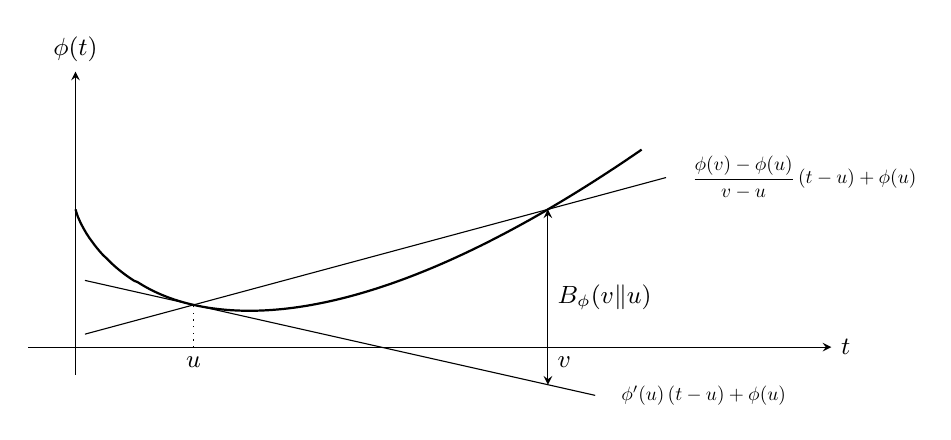
\begin{tikzpicture}
\shorthandoff{>}
%
% Concavidad de - u ln u
\begin{scope}[xscale=6,yscale=3.5]
\pgfmathsetmacro{\u}{.25};
\pgfmathsetmacro{\v}{1};
%
\draw[>=stealth,->] (-.1,-.5)--(1.6,-.5) node[right]{\small $t$};
\draw[>=stealth,->] (0,-.6)--(0,.5) node[above]{\small $\phi(t)$};
\draw[thick,domain=.005:1.2,samples=200] (0,0)-- plot (\x,{\x*ln(\x)});
\draw[dotted] (\u,-.5) node[below]{\small $u$} -- (\u,{\u*ln(\u)});
%\draw[dotted] (\v,-.55) node[below]{\small $v$} -- (\v,{\v*ln(\v)});
\draw[>=stealth,<->] (\v,{(1+ln(\u))*(\v-\u)+\u*ln(\u)}) -- (\v,{\v*ln(\v)});
\draw (\v,-.5) node[below right]{\small $v$};
\draw (\v,{.5*((1+ln(\u))*(\v-\u)+\u*ln(\u)+\v*ln(\v))}) 
node[right]{\small $B_\phi(v\|u)$};
%
\draw (.02,{(.02-\u)*(\v*ln(\v)-\u*ln(\u))/(\v-\u)+\u*ln(\u)})
-- (1.25,{(1.25-\u)*(\v*ln(\v)-\u*ln(\u))/(\v-\u)+\u*ln(\u)})
node[right,scale=.7]
{$\displaystyle \quad \frac{\phi(v)-\phi(u)}{v-u} \, (t-u) + \phi(u)$};;
%
\draw (.02,{(1+ln(\u))*(.02-\u)+\u*ln(\u)})--
(1.1,{(1+ln(\u))*(1.1-\u)+\u*ln(\u)})
node[right,scale=.7]{$\quad \phi'(u) \, (t-u) + \phi(u)$};
\end{scope}
%
%
% % Concavidad / mezcla
% \begin{scope}[xshift=8.5cm]
% \draw(0,1.25) node{\includegraphics[width=3cm]{TIKZ_SZ/DosDados}};
% \draw(-.5,2.5) node{\small $p_1$};
% \draw(1,2) node{\small $p_2$};
% \draw(2.7,1) node{\small $\lambda p_1 + (1-\lambda) p_2$};
% \draw(-.25,-1) node{\includegraphics[width=1cm]{TIKZ_SZ/Moneda}};
% \draw[>=stealth,->,thick] (-.3,-.35)--(-.75,.45);
% \draw (-.525,0) node[left]{\small $\lambda$};
% \draw[>=stealth,->,thick] (-.2,-.35)--(.3,.45);
% \draw (.05,0) node[right]{\small $1-\lambda$};
% \end{scope}
% %
% \draw (1.25,-2.25) node{(a)};
% \draw (8.25,-2.25) node{(b)};
\end{tikzpicture} \end{center}
  %
  \leyenda{$\phi$ estrictamente convexa:  la variaci\'on (cuerda) $\frac{\phi(v)
      -  \phi(u)}{v-u}$ es  mayor que  la derivada  $\phi'(u)$.  Aplicado  a dos
    distribuciones $p$ y $q$, de componentes $p_i$ y $q_i$, con $u = p_i$ y $v =
    q_i$  y  sumando, se  obtiene  $\hphi[q]  -  \hphi[p] \ge  \sum_i  (p_i-q_i)
    \phi'(p_i)$ con $\hphi \equiv H_{(\id,\phi)}, \: \id$ siendo la identidad.}
  %
  \label{Fig:SZ:ConvexidadDerivada}
  \end{figure}
  %
  Aplicamos esta desigualdad a \ $u =  p_{X,Y}(x,y)$ \ y \ $v = p_X(x) p_Y(y)$ \
  y sumamos  en $x,  y$, \  para \  $(a,b) \in (  0 \;  1)^2$ \  (para que
  $C_{a,\tilde{a},b,\tilde{b}}$  \ no  sea reducido  a \  $\{0\}$), y  \  $c \in
  \mathring{C}_{a,\tilde{a},b,\tilde{b}}$ \ donde  \ $\mathring{\cdot}$ \ denota
  el interior de un conjunto, se obtiene para $\phi$ convexa,
  %
  \[
  \hphi[p_X    \otimes   p_Y]    -    \hphi[p_{X,Y}]   \:    \le    \:   c    \:
  g(a,\tilde{a},b,\tilde{b},c)
  \]
  %
  (para $\phi$  c\'oncava se  reemplaza $\hphi$ por  $-H_{-\phi}$ con  la igualdad
  inversa), donde
  %
  \begin{equation}
  g(a , \tilde{a} , b , \tilde{b} , c) = \phi'\big( a b + c \big) + \phi'\big(
  \tilde{a} \tilde{b} + c \big) - \phi'\big( a \tilde{b} - c \big) - \phi'\big(
  \tilde{a} b - c \big).
  \end{equation}
  %
  Supongamos que existe  un \ $(s,\tilde{s},t,\tilde{t}) \in D$,  con $(s,t) \in
  (0 \; 1)^2$,
  % \mathring{D}_{a,\tilde{a},b,\tilde{b}}$
  \  tal que  \  $g(s,\tilde{s},t,\tilde{t},0)  \ne 0$.   De  la continuidad  de
  $\phi'$,  la funci\'on $g$  es continua,  entonces existe  un vecinaje  \ $V_0
  \subset  \mathring{C}_{s,\tilde{s},t,\tilde{t}}$  \ de  \  $0$  \  tal que  la
  funci\'on  \  $c  \mapsto   g(s,\tilde{s},t,\tilde{t},c)$  \  tiene  un  signo
  constante  sobre \  $V_0$.   \ Eso  permite concluir  que  \ $c  \mapsto c  \,
  g(s,\tilde{s},t,\tilde{t},c)$ \ no tiene un signo constante sobre \ $V_0$, \ y
  entonces de concluire que, de la  desigualdad dedibo a la concavidad de $\phi$
  (resp.   convexidad), \ $\hphi[p_{X,Y}]$  puede ser  major (resp.   menor) que
  $\hphi[p_X \otimes p_Y]$, y entonces, con la crecencia (resp.  decrecencia) de
  $h$ que si $g(a,\tilde{a},b,\tilde{b},0)$ no es identicamente cero sobre
  $D$, %$\mathring{D}_{a,\tilde{a},b,\tilde{b}}$,
  $\hhphi$ no puede ser sub-aditiva  (distribuci\'on conjunta vs producto de las
  marginales).

  {\bf Etapa 2}. De la etapa  1, se sabe que la sub-aditividad es potencialmente
  posible  solamente si  $g(a,v,s,t,0) =  0$  sobre $D_{a,\tilde{a},b,\tilde{b}}
  \cap  (0  \,  ; \,  1)^4$.   Eso  significa  que $\phi'$  debe  necesariamente
  satisfacer la ecuaci\'on funcional
  %
  \[
  \phi'\big( a  b \big)  + \phi'\big( \tilde{a}  \tilde{b} \big) -  \phi'\big( a
  \tilde{b} \big) - \phi'\big( \tilde{a} b \big) = 0,
  \]
  %
  as\'i que  no se  puede usar el  argumento de  la etapa~1 para  concluir.  Sin
  embargo,     se     puede     solucionar    esta     ecuaci\'on     funcional,
  siguiendo~\cite[\S~6]{DarJar79} donde una  ecuaci\'on funcional muy similar es
  estudiada.  Por  eso, se fija \  $(a,b) \in (0 \; 1)^2$, \  se deriva la
  identidad  precediente  con  respecto  a  \ $\tilde{a}$  \  se  multiplica  el
  resultado por $\tilde{a}$ \ para obtener
  %
  \[
  \tilde{a}  \tilde{b}   \,  \phi''(\tilde{a}   \tilde{b})  =  \tilde{a}   b  \,
  \phi''(\tilde{a} b) \qquad \mbox{para}  \qquad (\tilde{a},\tilde{b}) \in (0 \;
  1-a) \times (0 \, , \, 1-b).
  \]
  %
  Eso significa de  que $x \, \phi''(x)$  es constante sobre $x \in  (0 \; (1-a)
  \max\{b,1-b\})$, y para cualquier par $(a,b) \in (0 \; 1)^2$.  Entonces, $x \,
  \phi''(x)$  es constante  sobre $x  \in (0  \; 1  )$, es  decir que  $\phi$ es
  necesariamente  de  la  forma $\phi(x)  =  \eta  \,  x  \ln  x +  \theta  x  +
  \vartheta$. Debido a la continuidad de $\phi$, queda v\'alido sobre el cerrado
  $[0 \, ; \, 1]$.  De que se aplica a un vector de probabilidad, sumando a uno,
  se puede  reducir el  problema a  $\theta = 0$  (poniendo $\theta$  adentro de
  $\vartheta$  sin cambiar  el  valor de  entrop\'ia  obtenida).  Adem\'as,  del
  requisito $\phi(0) = 0$
  % la  constante $\vartheta$  no  altera la  concavidad  (resp. convexidad)  de
  % $\phi$, as\'i que se la puede  translatar en la funci\'on $h$ sin cambiar la
  % monotonicidad, \ie tomar
  tenemos $\vartheta =  0$.  Para que $\phi$ sea  convexa (resp. c\'oncava) hace
  falta  tener  $\eta >  0$  (resp.   $\eta <  0$)  as\'i  que,  sin perdida  de
  generalidad, $\eta$ puede  ser puesta tambi\'en en $h$. Tomar \  $\phi (x) = x
  \, \ln x$ \ con \ $h$ \ creciente o \  $\phi (x) = - x \, \ln x$ \ con \ $h$ \
  decreciente es completamente equivalente, as\'i que se puede fijar $\phi (x) =
  x  \, \ln  x$  satisfaciendo la  ecuaci\'on  funcional, y  $h$ creciente.   En
  conclusi\'on,  $g  =  0$ sobre  $D  \cap  (0  \,  ;  \, 1)^2$  es  decir,  por
  continuidad,  sobre  $D$  se reduce  a  necesitar  tener  $\hphi =  H$.   Esta
  entrop\'ia    siendo    sub-aditiva    (propidad~\ref{Prop:SZ:subaditividad}),
  cualquiera funci\'on creciente de $H$ va obviamente quedar sub-aditiva, lo que
  cierra la prueba.
  %
\end{proof}
%
Al rev\'es, a partir de $p_{XY}  = \frac12 \begin{bmatrix} 1 & 0 \end{bmatrix}^t
\otimes\begin{bmatrix}  1 &  0  \end{bmatrix}^t +  \frac12  \begin{bmatrix} 0  &
  1  \end{bmatrix}^t \otimes\begin{bmatrix}  0 &  1 \end{bmatrix}^t$  se obtiene
$p_X = p_Y =  \frac12 \begin{bmatrix} 1 & 1 \end{bmatrix}^t$ \  y entonces \ (i)
$\hhphi[p_{XY}]  =  h\left(  -  2  \, \phi\left(  \frac12  \right)  \right)$,  \
$\hhphi[p_X \otimes p_Y] = h\left( -  4 \, \phi\left( \frac14 \right) \right)$ \
y \ $\hhphi[p_X] + \hhphi[p_Y] = 2  \, h\left( - 2 \, \phi\left( \frac12 \right)
\right)$, \  as\'i que, en este  ejemplo \ $\hhphi[p_{XY}]  > \hhphi[p_X \otimes
p_Y]$ \ (consecuencia de la  Schur-concavidad) y \ $\hhphi[p_{XY}] > \hhphi[p_X]
+ \hhphi[p_Y]$: tampoco las $(h,\phi)$-entrop\'ia son super-aditivas.

\

La definici\'on  de entrop\'ias generalizadas condicionales  aparece mucho m\'as
problem\'atico. Por  ejemplo, si se define  a la Shannon, es  decir definiendo \
$\hhphi[X|Y]$ \ tomando \ $\sum_{y \in \Y} p_Y(y) \hhphi[p_{X|Y=y}]$ \ se
pierde la regla de cadena~\ref{Prop:SZ:cadena}. Como se lo ha visto, en el marco
de la entrop\'ia de Havdra-Charv\'at-Dar\'oczy se conserva la regla de cadena si
se reemplaza $p_Y$ por su potencia $p_Y^\lambda$.  Sin embargo, generalizar este
esquema en el caso general  falla (la gracia en Havdra-Charv\'at-Dar\'oczy viene
de  la  propiedad  de  morfismo  de  la  exponencial  y  del  logaritmo).   Como
consecuencia, generalizar  la noci\'on se vuelve  problem\'atico tambi\'en.  Por
ejemple  se  pierde el  diagrama  de  Venn aparte  si  se  define la  entrop\'ia
condicional  a  partir  de  la  regla  de  cadena. Pero  en  este  caso,  si  la
super-aditividad  garantiza  la positividad  de  la  entrop\'ia condicional,  se
pierde  la propiedad~\ref{Prop:SZ:independenciacondicional}  por  perdida de  la
aditividad,       y      por       consecuencia       la      propiedad       de
positividad/independencia~\ref{Prop:SZ:Ipositive}  de  una  informaci\'on  mutua
construida sobre un  modelo diagrama de Venn. Veremos  en la secci\'on siguiente
que un tercero camino puede ser usar divergencias.
% \SZ{ver con detalles \ref{Prop:SZ:condicionar} (condiconar)} \SZ{VajVas85 pour
%   la Schur-concavite}

\

Como  en  el caso  de  Shannon,  se puede  extender  la  generalizaci\'on de  la
entrop\'ia al caso de vectores  aleatorios discretos sobre de cardenal infinito,
con las mismas debilidades que en el caso de Shannon. A continuaci\'on, se puede
tambi\'en  extenderla   a  vectores   aleatorios  admitiendo  una   densidad  de
probabilidad, reemplazando la suma por una integraci\'on.

\begin{definicion}[$(h,\phi)$-entrop\'ia diferencial]
\label{Def:SZ:HPhiEntropiaDiferencial}
%
  Sea  $X$ una variable  aleatoria continua  sobre $\Rset^d$  y sea  $p_X(x)$ la
  densidad  (distribuci\'on)  de  probabilidad  de  $X$  de  soporte  $\X$.   La
  $(h,\phi)$-entrop\'ia diferencial de la variable $X$ es definida por
  %
  \[
  \hhphi[p_X] =  \hhphi[X] = h\left( -  \int_\X \phi\left( p_X(x)  \right) \, dx
  \right),
  \]
  %
  con  $h$  \   y  \  $\phi$  cumpliendo  los   requisitos  de  la  definici\'on
  discreta~\ref{Def:SZ:HPhiEntropia}  (de   $\phi(0)$,  se  puede   escribir  la
  integraci\'on sobre $\Rset^d$).
\end{definicion}

De nuevo  para $X =  (X_1,\ldots,X_d)$, la $(h,\phi)$-entrop\'ia  diferencial de
$X$ es una $(h,\phi)$-entrop\'ia diferencial conjunta de los $X_i$.

La  versi\'on diferencial  de la  $(h,\phi)$-entrop\'ia comparte  obviamente las
mismas debilidades  del caso particular de  Shannon: se pierden  la propiedad de
invarianza    por   transformaci\'on    biyectiva~\ref{Prop:SZ:biyeccion},   \ie
independencia       con       respecto       a       los       estados,       la
positividad~\ref{Prop:SZ:positividad},            la           de           cota
superior~\ref{Prop:SZ:cotamaxima}  (salvo  si  se  pone  v\'inculos,  ver  m\'as
adelante), en adici\'on de las que ya la versi\'on discreta perdi\'o.

Sin embargo, se conservan unas propidedades,  y entre otros si $h$ es c\'oncava,
la  $(h,\phi)$-entrop\'ia diferencia  es c\'oncava~\ref{Prop:SZ:concavidadHPhi}.
M\'as  sorprendentemente a  primer vista,  se conserva  la $(h,\phi)$-entrop\'ia
diferencial bajo un rearreglo~\ref{Prop:SZ:permutacionC},
%
\[
\hhphi[p_X^\downarrow] = \hhphi[p_X].
\]
%
\noindent De  hecho, como evocado en el  caso de Shannon, eso  fue probado entre
otros  en~\cite{LieLos01} o  \cite[Lema~7.2]{WanMad04}~\footnote{Recuerdense que
  en~\cite[Sec.~3.3]{LieLos01}  lo  muestran   para  $\phi$  diferencia  de  dos
  funciones mon\'otonas, siendo una funci\'on convexa un caso particular.}.

Se  prob\'o  en~~\cite{Cho74} o~\cite[Prop.~7.3]{WanMad04}  que  se conserva  la
Schur-concavidad~\ref{Prop:SZ:Schurconcavidad}              para             las
$\phi$-entrop\'ias.   Entonces,  de   $h$  creciente   (para   $\phi$  c\'oncava
desigualdad reversa para la integral,  pero $h$ es decreciente), se generaliza a
las $(h,\phi)$-entrop\'ias,\ie
%
\[
p  \prec q  \quad \Rightarrow  \quad \hhphi[p]  \ge \hhphi[q]  \quad  \forall \:
(h,\phi).
\]

\SZ{Quide de la reciproca? Quid sub-aditividad ssi fct creciente de Shannon?}

Terminamos esta subsecci\'on notando de que, como para la entrop\'ia de Shannon,
el  enfoque discreto  y diferencial  son contenido  en la  forma  general usando
densidades con respeto  a una medida (respectivamente discreta  y de Lebesgue en
estos casos).
%
\begin{definicion}[Escritura \'unica de las $(h,\phi)$-entrop\'ias]
\label{Def:SZ:HPhiEntropiaMu}
%
  Sea  \  $X$  \  variable  aleatoria definida  sobre  $\X  \subseteq  \Rset^d$,
  admitiendo una densidad  de probabilidad \ $p_X$ \ con respeto  a una medida \
  $\mu$ \  (ej.  $\mu_\X$ \  en el caso  discreto \ $\mu =  \mu_L$ \ en  el caso
  diferencial).  La $(h,\phi)$-entrop\'ia de $X$ \underline{con respeto a $\mu$}
  se escribe como
  %
  \[
  \hhphi[X] \equiv \hhphi[p_X] = h\left(  - \int_\X \phi\left( p_X(x) \right) \,
    d\mu(x) \right),
  \]
  %
  con  $h$  \   y  \  $\phi$  cumpliendo  los   requisitos  de  la  definici\'on
  discreta~\ref{Def:SZ:HPhiEntropia}  (de   $\phi(0)$,  se  puede   escribir  la
  integraci\'on sobre $\Rset^d$).\newline Insistamos de nuevo en el hecho de que
  se  puede entender  esta  definici\'on  para cualquier  $\mu$  y densidad  con
  respeto a $\mu$, que sea discreta, de Lebesgue, o mixta.
\end{definicion}

% ================================= Csiszar & Bregman

\subseccion{Divergencias y propiedades}
\label{Ssec:SZ:JensenBregmanCzizar}

En esta sub-secci\'on  vamos a ver que la  literatura trat\'o casi conjuntamente
de  tres  enfoques   dando  lugar  a  generalizaciones  de   la  divergencia  de
Kullback-Leibler. Lamentablemente, ninguna  generalizaci\'on contiene las otras,
a  pesar  de   que  divergencias  conocidas  pueden  partenecer   a  varias  clases
distinctas. Practicamente,  cada clase tiene  sus ventajas y  justificaci\'on en
termino de aplicaciones.


% ----- Clase de Jensen

\subsubseccion{Clase de Jensen}
\label{Sssec:SZ:Jensen}

% ----- Jensen-Shannon
%\paragraph{Primer  generalizaciones, saliendo  de Shannon  y  Kullback-Leibler -
%  divergencia de Jensen-Shannon}

Como  se lo  ha visto  tratando  de la  entrop\'ia relativa,  la divergencia  de
Kullback-Leibler no define una distancia entre distribuciones de probabilidades,
siendo no sim\'etrica  entre otros. Un primer paso  para recuperar la simetr\'ia
sin  perder  la  positividad  de  esta medida  informacional  fue  simetrizarla,
definiendo lo que es  conocido como {\it $J$-divergencia}~\cite{KulLei51, Kul68,
  Lin91}~\footnote{Esta   expresi\'on   apareci\'o  en~\cite[Ec.~(1)]{Jef46}   o
  en~\cite{Jef48},   antes   de  la   introducc\'ion   de   la  divergencia   de
  Kullback-Leibler  en el  campo de  la estimaci\'on  Bayesiana,  Jeffrey siendo
  citado por Kullback y Leibler.},
%
\[
D_J(Q\|P) = \Dkl[P]{Q} + \Dkl[Q]{P}.
\]
%
\noindent  Esta  versi\'on  simetrizada  de la  divergencia  queda  naturalmente
positiva,  pero sufre  todav\'ia  de  unas debilidades  de  $\Dkl{}$. Esta  bien
definida siempre que  \ $P \ll Q$ \  conjuntamente a \ $Q \ll P$  \ (las medidas
son  dichas {\it  medidas  equivalentes}  en este  caso).   Adem\'as, no  cumple
tampoco  la  desigualdad triangular.   A  pesar  de  sus debilidades,  se  us\'o
bastante en problemas de discriminaci\'on,  debido a su positividad con igualdad
si  y solamente  si $P  =  Q$ (propiedad  herida del  hecho  de que  la suma  de
t\'erminos positivos es nula si y solamente si cada uno vale cero).

Unas decadas despu\'es, Lin  introdujo lo que llam\'o $K$-divergencia directada,
$K(P,Q)   =  \Dkl[P]{\frac{P+Q}{2}}$,   su  versi\'on   simetrizada,   antes  de
generalizarla    bajo     la    terminologia    de     {\it    divergencia    de
  Jensen}~\cite{Lin91}~\footnote{De  hecho, apareci\'o implicitamente  en varios
  trabajos anteriores, por ejemplo  en mecanica cu\'antica~\cite{Hol73, Hol11} o
  en reconocimiento de patrones~\cite{WonYou85}}.
%
\begin{eqnarray*}
\Djs(P_{(1)},P_{(2)})  &  = &
%
\pi_1 \Dkl[P_{(1)}]{\pi_1 P_{(1)} + \pi_2 P_{(2)}} + \pi_2 \Dkl[P_{(2)}]{\pi_1
P_{(1)} + \pi_2 P_{(2)}}\\[2.5mm]
%
& = & H(\pi_1 p_{(1)} + \pi_2 p_{(2)}) - \pi_1 H(p_{(1)}) - \pi_2 H(p_{(2)})
\qquad \pi = [\pi_1 \quad \pi_2], \quad 0 \le \pi_1 = 1-\pi_2 \le 1
\end{eqnarray*}
%
\noindent con $p_{(i)}$  densidades de $P_{(i)}$ con respeto  a una misma medida
$\mu$ (puede ser discreta, de Lebesgue, o mixta).

$\Djs$ heride obviamente de $\Dkl{}$  su positividad con igualdad si y solamente
si $P_{(1)}  = P_{(2)}$.  La  misma propiedad puede  ser vista a trav\'es  de la
desigualdad de  Jensen, dando este  nombre a la  medida.  Adem\'as, se  quita el
problema  de definici\'on,  siendo de  que $P_{(i)}  \ll \pi_1  P_{(1)}  + \pi_2
P_{(2)}$.  No es  sim\'etrica en general, pero se  obtiene esta propiedad cuando
$\pi =  \pi_{\mathrm{u}} \equiv [\frac12  \quad \frac12]^t$.  Adem\'as,  en este
caso, a pesar de que la divergencia no cumpla la desigualdad triangular, aparece
que $\Big(  J_{\mathrm{js}}^{\pi_{\mathrm{u}}}(P_{(1)},P_{(2)}) \Big)^s, \quad 0
<  s  \le  \frac12$ es  una  metrica~\footnote{Se  necesita  sol\'o de  que  los
  $P_{(i)}$ admiten una  densidad con respeto a una  medida $\sigma$-finita; nos
  referiremos           al           resultado~\ref{Teo:MP:DescompositionMixta},
  pagina~\pageref{Teo:MP:DescompositionMixta}.}~\cite[Teorema~1                \&
Nota~2]{OstVaj03} o~\cite{EndSch03, KafOst91, OsaBus18}.  Si puede parecer m\'as
l\'ogico definir  tal divergencia con a priori/proporciones  $\pi_i$ iguales, de
hecho la  versi\'on no sim\'etrica,  con pesos $\pi_i$  se vuelve natural  en el
marco de la discriminaci\'on  donde apareci\'o implicitamente esta cantidad.  En
particular, cuando  estamos frente a dos  hypotesis $i =  1, 2$ o clases,  a las
cuales la distribuci\'on  de las observaciones es $P_{(i)}$,  con probabilidad a
priori $\pi_i$.  A partir de observaciones  $x$ hay que elegir si eran sorteando
de $P_{(1)}$ o $P_{(2)}$ (distribuciones  de sampleos, \ie condicionalmente a la
hypotesis).   El   enfoque  Bayesiano   m\'as  natural  consiste   maximizar  la
probabilidad   a   posteriori   (probabilidad   de  estar   en   hypotesis   $i$
condicionalmente a la  observaci\'on), y se prueba que  la probabilidad de error
es dada por \ $\displaystyle P_e =  \int_\X \min( \pi_1 p_{(1)}(x) \, , \, \pi_2
p_{(2)}(x)  )   \,  d\mu(x)$   \  con  \   $p_{(i)}$  densidad  con   respeto  a
$\mu$~\cite{Kay93}. Prob\'o Lin de que
%
\[
\frac14 \left(  H(\pi) - \Djs(P_{(1)},P_{(2)})  \right)^2 \le P_e  \le \frac12
\left( H(\pi) - \Djs(P_{(1)},P_{(2)}) \right),
\]
%
%con el logaritmo de base 2 en  la definici\'on de $\Djs$, 
lo que da naturalmente un  rol operacional a esta divergencia.  Incidentalmente,
de esta desigualdad es inmediato  ver de que $\Djs(P_{(1)},P_{(2)}) \le H(\pi) -
2 P_e$.  $P_e$ siendo positivo, da
%
\[
0 \le \Djs(P_{(1)},P_{(2)}) \le  H(\pi) \le \log(2)
\]
%
\noindent  Usando  el  logaritmo  de  base  2,  adaptado  a  este  caso  de  dos
distribuciones, la cota vale 1: $\Djs$ es dicha {\it normalizada}.
 

Un otro v\'inculo  natural entre la divergencia de  Jensen-Shannon y las medidas
informacionales a la Shannon viene todav\'ia del campo de la clasificaci\'on. Si
unos datos pueden provenir de una  distribuci\'on $P_{(i)}$, $i = 1, 2$, con una
probabilidad  $\pi_i$, la variable  aleatoria $X$  dada por  los datos  tiene la
distribuci\'on  de mezcla  $P  =  \sum_i \pi_i  P_{(i)}$  como ilustrado  figura
Fig.~\ref{Fig:SZ:Concavidad}-(b),  pagina~\pageref{Fig:SZ:Concavidad}.   Sea $Z$
la variable  aleatoria binaria sobre  $\{ 1 \, ,  \, 2 \}$  tal que $P(Z =  i) =
\pi_i$,  variable de  selecci\'on entre  las distribuciones  $P_{(i)}$  (ej.  la
moneda de la figura).  Por  definici\'on de la entrop\'ia condicional, $H(X|Z) =
\sum_i \pi_i H(X|Z = i)  = \sum_i \pi_i H(p_{(i)})$. De $\Djs(P_{(1)},P_{(2)}) =
H(p) - \sum_i  \pi_i H(p_{(i)})$ viene $\Djs(P_{(1)},P_{(2)}) =  H(X) - H(X|Z)$,
es decir
%
\[
\Djs(P_{(1)},P_{(2)}) = I(X;Z).
\]
%
La  divergencia   de  Jensen-Shannon  mide  la  informaci\'on   mutua  entre  la
observaci\'on $X$  y la variable de  selecci\'on $Z$, justificando  aun m\'as su
uso    natural   en    problemas   de    clasificaci\'on   o    selecci\'on   de
modelos. Incidentalmente, de $I(X;Z) = H(Z)  - H(Z|X) \le H(Z) \le \log(2)$ ($Z$
siendo discreta) se recupera las cotas mayor de $\Djs$.

Se  encuentran otras  desigualdades  implicando $\Djs$  y  $D_J$ o  $\Djs$ y  la
distancia  $L^1$  entre  distribuciones   o  divergencia  de  variaci\'on  total
en~\cite{Lin91}.
%~\cite{SchEla03}.

M\'as all\'a,  en el campo de la  clasificaci\'on, se puedre tratar  de m\'as de
dos  clases,   dando  lugar   a  la  generalizaci\'on   de  la   divergencia  de
Jensen-Shannon a  $n$ distribuciones de probabilidad y  $\pi$ un $n$-componentes
vector de probabilidad,
%
\begin{eqnarray*}
\Djs(P_{(1)},\ldots,P_{(n)})
 & = &  H\left( \sum_i  \pi_i  p_{(i)}\right) -  \sum_i \pi_i H(p_{(i)})\\[2.5mm]
%
& = & \sum_i \pi_i \Dkl[P_{(i)}]{\sum_j \pi_j P_{(j)}}.
\end{eqnarray*}
%
De la  desigualdad de  Jensen, esta  cantitad queda positiva  con igualdad  si y
solamente si todos los $P_{(i)}$ son iguales. Se conserva una cota superior
%
\[
\Djs(P_{(1)},\ldots,P_{(n)}) \le H(\pi) \le \log(n),
\]
%
\noindent as\'i  que $\Djs(P_{(1)},P_{(2)}) = I(X;Z)$ con  $X$ de distribuci\'on
la mezcla $\sum_i \pi_i  P_{(i)}$ y $Z$ definida sobre $\{1 \,  , \, \ldots \, ,
\,n \}$ variable de selecci\'on de distribuci\'on $\pi$.

\SZ{convexidad?}

% ----- f-Jensen
%\paragraph{Clase de Burbea-Rao o   divergencias de Jensen}

\

Un  punto  clave  que  dio  lugar   a  la  definici\'on  de  la  divergencia  de
Jensen-Shannon es la  concavidad de la entrop\'ia de  Shannon.  Naturalmente, el
mismo enfoque  se generaliza  a cualquier entrop\'ia  c\'oncava de un  vector de
probabilidad. Tal generalizaci\'on fue  propuesta de maner formal por Burbea-Rao
e~\cite{BurRao82},  y luego  generalizado  y estudiado  m\'as detenidamente  por
Nielsen et  al.~\cite{NieBol11, NieNoc17}. A pesar  que que apareci\'o  ya en el
papel de  Burbea \& Rao,  Nielsen llam\'o tal generalizaci\'on  ``divergencia de
Burbea-Rao asimetrizada''.  M\'as formalemente, se puede definir una divergencia
de Jensen de la manera siguiente:
%
\begin{definicion}[Divergencias  de Jensen]
\label{Def:SZ:DivJensen}
%
  Sea \ $f: \U \subset \Rset^m \mapsto \Rset$ \ convexa y de clase $C^1$ \ sobre
  \ $\U$, \ un cerrado convexo de $\Rset^m$ \ y \ $\pi = \begin{bmatrix} \pi_1 &
    \pi_2  \end{bmatrix}^t$  \  con  $0   \le  \pi_1  =  1-\pi_2  \le  1$.   Las
  divergencias  de Jensen  entre dos  puntos \  $u _1  , u_2  \in \U$  \ son
  definidas por
  %
  \[
  J_f^\pi(u_1,u_2) = \pi_1 f(u_1) + \pi_2 f(u_2) - f(\pi_1 u_1 + \pi_2 u_2).
  \]
  %
  Se ilustra  a que corresponde  esta cantidad con  respecto a $f$ en  la figura
  Fig.~\ref{Fig:SZ:BregmanFJensen} m\'as adelante.
\end{definicion}
%
\noindent Esta  definici\'on se generalizada  a densidad de  probabilidad, donde
$f$  es  a   valor  reales,  actuando  sobre  el  convexo   de  las  medidas  de
probabilidades   (o  tomando   densidades   en  un   $x$   e  integrando   sobre
$\X$)~\cite{NieBol11, NieNoc17}.

\begin{definicion}[Divergencia $(h,\phi)$-Jensen entr\'opica]
\label{Def:SZ:DivJensen}
%
  Para $(h,\phi)$-entrop\'ias  \underline{c\'oncavas} (ej.  con  $h$ c\'oncava),
  siendo $-\hhphi$ convexa, se puede entonces asociar una divergencia de Jensen
  %
  \[
  \jhphi[p_{(1)}]{p_{(2)}}     \equiv     J_{-\hhphi}^\pi(p_{(1)},p_{(2)})     =
  \hhphi[\pi_1  p_{(1)}  +  \pi_2  p_{(2)}]  -  \pi_1  \hhphi[p_{(1)}]  -  \pi_2
  \hhphi[p_{(2)}].
  \]
  %
  \noindent con \ $p_{(i)}$ \ densidad con respeto a una medida $\mu$. Cuando $h
  \equiv \id$, se notar\'a $\jphi{}$.

  La definici\'on se generaliza a  cualquier conjunto $\{ p_{(i)} \}_{i=1}^n$ de
  distribuciones   de   probabilidades    y   $\pi$   vector   de   probabilidad
  $n$-dimensional,
  %
  \[
  D_{(h,\phi)}^{\mathrm{j},\pi}( \{ p_{(i)} \}  ) = \hhphi[\sum_i \pi_i p_{(i)}]
  - \sum_i \pi_i \hhphi[p_{(i)}].
  \]
\end{definicion}
%
\noindent Por analog\'ia a la  informaci\'on mutua, Burbea y Rao llamar\'on esta
medida ``informaci\'on mutua  generalizada''. Eso viene de que  si se define una
informaci\'on condicional  en el mismo esquema  que el de Shannon,  \ie para $Y$
discreta, \ $\hhphi[X|Y] =  \sum_y p_Y(y) \hhphi[p_{X|Y=y}]$, entonces, con $\pi
\equiv p_Y$ \ y  \ $\{ p_{(i)} \}_i \equiv \{ p_{X|Y=y} \}_y  $ aparece de que \
$D_{(h,\phi)}^{\mathrm{j},p_Y}( \{ p_{X|Y=y} \}_y  ) = \hhphi[X] - \hhphi[X|Y]$.
\ Esta expresi\'on es parecida a una  de las formas de la informaci\'on mutua de
Shannon,  justificando la  terminilog\'ia de  Burbea-Rao. Sin  embargo,  hay que
tener conciencia  de que no  todo se translata  obviamente del mundo  Shannon al
mundo  generalizado.   Por  ejemplo,   con  tal  definic\'on  de  la  entrop\'ia
condicional, se pierde  la regla de cadena, y por  consecuencia la simetr\'ia de
tal informaci\'on mutua generalizada o  la forma usando la entrop\'ia conjunta y
las marginales.

Se  notar\'a de  que Nielsen  propus\'o generalizaciones  mas  avanzadas, usando
generalizaciones de la noci\'on  de convexidad. Estas generalizaciones van m\'as
all\'a de la meta del cap\'itulo y el lector so puede referir a~\cite{NieNoc17}.

Las divergencias de Jensen tiene las propiedades siguientes
%
\begin{enumerate}
\item Positividad:
  %
  \[
  J_f^\pi(P,Q) \ge  0 \quad \mbox{con  igualdad si  y solamente si}  \quad P =  Q.
  \]
  %
  Esta propiedad  es la consecuencia directa  de la convexidad  estricta de $f$,
  como ilustrado figura Fig.~\ref{Fig:SZ:BregmanFJensen}.
%
  % \item  \SZ{$J_f(p,q)$  es convexa  con  respecto  al  par $(p,q)$,  pero  no
  %     necesariamente  con  respecto a  $p$  solamente  y/o  $q$. Es  tambi\'en
  %     consecuencia directa de la convexidad de $f$.}
%
\item Pensando a  $J_f^\pi$ con respecto a  $f$, es lineal en el  sentido de que
  $J_{a_1 f_1  + a_2 f_2}^\pi  = a_1 J_{f_1}^\pi  + a_2 J_{f_2}^\pi$  (con $f_i$
  convexas y $a_i \ge 0$).
%
  % Dualidad:  si $\phi$  tiene un  convex conjugado  $\phi^*$  (transformada de
  % Legendre)  D^{\mathrm{b}}_{\phi^*}\left(  \left.  -\nabla \hphi[q]  \right\|
  %   -\nabla \hphi[p] \right) = \bphi[q]{p}$~\cite{NieNoc17}.
%
  % Mean as minimizer: A key result about Bregman divergences is that, given a
  % random vector, the mean vector minimizes the expected Bregman divergence
  % from the random vector~\cite{FriSri08}.  This result is important because it
  % further justifies using a
  % mean as a representative of a random set, particularly in Bayesian
  % estimation.
\end{enumerate}
%
\noindent Desgraciamente,  las divergencias de Jensen no  cumplen la desigualdad
triangular  en general,  y entonces  no son  m\'etricas entre  distribuciones de
probabilidad.  Se  refier\'a a~\cite{BurRao82,  NieBol11,  NieNoc17} para  tener
m\'as propiedades.

Se notar\'a que  la clase de las divergencias de Jensen  contiene el cuadrado de
la distancia de Mahalanobis (por un factor), \ie  con \ $f(u) = u^t K u$ \ con \
$K >  0$ \  sim\'etrica se  obtiene $J_f(u,v) =  \pi_1 \pi_2  (v-u)^t K  (v-u) $
(siendo la distancia $L^2$ un caso particular). Se generaliza al caso continuo y
distancias $L^2$ con un nucleo.
%donde $Q$ es
%una  funci\'on $\Rset^d  \times \Rset^d  \mapsto \Rset_+$  sim\'etrica definida
%positiva llamado nuclo.
%  la distancia  $L^1$  ($\displaystyle f(p)  =  \left( \int  p \right)^2$),  la
%  distancia  de Itakura-Saito  cuando  $\phi(u)  = -  \log  u$  (asociado a  la
% entrop\'ia de Burg), entre otros.


% ----- Clase de Bregman

\subsubseccion{Clase de Bregman}
\label{Sssec:SZ:Bregman}

Estas divergencias  fueron intoducidos en  el campo de la  programaci\'on lineal
convexa, para  resolver problemas de  minimizaci\'on convexa~\footnote{A\'un que
  aparece en una revista de matem\'atica y f\'isica matem\'atica, una gracia del
  papel de Bregman es que toma  el ejemplo de maximizaci\'on de la entrop\'ia de
  Shannon sujeto a momentos\ldots}~\cite{Bre67}, pero con aplicaciones en varios
campos~\cite[y ref.]{Bas89, Bas13}:
%
\begin{definicion}[Divergencias de Bregman]
\label{Def:SZ:DivBregman}
%
  Sea \ $f: \U  \subset \Rset^m \mapsto \Rset$ \ convexa y  de clase $C^1$ \
  sobre  \ $\U$, \  un cerrado  convexo de  $\Rset^m$.  Las  divergencias de
  Bregman de  un punto  \ $v \in  \U$ \  relativamente a un  punto \  $u \in
  \U$ \ son definidas por
  %
  \[
  B_f(v\|u) = f(v) - f(u) - (v-u)^t \nabla f(u).
  \]
  %
  Dicho de otra  manera, $B_f$ corresponde al desarollo de Taylor  al orden 1 de
  $f$ en  la referencia  $u$.  Se  ilustra a que  corresponde esta  cantidad con
  respecto a $f$ en la figura Fig.~\ref{Fig:SZ:BregmanFJensen} m\'as adelante.
\end{definicion}
%
Esta  definici\'on fue generalizada  a funciones  actuando sobre  espacios m\'as
generales (ej.  actuando  sobre matrices o operadores en  espacios de Hilbert de
dimensi\'on infinita)~\cite{Pet07}.   En lo que nos concierna  en este capitulo,
tratando posiblemente de densidad de probabilidades, nos interesamos a funciones
de funciones~\cite{FriSri08, NieNoc17}:
%
\begin{definicion}[Divergencias de Bregman funcional]
\label{Def:SZ:DivBregmanFun}
%
  Sea \ $f: \U \mapsto \Rset$ \ convexa y de clase $C^1$ \ sobre \ $\U$,
  \ un cerrado convexo de un  espacio de Banach.  Las divergencias de Bregman de
  un ``punto'' (una funci\'on) \ $v \in \U$ \ relativamente a un ``punto'' \
  $u \in \U$ \ son definidas por
  %
  \[
  B_f(v\|u) = f(v) - f(u) - \lim_{t \to 0}\frac{f( u + t (v-u) ) - f(u)}{t}.
  \]
  %
  El \'ultimo t\'ermino  de esta formula es connocida  como derivada de G\^ateau
  (o derivada direccional) de $f$ en $u$ en la direcci\'on $v-u$ (siendo $u$ una
  funci\'on)~\footnote{De   hecho,   en    la   extensi\'on   de   Frigyik   et
    al.~\cite{FriSri08}, se usa  la derivada de F\'echet, que  es m\'as general.
    Viene  de  un  l\'imite   identica  independientemente  de  la  direcci\'on.
    Entonces,  si   una  funci\'on  tiene  una  derivada   de  Fr\'echet,  tiene
    necesariamente derivadas de G\^ateau,  pero no es reciproca.  Esta subtileza
    va m\'as all\'a de la meta de esta secci\'on.}.
\end{definicion}
%
En  el  caso  de que  $\U  \subset  \Rset^m$  se recupera  sencillamente  la
definici\'on original.

\begin{definicion}[Divergencia $(h,\phi)$-Bregman entr\'opica]
\label{Def:SZ:DivBregmanEntropicas}
%
  Para $(h,\phi)$-entrop\'ias  \underline{c\'oncavas} (ej.  con  $h$ c\'oncava),
  se puede entonces asociar una divergencia de Bregman
  %
  \[
  \bhphi[q]{p} = \hhphi[p] - \hhphi[q]  - h'\big(\hphi[p] \big) \int_\X ( q(x) -
  p(x) ) \phi'(p(x)) \, d\mu(x).
  \]
  %
  Cuando $h  \equiv \id$, se notar\'a $\bphi{}$  y es equivalente a  salir de la
  definici\'on inicial $u = p(x)$, \  $v = q(x)$ y sumar la divergencia obtenida
  sobre  \ $\X$  \ con  respeto a  la  medida \  $\mu$.  En  el caso  particular
  discreto toma la expresi\'on
  %
  \begin{eqnarray*}
    \bhphi[q]{p} \equiv B_{-\hhphi}(q\|p)
    & = & \hhphi[p] - \hhphi[q] - (p-q)^t \nabla \hhphi[p]\\[2.5mm]
    %
    & = & \hhphi[p] - \hhphi[q] - h'\big(\hphi[p] \big) (q-p)^t \phi'(p)
  \end{eqnarray*}
  %
  % \noindent Cuando  $h \equiv \id$, se  notar\'a $\bphi{}$ y  es equivalente a
  % salir de la definici\'on inicial con \ $\U =  [0 \, ; \, 1]$, $u$ \ y \ $v =
  % q(y_i)$ \ $i$-esima componente de \ $p$ \ y \ $q$ \ respectivamente, y sumar
  % la divergencia obtenida sobre $i$.
\end{definicion}

Aparece de que  las divergencias de Jensen se escriben  a partir de divergencias
de Bregman, y vice-versa:
%
\begin{lema}
\label{Lem:SZ:VinculoJensenBregman}
%
  De    la   definiciones~\ref{Def:SZ:DivJensen},    \ref{Def:SZ:DivBregman}   y
  \ref{Def:SZ:DivBregmanFun}, se  muestra sencillamente de  que las divergencias
  de Jensen se escriben como combinaciones convexas de divergencias de Bregman,
  %
  \[
  J_f^\pi(P_{(1)},P_{(2)}) = \pi_1 B_f(P_{(1)} \| \pi_1 P_{(1)} + \pi_2 P_{(2)})
  + \pi_2 B_f(P_{(1)} \| \pi_1 P_{(1)} + \pi_2 P_{(2)}),
  \]
  %
  Al  rev\'es,  las  divergencias  de   Bregman  se  escriben  como  limites  de
  divergencias de Jensen,
  %
  \[
  B_f(P_{(2)}  \|   P_{(1)})  =  \lim_{\pi_2  \to   0}  \frac{J_f^\pi(P_{(1)}  ,
    P_{(2)})}{\pi_1 \pi_2}
  \]
  %
  (o similarmente con densidad $p_{(i)}$ con respeto a una medida $\mu$).
\end{lema}
%
\noindent (ver~\cite{Zha04, NieBol11, NieNoc17}).

La figura Fig.~\ref{Fig:SZ:BregmanFJensen} ilustra  a que corresponden \ $D_f$ \
y \ $J_f$ con respecto a la funci\'on convexa $f$.
%
\begin{figure}[h!]
%
\begin{center} \begin{tikzpicture}[xscale=8,yscale=6.5]
\shorthandoff{>}
%
\pgfmathsetmacro{\u}{.22};
\pgfmathsetmacro{\v}{1};
\pgfmathsetmacro{\al}{.65};
\pgfmathsetmacro{\mid}{\al*\u+(1-\al)*\v};
\pgfmathsetmacro{\dt}{.02}; % debut trace tangente
\pgfmathsetmacro{\ft}{1.05}; % fin trace tangente
\pgfmathdeclarefunction{sha}{1}{\pgfmathparse{#1*ln(#1)}}
\pgfmathdeclarefunction{shap}{1}{\pgfmathparse{1+ln(#1)}}
%
% Axes et f convexe (t log t ici)
\draw[>=stealth,->] (-.1,-.5)--(1.6,-.5) node[right]{\small $t$};
\draw[>=stealth,->] (0,-.7)--(0,.3) node[above]{\small $f(t)$};
\draw[thick,domain=.005:1.2,samples=199] (0,0)-- plot (\x,{sha(\x)});
%
%\draw[dotted] (\u,-.5)--(\u,{sha(\u)});
\draw (\u,-.5)--(\u,-.52) node[below]{\small $u_1$};
\draw (\v,-.5) node[below right]{\small $u_2$};
%
% ---
% tangente en u_1 y B_f(u_2 || u_1)
\draw (\dt,{shap(\u)*(\dt-\u)+sha(\u)})--(\ft,{(1+ln(\u))*(\ft-\u)+sha(\u)})
node[right,scale=.7]{$\quad f'(u_1) \, (t-u_1) + f(u_1)$};
%
\draw[>=stealth,<->] (\v,{shap(\u)*(\v-\u)+sha(\u)}) -- (\v,{sha(\v)});
\draw (\v,{.5*(shap(\u)*(\v-\u)+sha(\u)+sha(\v))}) node[right,scale=.9]{$B_f(u_2\|u_1)$};
%
% ---
% tangente en pi_1 iu_1 + pi_2 u_2
% y B_f(u_1 || pi_1 u_1 + pi_2 u_2)
%\draw[dashed] (\dt,{shap(\mid)*(\dt-\mid)+sha(\mid)})--
%(\ft,{shap(\mid)*(\ft-\mid)+sha(\mid)})
%node[right,scale=.7]{$\quad \displaystyle f'\big(\sum_i \pi_i u_i \big)
%\, \left( t-\sum_i \pi_i u_i \right) + f\left( \sum_i \pi_i u_i \right)$};
%%
%\draw[>=stealth,dashed,<->] (\v+.01,{shap(\mid)*(\v-\mid)+sha(\mid)})
% -- (\v+.01,{sha(\v)});
%\draw (\v,{.5*(shap(\mid)*(\v-\mid)+sha(\mid)+sha(\v))}) 
%node[right,scale=.7]{$B_f\big( u_1\|\sum_i \pi_i u_i \big)$};
%
% ---
% corde u_1 - u_2 et f-Jensen
\draw[dashed] (\u,{sha(\u)})--(\v,{sha(\v)});
%
\draw[>=stealth,<->] (\mid,{sha(\mid)})--(\mid,{\al*sha(\u)+(1-\al)*sha(\v)});
\draw (\mid,{.75*sha(\mid)+.25*(\al*sha(\u)+(1-\al)*sha(\v))})
node[left,scale=.85]{$J_f^\pi(u_1,u_2)$};
\draw (\mid,-.5) -- (\mid,-.52) node[below]{\small $\pi_1 u_1 + \pi_2 u_2$};
%node[right,scale=.9]{$B_f(u_2\|u_1)$};
%
\end{tikzpicture} \end{center}
%
\leyenda{$f$  estrictamente  convexa.   Las  cantidad positiva  marcada  por  la
  dupla-flecha   representan  respectivamente   la  divergencia   de  $f$-Jensen
  $J_f^\pi(u_1,u_2)$, diferencia entre la combinaci\"'on convexa de los $f(u_i)$
  y $f$ de la combinaci\'on convexa de  los $u_i$, \ y la divergencia de Bregman
  \ $B_f(u_2\|u_1)$ diferencia entre el valor en $u_2$ (punto de evaluaci\'on) y
  la  tangente  en  $u_1$  (punto  referencia). Para  $J_f^\pi$,  se  toma  como
  referencia $\pi_1 u_1 + \pi_2 u_2$, se calcula $D_f$ en los $u_i$ y se toma la
  combinaci\'on convexa.}
  %
\label{Fig:SZ:BregmanFJensen}
\end{figure}

La divergencia de Bregman tiene las propiedades siguientes
%
\begin{enumerate}
\item Positividad:
  %
  \[
  B_f(Q\|P) \ge 0 \quad \mbox{con igualdad si y solamente si} \quad P = Q.
  \]
  %
  Esta propiedad  es la consecuencia directa  de la convexidad  estricta de $f$,
  como ilustrado figura Fig.~\ref{Fig:SZ:BregmanFJensen}.
%
\item  $B_f(Q\|P)$ es convexa  con respecto  a $Q$,  pero no  necesariamente con
  respecto a $P$. Es tambi\'en consecuencia directa de la convexidad de $f$.
%
\item  Pensando a  $B_f$ con  respecto a  $f$, es  lineal en  el sentido  de que
  $B_{a_1 f_1  + a_2 f_2}  = a_1 B_{f_1} +  a_2 B_{f_2}$
  (con $f_i$ convexas y $a_i \ge 0$).
%
  % Dualidad:  si $\phi$  tiene un  convex conjugado  $\phi^*$  (transformada de
  % Legendre)  D^{\mathrm{b}}_{\phi^*}\left(  \left.  -\nabla \hphi[q]  \right\|
  %   -\nabla \hphi[p] \right) = \bphi[q]{p}$~\cite{NieNoc17}.
%
  % Mean as minimizer: A key result about Bregman divergences is that, given a
  % random vector, the mean vector minimizes the expected Bregman divergence
  % from the random vector~\cite{FriSri08}.  This result is important because it
  % further justifies using a
  % mean as a representative of a random set, particularly in Bayesian
  % estimation.
\end{enumerate}
%
\noindent Ver~\cite{FriSri08, NieBol11, NieNoc17} para tener m\'as propiedades.

Se notar\'a que la clase de  las divergencias de Bregman contiene el cuadrado de
la distancia de Mahalanobis con \ $f(u) = u^t K u$ \ con \ $K > 0$ \ sim\'etrica
(siendo  la distancia $L^2$  un caso  particular), el  cuadrado de  la distancia
$L^1$ con  $\displaystyle f(u) = \left(  \sum_i u_i \right)^2$,  la distancia de
Itakura-Saito cuando $f(u) = - \log u$ (asociado a la entrop\'ia de Burg), entre
otros.  Unas se exteinden sencillamente al caso continuo~\cite{FriSri08}.

Como en  el caso de  divergencias de Jensen, Nielsen  propus\'o generalizaciones
m\'as avanzadas, usando las generalizaciones  de la noci\'on de convexidad usada
para generalizar  las divergencias  de Jensen. Estas  generalizaciones tambi\'en
van  m\'as all\'a  de  la  meta del  cap\'itulo  y el  lector  so puede  referir
a~\cite{NieNoc17}.

Tambi\'en,   varias  aplicaciones   se  encuentran   en   la  literatura~\cite[y
ref.]{Bas89, Csi95,  CsiMat12, Bas13}  en adici\'on de  las referencias  de esta
secci\'on, para dar unas.


% ----- Clase de Csiszar o Ali-Silvey

\subsubseccion{Clase de Csisz\'ar o Ali-Silvey}
\label{Sssec:SZ:Csiszar}

Un primer paso  generalizando la noci\'on de entrop\'ia  relativa o divergencia,
siguiendo el enfoque de Kullback  y Leibler y sus versiones tipo $J$-divergencia
o divergencia de Jensen-Shannon fue  debido a R\'enyi. En su papel~\cite{Ren61},
A. R\'enyi introdujo una noci\'on de  ganancia o perdida de informaci\'on de una
distribuc\'ion (incompleta) de probabilidad  $q$ relativa a una referencia $p$,
\  $I^\ren(q\|p)$, teniendo  un enfoque  axiom\'atico  similar al  que uso  para
definir su entrop\'ia: (i) la medida sea invariante a una misma permutaci\'on de
los componentes de $p$ y de $q$, (ii) si $\forall \, i, \: p_i \le q_i$ entonces
$I^\ren(q\|p) \ge 0$ y vice versa $I(p\|q)  \le 0$, (iii) $I([1] \| [1/2]) = 1$,
(iv)  $I( q_{(1)}  \otimes  q_{(2)} \|  p_{(1)}  \otimes p_{(2)})  =  I( q_{(1)}  \|
p_{(1)}) +  I( q_{(2)} \|  p_{(2)})$ y (v)  una propiedad de  media generalizada
$I(q_{(1)} \cup q_{(2)}  \| p_{(1)} \cup p_{(2)}) =  g^{-1} \left( \frac{w_{q_1}
    I^\ren(q_{(1)} \|  p_{(1)}) + w_{q_2} I^\ren(q_{(2)}  \| p_{(2)})}{w_{q_1} +
    w_{q_2}} \right)$ conduciendo a
%
\[
I_\lambda^\ren(q\|p)  =  \frac{1}{\lambda-1}   \log_2\left(  \sum_i  p_i  \left(
    \frac{q_i}{p_i} \right)^\lambda \right).
\]

Unos  a\~nos  despu\'es,  se introdujo  una  clase  m\'as  general debido  a  I.
Csisz\'ar~\cite{Csi63, Csi67, CsiShi04}, T.  Morimoto~\cite{Mor63} o S.  M.  Ali
\& S. D.  Silvey~\cite{AliSil66},  clase que llamaremos {\it $\phi$-divergencias
  de Csisz\`ar}. De manera general, con $Q \ll P$, toma la forma
%
\[
\cphi[Q]{P} = \int_\X \phi\left( \frac{dQ}{dP}(x) \right) \, dP(x),
\]
%
donde $\phi$ es  una funci\'on convexa. Estas divergencias  o casos particulares
fueron muy estudiadas las decadas  que siguieron, dando tambi\'en lugar a varias
aplicaciones~\cite{GupSha76,  BurRao82,  CreRea84,  BenCha89,  Teb92,  BenBor92,
  SalMen93, Sal94, Csi95, CrePar00, LieVaj06}.

Como para el caso de las $\phi$-entrop\'ias, esta clase se enmarca dentro de una
clase    un     poco    m\'as    general~\cite[Secs.~4.5~\&~5]{AliSil66}    (ver
tambi\'en~\cite[Sec.~I]{OrsPar95}):
%
\begin{definicion}[$(h,\phi)$-divergencia]
\label{Def:SZ:HPhiDivergencia}
%
  La  $(h,\phi)$-divergencia  de  una  distribuci\'on de  probabilidad  $Q$  con
  respeto a una  distribuci\'on de referencia $P$ tal que $Q  \ll P$ es definida
  por
  %
  \[
  \chphi[Q]{P} =  h\left( \int_\X  \phi\left( \frac{dQ}{dP}(x) \right)  \, dP(x)
  \right)
  \]
  %
  Si $P$ y $Q$ admiten una densidad con respeto a una medida $\mu$,
  %
  \[
  \chphi[q]{p} =  h\left( \int_\X  p(x) \phi\left( \frac{q(x)}{p(x)}  \right) d\mu(x)
  \right)
  \]
  %
  en  su versi\'on  diferencial, donde o
  %
  \begin{itemize}
  \item $\phi$ \ es estrictamente convexa y \ $h$ \ creciente, o
  \item $\phi$ \ es estrictamente c\'oncava y \ $h$ \ decreciente
  \end{itemize}
  %
  y  $\X  = X(\Omega)$  para  $X$  de  distribuci\'on~\footnote{En general,  por
    convenci\'on,  $0 \,  \phi\left(  \frac{0}{0} \right)  =  0$.  Adem\'as,  se
    requiere  de  que  $\displaystyle  0  \, \phi\left(  \frac{a}{0}  \right)  =
    \lim_{\varepsilon \to  0^+} \varepsilon \,  \phi\left( \frac{a}{\varepsilon}
    \right) = a \lim_{u \to +\infty} \frac{\phi(u)}{u}$.} $P$.
  %
  Frecuentemente, se supone adicionalmente que $\phi$ y $h$ son de clase $C^2$ y
  sin perdida de generalidad, que $h(\phi(1)) = 0$.
\end{definicion}
%
\noindent Se notar\'a de que, obviamente, $\cphi{} = D_{(\id,\phi)}^{\mathrm{c}}$.

Notablemente, cuando  \ $\phi(u) = u \log  u$ \ y \  $h = \id$ \  se recupera de
nuevo   la   divergencia    de   Kullback-Leibler:   esta   \'ultima   partenece
simultaneamente a la clase  de Csisz\`ar y a la de Bregman y  es la sola en este
caso~\cite{Csi91}.   Cuando \ $\phi(u)  = \pi_2  u \log  u -  (\pi_1 +  \pi_2 u)
\log(\pi_1  + \pi_2  u)$  \ y  \  $h =  \id$  \ se  recupera  la divergencia  de
Jensen-Shannon  \SZ{sola de  la clase  de Jensen  en este  caso?}.   Adem\'as de
$\Dkl{}$, la clase de Csisz\'ar contiene la ganancia de informaci\'on de R\'enyi
para  \  $\phi(u)  = u^\lambda$  \  y  \  $h(u)  = \frac{\log  u}{\lambda-1}$  \
apareciendo tambien  en una forma muy parecida  en~\cite{Hel09, Che52, CreRea84,
  LieVaj06} y  conocida como  divergencia de Chernoff  o de  Hellinger. Contiene
varias otra como la  $J$-divergencia para \ $\phi(u) = u \log u -  \log u$ \ y \
$h = \id$, la distancia de Bhattacharyya~\cite{Bha43, Bha46:07} \ $\displaystyle
-\log \int_\X \sqrt{\frac{dQ}{dP}(x)} \, dP(x)$  \ para \ $\phi(u) = \sqrt{u}$ \
y  \ $h(u)  = -  \log u$,  instancia  particular de  la de  R\'enyi ($\lambda  =
\frac12$), la divergencia de variaci\'on total (o $L^1$ distancia) para $\phi(u)
= |u-1|$ \ y \ $h =  \id$, la divergencia de Pearson o divergencia $\chi^2$ para
\ $\phi(u) = (u-1)^2$ \ o \ $u^2-1$ \ y \ $h = \id$, para mencionar unas.

Las divergencias de Csisz\'ar tienen las propiedades siguientes
%
\begin{enumerate}
\item Positividad:
  %
  \[
  \chphi[Q]{P} \ge 0 \quad \mbox{con igualdad si y solamente si} \quad P = Q.
  \]
  %
  Esta propiedad es la consecuencia  directa de la convexidad estricta de $\phi$
  conjuntamente a  $h(\phi(1)) = 0$. De  hecho, de la desigualdad  de Jensen con
  $X$ de  distribuci\'on $P$ tenemos en  el caso $\phi$ convexa  y $h$ creciente
  $\chphi[Q]{P} = h\left( \Esp\left[ \phi\left( \frac{dQ}{dP}(X) \right) \right]
  \right) \ge  h \left( \phi \left( \Esp\left[  \frac{dQ}{dP}(X) \right] \right)
  \right)  = h(\phi(1))$  (y  similarmente en  el  caso $\phi$  c\'oncava y  $h$
  decreciente).  Fijense de  que la positividad no es  en contradicci\'on con el
  enfoque de R\'enyi  en su caso, porque conider\'o el  caso discreto finito con
  probabilidades  incompletas,  \ie su  axioma  (ii)  se cumpla  potencialemente
  solamente para los vectores de probabilidades incompletos.
%
\item $\chphi{}$ satisface  un teorema de procesamiento de  datos (o secunda ley
  de  la  termodin\'amica)  en el  sentido  de  que  si dos  distribuciones  son
  consecuencias   de  la  misma   probabilidad  de   transici\'on  (condicional)
  $p_{X_{n+1}|X_n=x_n}  =  q_{X_{n+1}|X_n=x_n}$ (densidades  con  respeto a  una
  medida $\mu$), entonces
  %
  \[
  \chphi[p_{X_{n+1}}]{q_{X_{n+1}}} \le \chphi[p_{X_n}]{q_{X_n}}.
  \]
  \SZ{Probar}
  %
\item $\chphi{}$ es convexa con  respecto al par $(P,Q)$, pero no necesariamente
  con  respecto  a  $p$  solamente  y/o  $q$. En  el  caso  $\phi$  convexa,  es
  consecuencia directa de la convexidad~\footnote{Con la hipotesis de que $\phi$
    sea  de clase $C^2$,  es sencillo  ver de  que la  Hessiana de  la funci\'on
    $(u,v) \mapsto  u \, \phi\left(\frac{v}{u}\right)$ con respeto  a $(u,v)$ es
    no    negativa,    implicando    la    convexidad    de    esta    funci\'on
    bi-variada~\cite{CamMar09}.}  (resp.   c\'oncavidad) de $(u,v)  \mapsto u \,
  \phi\left(\frac{v}{u}\right)$ sobre  $\Rset_+^2$ conjuntamente a  la crecencia
  (resp. decrecencia) de $h$.
%
\item Pensando a $\cphi{}$  con respecto a $\phi$, es lineal en  el sentido de que
  $D_{a_1   \phi_1   +    a_2   \phi_2}^{\mathrm{c}}   =   a_1
  D_{\phi_1}^{\mathrm{c}}  +  a_2  D_{\phi_2}^{\mathrm{c}}$ (con  $\phi_i$
  convexas y $a_i \ge 0$).
%
\item Sea $\phi^*(u) = u \phi\left(  \frac1u \right)$. Es sencillo ver de que si
  $\phi$  es   convexa  (resp.    c\'oncava),  $\phi^*$  es   tambi\'en  convexa
  (resp.   c\'oncava).   $\phi^*$  es   llamada   {\it  $^*$-conjugada   convexa
    (resp. c\'oncava)} de $\phi$. Luego,
  %
  \[
  \chphi[Q]{P} = D^{\mathrm{c}}_{(h,\phi^*)}\left( \left. P \right\| Q \right).
  \]
%
\item $\chphi{}$ es  sim\'etrica si y solamente si $\phi =  \phi^* + c (\id-1)$;
  sin perdida  de generalidad, consideramos  $c = 0$.   Sin embargo, en  el caso
  general,  se  puede  definir  una   versi\'on  simetrizada  al  imagen  de  la
  $J$-divergencia,  considerando $\chphi{}  +  D^{\mathrm{c}}_{(h,\phi^*)}$.  En
  particular, cuando $h = \id$, tenemos
  %
  \[
  \cphi{} + D^{\mathrm{c}}_{\phi^*} = D^{\mathrm{c}}_{\phi+\phi^*}
  \]
  %
  que es sim\'etrica ($(\phi^*)^* = \phi$).
%
\item Cota superior:
  %
  \[
  \chphi{} \le h\left( \phi(0) + \phi^*(0) \right)
  \]
  %
  posiblemente   infinita~\footnote{Por   ejemplo,   para  la   divergencia   de
    Kullback-Leibler,  $\phi(u) =  u \log  u$, dando  $\phi^*(u) =  - \frac{\log
      u}{u}$,  tales que  $\phi(0) =  0$ \  y \  $\phi^*(0) =  + \infty$:  no es
    acotada por arriba.}.
%
\end{enumerate}
%
\noindent  Estas  propiedades  con   varias  otras  se  encuentran  por  ejemplo
en~\cite{Vaj72,  Csi74, LieVaj87,  KafOst91, Ost96,  OstVaj03,  Vaj09, KumChi05,
  LieVaj06}.   Como en  el caso  de las  divegencias de  Jensen, en  general las
divergencias  sim\'etricas ($\phi  =  \phi^*$)  no satisfacen  en  general a  la
desigualdad  triangular,  y  entonces  no   dan  lugar  a  una  distancia  entre
distribuciones de probabilidad, aparte en casos particulares (ej. divergencia de
la  variaci\'on  total,  divergencia  de  Hellinger o  R\'enyi  con  $\lambda  =
\frac12$).      Sin     embargo,     se    prob\'o     en~\cite[Teoremas~1~\&~2,
Remark~6]{KafOst91}  \ y  \  \cite{Ost96, OstVaj03,  Vaj09}  el lema  siguiente,
condici\'on suficiente  para que una potencia  de la divergencia  satisfaga a la
desigualdad triangular:
%
\begin{lema}
\label{Lem:SZ:PotenciaCziszarDesigualdadTriangular}
%
  Sea \ $\phi$ \ una funci\'on convexa tal que \ $\phi^* = \phi$, \ $\phi(0) \ne
  0$   \  y   \  $\cphi{}$   su  divergencia   de  Csisz\'ar   asociada   ($h  =
  \id$).  Adicionalmente  de supone  de  que  $\phi(1)  = 0$  (ver  definici\'on
  Def.~\ref{Def:SZ:HPhiDivergencia}) y de que $\phi$ es estrictamente convexa en
  $1$.  Si existe $\kappa \in \Rset_+^*$ tal que
  %
  \[
  h(u) = \frac{\left( 1-u^\kappa  \right)^{\frac{1}{\kappa}}}{\phi(u)}, \quad u \in [ 0
  \; 1) \quad \mbox{es no decreciente,}
  \]
  %
  \noindent entonces
  %
  \[
  \left(  \cphi[\cdot]{\cdot} \right)^s \quad  s \in  (0 \;  \kappa] \quad
  \mbox{satisface la desigualdad triangular}
  \]
  %
  \noindent   y  entonces  es   una  m\'etrica   entre  dos   discribuciones  de
  probabilidades.
\end{lema}
%
\noindent Adem\'as, en~\cite[Sec.~3]{KafOst91} se dan condiciones necesarias que
debe cumplir $\kappa$ cuando $\phi$ tiene un comportamiento particular en $u \to
0$ \  y/o \ $u \to  0$; eso va  m\'as all\'a de la  meta de esta secci\'on  y el
lector se  podr\'a referir a~\cite{KafOst91,  Ost96, OstVaj03} para  tener m\'as
detalles.

Este   lema   se  us\'o   para   probar   el   caracter  m\'etrico   de   $\Big(
J_{\mathrm{js}}^{\pi_{\mathrm{u}}}(p_{(1)},p_{(2)})  \Big)^s, \quad  0  < s  \le
\frac12$~\cite[y   ref.]{OstVaj03,  OsaBus18},   siendo   $J_{\mathrm{js}}$  una
divergencia  de Csisz\'ar  particular.  Se  us\'o tambi\'en  para probar  de que
$\left( \cphi{}  \right)^s$ \ con \ $\phi(u)  = \frac{\lambda}{\lambda-1} \left(
  \left( 1+u^\lambda \right)^{\frac{1}{\lambda}} - 2^{\frac{1}{\lambda}-1} (1+u)
\right)$ \ y  \ $\kappa = \min\left( \lambda  \, , \, \frac12 \right)$  \ es una
m\'etrica~\cite{OstVaj03}.

% I.Csisz��r,Informationmeasures:Acriticalsurvey,In:Trans.7thPragueConf.onInformationTheory,Vol.A,1974,73����86.
% [22]
% F.Liese,I.Vajda,ConvexStatisticalDistances,In:Band95,TeubnerTextezurMathematik,Leipzig,1987.

Para  cerrar esta  secci\'on,  se  mencionar\'a de  que  varias aplicaciones  se
encuentran  en   la  literatura  que  sea   en  estimaci\'on,  discriminaci\'on,
reconocimiento de patrones, pruebas  de adecuaci\'on o inferencia estad\'istica,
entre  otros~\cite[y  ref.]{Kai67,  BoeLub79,  Poo88,  Bas89,  Csi95,  OrsPar95,
  MenMor97:5,  Par99, LieVaj06,  Par06,  NieBol11, CsiMat12, Bas13}  en  adici\'on de  las
referencias de esta secci\'on, para dar unas.

\SZ{
cf Bha 43 egalement
}


% ================================= Identidades

\subseccion{?`Como se generalizan las identidades y desigualdades?}
\label{Ssec:SZ:IdentidadesGeneralizadas}

\paragraph{Principio  de entrop\'ia m\'axima}  Si este  principio naci\'o  en el
marco de la  termodynamica o f\'isica, con la  entrop\'ia de Shannon (Boltzman),
tratando de  las nociones generalizadas de incertas,  vuelve natural preguntarse
sobre la extensi\'on  de este problema en el marco  general. \SZ{Tal estudio fue
  hecho en varios trabajos~\cite{ref, BenBor92} nous, Kesavan, Kagan 63}.

El  problema  se formaliza  como  en el  caso  Shannon,  buscando la  entrop\'ia
m\'axima  sujeto a  v\'inculos: sea  $X$ variable  aleatoria viviendo  sobre $\X
\subset \Rset^d$ con  $K$ momentos \ $\Esp\left[ M_k(X) \right]  = m_k$ \ fijos,
con  $M_x: \X  \to  \Rset$,  el problema  de  $(h,\phi)$-entrop\'ia m\'axima  se
formula de  la manera  siguiente: sean \  $M(x) =  \begin{bmatrix} 1 &  M_1(x) &
  \cdots & M_K(x) \end{bmatrix}^t$ \ y \ $m = \begin{bmatrix} 1 & m_1 & \cdots &
  m_K \end{bmatrix}^t$, \ se busca,
%
\[
p^* = \argmax_p \hhphi[p] \qquad \mbox{sujeto a} \qquad p \ge 0, \quad \int_\X M(x)
\, p(x) \, d\mu(x) = m.
\]
%
donde  los   dos  primeros  v\'inculos  aseguran  de   que  $p^*$  (positividad,
normalizaci\'on) sea  una distribuci\'on de  probabilidad. Si $\phi$  es convexa
(resp.  c\'oncava),  $h$ es creciente  (resp.  decreciente) as\'i  que maximizar
$\hhphi$ es  equivalente a maximizar $\hphi$ (resp.   $H_{-\phi}$).  Sin perdida
de generalidad, se  puede considerar la situaci\'on $\phi$  convexa.  Como en el
caso de  Shannon, introduciendo factores de Lagrange  $\eta = \begin{bmatrix}
  \eta_0  & \eta_1  & \cdots  & \eta_K  \end{bmatrix}^t$ para  tener en
cuenta    los     v\'inculos,    el    problema     variacional    consiste    a
resolver~\cite{GelFom63, Bru04, Mil00, CamMar09, CovTho06}
%
\[
p^* =  \argmax_p \int_\X \left(  - \phi\left( p(x)  \right) + \eta^t  M(x) \,
  p(x) \right) d\mu(x)
\]
%
donde $\eta$ ser\'a determinado para satisfacer los v\'inculos.  De nuevo, de la
ecuaci\'on  de  Euler-Lagrange~\cite{GelFom63, Bru04}  en  el  caso continuo,  o
derivando con  respeto a las probabilidades  en el caso discreto,  se obtiene la
ecuaci\'on $- \phi'(p(x))  + \eta^t M(x) = 0$.   La funci\'on entr\'opica $\phi$
es c\'oncava y  de clase $C^2$, as\'i que $\phi'$ es  continua decreciente, y de
la monotonicidad es invertible. Entonces,
%
\[
p^*(x) = \phi'^{-1}\left( \eta^t M(x) \right)
\]
%
con  $\eta$  tal  que  se  satisfacen los  v\'inculos  de  normalizaci\'on  y
momentos.   Si el  resultado no  es positivo  en $\X$,  de las  condiciones KKT,
$p^*(x)  =  \Big(  \phi'^{-1}\left(  \eta^t  M(x)  \right)  \Big)_+$.   Estas
distribuci\'ones no  caen en general en  la familia exponencial.   De una forma,
usando entrop\'ia generales permite escaparse de esta familia.

Como  en el  caso de  Shannon, queda  obviamente  el hecho  de que  no se  puede
determinar $\eta$ tal que se satisfacen todos los v\'inculos (y en particular
la de normalizaci\'on).

Tal como en el caso Shannon, existe una prueba informacional:
%
\begin{lema}
\label{Lem:SZ:MaxPhiEntInformacional}
%
  Sea \  $\displaystyle \P_m =  \left\{ p  \ge 0: \:  \int_\X M_k(x) \,  p(x) \,
    d\mu(x) = m \right\}$ \ y \  $p^* \in \P_m$ \ que satisfaga \ $\phi'(p^*(x))
  = \eta^t M(x)$. Entonces
  %
  \[
  \forall  \, p  \in  \P_m,  \quad \hhphi[p]  \le  \hhphi[p^*] \qquad  \mbox{con
    igualdad ssi} \quad p = p^* \quad (\mu\mbox{s. s.)}.
  \]
  %
\end{lema}
\begin{proof}
  Sin  perdida  de  generalidad,   consideramos  $\phi$  convexa.  Calcuando  la
  divergencia de Bregman asociado a $\phi$ de $p$ relativamente a $p^*$ da
  %
  \begin{eqnarray*}
  \bphi[p]{p^*} & = & \hphi[p^*] - \hphi[p] - \int_\X \big( p(x) - p^*(x) \big)
  \, \phi'\left( p^*(x) \right) \, d\mu(x)\\[2.5mm]
  %
  & = & \hphi[p^*] - \hphi[p] - \eta^t \int_\X \big( p(x) - p^*(x) \big)
  \, M(x) \, d\mu(x)\\[2.5mm]
  %
  & = & \hphi[p^*] - \hphi[p]
  \end{eqnarray*}
  %
  siendo \  $p$ \ y \  $p^*$ \ en \  $\P_m$. El resulta proviene  entonces de la
  positividad de la divergencia de Bregman,  con igualdad si y solamente si $p =
  p^*$ conjuntamente a la crecencia de $h$.
\end{proof}
%
Este lema prueba que,  dando v\'inculos ``razonables'', la $(h,\phi)$-entrop\'ia
es acotada por arriba, y que se alcanza la cota. Por ejemplo,
%
\begin{itemize}
\item Con  $K =  0$ \  y \  $\X$ \ de  volumen finito  \ $|\X|  < +  \infty$, la
  distribuci\'on de $(h,\phi)$-entrop\'ia m\'axima es la distribuci\'on uniforme
  en el caso discreto tal como en el caso continuo.
%
\item \SZ{Con $K  = 1$, \ $\X = \Rset^d$  \ y \ $M(x) = x  x^t$ (visto con $d^2$
    v\'inculos), y $\phi(u) = u^\lambda$ (R\'enyi o Havrda-Charv\'at-Dar\'oczy),
    la  distribuci\'on de  entrop\'ia  m\'axima es  \SZ{Student;  Costa and  son
      on. Gausiana se recupera caso l\'imite}.}
\end{itemize}

Como  en el  caso de  Shannon, si  $\mu =  Q$ es  una medida  de  referencia, el
problema vuelev  ser un problema de minimizaci\'on  de la $(h,\phi)$-divergencia
de  $P   \ll  Q$  con   respeto  a  $Q$.    La  densidad  obtenida  es   $p^*  =
\frac{dP^*}{dQ}$.

\

\SZ{reapparition Fisher comme courbure, cf Varma, Jizba, MenMor97...}

\SZ{EPI variaciones Madiman Barron MadBar07}

\SZ{
   On the theory  of Fisher's
  amount  of  information Sov.  Math.  Dokl., 4  (1963),  pp.  991-993, etc,  la
  codificaci\'on a la Renyi (Cambell,  Hooda 2001, Bercher) 

\

 y la cuantificacion
  fina; EPI generalizada por Madiman, etc. Lutwak, Bercher etc., Kagan; Boeke 77
  An extension  of the Fisher information  measure I. Csisz\'ar,  P. Elias (Eds.),
  Topics   in  Information  Theory,   North-Holland,  Berlin/New   York  (1977),
  pp. 113-123  o Hammad o  Vajda 73 o  Ferentinos81 en el marco  Fisher; Kesavan
  gene MaxEnt}

\SZ{Revisite capacite a la Daroczy? codage; parler de la quantification fine et HCD}


% =============================== Cuanticas ================================== %

\seccion{Entropias cuanticas discretas}
\label{sec:SZ:Cuanticas}

{\bf Mas alla caso de informaciones a partir de medida; caso infinito, continuo queda en discusiones}
